\PassOptionsToPackage{svgnames,dvipsnames}{xcolor}
\documentclass{beamer}

\usepackage[brazilian]{babel}
\usepackage{hyphenat}
\usepackage{ucs}
\usepackage[utf8x]{inputenc}
\usepackage{tikz}

\usepackage{amsmath}
\usepackage{amsfonts}
\usepackage{amssymb}
\usepackage{amstext}
\usepackage{newtxmath} % for Greek variants (bold, nonitalic, etc...)
\usepackage{mathtools} % is an extension package to amsmath
\usepackage{IEEEtrantools} % IEEEeqnarray
\newcommand{\sizecorr}[1]{\makebox[0cm]{\phantom{$\displaystyle #1$}}}

\DeclareMathAlphabet{\mathpzc}{OT1}{pzc}{m}{it}

\usepackage[dvips]{psfrag}

\usepackage{multicol}

\usepackage{datetime}

\usepackage{hyperref}

\usepackage{pgfplots}
\usepackage{steinmetz}

% \pgfplotsset{compat=1.8}

\usepackage{pgf}
\usetikzlibrary{arrows}
\usetikzlibrary{positioning}
\usetikzlibrary{shapes.misc}
\usetikzlibrary{shapes.geometric}
\usetikzlibrary{fit}
\usetikzlibrary{chains}
\usetikzlibrary{calc}
\usetikzlibrary{decorations.markings}
\usetikzlibrary{decorations.pathreplacing}
\usetikzlibrary{patterns}
\usetikzlibrary{plotmarks}

\newcommand{\vax}{\mathbf{x}}
\newcommand{\vay}{\mathbf{y}}
\newcommand{\vs}{\mathbf{s}}
\newcommand{\ve}{\mathbf{e}}
\newcommand{\vr}{\mathbf{r}}
\newcommand{\mA}{\mathbf{A}}
\newcommand{\vu}{\mathbf{u}}

\newcommand{\expec}{\mathrm{E}}
\newcommand{\sinc}{\mathrm{sinc}}
\newcommand{\trect}{\mathrm{rect}}
\newcommand{\sgn}{\mathrm{sgn}}
\newcommand{\re}{\mathrm{Re}}
\newcommand{\energy}{\mathcal{E}}
\DeclareDocumentCommand{\diff}{o}{\mathop{}\!\mathrm{d}\IfValueT{#1}{^{#1}}} % derivative(for high-order, use the optinioal argument)
\newcommand{\abs}[1]{\left\lvert#1\right\rvert} % |x| -> absolute value or determinant
\newcommand{\eval}[2]{\left.#1\right|_{#2}} % x|_x=a -> evaluation bar
\DeclarePairedDelimiter\ceil{\lceil}{\rceil}
% \newcommand{\ceil}[1]{\ensuremath{\left\lceil#1\right\rceil}}
\DeclarePairedDelimiter\floor{\lfloor}{\rfloor}

\newcommand*{\medcup}{\mathbin{\scalebox{1.5}{\ensuremath{\cup}}}}

%%%%%%%%%%%%%%%%%%%%%%%%%%%%%%%%%

\usecolortheme{structure}
\useoutertheme{infolines}
\useinnertheme[shadow]{rounded}
\usefonttheme[onlymath]{serif}
\usefonttheme{structurebold}

\setbeamercolor{structure}{bg=White,fg=Brown!50!Black}
\setbeamercolor{palette primary}{fg=White,bg=Brown!50!Black}
\setbeamercolor{palette secondary}{fg=White,bg=Brown!60!Black}
\setbeamercolor{palette tertiary}{fg=White,bg=Black}
\setbeamercolor{alerted text}{fg=DarkRed}

\setbeamercolor{title}{fg=White,bg=Brown!50!Black}
\setbeamercolor{frametitle}{fg=White,bg=Brown!50!Black}

\setbeamercolor{block title}{fg=White,bg=Brown!50!Black}
\setbeamercolor{block body}{fg=Black,bg=White}

\setbeamercolor{block title example}{fg=White,bg=Brown!50!Black}
\setbeamercolor{block body example}{fg=Black,bg=Brown!25!White}

\setbeamerfont{title}{size=\Large,series=\bfseries}
\setbeamerfont{frametitle}{size=\large,series=\bfseries}

\setbeamerfont{block title}{size=\small,series=\bfseries}
\setbeamerfont{block body}{size=\footnotesize}
\setbeamerfont{block title example}{size=\small,series=\bfseries}
\setbeamerfont{block body example}{size=\footnotesize}

\setbeamerfont{section in head/foot}{series=\bfseries}
\setbeamerfont{subsection in head/foot}{series=\bfseries}
\setbeamerfont{footnote}{size=\tiny}

\setlength{\leftmargini}{1em}
\setlength{\leftmarginii}{1em}
\setlength{\leftmarginiii}{1em}

\setlength{\abovedisplayskip}{-\baselineskip}

\title[Sist. de Com. Digital]{Sistemas de Comunicações Digitais}
\author[DETI]{Curso de Graduação em Engenharia de Telecomunicações}
\institute[UFC]{\normalsize Universidade Federal do Ceará}
\date{Semestre 2017.2}
% \date[\year]{\year}


\makeatletter
\def\sectionintoc{}
\def\beamer@sectionintoc#1#2#3#4#5{%
\ifnum\c@tocdepth>0%
\ifnum#4=\beamer@showpartnumber%
{
  \beamer@saveanother%
  \gdef\beamer@todo{}%
  \beamer@slideinframe=#1\relax%
  \expandafter\only\beamer@tocsections{\gdef\beamer@todo{%
      \beamer@tempcount=#5\relax%
      \advance\beamer@tempcount by\beamer@sectionadjust%
      \edef\inserttocsectionnumber{\the\beamer@tempcount}%
      \def\inserttocsection{\hyperlink{Navigation#3}{#2}}%
      \beamer@tocifnothide{\ifnum\c@section=#1\beamer@toc@cs\else\beamer@toc@os\fi}%
      {
        \ifbeamer@pausesections\pause\fi%
        \ifx\beamer@toc@ooss\beamer@hidetext
          \vskip0.6em
        \else
          \vfill
        \fi
        {%
          \hbox{\vbox{%
              \def\beamer@breakhere{\\}%
              \beamer@tocact{\ifnum\c@section=#1\beamer@toc@cs\else\beamer@toc@os\fi}    {section in toc}}}%
         \par%
        }%
      }%
    }
  }%
  \beamer@restoreanother%
  }
  \beamer@todo%
  \fi\fi%
}

\makeatother

\begin{document}

\begin{frame}
	\titlepage
\end{frame}

\AtBeginSection{
\begin{frame}
	\frametitle{Conteúdo}
	\tableofcontents[currentsection,hideothersubsections]
\end{frame}
}

% \part{Introdução e revisão de processos estocásticos}
% \lecture{Introdução - Variáveis aleatórias}{lec_intro}

\begin{frame}
	\begin{block}{\centering\large\bfseries Parte 1}
		\centering\large\insertpart
	\end{block}
\end{frame}

\section{Introdução às comunicações digitais}

\begin{frame}
	\frametitle{Modulações analógicas e digitais}

	\begin{figure}[t]
	  \begin{center}
	    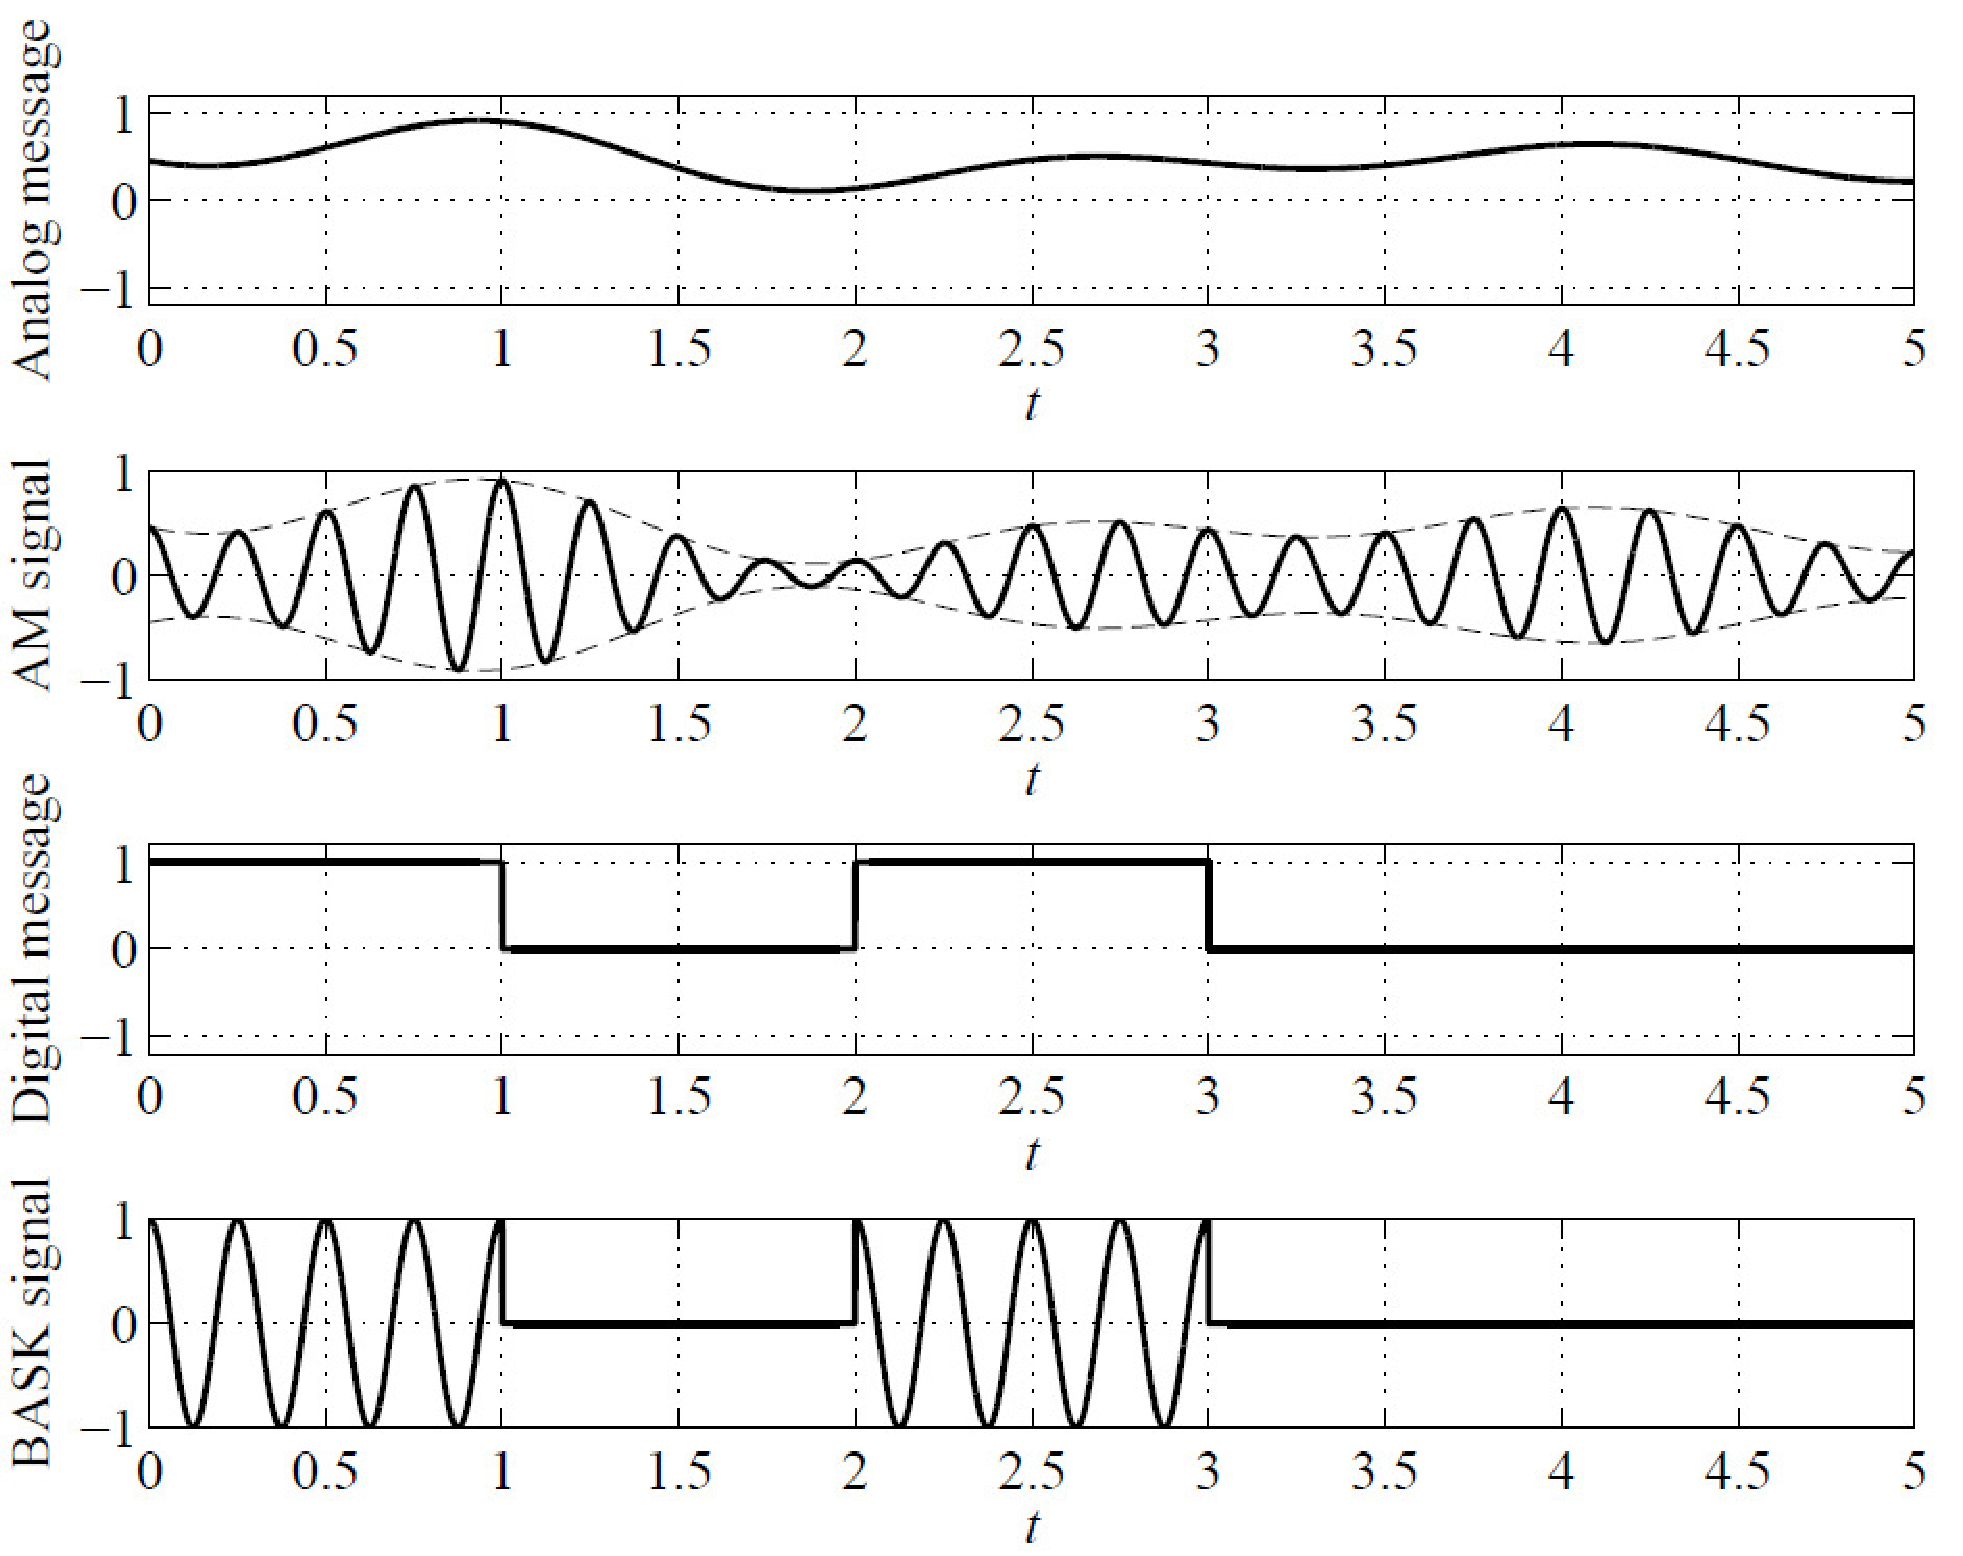
\includegraphics[width=0.77\columnwidth]{figs/fig01}
	  \end{center}
	\end{figure}

\end{frame}

\begin{frame}
    \frametitle{O que é comunicação digital?}
    
    \begin{figure}[t]
	  \begin{center}
	    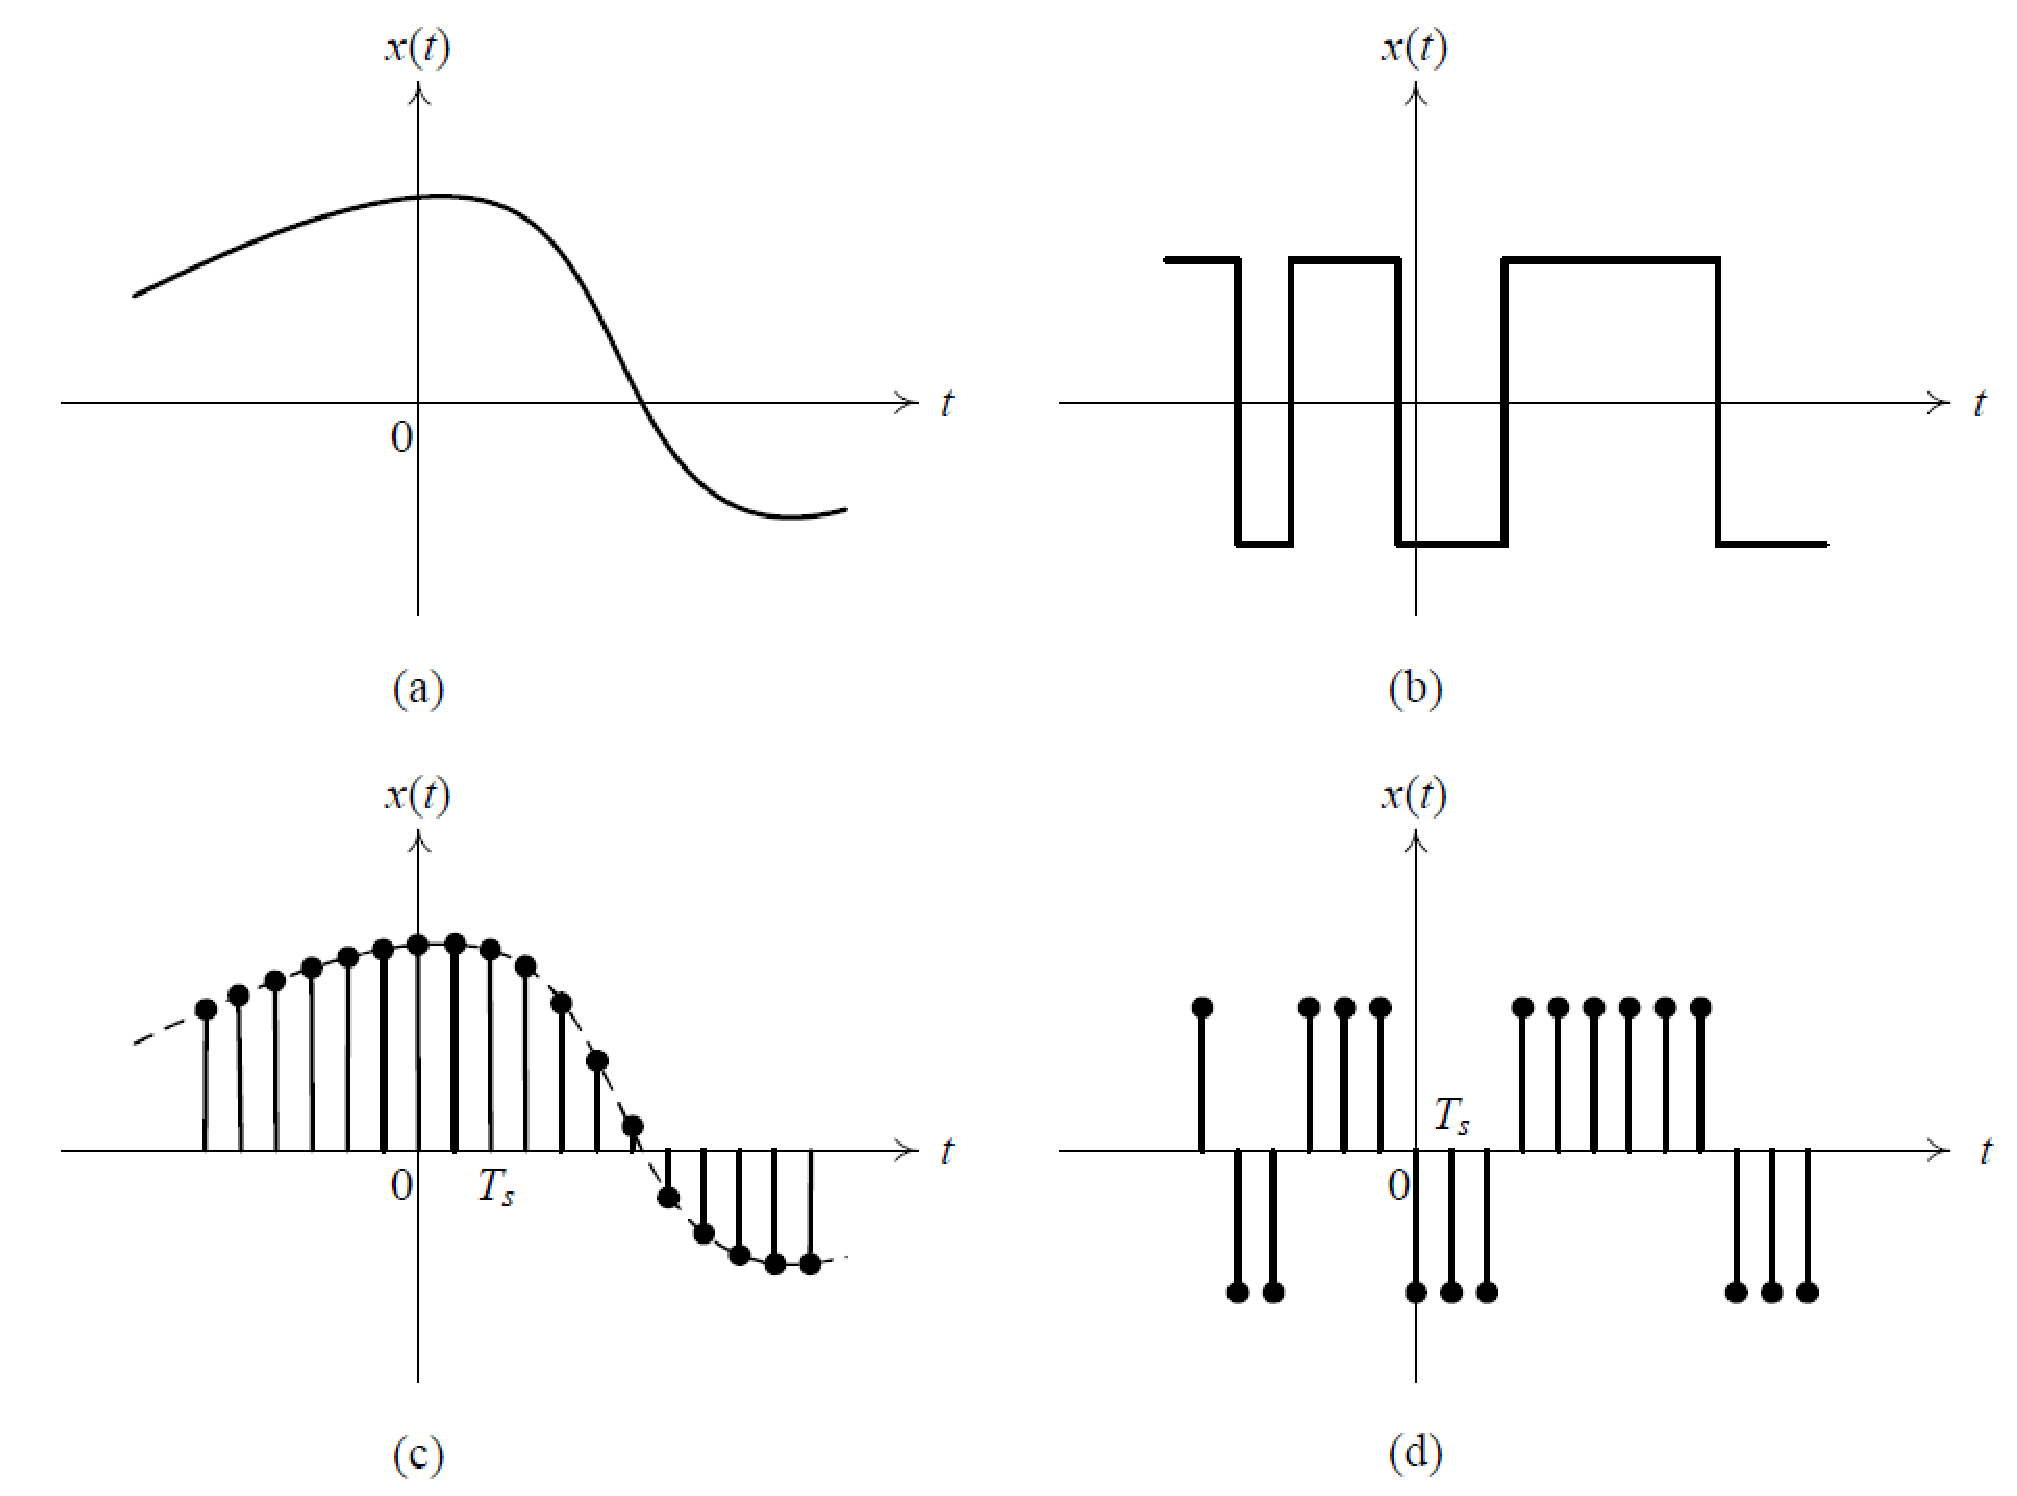
\includegraphics[width=0.77\columnwidth]{figs/fig02}
	  \end{center}
	\end{figure}
\end{frame}

\begin{frame}
    \frametitle{Por quê comunicação digital?}
    
    \begin{figure}[t]
	  \begin{center}
	    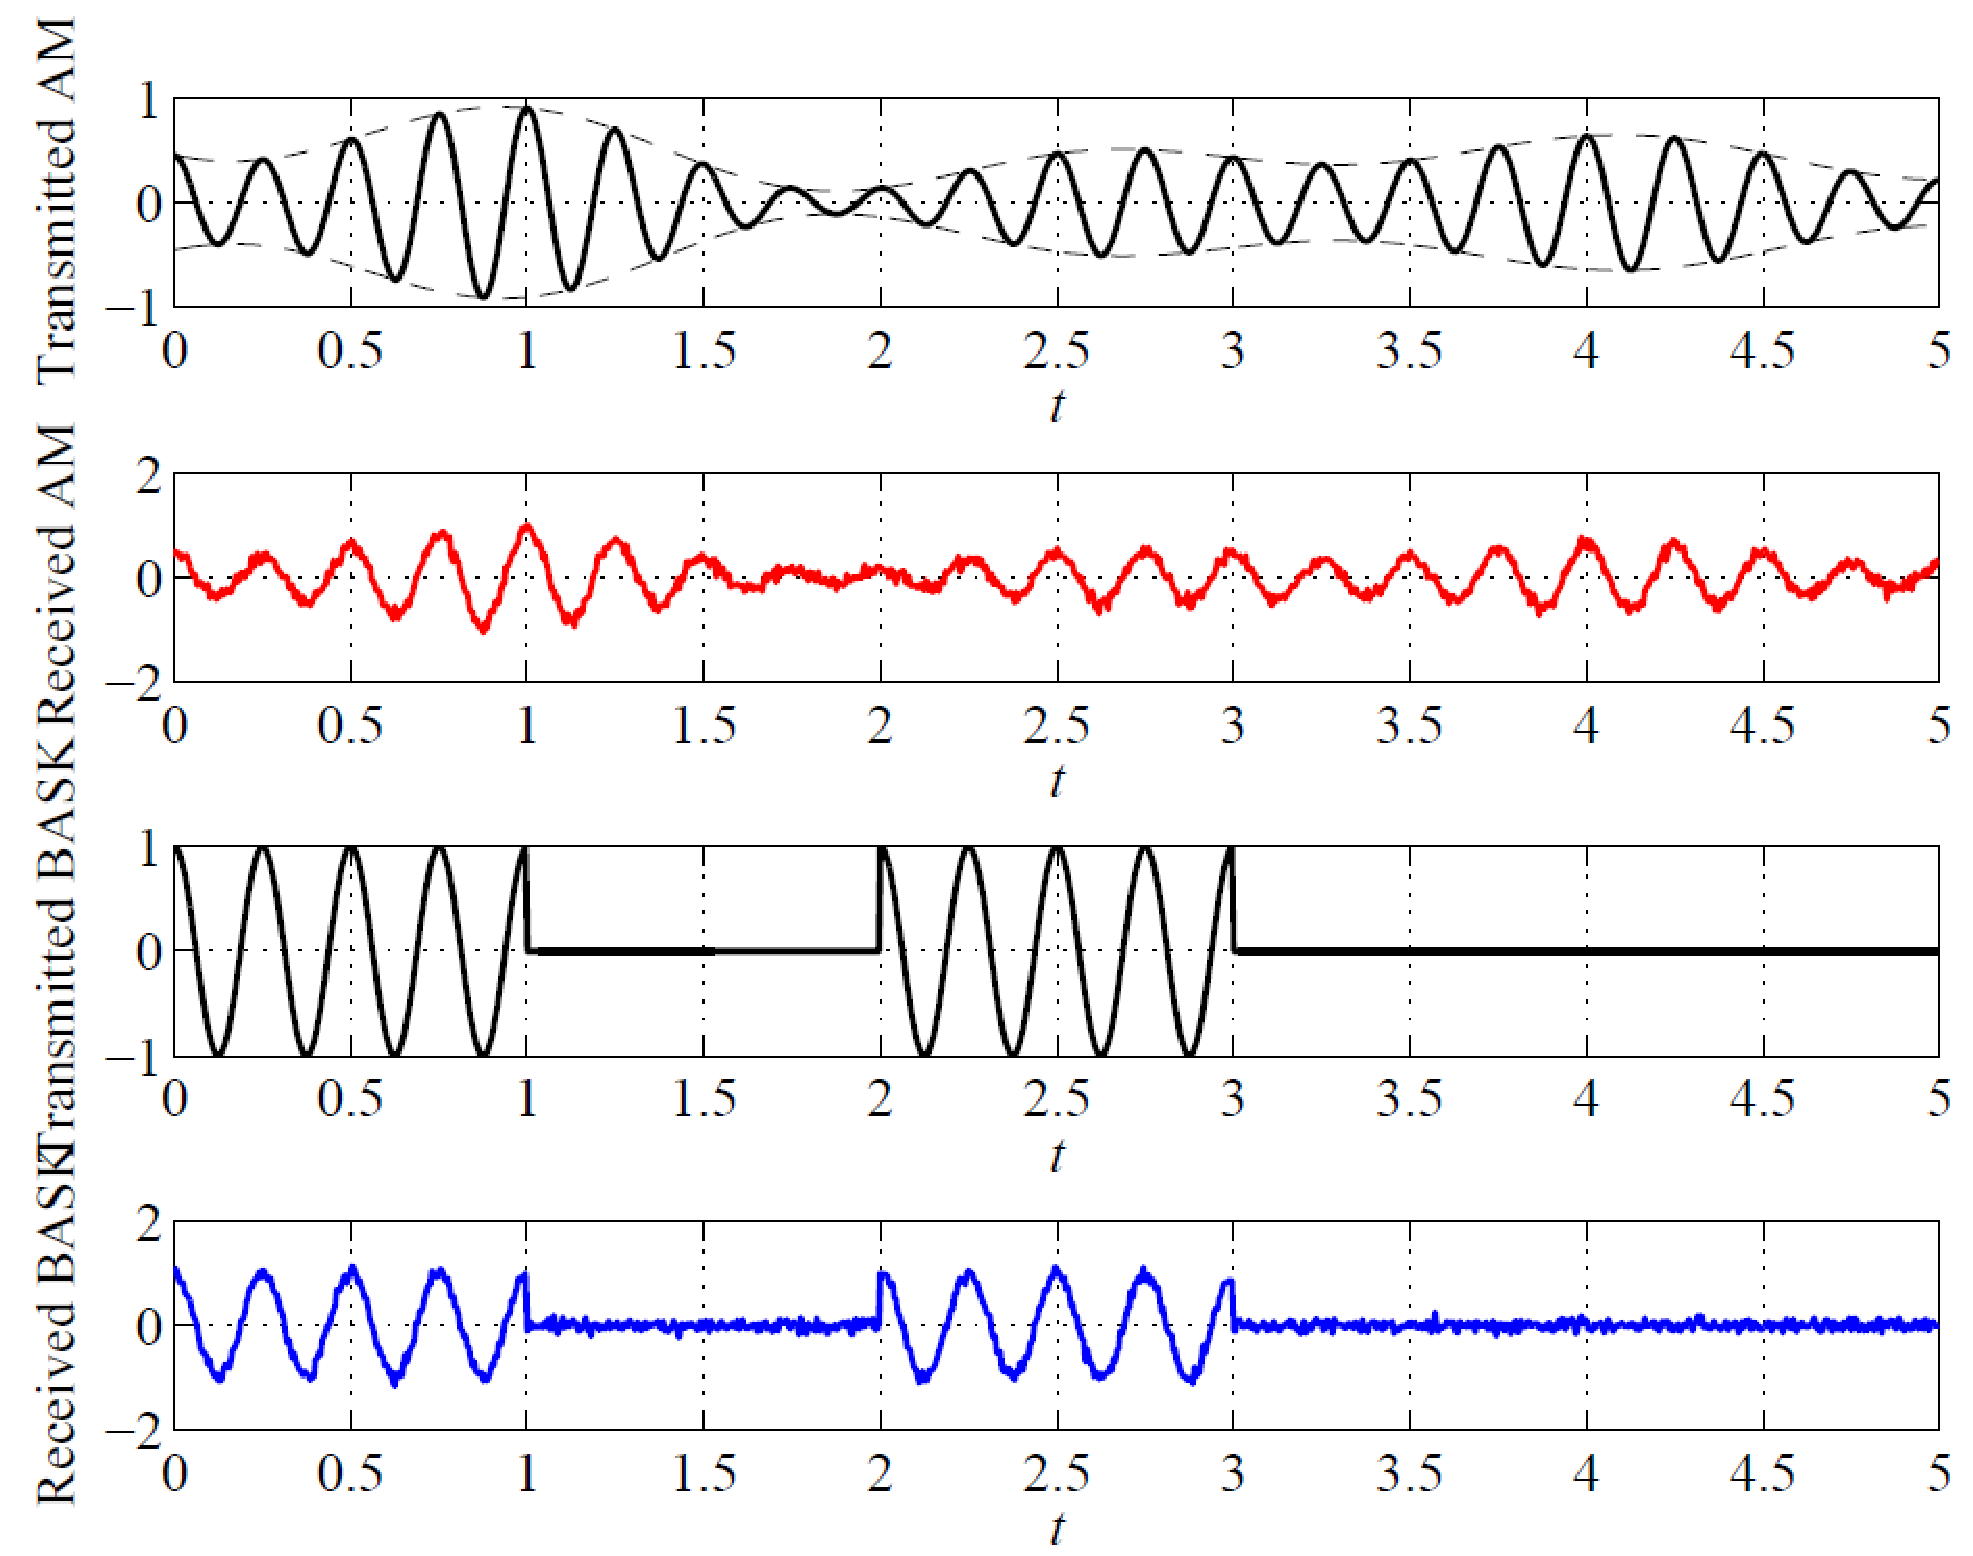
\includegraphics[width=0.77\columnwidth]{figs/fig03}
	  \end{center}
	\end{figure}
\end{frame}

\begin{frame}
    \frametitle{Por quê comunicação digital?}
    
    \begin{figure}[t]
	  \begin{center}
	    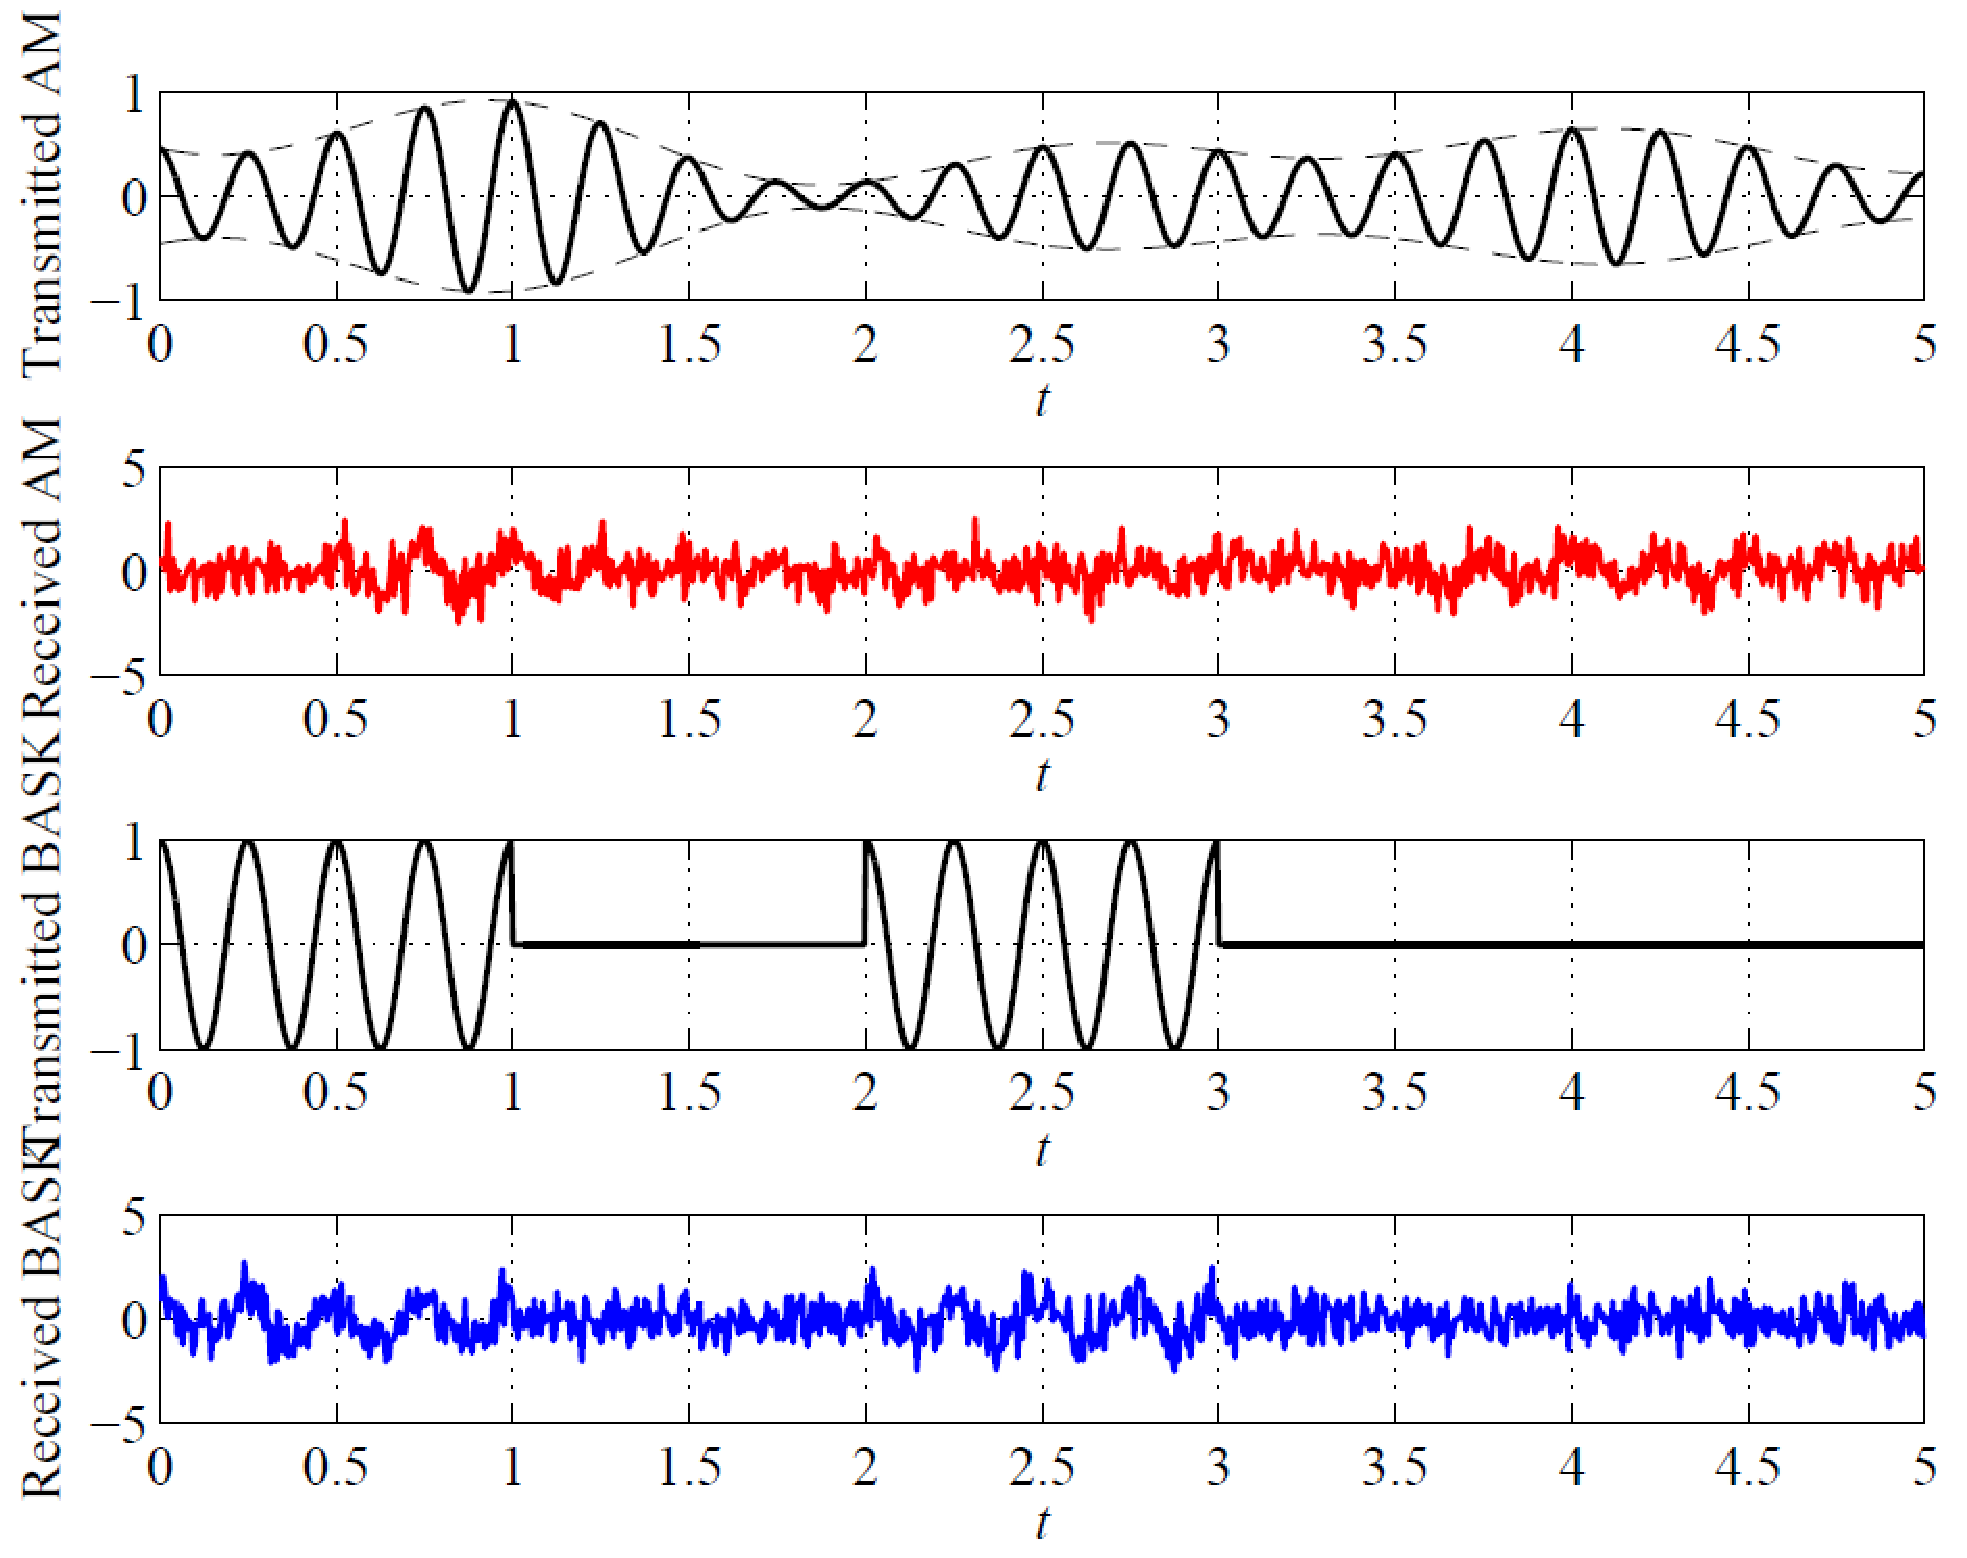
\includegraphics[width=0.77\columnwidth]{figs/fig04}
	  \end{center}
	\end{figure}
\end{frame}

\begin{frame}
    \frametitle{Repetidor regenerativo}
    
    \begin{figure}[t]
	  \begin{center}
	    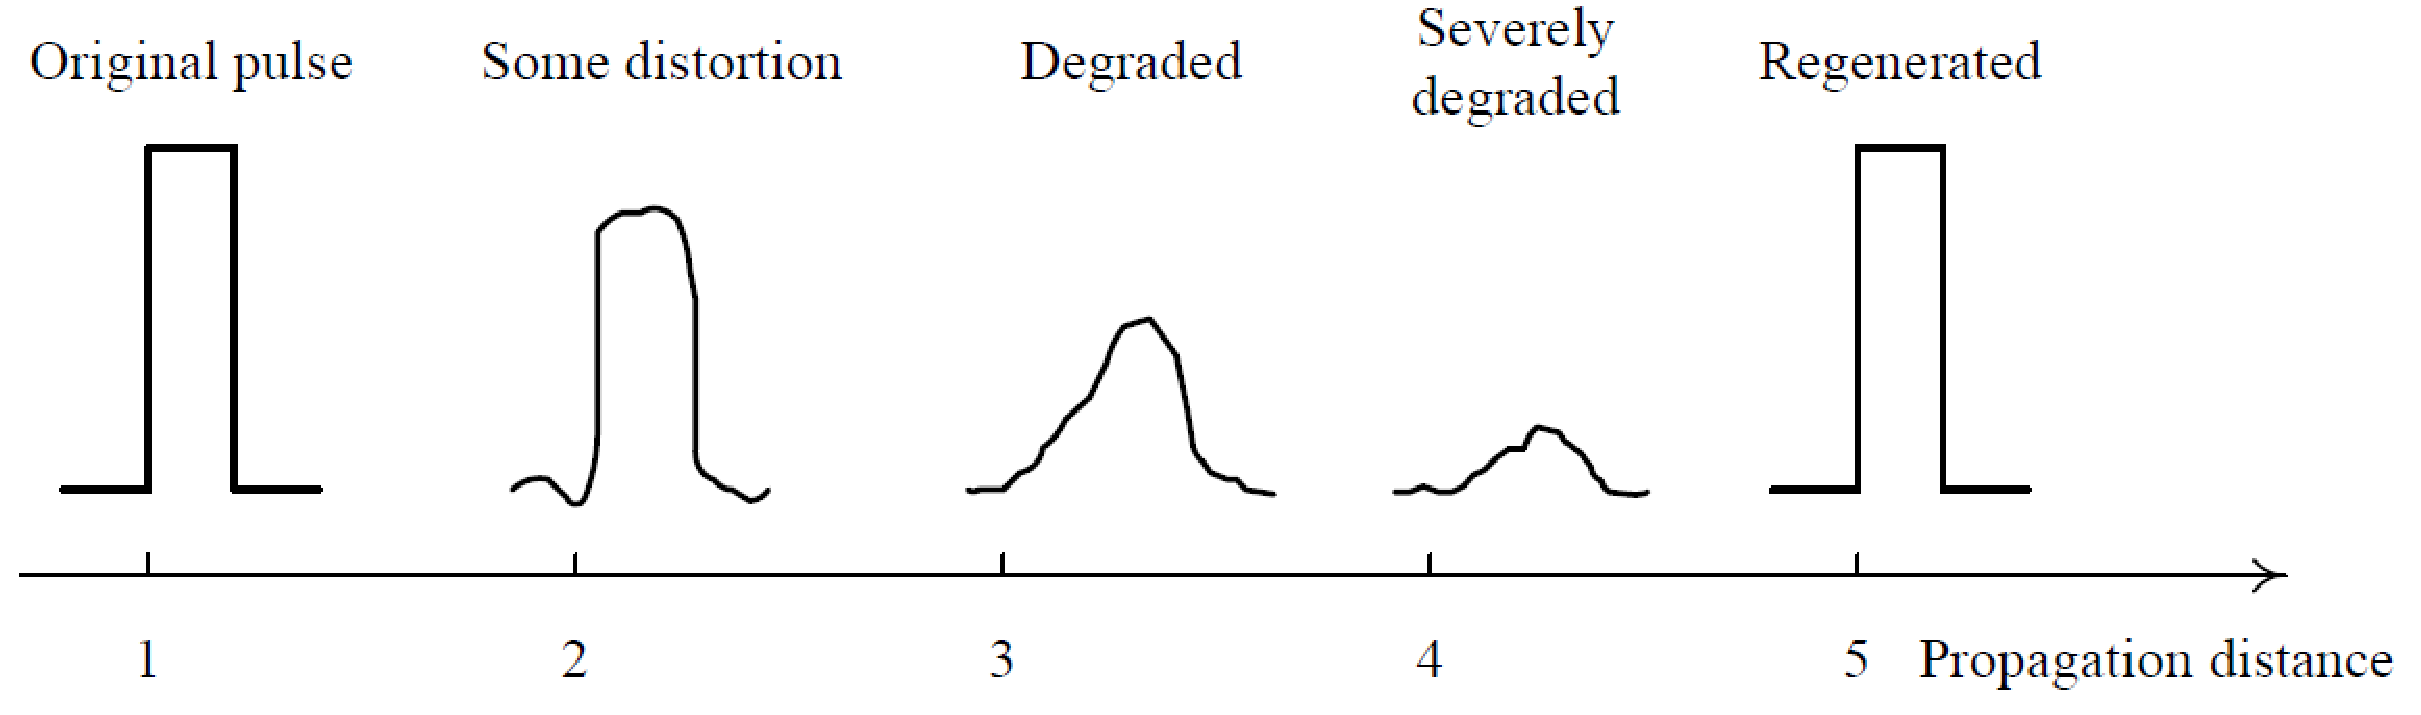
\includegraphics[width=0.77\columnwidth]{figs/fig05}
	  \end{center}
	\end{figure}
    \begin{itemize}
     \item Comunicações digitais: os sinais transmitidos pertencem a um conjunto finito de formas de onda $\Rightarrow$ O sinal distorcido pode ser recuperado para a sua forma ideal, portanto removendo totalmente o ruído.
      \item Comunicações analógicas: os sinais transmitidos são formas de onda analógicas, as quais podem assumir uma variedade infinita de formas $\Rightarrow$ Uma vez distorcido o sinal, a distorção dificilmente pode ser removida.
    \end{itemize}
\end{frame}

\begin{frame}
    \frametitle{Diagrama de blocos de um sistema de comunicação}
    
    \begin{figure}[t]
	  \begin{center}
	    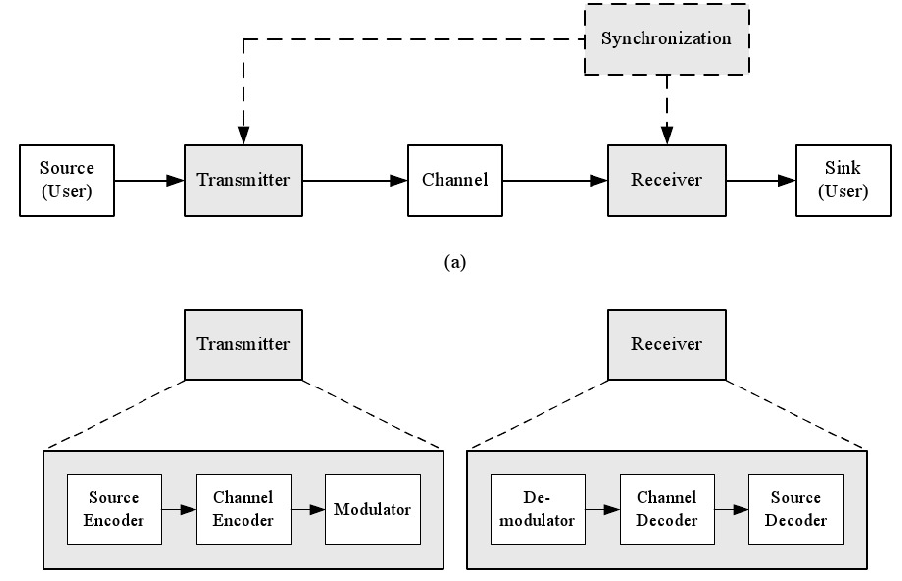
\includegraphics[width=0.77\columnwidth]{figs/fig06}
	  \end{center}
	\end{figure}
\end{frame}

\begin{frame}
    \frametitle{Digital vs. Analógico}
    
    \begin{itemize}
     \item Vantagens:
	\begin{itemize}
	 \item Sinais digitais são mais fáceis de serem regenerados.
	  \item Circuitos digitais estão menos sujeitos a distorção e interferência.
	  \item Circuitos digitais são mais confiáveis e podem ser produzidos a um custo menor do que circuitos analógicos.
	  \item A implementação de hardware digital é mais flexível que a de hardware analógico.
	  \item Sinais digitais podem se beneficiar de técnicas de processamento digital de sinais.
	\end{itemize}
     \item Desvantagens:
	\begin{itemize}
	 \item Processamento de sinais mais intenso. 
	  \item A sincronização é uma questão crucial.
	  \item Requer maior banda de transmissão.
	  \item Degradação não-suave.
	\end{itemize}
    \end{itemize}
\end{frame}

\section{Probabilidade e variáveis aleatórias}

\begin{frame}
    \frametitle{Espaço amostral e probabilidade}
    
    \begin{itemize}
     \item \textit{Experimento aleatório}: seu resultado, por algum motivo, não pode ser previsto com absoluta certeza.
      \item Exemplos: arremesso de um dado ou moeda, ou retirada de uma carta de uma pilha.
      \item \textit{Espaço amostral}: o conjunto de todos os possíveis resultados, denotado por $\Omega$. Os resultados individuais são denotados por $\omega$, onde $\omega \in \Omega$.
      \item Um espaço amostral pode ser \textit{discreto} ou \textit{contínuo}.
      \item \textit{Eventos} são subconjuntos do espaço amostral para os quais medidas de suas ocorrências, chamadas de probabilidades, podem ser definidas ou determinadas.
    \end{itemize}
\end{frame}

\begin{frame}
    \frametitle{Os três axiomas da probabilidade}
    
    \begin{itemize}
     \item Para um espaço amostral discreto $\Omega$, define-se a medida de probabilidade $P$ em $\Omega$ como uma função que assinala valores não-negativos a todos os eventos, denotados por $E$, em $\Omega$, tal que as seguintes condições são satisfeitas:
    \begin{itemize}
     \item Axioma 1: $0 \leq P(E) \leq 1$ para todo $E \in \Omega$.
     \item Axioma 2: $P(\Omega) = 1$
     \item Axioma 3: Para eventos mutuamente exclusivos, i.e., $E_i \cap E_j = \oslash \; \forall i \neq j$, tem-se que $P(\bigcup\limits_{i=1}^{\infty} E_i) = \sum\limits_{i=1}^{\infty} P(E_i)$
    \end{itemize}

    \end{itemize}
\end{frame}

\begin{frame}
    \frametitle{Propriedades importantes}
    
    \begin{enumerate}
      \item $P(E^C) = 1 - P(E)$, onde $E^C$ denota o complemento de $E$. Esta propriedade implica que $P(E^C) + P(E) = 1$, ou seja, algo tem que ocorrer.
      \item $P(\oslash) = 0$, novamente, alguma coisa tem que ocorrer.
      \item $P(E_1 \cup E_2) = P(E_1) + P(E_2) - P(E_1 \cap E_2)$. Note que se dois eventos $E_1$ e $E_2$ são mutuamente exclusivos então $P(E_1 \cup E_2) = P(E_1) + P(E_2)$.
      \item Se $E_1 \subseteq E_2$ então $P(E_1) \leq P(E_2)$. 
    \end{enumerate}
\end{frame}


\begin{frame}
    \frametitle{Probabilidade condicional}
    
    \begin{itemize}
      \item Observamos o evento $E_1$, mas na verdade estamos interessados no evento $E_2$: o conhecimento de que $E_1$ ocorreu altera a probabilidade de que $E_2$ ocorra.
      \item Se antes tinha-se $P(E_2)$, agora tem-se $P(E_2 | E_1)$, ou seja, a probabilidade de que $E_2$ ocorra dado que $E_1$ ocorreu.
      \item A probabilidade condicional é dada por
      \begin{equation}
	  P(E_2 | E_1) = \begin{cases}
			    \frac{P(E_2 \cap E_1)}{P(E_1)} \, , \quad \textrm{se} & P(E_1) \neq 0 \\
			     0 & c.c.
	                 \end{cases}
      \end{equation}

      \item Se $P(E_2| E_1) = P(E_2)$, ou $P(E_2 \cap E_1) = P(E_1) P(E_2)$, então $E_1$ e $E_2$ são ditos \textit{estatísticamente independentes}. 
      \item Regra de Bayes:
	\begin{equation}
	    P(E_2 | E_1) = \frac{P(E_1 | E_2) P(E_2)}{P(E_1)}
	\end{equation}
    \end{itemize}
\end{frame}


\begin{frame}
    \frametitle{Teorema da probabilidade total}
    
    \begin{itemize}
      \item Os eventos $\{E\}_{i=1}^n$ particionam o espaço amostral $\Omega$ se:
      \begin{itemize}
       \item $\bigcup\limits_{i=1}^n E_i = \Omega$
	\item $E_i \cap E_j = \oslash$ para todo $1 \leq i, \; j \leq n$ e $i \neq j$
      \end{itemize}
      \item Se um evento $A$ tem probabilidades condicionais $\{P(A|E_i)\}_{i=1}^n$, $P(A)$ pode ser obtido por
      \begin{equation}
	  P(A) = \sum\limits_{i=1}^n P(E_i) P(A | E_i)
      \end{equation}
      \item Regra de Bayes
      \begin{equation}
	  P(E_i | A) = \frac{P(A | E_i) P(E_i)}{P(A)} = \frac{P(A | E_i) P(E_i)}{\sum\limits_{j=1}^n P(A | E_j) P(E_j)}
      \end{equation}

    \end{itemize}
\end{frame}

\begin{frame}
    \frametitle{Variáveis aleatórias}
    
    \begin{figure}[t]
	  \begin{center}
	    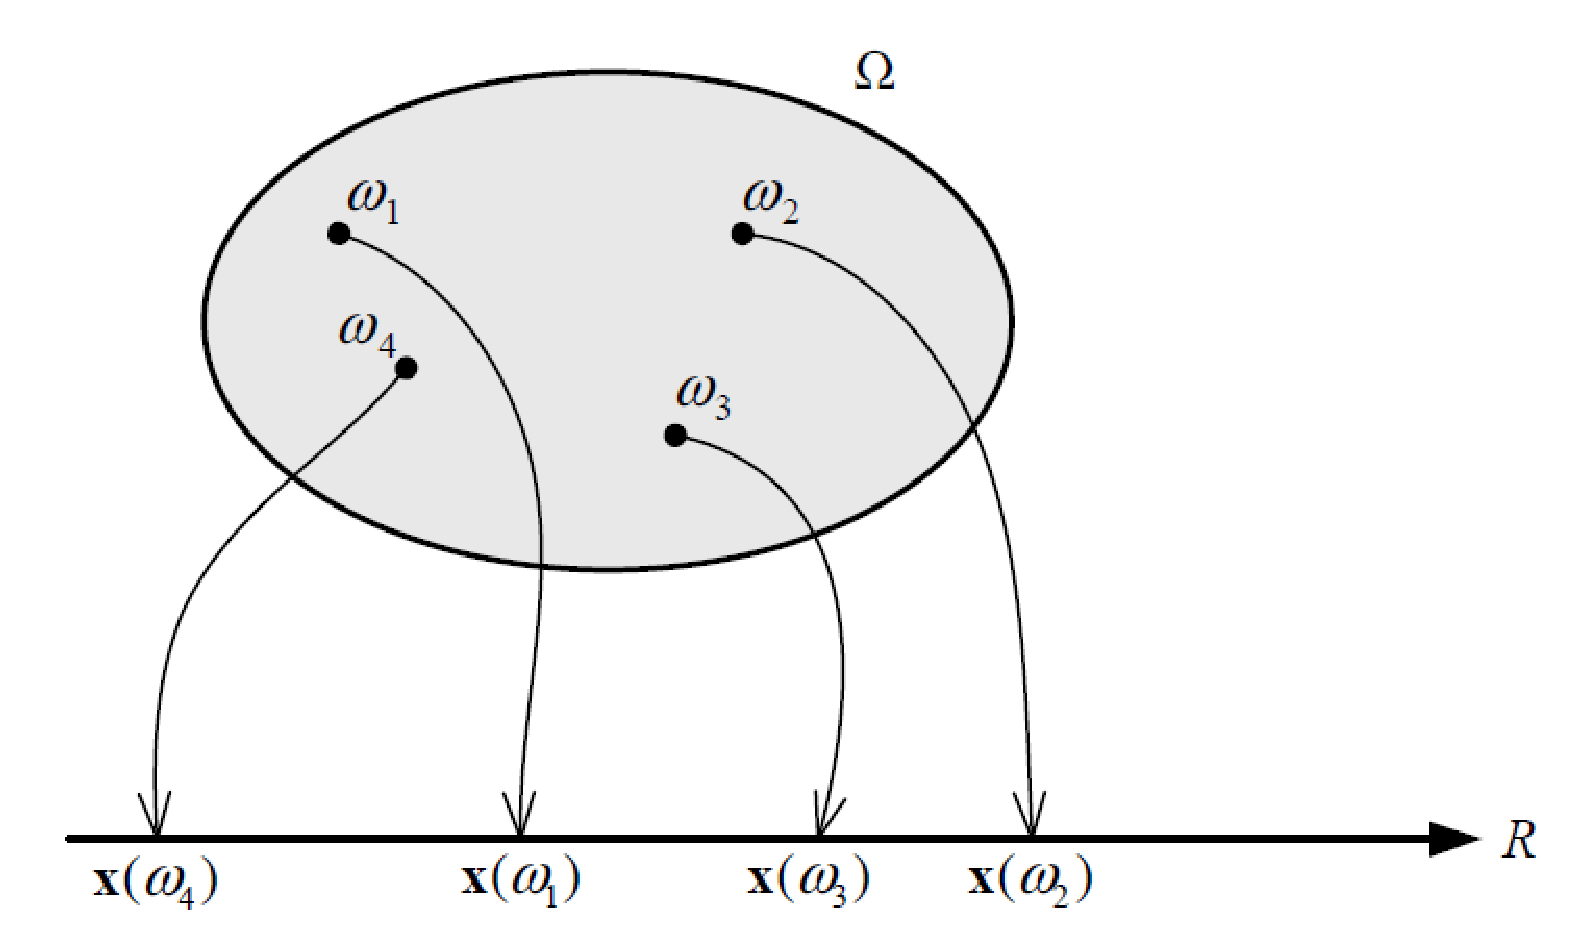
\includegraphics[width=0.6\columnwidth]{figs/fig07}
	  \end{center}
	\end{figure}

    \begin{itemize}
     \item Uma variável aleatória é um \textit{mapeamento} do espaço amostral $\Omega$ ao conjunto de números reais.
      \item Vamos expressar as variáveis aleatórias em negrito, i.e., $\mathbf{x}$, $\mathbf{y}$, etc., enquanto valores individuais ou específicos do mapeamento $\mathbf{x}$ são denotados por $\mathbf{x}(\omega)$.
    \end{itemize}

\end{frame}

\begin{frame}
    \frametitle{Função Distribuição de Probabilidade (CDF)}
    
    \begin{itemize}
      \item A CDF fornece uma descrição completa da variável aleatória. Ela é definida como:

      \begin{equation}
	  F_{\mathbf{x}}(x) = P(\omega \in \Omega \, | \, \mathbf{x}(\omega) \leq x) = P(\mathbf{x} \leq x) \, .
      \end{equation}
      
      \item A CDF possui as seguintes propriedades:
      \begin{itemize}
       \item $0 \leq F_{\mathbf{x}}(x) \leq 1$
	\item $F_{\mathbf{x}}(x)$ é não decrescente: $F_{\mathbf{x}}(x_1) \leq F_{\mathbf{x}}(x_2)$ se $x_1 \leq x_2$
	\item $F_{\mathbf{x}}(-\infty) = 0$ e $F_{\mathbf{x}}(+\infty) = 1$
	\item $P(a < \mathbf{x} \leq b) = F_{\mathbf{x}}(b) - F_{\mathbf{x}}(a)$
      \end{itemize}
    
    \end{itemize}
\end{frame}

\begin{frame}
    \frametitle{Exemplos de CDFs típicas - I}

    \begin{itemize}
     \item Uma variável aleatória pode ser \textit{discreta}, \textit{contínua} ou \textit{mista}.
    \end{itemize}

    \begin{figure}[t]
	  \begin{center}
	    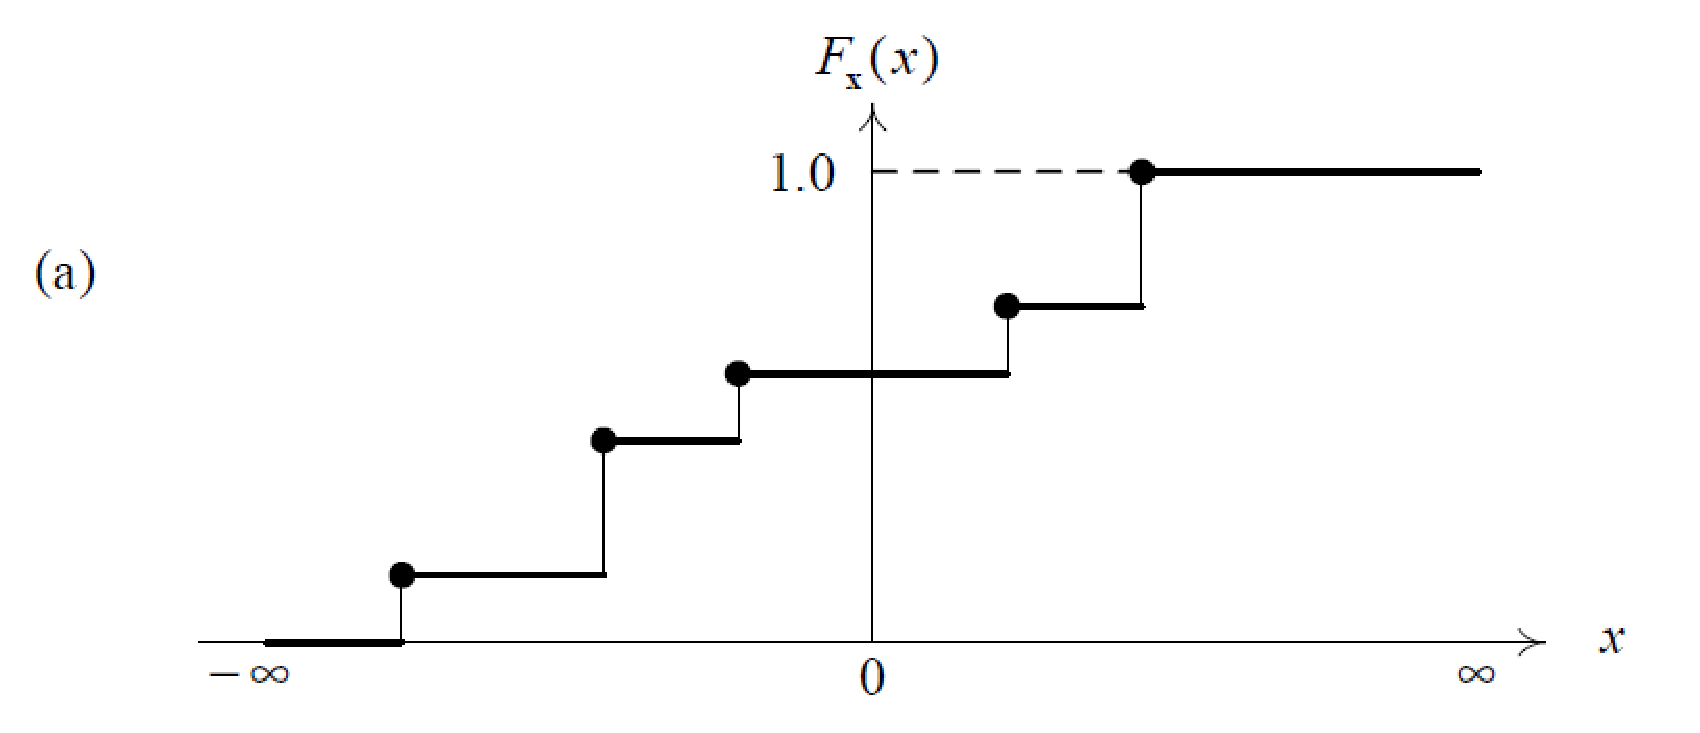
\includegraphics[width=0.77\columnwidth]{figs/fig08}
	  \end{center}
	\end{figure}
    
\end{frame}

\begin{frame}
    \frametitle{Exemplos de CDFs típicas - II}

    \begin{figure}[t]
	  \begin{center}
	    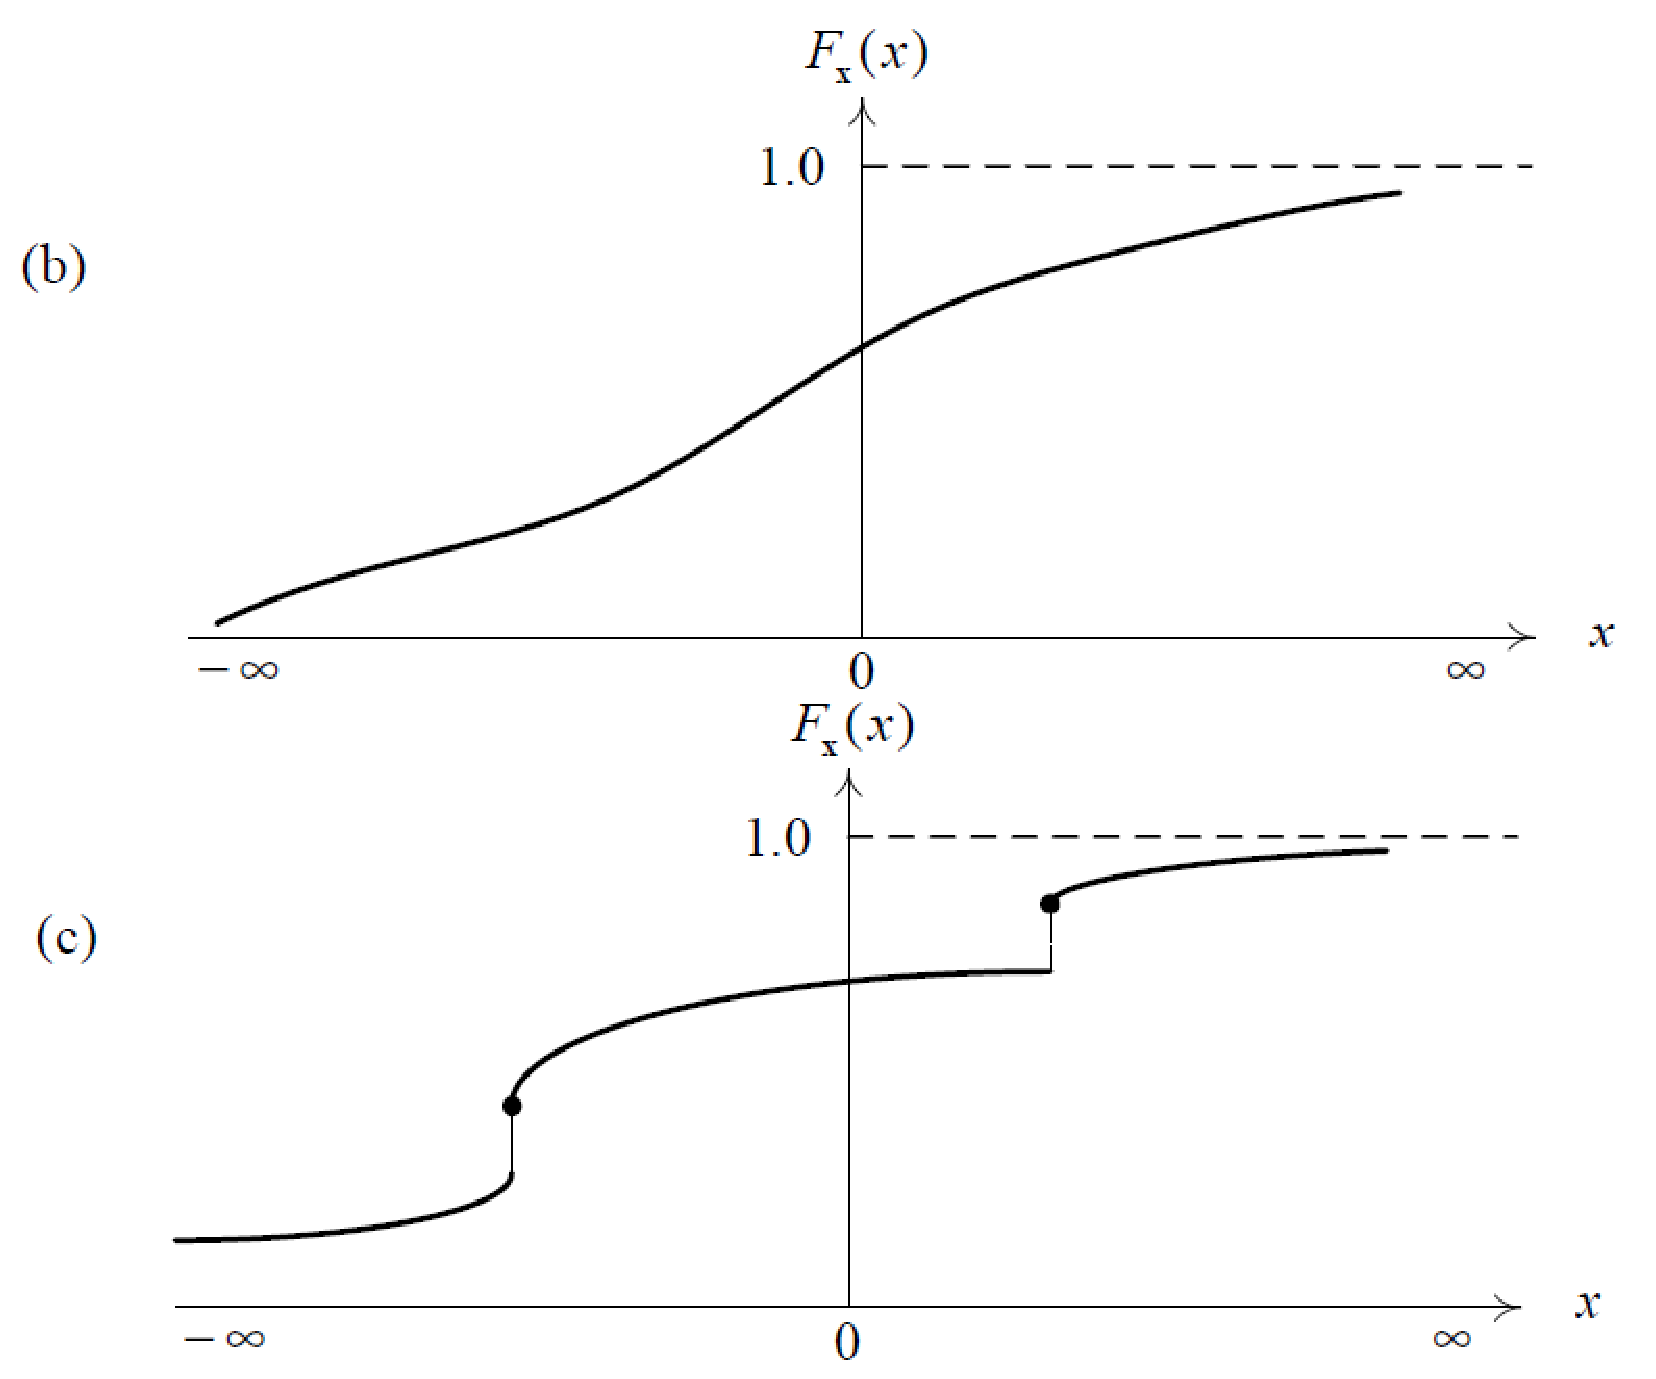
\includegraphics[width=0.7\columnwidth]{figs/fig09}
	  \end{center}
	\end{figure}
    
\end{frame}

\begin{frame}
    \frametitle{Função Densidade de Probabilidade (PDF)}
    
    \begin{itemize}
      \item A PDF é definida como a derivada da CDF:

      \begin{equation}
	  f_{\mathbf{x}}(x) = \frac{\mathrm{d} F_{\mathbf{x}}(x)}{ \mathrm{d} x} \, ; \quad F_{\vax}(x) = \int_{-\infty}^{x} f_{\vax}(u) du
      \end{equation}

      \item Segue que:
      \begin{align}
	  P(x_1 \leq \mathbf{x} \leq x_2) &= P(\mathbf{x} \leq x_2) - P(\mathbf{x} \leq x_1) \\
	  &= F_{\mathbf{x}}(x_2) - F_{\mathbf{x}}(x_1) = \int_{x_1}^{x_2}  f_{\mathbf{x}}(x)  \mathrm{d} x \, .
      \end{align}
      
      \item A PDF possui as seguintes propriedades:
      \begin{itemize}
       \item $f_{\mathbf{x}}(x) \geq 0$
	\item $\int_{-\infty}^{\infty} f_{\mathbf{x}}(x) \mathrm{d} x = 1$
	\item Em geral, $P(\mathrm{x} \in \mathcal{A}) = \int_{\mathcal{A}} f_{\mathbf{x}}(x) \mathrm{d} x$
      \end{itemize}

      \item Para variáveis aleatórias discretas é mais comum definir a função de probabilidade de massa (pmf): $p_i = P(\mathbf{x} = x_i)$.

      \item Note que, para todo $i$, temos que $p_i \geq 0$ e $\sum\limits_i p_i = 1$.
    
    \end{itemize}
\end{frame}

\begin{frame}
    \frametitle{Variável Aleatória Gaussiana}

    \begin{figure}[t]
	  \begin{center}
	    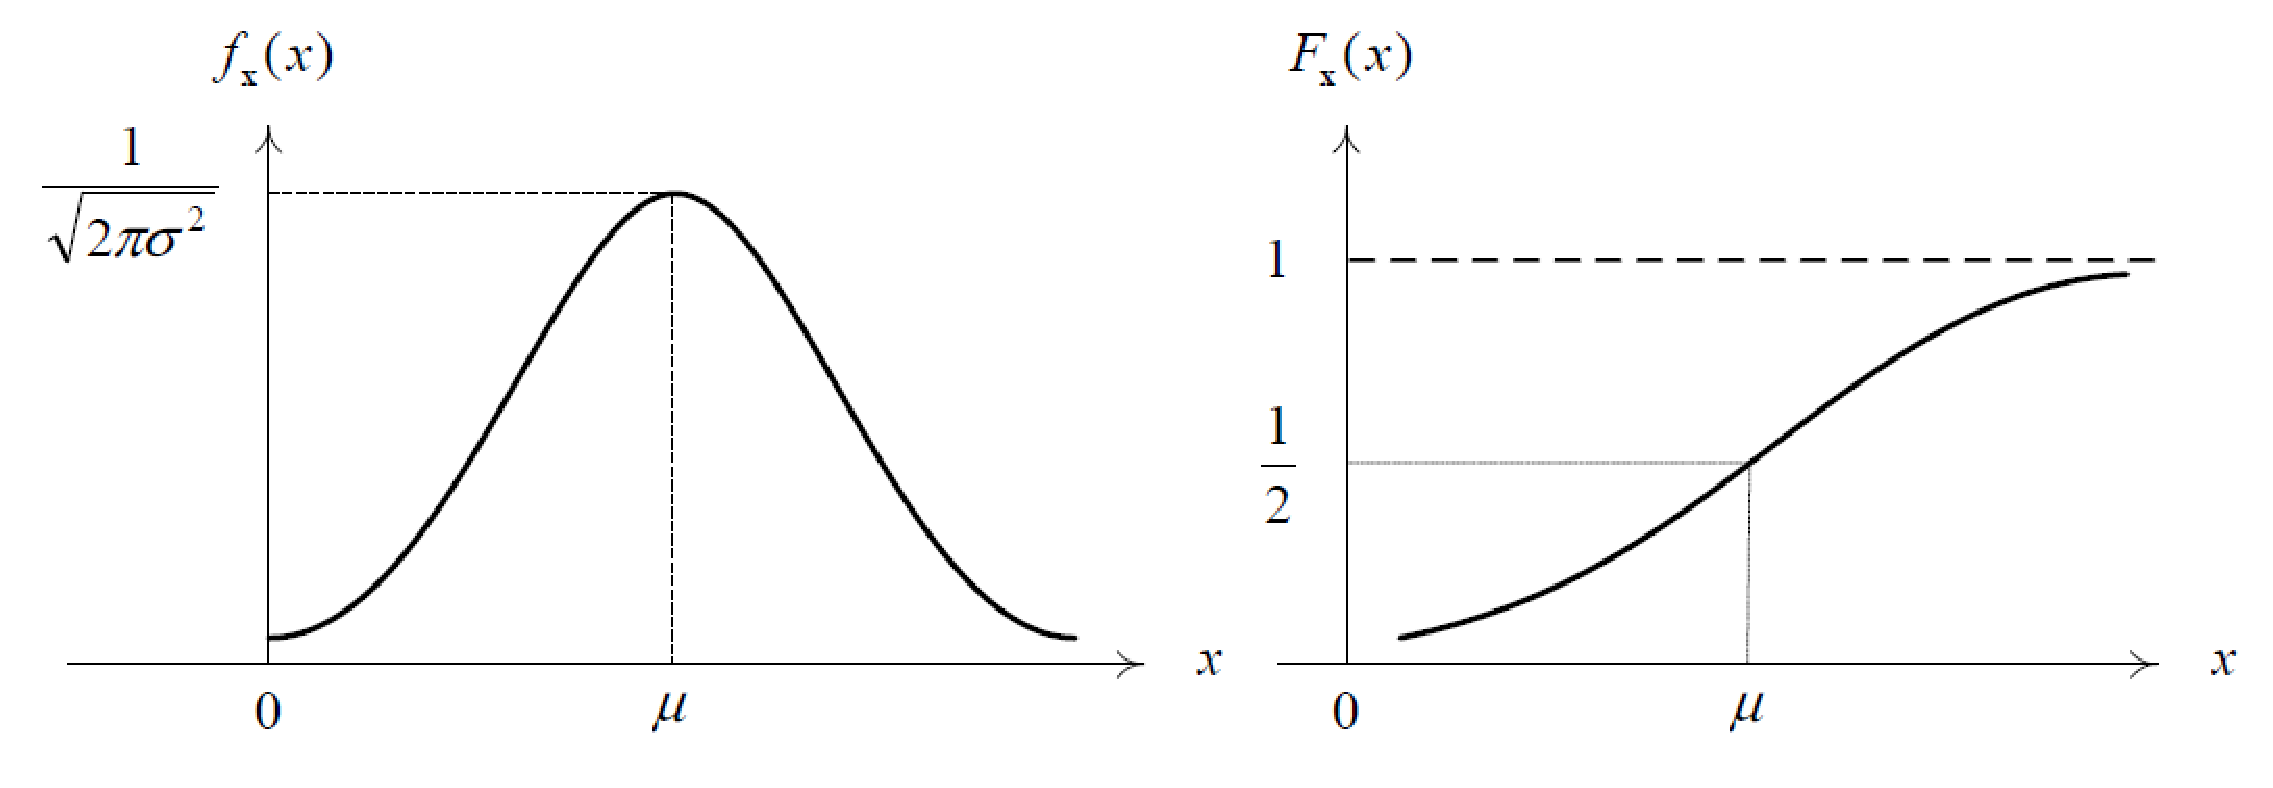
\includegraphics[width=0.77\columnwidth]{figs/fig13}
	  \end{center}
	\end{figure}

    \begin{itemize}
     \item É uma variável aleatória contínua cuja PDF é dada por:

      \begin{equation}
	  f_{\mathbf{x}}(x) = \frac{1}{\sqrt{2\pi\sigma^2}} \exp \left\{-\frac{(x-\mu)^2}{2\sigma^2}\right\} \, ,
      \end{equation}

      onde $\mu$ e $\sigma^2$ são parâmetros. É usualmente denotada por $\mathcal{N}(\mu,\sigma^2)$.
      \item É a variável aleatória mais importante e mais freqüentemente encontrada na área de comunicações.
    \end{itemize}
   
\end{frame}

\begin{frame}
    \frametitle{Variável Aleatória Gaussiana}

    \begin{itemize}
     \item Funções auxiliares:
      \begin{align}
	   \mathrm{erf}(x) &= \frac{2}{\sqrt{\pi}} \int_0^x e^{-t^2} dt \\
	   \mathrm{erfc}(x) &= \frac{2}{\sqrt{\pi}} \int_x^{\infty} e^{-t^2} dt  = 1 - \mathrm{erf}(x) \\
	   \mathrm{Q}(x) &= \frac{1}{\sqrt{2\pi}} \int_x^{\infty} e^{-t^2/2} dt  = \frac{1}{2}\mathrm{erfc}\left(\frac{x}{\sqrt{2}}\right)
      \end{align}

     \item CDF Gaussiana:

      \begin{align}
	  F_{\mathbf{x}}(x) &= \int_{-\infty}^x \frac{1}{\sqrt{2\pi\sigma^2}} \exp \left\{-\frac{(t-\mu)^2}{2\sigma^2}\right\} dt \\
	  F_{\mathbf{x}}(x) &= 1 - \frac{1}{2}\mathrm{erfc}\left( \frac{x - \mu}{\sqrt{2}\sigma} \right)
      \end{align}

    \end{itemize}

\end{frame}

\begin{frame}
    \frametitle{Variável Aleatória Gaussiana}

    \begin{figure}[t]
	  \begin{center}
	    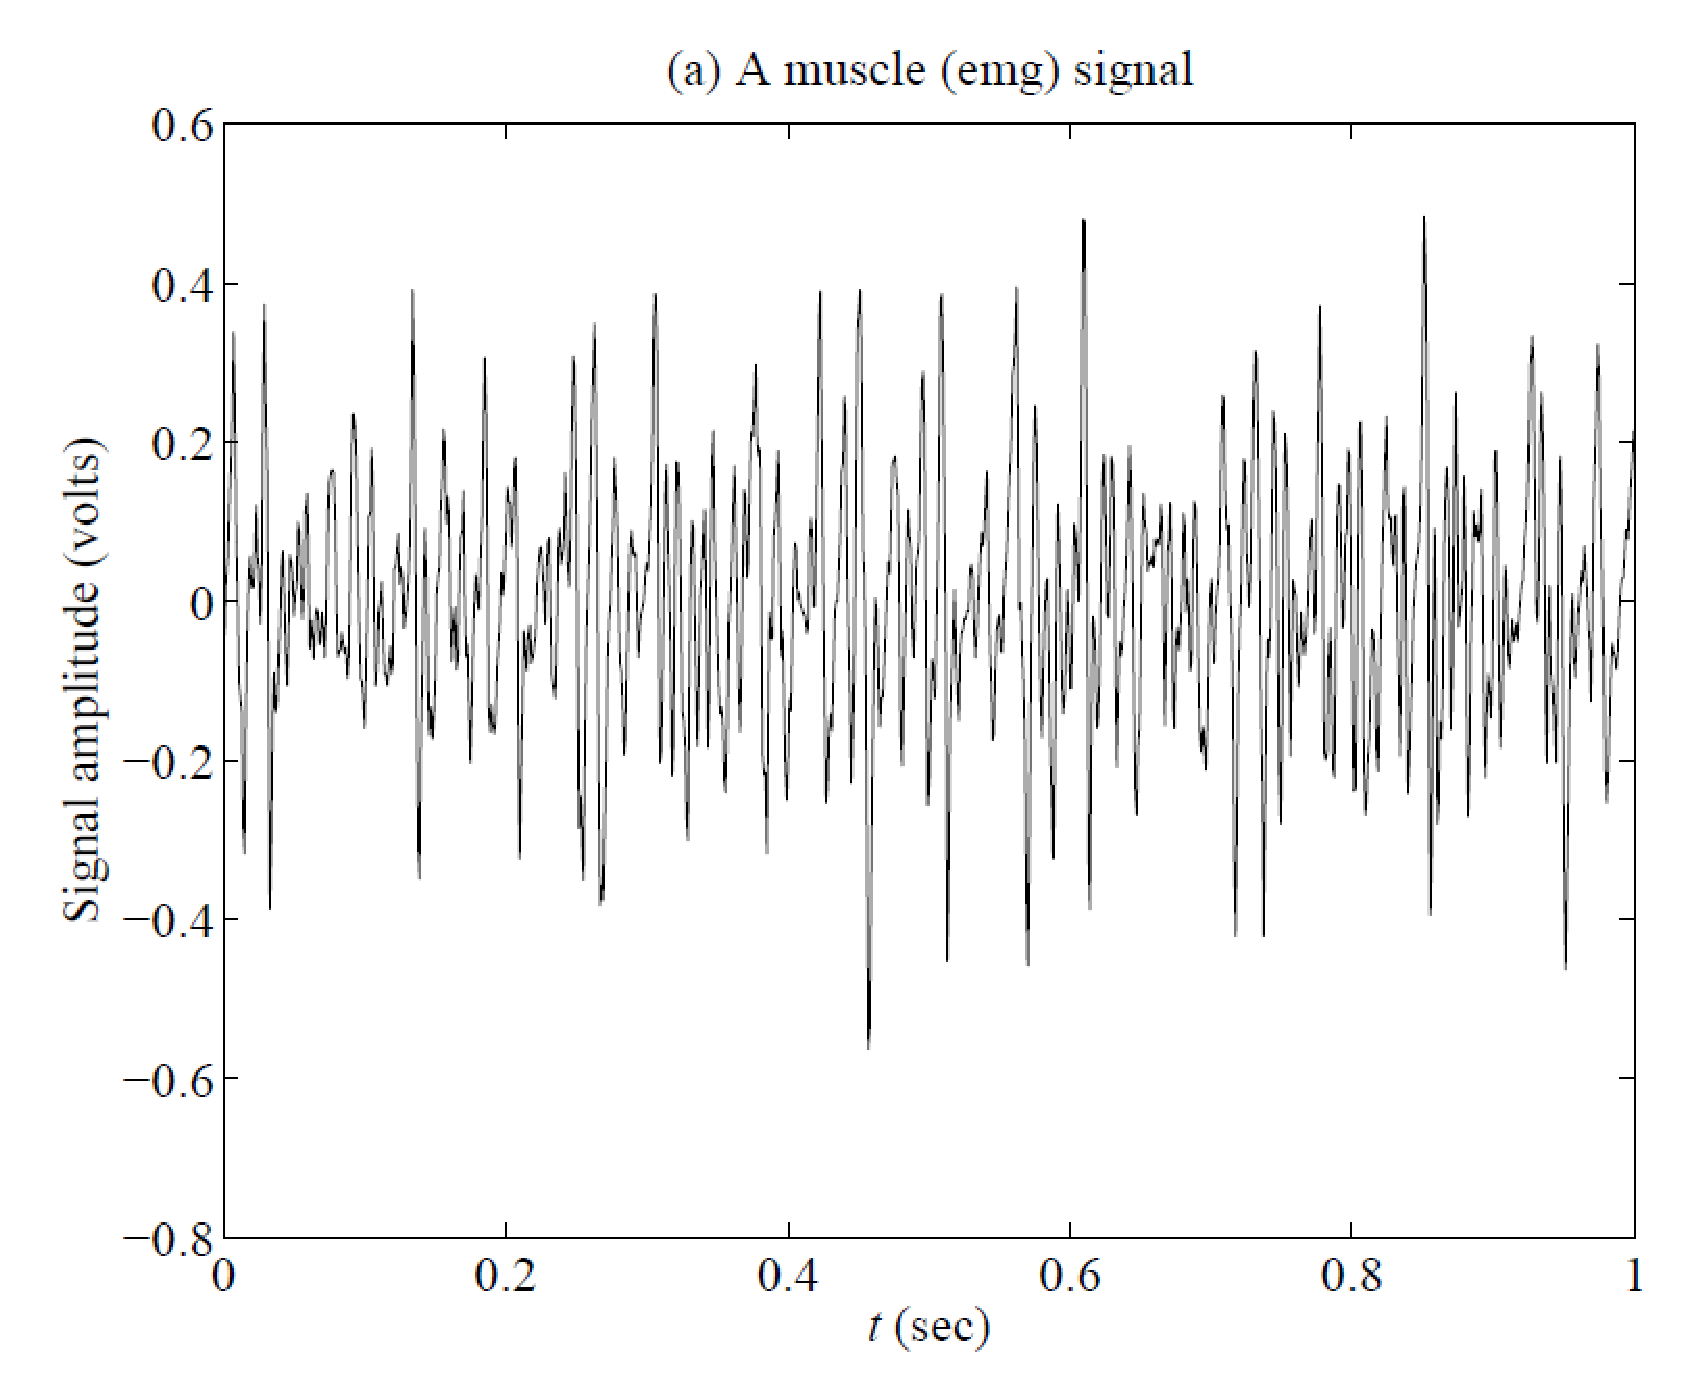
\includegraphics[width=0.77\columnwidth]{figs/fig14}
	  \end{center}
	\end{figure}
\end{frame}

\begin{frame}
    \frametitle{Variável Aleatória Gaussiana}

    \begin{figure}[t]
	  \begin{center}
	    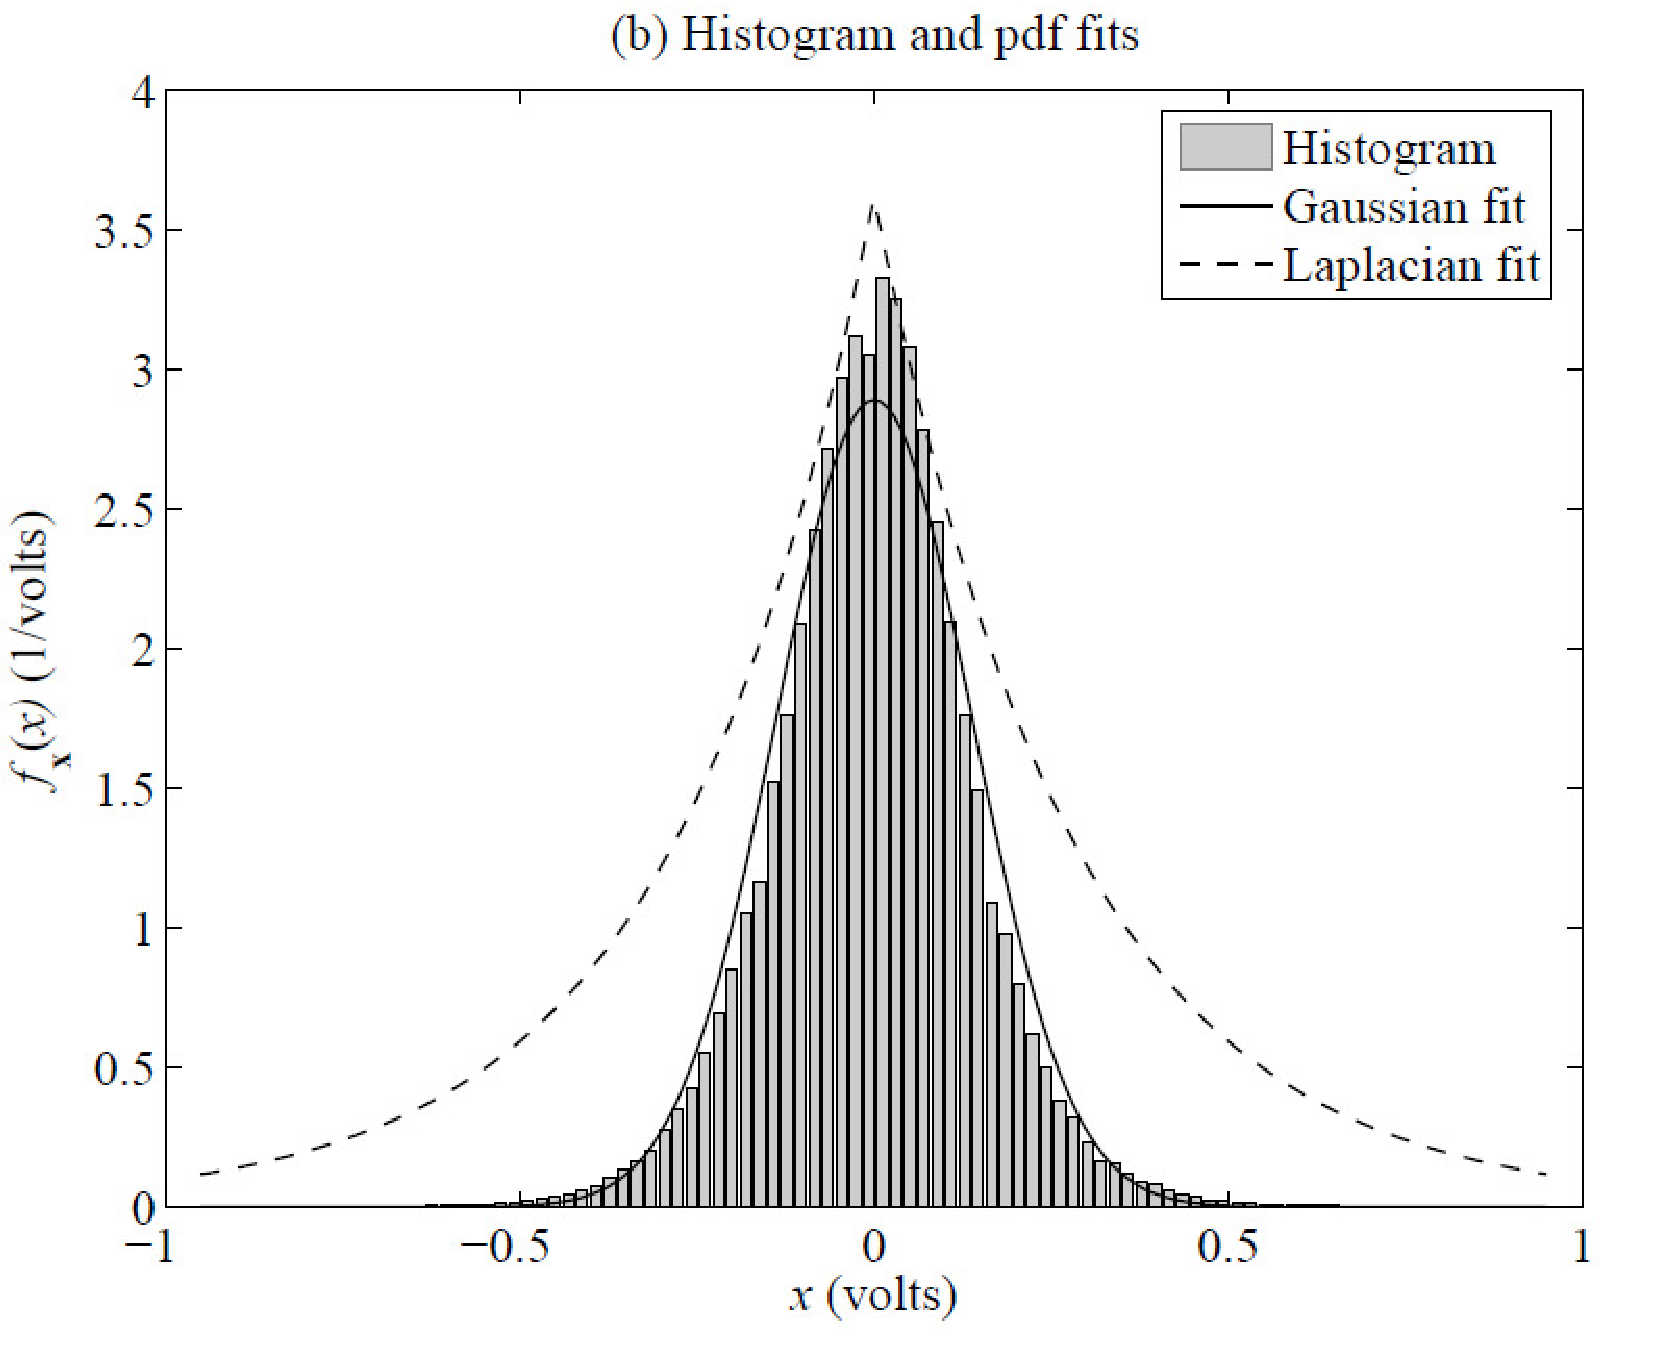
\includegraphics[width=0.77\columnwidth]{figs/fig15}
	  \end{center}
	\end{figure}
\end{frame}

\begin{frame}
    \frametitle{Funções de uma variável aleatória}

    \begin{itemize}
     \item A função $\mathbf{y} = g(\mathbf{x})$ é também uma variável aleatória.
      \item Pela definição, a CDF de $\mathbf{y}$ pode ser escrita como

      \begin{equation}
	  F_{\mathbf{y}}(y) = P(\omega \in \Omega \, | g(\mathbf{x}(\omega)) \leq y) \, ,
      \end{equation}

      \item Assuma que para todo $y$, a equação $g(x) = y$ possui um número de soluções finito e em cada ponto da solução, a derivada de $g(x)$ existe e é não-nula. A PDF de $\mathbf{y} = g(\mathbf{x})$ é dada por:

      \begin{equation}
	  f_{\mathbf{y}}(y) = \sum\limits_i \frac{f_{\mathbf{x}}(x_i)}{\left| \left. \frac{\mathrm{d}g(x)}{\mathrm{d}x} \right|_{x = x_i}  \right|} \, ,
      \end{equation}
      onde $\{x_i\}$ são as soluções de $g(x) = y$.
      \item Uma função linear de uma variável aleatória Gaussiana é também uma variável aleatória Gaussiana.

    \end{itemize}
   
\end{frame}

\begin{frame}
    \frametitle{Esperança de variáveis aleatórias - I}

    \begin{itemize}
     \item \textit{Médias estatísticas}, ou \textit{momentos}, possuem um papel importante na caracterização de uma variável aleatória.
     \item O \textit{valor esperado} (também chamado de valor médio ou primeiro momento) de uma variável aleatória $\mathbf{x}$ é definido como:

    \begin{equation}
	m_{\mathbf{x}} = E\{\mathbf{x}\} = \int_{-\infty}^{\infty} x f_{\mathbf{x}}(x) \mathrm{d}x \, ,
    \end{equation}
    onde $E$ denota o \textit{operador estatístico esperança}.
    \item Em geral, o n-ésimo momento de $\mathbf{x}$ é definido como:
    \begin{equation}
	E\{\mathbf{x}^n\} = \int_{-\infty}^{\infty} x^n f_{\mathbf{x}}(x) \mathrm{d}x \, .
    \end{equation}
    \item Para $n=2$, $E\{\mathbf{x}^2\}$ é conhecido como o valor médio quadrático da variável aleatória.
    \end{itemize}
   
\end{frame}

\begin{frame}
    \frametitle{Esperança de variáveis aleatórias - II}

    \begin{itemize}
     \item O n-ésimo \textit{momento central} da variável aleatória $\mathbf{x}$ é:

      \begin{equation}
	E\{\mathbf{y}\} = E\{(\mathbf{x} - m_{\mathbf{x}})^n\} = \int_{-\infty}^{\infty} (x-m_{\mathbf{x}})^n f_{\mathbf{x}}(x) \mathrm{d}x
      \end{equation}

      \item Quando $n=2$, o momento central é chamado de \textit{variância}, comumente denotado por $\sigma_{\mathbf{x}}^2$:

      \begin{equation}
	\sigma_{\mathbf{x}}^2 = \mathrm{var}(\mathbf{x}) = E\{(\mathbf{x} - m_{\mathbf{x}})^2\} = \int_{-\infty}^{\infty} (x-m_{\mathbf{x}})^2 f_{\mathbf{x}}(x) \mathrm{d}x
      \end{equation}
    
    \item A variância provê uma medida da ``aleatoriedade'' da variável.
    \item A média e variância de uma variável aleatória fornecem uma \textit{descrição parcial} de sua PDF.
    \item Relação entre a variância, o primeiro e o segundo momentos é dada por:
      \begin{equation}
	\sigma_{\mathbf{x}}^2 = E\{\mathbf{x}^2\} - [E\{\mathbf{x}\}]^2 = E\{\mathbf{x}^2\} - m_{\mathbf{x}}^2 \, .
      \end{equation}
    \end{itemize}
\end{frame}


\begin{frame}
    \frametitle{Variáveis aleatórias múltiplas - I}

    \begin{itemize}
     \item Normalmente encontradas quando tratando-se experimentos combinados ou tentativas repetidas de um único experimento.
      \item São basicamente funções multidimensionais definidas em um espaço amostral de um experimento combinado.
      \item Sejam $\mathbf{x}$ e $\mathbf{y}$ duas variáveis aleatórias definidas em um mesmo espaço amostral $\Omega$. A função distribuição de probabilidade conjunta é definida como:
      \begin{equation}
	  F_{\mathbf{x},\mathbf{y}} (x, y) = P(\mathbf{x} \leq x, \mathbf{y} \leq y)
      \end{equation}
      \item De forma análoga, a função densidade de probabilidade conjunta é dada por:
      \begin{equation}
	  f_{\mathbf{x},\mathbf{y}} (x, y) = \frac{\partial^2 F_{\mathbf{x},\mathbf{y}} (x, y)}{\partial x \partial y}
      \end{equation}
    
    \end{itemize}

\end{frame}

\begin{frame}
    \frametitle{Variáveis aleatórias múltiplas - II}

    \begin{itemize}
     \item Quando a PDF conjunta é integrada sobre uma das variáveis, uma obtém a PDF da outra variável, chamada de PDF marginal:
      \begin{align}
	  & \int_{-\infty}^{\infty} f_{\mathbf{x},\mathbf{y}} (x, y) \textrm{d}x = f_{\mathbf{y}}(y) \\
	  & \int_{-\infty}^{\infty} f_{\mathbf{x},\mathbf{y}} (x, y) \textrm{d}y = f_{\mathbf{x}}(x)
      \end{align}
      \item Note que:
      \begin{align}
	  & \int_{-\infty}^{\infty}\int_{-\infty}^{\infty} f_{\mathbf{x},\mathbf{y}} (x, y) \textrm{d}x\textrm{d}y = F(\infty, \infty) = 1 \\
	  & F_{\mathbf{x},\mathbf{y}}(-\infty,-\infty) = F_{\mathbf{x},\mathbf{y}}(-\infty,y) = F_{\mathbf{x},\mathbf{y}}(x,-\infty) = 0
      \end{align}
    
    \end{itemize}

\end{frame}

\begin{frame}
    \frametitle{Variáveis aleatórias múltiplas - III}

    \begin{itemize}
     \item A PDF condicional da variável aleatória $\mathbf{y}$, dado que o valor da variável aleatória $\mathbf{x}$ é igual a $x$, é definida como:
      \begin{equation}
      f_{\mathbf{y}}(y|x) =  \begin{cases}
				    \frac{f_{\mathbf{x},\mathbf{y}}(x,y)}{f_{\mathbf{x}}(x)} \, , & f_{\mathbf{x}}(x) \neq 0 \\
				    0 \, , & \mathrm{c.c.}
                               \end{cases}
      \end{equation}
      \item Duas variáveis aleatórias $\vax$ e $\vay$ são estatísticamente independentes se e somente se:
      \begin{align}
	  & f_{\vay}(y|x) = f_{\vay}(y) \qquad \textrm{ou de forma equivalente} \\
	  & f_{\vax,\vay}(x,y) = f_{\vax}(x)f_{\vay}(y)
      \end{align}
      \item O \textit{momento conjunto} é definido como:
      \begin{equation}
	  E\{\vax^j\vay^k\} = \int_{-\infty}^{\infty}\int_{-\infty}^{\infty} x^j y^k f_{\vax,\vay}(x,y)\mathrm{d}x\mathrm{d}y \, .
      \end{equation}
      
    \end{itemize}

\end{frame}

\begin{frame}
    \frametitle{Variáveis aleatórias múltiplas - IV}

    \begin{itemize}
     \item O \textit{momento central conjunto} é:
      \begin{equation}
	  E\{(\vax-m_{\vax})^j(\vay-m_{\vay})^k\} = \int_{-\infty}^{\infty}\int_{-\infty}^{\infty} (x-m_{\vax})^j (y-m_{\vay})^k f_{\vax,\vay}(x,y)\mathrm{d}x\mathrm{d}y \, ,
      \end{equation}
      onde $m_{\vax} = E\{\vax\}$ e $m_{\vay} = E\{\vay\}$.
      \item Os momentos mais importantes são:
      \begin{itemize}
       \item Correlação:
	\begin{equation}
	    E\{\vax\vay\} = \int_{-\infty}^{\infty}\int_{-\infty}^{\infty} x y f_{\vax,\vay}(x,y)\mathrm{d}x\mathrm{d}y
	\end{equation}
	\item Covariância:
	\begin{equation}
	    \mathrm{cov}\{\vax,\vay\} = E\{(\vax-m_{\vax})(\vay-m_{\vay})\} = E\{\vax\vay\} - m_{\vax}m_{\vay}
	\end{equation}

      \end{itemize}

    \end{itemize}
    
\end{frame}

\begin{frame}
    \frametitle{Variáveis aleatórias múltiplas - V}

    \begin{itemize}
     \item Sejam $\sigma_{\vax}^2$ e $\sigma_{\vay}^2$ as variâncias de $\vax$ e $\vay$, respectivamente. A covariância normalizada com relação a $\sigma_{\vax}\sigma_{\vay}$ é chamada de \textit{coeficiente de correlação}:
      \begin{equation}
	  \rho_{\vax,\vay} = \frac{\mathrm{cov}\{\vax,\vay\}}{\sigma_{\vax}\sigma_{\vay}} \, .
      \end{equation}
    \item $\rho_{\vax,\vay}$ indica o grau de \textit{dependência linear} entre duas variáveis aleatórias. 
    \item Pode-se mostrar que $|\rho_{\vax,\vay}| \leq 1$.
    \item Se $\rho_{\vax,\vay} = 0$, $\vax$ e $\vay$ são ditas \textit{descorrelacionadas}.
    \item Pode-se verificar que se $\vax$ e $\vay$ são independentes, então $\rho_{\vax,\vay} = 0$: \textit{independência implica em ausência de correlação}.
    \item No entanto, ausência de correlação não necessariamente implica em independência estatística.
    \end{itemize}
    
\end{frame}

\begin{frame}
    \frametitle{Processos aleatórios - I}

    \begin{figure}[t]
	  \begin{center}
	    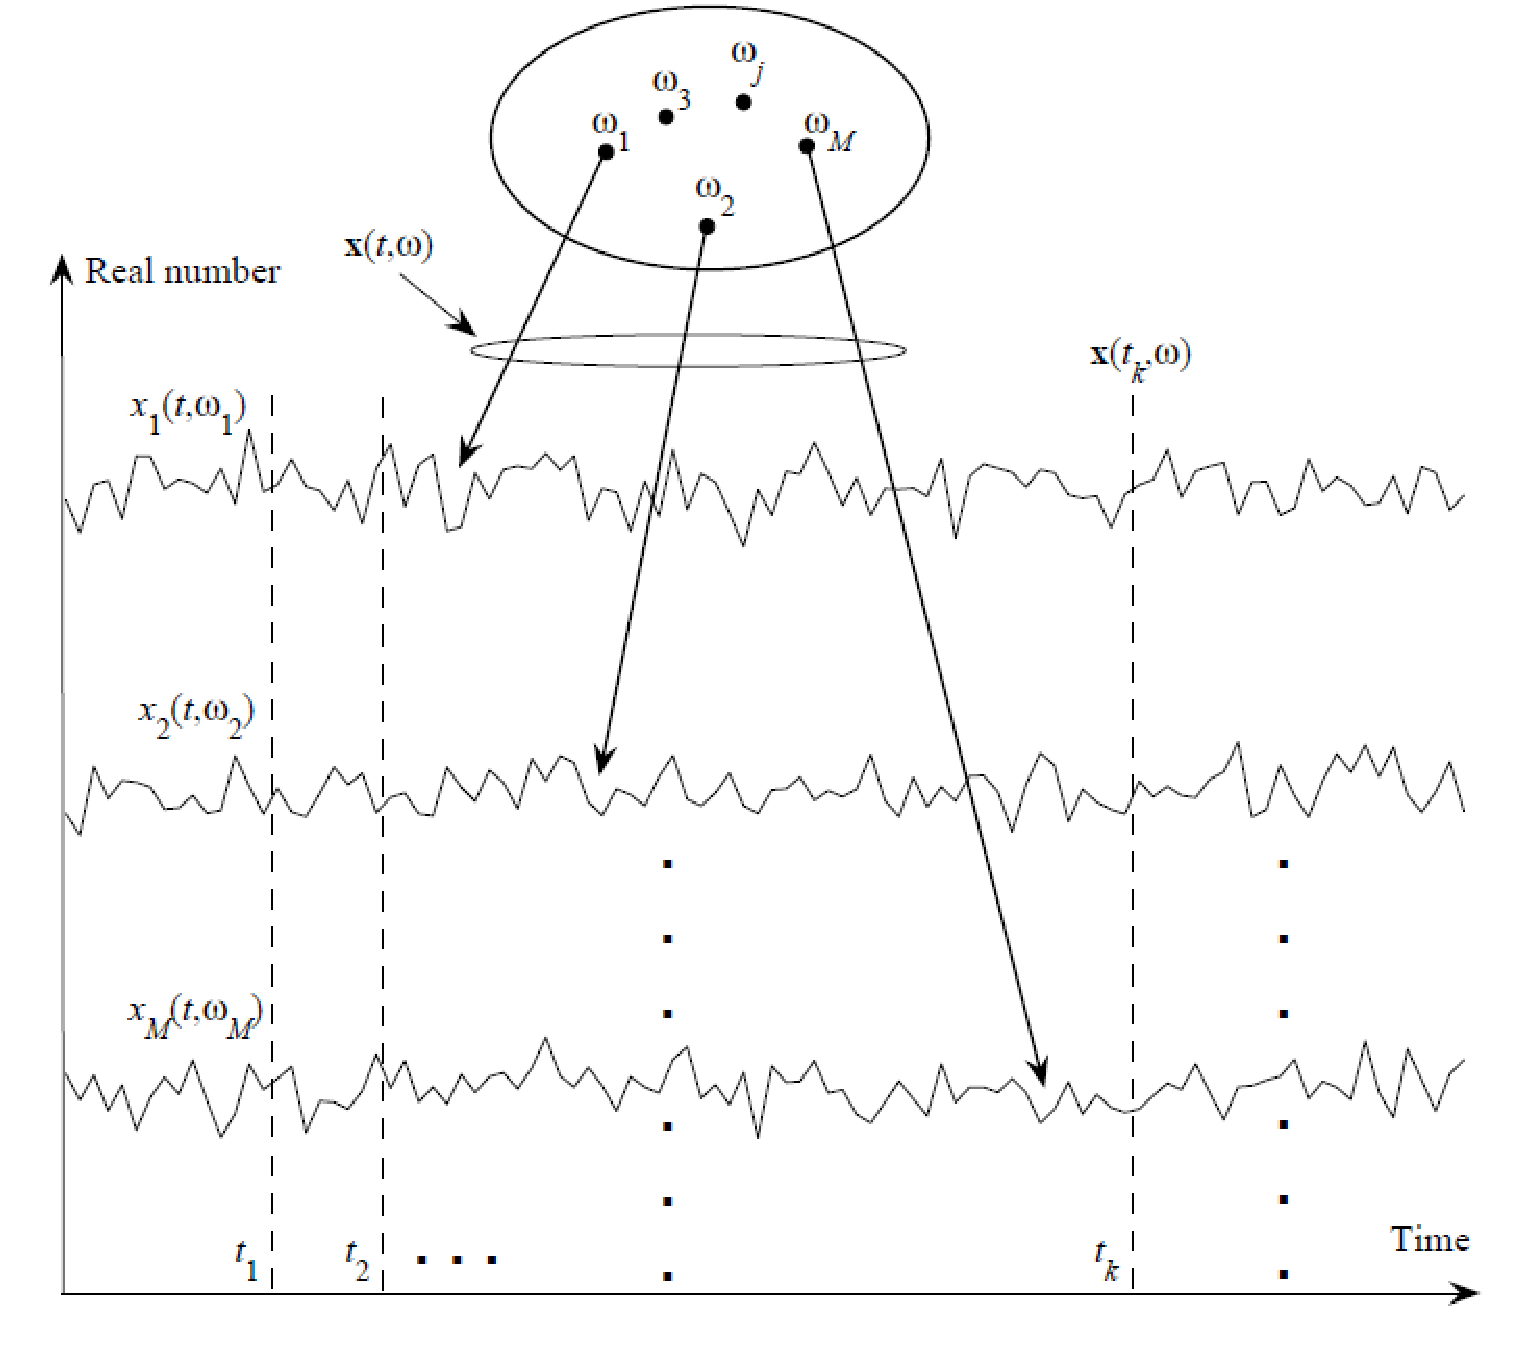
\includegraphics[width=0.5\columnwidth]{figs/fig22}
	  \end{center}
	\end{figure}
     Mapeamento de um espaço amostral em um \textit{conjunto de funções temporais}. 
\end{frame}

\begin{frame}
    \frametitle{Processos aleatórios - II}

    \begin{itemize}
     \item \textit{Ensemble}: conjunto de possíveis funções temporais denotado por $\vax(t)$, onde as funções temporais $x_1(t,\omega_1), x_2(t,\omega_2), x_3(t,\omega_3), \ldots$, são membros específicos do ensemble.
      \item Em um dado instante $t=t_k$, temos a variável aleatória $\vax(t_k)$.
      \item Em quaisquer dois instantes de tempo $t_1$ e $t_2$, temos duas diferentes variáveis aleatórias $\vax(t_1)$ e $\vax(t_2)$. Qualquer relação entre elas é descrita pela PDF conjunta $f_{\vax(t_1),\vax(t_2)}(x_1,x_2;t_1,t_2)$.
      \item Descrição completa do processo aleatório é determinada pela PDF conjunta $f_{\vax(t_1),\vax(t_2),\ldots,\vax(t_N)}(x_1,x_2,\ldots,x_N;t_1,t_2,\ldots,t_N)$.
      \item PDFs conjuntas mais importantes:
      \begin{itemize}
       \item Primeira ordem: $f_{\vax(t)}(x;t)$
	\item Segunda ordem: $f_{\vax(t_1),\vax(t_2)}(x_1,x_2;t_1,t_2)$
      \end{itemize}

    \end{itemize}

\end{frame}

\begin{frame}
    \frametitle{Exemplos de processos aleatórios - I}

    \begin{figure}[t]
	  \begin{center}
	    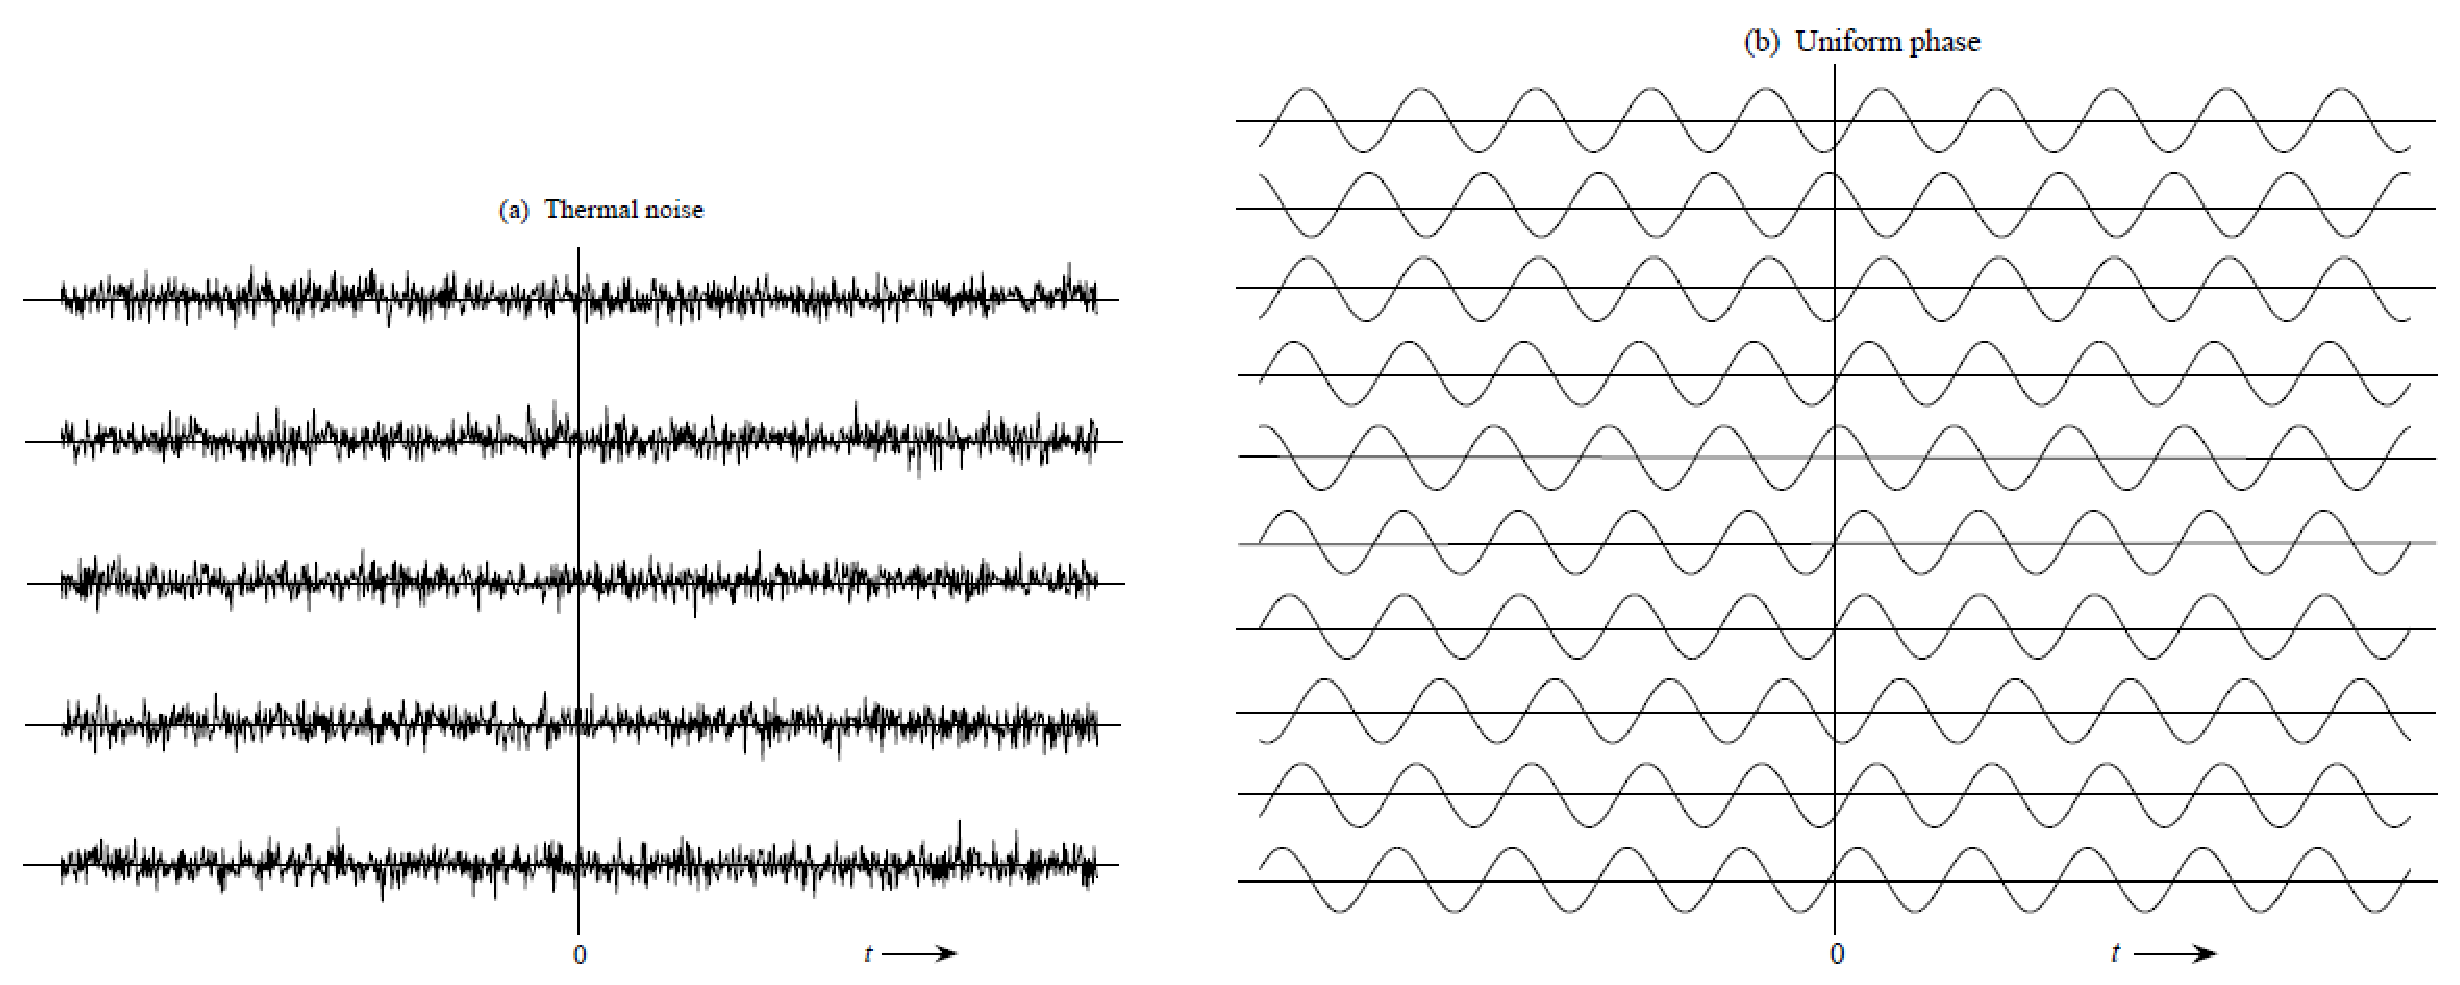
\includegraphics[width=0.95\columnwidth]{figs/fig23}
	  \end{center}
	\end{figure}
     
\end{frame}

\begin{frame}
    \frametitle{Exemplos de processos aleatórios - II}

    \begin{figure}[t]
	  \begin{center}
	    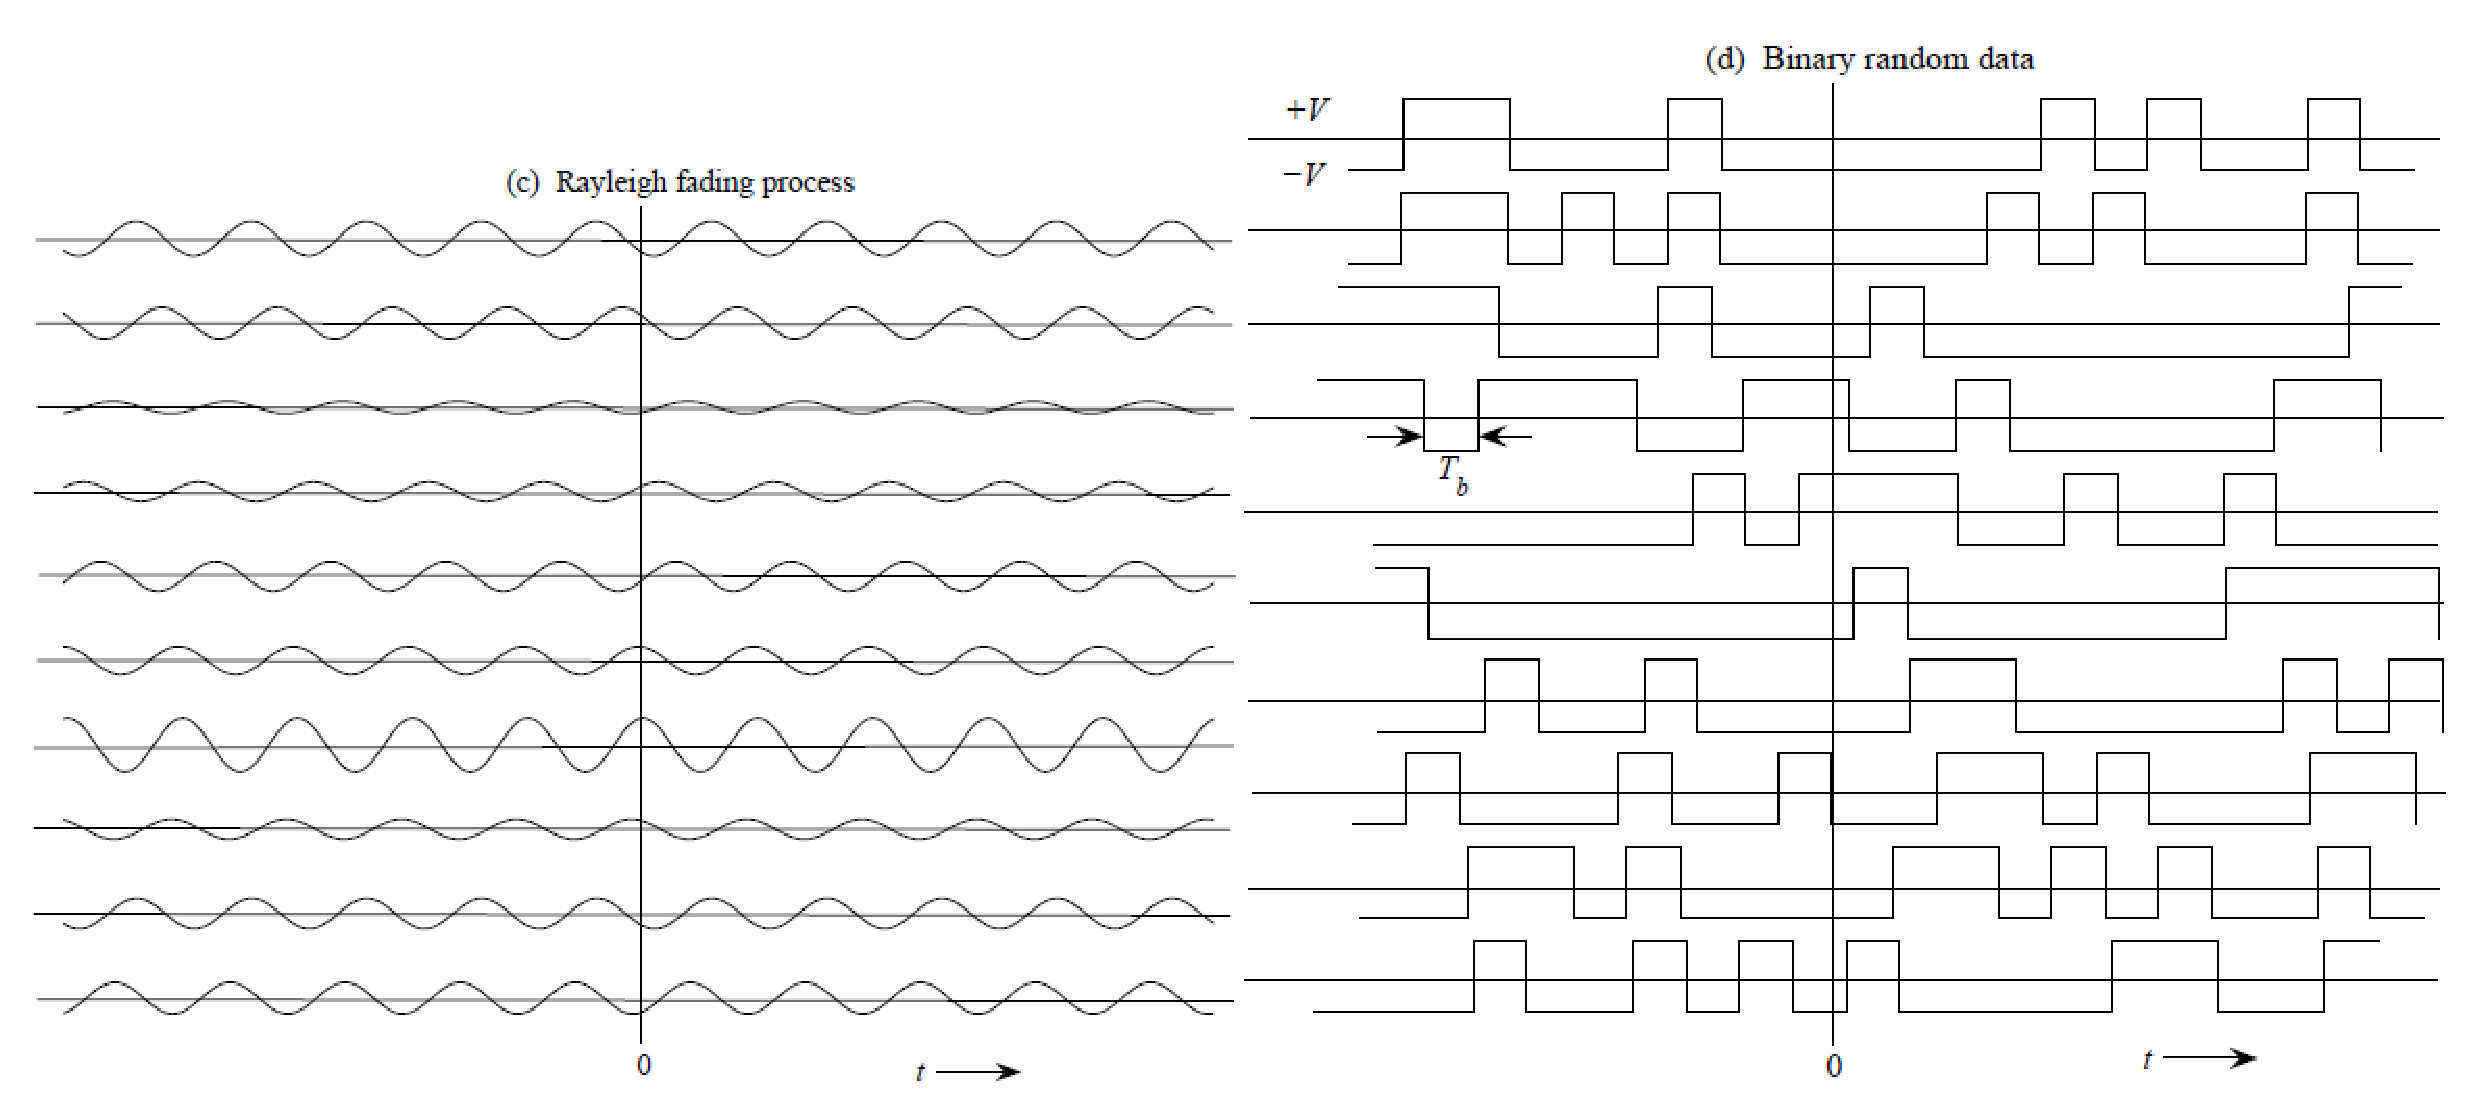
\includegraphics[width=0.95\columnwidth]{figs/fig24}
	  \end{center}
	\end{figure}
     
\end{frame}

\begin{frame}
    \frametitle{Classificação de processos aleatórios}

    \begin{itemize}
     \item Baseada na mudança das estatísticas com o tempo o processo pode ser: \textit{não-estacionário} ou \textit{estacionário}.
      \item Diferentes níveis de estacionariedade:
      \begin{itemize}
       \item Estritamente estacionário: a PDF conjunta de qualquer ordem é independente de um deslocamento temporal.
	\item Estacionariedade de ordem $N$: a PDF conjunta não depende do deslocamento temporal, mas depende de espaçamentos no tempo:
	\begin{align*}
	  f_{\vax(t_1),\vax(t_2),\ldots,\vax(t_N)}&(x_1,x_2,\ldots,x_n; t_1,t_2,\ldots,t_N) = \\
	  f_{\vax(t_1+t),\vax(t_2+t),\ldots,\vax(t_N+t)}&(x_1,x_2,\ldots,x_n; t_1+t,t_2+t,\ldots,t_N+t)
	\end{align*}
	\item Estacionariedade de primeira ordem:
	\begin{equation}
	  f_{\vax(t_1)}(x; t_1) = f_{\vax(t_1+t)}(x; t_1+t) = f_{\vax(t)}(x)
	\end{equation}
	\item Estacionariedade de segunda ordem:
	\begin{align*}
	  f_{\vax(t_1),\vax(t_2)}(x_1,x_2; t_1,t_2) &= f_{\vax(t_1+t),\vax(t_2+t)}(x_1,x_2; t_1+t, t_2+t) \\
	  &= f_{\vax(t_1),\vax(t_2)}(x_1,x_2; \tau), \qquad \tau = t_2 - t_1 \, .
	\end{align*}

      \end{itemize}

    \end{itemize}
     
\end{frame}

\begin{frame}
    \frametitle{Médias estatísticas ou momentos conjuntos}

    \begin{itemize}
     \item Considere $N$ variáveis aleatórias $\vax(t_1),\vax(t_2),\ldots,\vax(t_N)$. Os momentos conjuntos destas variáveis aleatórias são dados por:
    \begin{align*}
	E\{\vax^{k_1}(t_1),&\vax^{k_2}(t_2),\ldots,\vax^{k_N}(t_N)\} = \int_{x_1=-\infty}^{\infty} \cdots \int_{x_N=-\infty}^{\infty} \\
	&x_1^{k_1}x_2^{k_2} \cdots x_N^{k_N} f_{\vax(t_1),\vax(t_2),\ldots,\vax(t_N)}(x_1,x_2,\ldots,x_N; t_1,t_2,\ldots,t_N) \\
	& \mathrm{d}x_1 \mathrm{d}x_2 \ldots \mathrm{d}x_N \, ,
    \end{align*}

      para todos os inteiros $k_j \geq 1$ e $N \geq 1$.
      
      \item Vamos considerar somente os momentos de primeira e segunda ordem, i.e., $E\{\vax(t)\}$ (média), $E\{\vax^2(t)\}$ (valor quadrático médio) e $E\{\vax(t_1)\vax(t_2)\}$ (autocorrelação).
    \end{itemize}
     
\end{frame}

\begin{frame}
    \frametitle{Valor médio ou primeiro momento}

    \begin{itemize}
     \item O valor médio do processo em um tempo $t$ é:
      \begin{equation}
	  m_{\vax}(t) = E\{\vax(t)\} = \int_{-\infty}^{\infty} x f_{\vax(t)} (x;t) \mathrm{d}x \, .
      \end{equation}
      \item A média se dá ao longo do ensemble, e se a PDF varia com o tempo então o valor médio é uma função determinística do tempo.
      \item Se um processo é estacionário então a média é independente de $t$ ou uma constante.
\	\begin{equation}
 	 m_{\vax} = E\{\vax(t)\} = \int_{-\infty}^{\infty}x f_{\vax}(x) \mathrm{d}x \, . 
 	\end{equation}

    \end{itemize}
     
\end{frame}

\begin{frame}
    \frametitle{Valor quadrático médio ou segundo momento}

    \begin{itemize}
     \item O valor quadrático médio (MSV) é definido como:
      \begin{align*}
	  \mathrm{MSV}_{\vax}(t) &= E\{\vax^2(t)\} = \int_{-\infty}^{\infty} x^2 f_{\vax(t)}(x;t)\mathrm{d}x \quad &\textrm{(não-estac.)} \\
	  \mathrm{MSV}_{\vax} &= E\{\vax^2(t)\} = \int_{-\infty}^{\infty} x^2 f_{\vax}(x)\mathrm{d}x \quad &\textrm{(estac.)}
      \end{align*}
      \item O segundo momento central (ou variância) é:
      \begin{align*}
	  \sigma_{\vax}^2(t) &= E\{[\vax(t) - m_{\vax}(t)]^2\} = \mathrm{MSV}_{\vax}(t)  - m_{\vax}^2(t) \quad &\textrm{(não-estac.)} \\
	  \sigma_{\vax}^2 &= E\{[\vax(t) - m_{\vax}]^2\} = \mathrm{MSV}_{\vax}  - m_{\vax}^2 \quad &\textrm{(estac.)}
      \end{align*}

    \end{itemize}
     
\end{frame}

\begin{frame}
    \frametitle{Correlação}

    \begin{itemize}
     \item A função de autocorrelação descreve completamente a densidade espectral de potência do processo aleatório.
      \item Pode ser definida como a correlação entre duas variáveis aleatórias $\vax_1 = \vax(t_1)$ e $\vax_2 = \vax(t_2)$:
      \begin{small}
      \begin{align*}
	  R_{\vax}(t_1,t_2) = E\{\vax(t_1)\vax(t_2)\} = \int_{x_1=-\infty}^{\infty}\int_{x_2=-\infty}^{\infty} x_1 x_2 f_{\vax_1,\vax_2}(x_1,x_2;t_1,t_2)\mathrm{d}x_1\mathrm{d}x_2
      \end{align*}\end{small}
      \item Para um processo estacionário:
      \begin{small}
      \begin{align*}
	  R_{\vax}(\tau) = E\{\vax(t)\vax(t+\tau)\} = \int_{x_1=-\infty}^{\infty}\int_{x_2=-\infty}^{\infty} x_1 x_2 f_{\vax_1,\vax_2}(x_1,x_2;\tau)\mathrm{d}x_1\mathrm{d}x_2
      \end{align*}\end{small}
      \item Processo com \textit{estacionariedade no sentido amplo} (WSS): 
      \begin{itemize}
       \item $E\{\vax(t)\} = m_{\vax}$ para qualquer $t$, e $R_{\vax}(t_1,t_2) = R_{\vax}(\tau)$ para $\tau = t_2 - t_1$.
      \end{itemize}

    \end{itemize}
     
\end{frame}

\begin{frame}
    \frametitle{Propriedades da autocorrelação de um processo WSS}

    \begin{itemize}
     \item $R_{\vax}(\tau) = R_{\vax}(-\tau)$. É uma função par de $\tau$, uma vez que o mesmo conjunto de valores é mediado ao longo do ensemble, independente da direção de translação.
      \item $|R_{\vax}(\tau)| \leq R_{\vax}(0)$. O valor máximo sempre ocorre em $\tau = 0$. Além disso, $R_{\vax}(0)$ é o valor médio quadrático do processo aleatório.
      \item Se para um certo $\tau_0$ temos que $R_{\vax}(\tau_0) = R_{\vax}(0)$, então para qualquer inteiro $k$, $R_{\vax}(k\tau_0) = R_{\vax}(0)$.
      \item Se $m_{\vax} \neq 0$ então $R_{\vax}(\tau)$ possuirá uma componente constante igual a $m_{\vax}^2$.
      \item Funções de autocorrelação não podem ter uma forma arbitrária. A restrição da forma surge do fato de que a transformada de Fourier de uma função de autocorrelação deve ser maior ou igual a zero, i.e., $\mathcal{F}\{R_{\vax}(\tau)\} \geq 0$.
    \end{itemize}
     
\end{frame}

\begin{frame}
    \frametitle{Densidade espectral de potência de um processo aleatório - I}

    \begin{itemize}
     \item Um processo aleatório é um sinal de energia infinita, portanto não se pode tirar diretamente sua transformada de Fourier.
      \begin{figure}[t]
	  \begin{center}
	    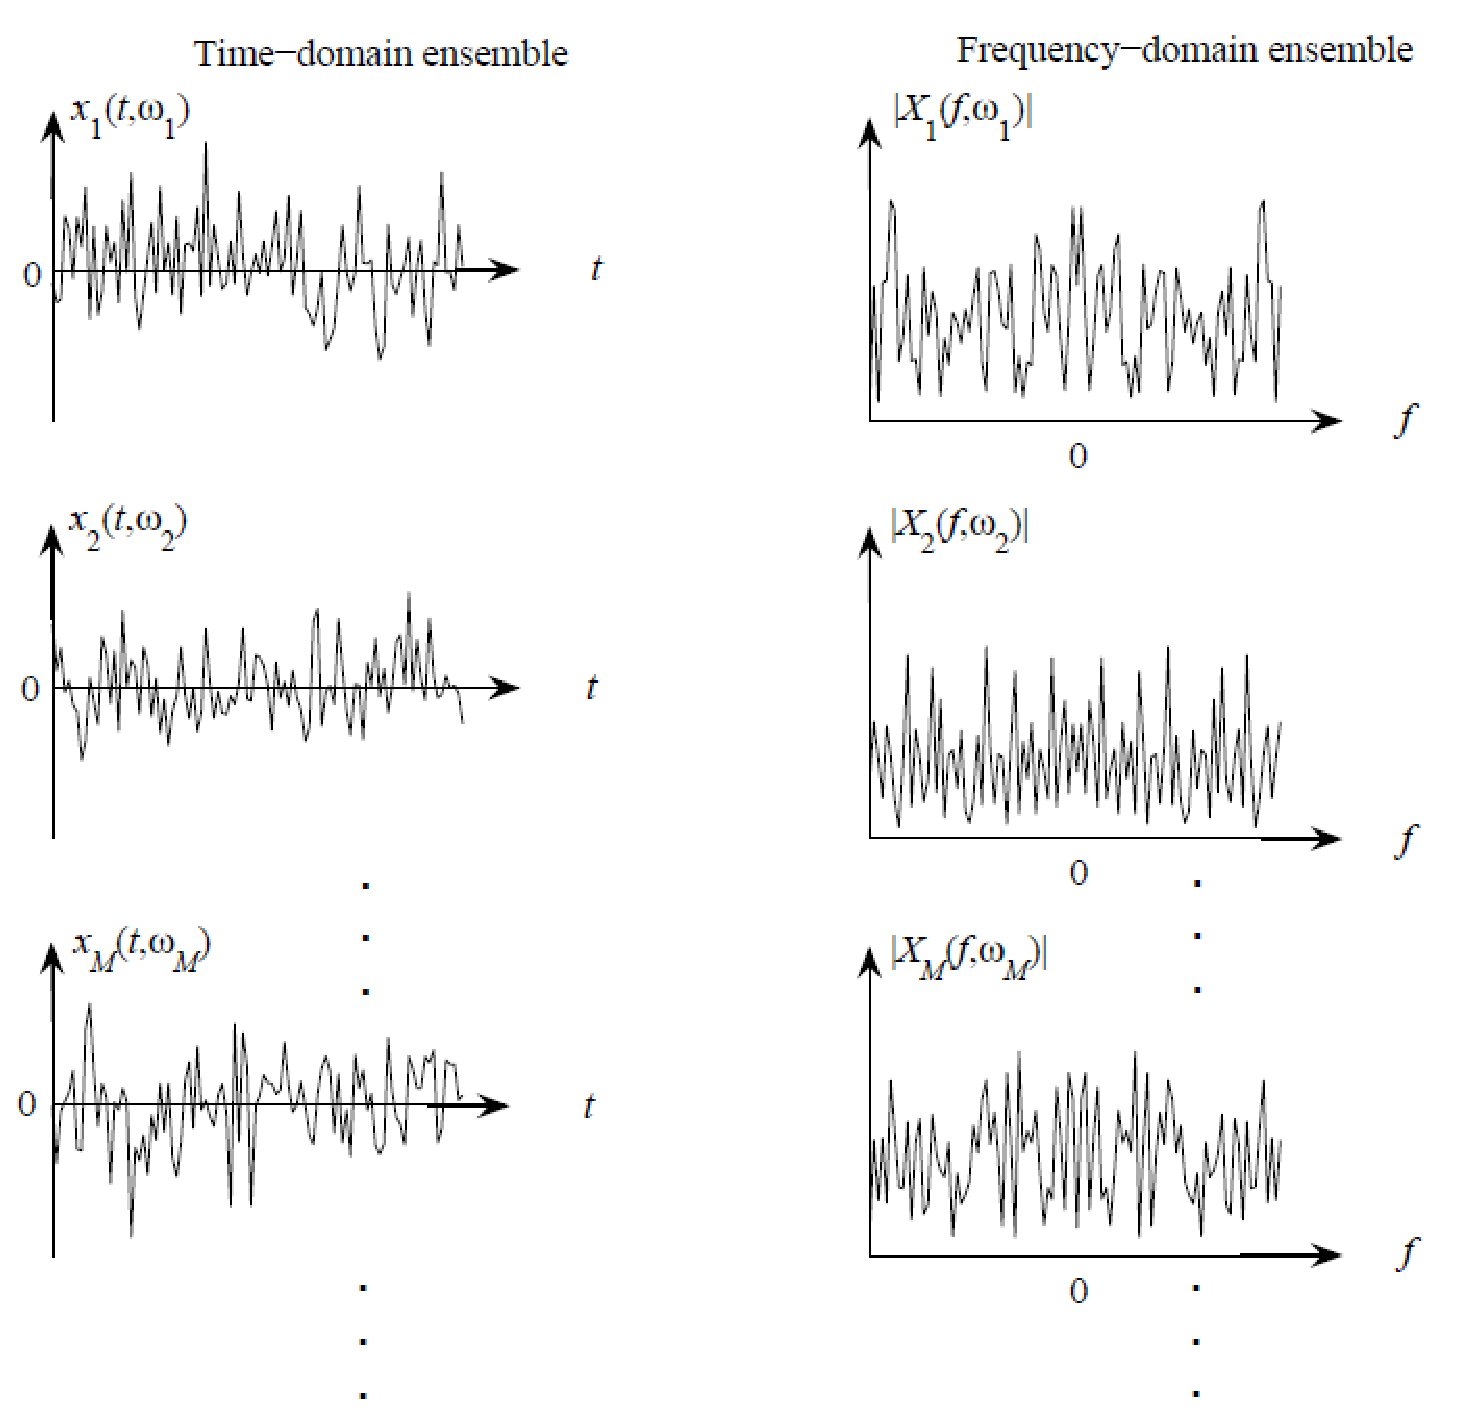
\includegraphics[width=0.55\columnwidth]{figs/fig25}
	  \end{center}
	\end{figure}
    \end{itemize}
     
\end{frame}

\begin{frame}
    \frametitle{Densidade espectral de potência de um processo aleatório - II}

    \begin{itemize}
     \item É necessário determinar como a potência média do processo se distribui na freqüência.
      \item Defina um processo truncado:

      \begin{equation}
	  \vax_T(t) = \begin{cases} \vax(t), \quad &-T \leq t \leq T \\ 0, \quad &\mathrm{c.c.} \end{cases} 
      \end{equation}
      \item Considere a transformada de Fourier do processo truncado:
      \begin{equation}
	  \mathbf{X}_T(f) = \int_{-\infty}^{\infty} \vax_T(t) \mathrm{e}^{-j2\pi ft} \mathrm{d}t \, .
      \end{equation}
      \item Medie a energia sobre o tempo total, $2T$:
      \begin{equation}
	  \mathbf{P} = \frac{1}{2T} \int_{-T}^T \vax_T^2(t)\mathrm{d}t = \frac{1}{2T} \int_{-\infty}^{\infty} |\mathbf{X}_T(f)|^2 \mathrm{d}f \quad \mathrm{(Watts)}
      \end{equation}

    \end{itemize}
          
\end{frame}

\begin{frame}
    \frametitle{Densidade espectral de potência de um processo aleatório - III}

    \begin{itemize}
     \item Encontre o valor médio de $\mathbf{P}$:
      \begin{equation}
	  E\{\mathbf{P}\} = E\left\{\frac{1}{2T} \int_{-T}^T \vax_T^2(t) \mathrm{d}t \right\} = E\left\{\frac{1}{2T} \int_{-\infty}^{\infty} |\mathbf{X}_T(f)|^2 \mathrm{d}f \right\}
      \end{equation}
      \item Toma-se o limite quando o período tende a infinito:
      \begin{equation}
	  \lim_{T \rightarrow \infty} \frac{1}{2T} \int_{-T}^T E\{\vax_T^2(t)\} \mathrm{d}t = \lim_{T \rightarrow \infty} \frac{1}{2T} \int_{-\infty}^{\infty} E\left\{ |\mathbf{X}_T(f)|^2 \right\} \mathrm{d}f \, .
      \end{equation}
      \item Segue que:
      \begin{equation}
	  \mathrm{MSV}_{\vax} = \int_{-\infty}^{\infty} \lim_{T \rightarrow \infty} \frac{E\left\{ |\mathbf{X}_T(f)|^2 \right\}}{2T}  \mathrm{d}f \quad \mathrm{(Watts)}
      \end{equation}

    \end{itemize}
          
\end{frame}

\begin{frame}
    \frametitle{Densidade espectral de potência de um processo aleatório - IV}

    \begin{itemize}
     \item Finalmente a \textit{densidade espectral de potência} é dada por:
      \begin{equation}
	  S_{\vax}(f) = \lim_{T \rightarrow \infty}\frac{E\left\{ |\mathbf{X}_T(f)|^2 \right\}}{2T} \quad \mathrm{(Watts/Hz)}
      \end{equation}
      \item Pode-se mostrar que a densidade espectral de potência e a função de autocorrelação formam um \textit{par da transformada de Fourier}:
      \begin{equation}
	  R_{\vax}(\tau) \longleftrightarrow S_{\vax}(f) = \int_{\tau = -\infty}^{\infty} R_{\vax}(\tau)\mathrm{e}^{-j2\pi f\tau}\mathrm{d}\tau \,.
      \end{equation}

    \end{itemize}
          
\end{frame}
 
\begin{frame}
    \frametitle{Média temporal e ergodicidade}

    \begin{itemize}
     \item Um processo é \textit{ergódico} quando qualquer membro do ensemble exibe o mesmo comportamento estatístico que todo o ensemble.
      \item Todas as médias temporais em um dado membro do ensemble são iguais à correspondente média do ensemble:
      \begin{equation}
	  E\{\vax^n (t) \} = \int_{-\infty}^{\infty} x^n f_{\vax}(x)\mathrm{d}x
      \end{equation}
      \item Em um processo ergódico: para medir diversas médias estatísticas, basta olhar para uma única realização do processo e encontrar a média temporal correspondente.
      \item Para um processo ser ergódico ele tem que ser estacionário. O reverso não é verdadeiro.

    \end{itemize}
          
\end{frame}

\begin{frame}
    \frametitle{Processos aleatórios e sistemas LTI}

    \begin{figure}[t]
	  \begin{center}
	    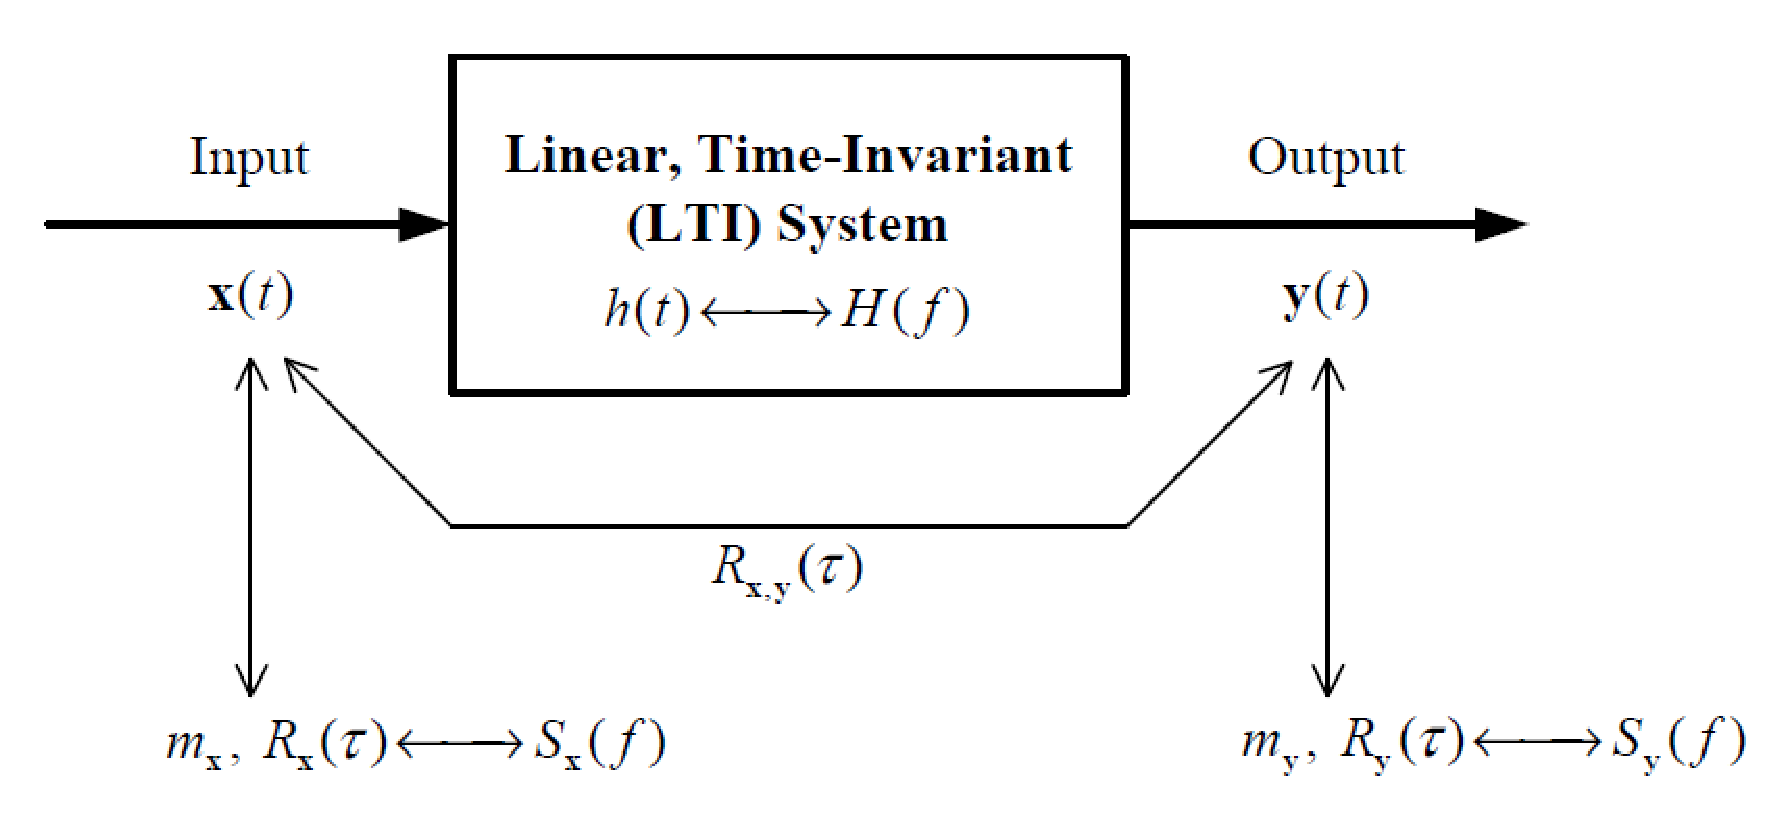
\includegraphics[width=0.7\columnwidth]{figs/fig26}
	  \end{center}
	\end{figure}
          
    \begin{align}
	  m_{\vay} &=  E\{\vay(t)\} = E\left\{ \int_{-\infty}^{\infty} h(\lambda)\vax(t-\lambda)\mathrm{d}\lambda \right\} = m_{\vax} H(0) \\
	  S_{\vay}(f) &= |H(f)|^2 S_{\vax}(f) \\
	  R_{\vay}(\tau) &= h(\tau) * h(-\tau) * R_{\vax}(\tau)
    \end{align}


\end{frame}


% \part{Caracterização de sinais e sistemas de comunicação}
% \lecture{Caracterização de Sinais e Sistemas}{lec_carac}

\begin{frame}
	\begin{block}{\centering\large\bfseries Parte 2}
		\centering\large\insertpart
	\end{block}
\end{frame}


\section{Introdução}

\begin{frame}
	\frametitle{Introduçao}

	\begin{itemize}
	 \item Sinais podem ser caracterizados como:
	  \begin{itemize}
	   \item Aleatório vs. determinístico, discreto vs. contínuo no tempo, amplitude discreta vs. contínua, passa-baixa vs. passa-faixa, energia finita vs. infinita, potência média finita vs. infinita, etc.
	  \end{itemize}
	  \item Neste capítulo:
	  \begin{itemize}
	   \item Caracterização de sinais e sistemas comumente encontrados na transmissão de informação digital sobre um canal de comunicação.
	   \item Representação de várias formas de sinais modulados digitalmente e suas características espectrais.
	  \end{itemize}
	\end{itemize}

\end{frame}


\section{Representação de sinais e sistemas em banda passante}

\begin{frame}
	\frametitle{Representação de sinais e sistemas em banda passante}

	\begin{itemize}
	 \item Transmissão de sinais digitais $\Rightarrow$ modulação de portadora
	 \item Canal limitado em largura de banda: 
	\begin{itemize}
	 \item Double sideband (DSB): intervalo de frequências centradas em torno da portadora
	 \item Single sideband (SSB): intervalo de frequências adjacentes à portadora
	 \end{itemize}
	\item Sinais e sistemas de banda estreita (narrowband)
	\begin{itemize}
	 \item Largura de banda muito menor que a frequência da portadora
	 \end{itemize}
	  \item Transmissão e recepção de sinais em banda passante:
	\begin{itemize}
	 \item Envolve translações de frequência
	 \end{itemize}
	 \item Sinais e canais passa-baixa equivalentes:
	\begin{itemize}
	 \item Não há perda de generalidade
	  \item Conveniência matemática
	  \item Independentes da frequência de portadora e bandas de canais
	 \end{itemize}
	\end{itemize}

\end{frame}

\begin{frame}
	\frametitle{Representação de sinais em banda passante}

	\begin{itemize}
	 \item Sinal $s(t)$ com conteúdo em frequência concentrado em uma banda estreita de frequências em torno de $f_c$
	\end{itemize}
	\begin{figure}[t]
	  \begin{center}
	    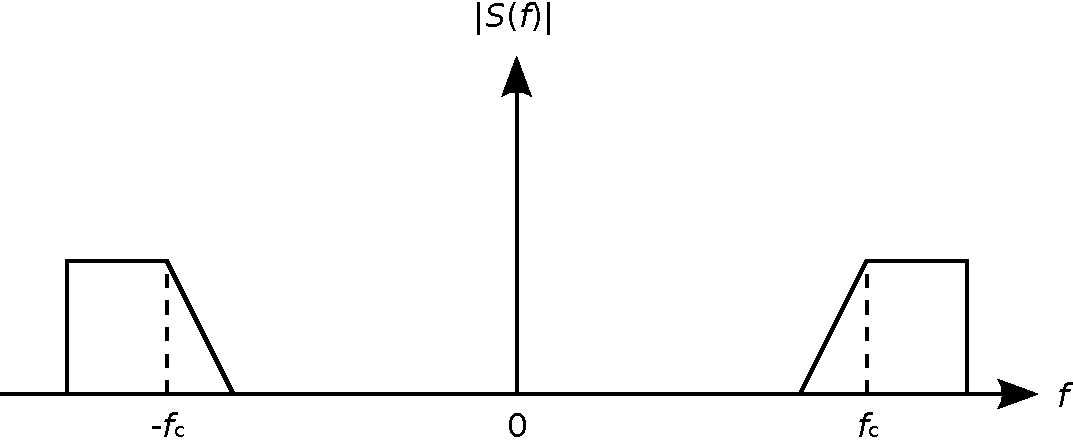
\includegraphics[width=0.5\columnwidth]{figs/4-1-1}
	  \end{center}
	\end{figure}
	\begin{itemize}
	 \item Sinal contendo as frequências positivas:
	\end{itemize}
	\begin{align*}
	      S_+(f) &= 2u(f)S(f) \\
	      s_+(t) &= \int_{-\infty}^{\infty}S_+(f)e^{j2\pi ft}df \\
	      &= F^{-1}[2u(f)] \ast F^{-1}[S(f)]
	\end{align*}

\end{frame}

\begin{frame}
	\frametitle{Representação de sinais em banda passante}

	\begin{itemize}
	 \item $s_+(t)$ é o sinal analítico ou pré-envoltória de $s(t)$
	 \item Considerando que $F^{-1}[S(f)] = s(t)$ e $F^{-1}[2u(f)] = \delta(t) + j/\pi t$
	\end{itemize}
	\begin{align*}
	    s_+(t) &= \left[ \delta(t) + \frac{j}{\pi t} \right] \ast s(t) \\
		  &= s(t) + j \underbrace{\frac{1}{\pi t}\ast s(t)}_{\hat{s}(t)}
	\end{align*}
	\begin{itemize}
	 \item $\hat{s}(t)$ pode ser visto como a saída do filtro de resposta ao impulso $h(t) = 1/\pi t$ quando excitado por $s(t)$. Transformada de Hilbert:
	\end{itemize}
	\begin{align*}
	    H(f) = \int_{-\infty}^{\infty} h(t) e^{-j2\pi ft}dt = \frac{1}{\pi} \int_{-\infty}^{\infty} \frac{1}{t} e^{-j2\pi ft}dt = \begin{cases} -j & f>0 \\ 0 & f = 0 \\ j & f < 0 \end{cases}
	\end{align*}
\end{frame}

\begin{frame}
	\frametitle{Representação de sinais em banda passante}

	\begin{itemize}
	 \item Efeito: deslocamento de fase de 90$^\mathrm{o}$ para todas as frequências de $s(t)$
	  \item Equivalente passa-baixa de $S_+(f)$: $S_l(f) = S_+(f+f_c)$
	  \item No domínio do tempo temos
	\end{itemize}
	\begin{align*}
	      s_l(t) &= s_+(t) e^{-j2\pi f_c t} = [s(t) + j \hat{s}(t)]e^{-j2\pi f_c t}
	\end{align*}
	\begin{itemize}
	 \item Considerando que $s_l(t) = x(t) + jy(t)$, podemos isolar $s(t)$ e $\hat{s}(t)$ como função das componentes do equivalente passa-baixa:
	\end{itemize}
	\begin{align*}
	      s(t) + j \hat{s}(t) &= s_l(t) e^{j2\pi f_c t} = [x(t) + jy(t)] e^{j2\pi f_c t} \\
	      s(t) &= x(t) \cos 2\pi f_c t - y(t) \sin 2\pi f_c t \\
	      \hat{s}(t) &= x(t) \sin 2\pi f_c t + y(t) \cos 2\pi f_c t \\
	\end{align*}

\end{frame}

\begin{frame}
	\frametitle{Representação de sinais em banda passante}

	\begin{itemize}
	 \item $x(t)$ e $y(t)$: componentes em quadratura do sinal em banda passante
	  \item $s_l(t)$: envoltória complexa do sinal real $s(t)$
	  \item Outras representações para o sinal em banda passante:
	\end{itemize}
	\begin{align*}
	    s(t) &= \mathrm{Re}\{[x(t) + jy(t)]e^{j2\pi f_c t}\} = \mathrm{Re}\{s_l(t) e^{j2\pi f_c t}\} \\
	    s(t) &= \mathrm{Re}\{a(t) e^{j[2\pi f_c t + \theta(t)]}\} = a(t) \cos [ 2\pi f_c t + \theta(t) ] \\
	\end{align*}
	\begin{itemize}
	 \item $a(t)$ e $\theta(t)$ são a envoltória e fase do sinal em banda passante
	 \item Temos que $s_l(t) = a(t) e^{j\theta(t)}$, $a(t) = \sqrt{x^2(t) + y^2(t)}$ e $\theta(t) = \tan^{-1} [y(t)/x(t)]$
	\end{itemize}

\end{frame}

\begin{frame}
	\frametitle{Representação de sinais em banda passante}

	\begin{itemize}
	 \item Calculando a transformada de Fourier de $s(t)$:
	\end{itemize}
	\begin{align*}
	    S(f) &= \int_{-\infty}^{\infty} s(t) e^{-j2\pi f t} dt = \int_{-\infty}^{\infty} \{ \mathrm{Re}[s_l(t) e^{j2\pi f_c t}] \} e^{-j2\pi f t} dt \\
	    &= \frac{1}{2} \int_{-\infty}^{\infty} [ s_l(t) e^{j2\pi f_c t} + s_l^*(t) e^{-j2\pi f_c t} ] e^{-j2\pi f t} dt \\
	    &= \frac{1}{2} [ S_l(f -f_c) + S_l^*(-f -f_c) ]
	\end{align*}
	\begin{itemize}
	 \item Relação básica entre o espectro do sinal equivalente passa-baixa e o espectro do sinal em banda passante
	\end{itemize}

\end{frame}

\begin{frame}
	\frametitle{Representação de sinais em banda passante}

	\begin{itemize}
	 \item Energia do sinal:
	\end{itemize}
	\begin{align*}
	    \mathcal{E} &= \int_{-\infty}^{\infty} s^2(t) dt = \int_{-\infty}^{\infty} \{ \mathrm{Re}[s_l(t)e^{j2\pi f_c t}] \}^2 dt \\
	    &= \frac{1}{2} \int_{-\infty}^{\infty} |s_l(t)|^2 dt + \color{red}{\frac{1}{2} \int_{-\infty}^{\infty} |s_l(t)|^2 \cos [4\pi f_c t + 2\theta(t)] dt}
	\end{align*}
	\begin{itemize}
	  \item Assumindo que $s(t)$ possui banda estreita, tem-se que a segunda integral possui um valor muito menor que a primeira, podendo ser desconsiderada
	  \item Pode-se afirmar que a energia do sinal equivalente passa-baixa corresponde, na prática, à energia do sinal em banda passante
	\end{itemize}

\end{frame}

\begin{frame}
	\frametitle{Representação de sinais em banda passante}

	\begin{figure}[t]
	  \begin{center}
	    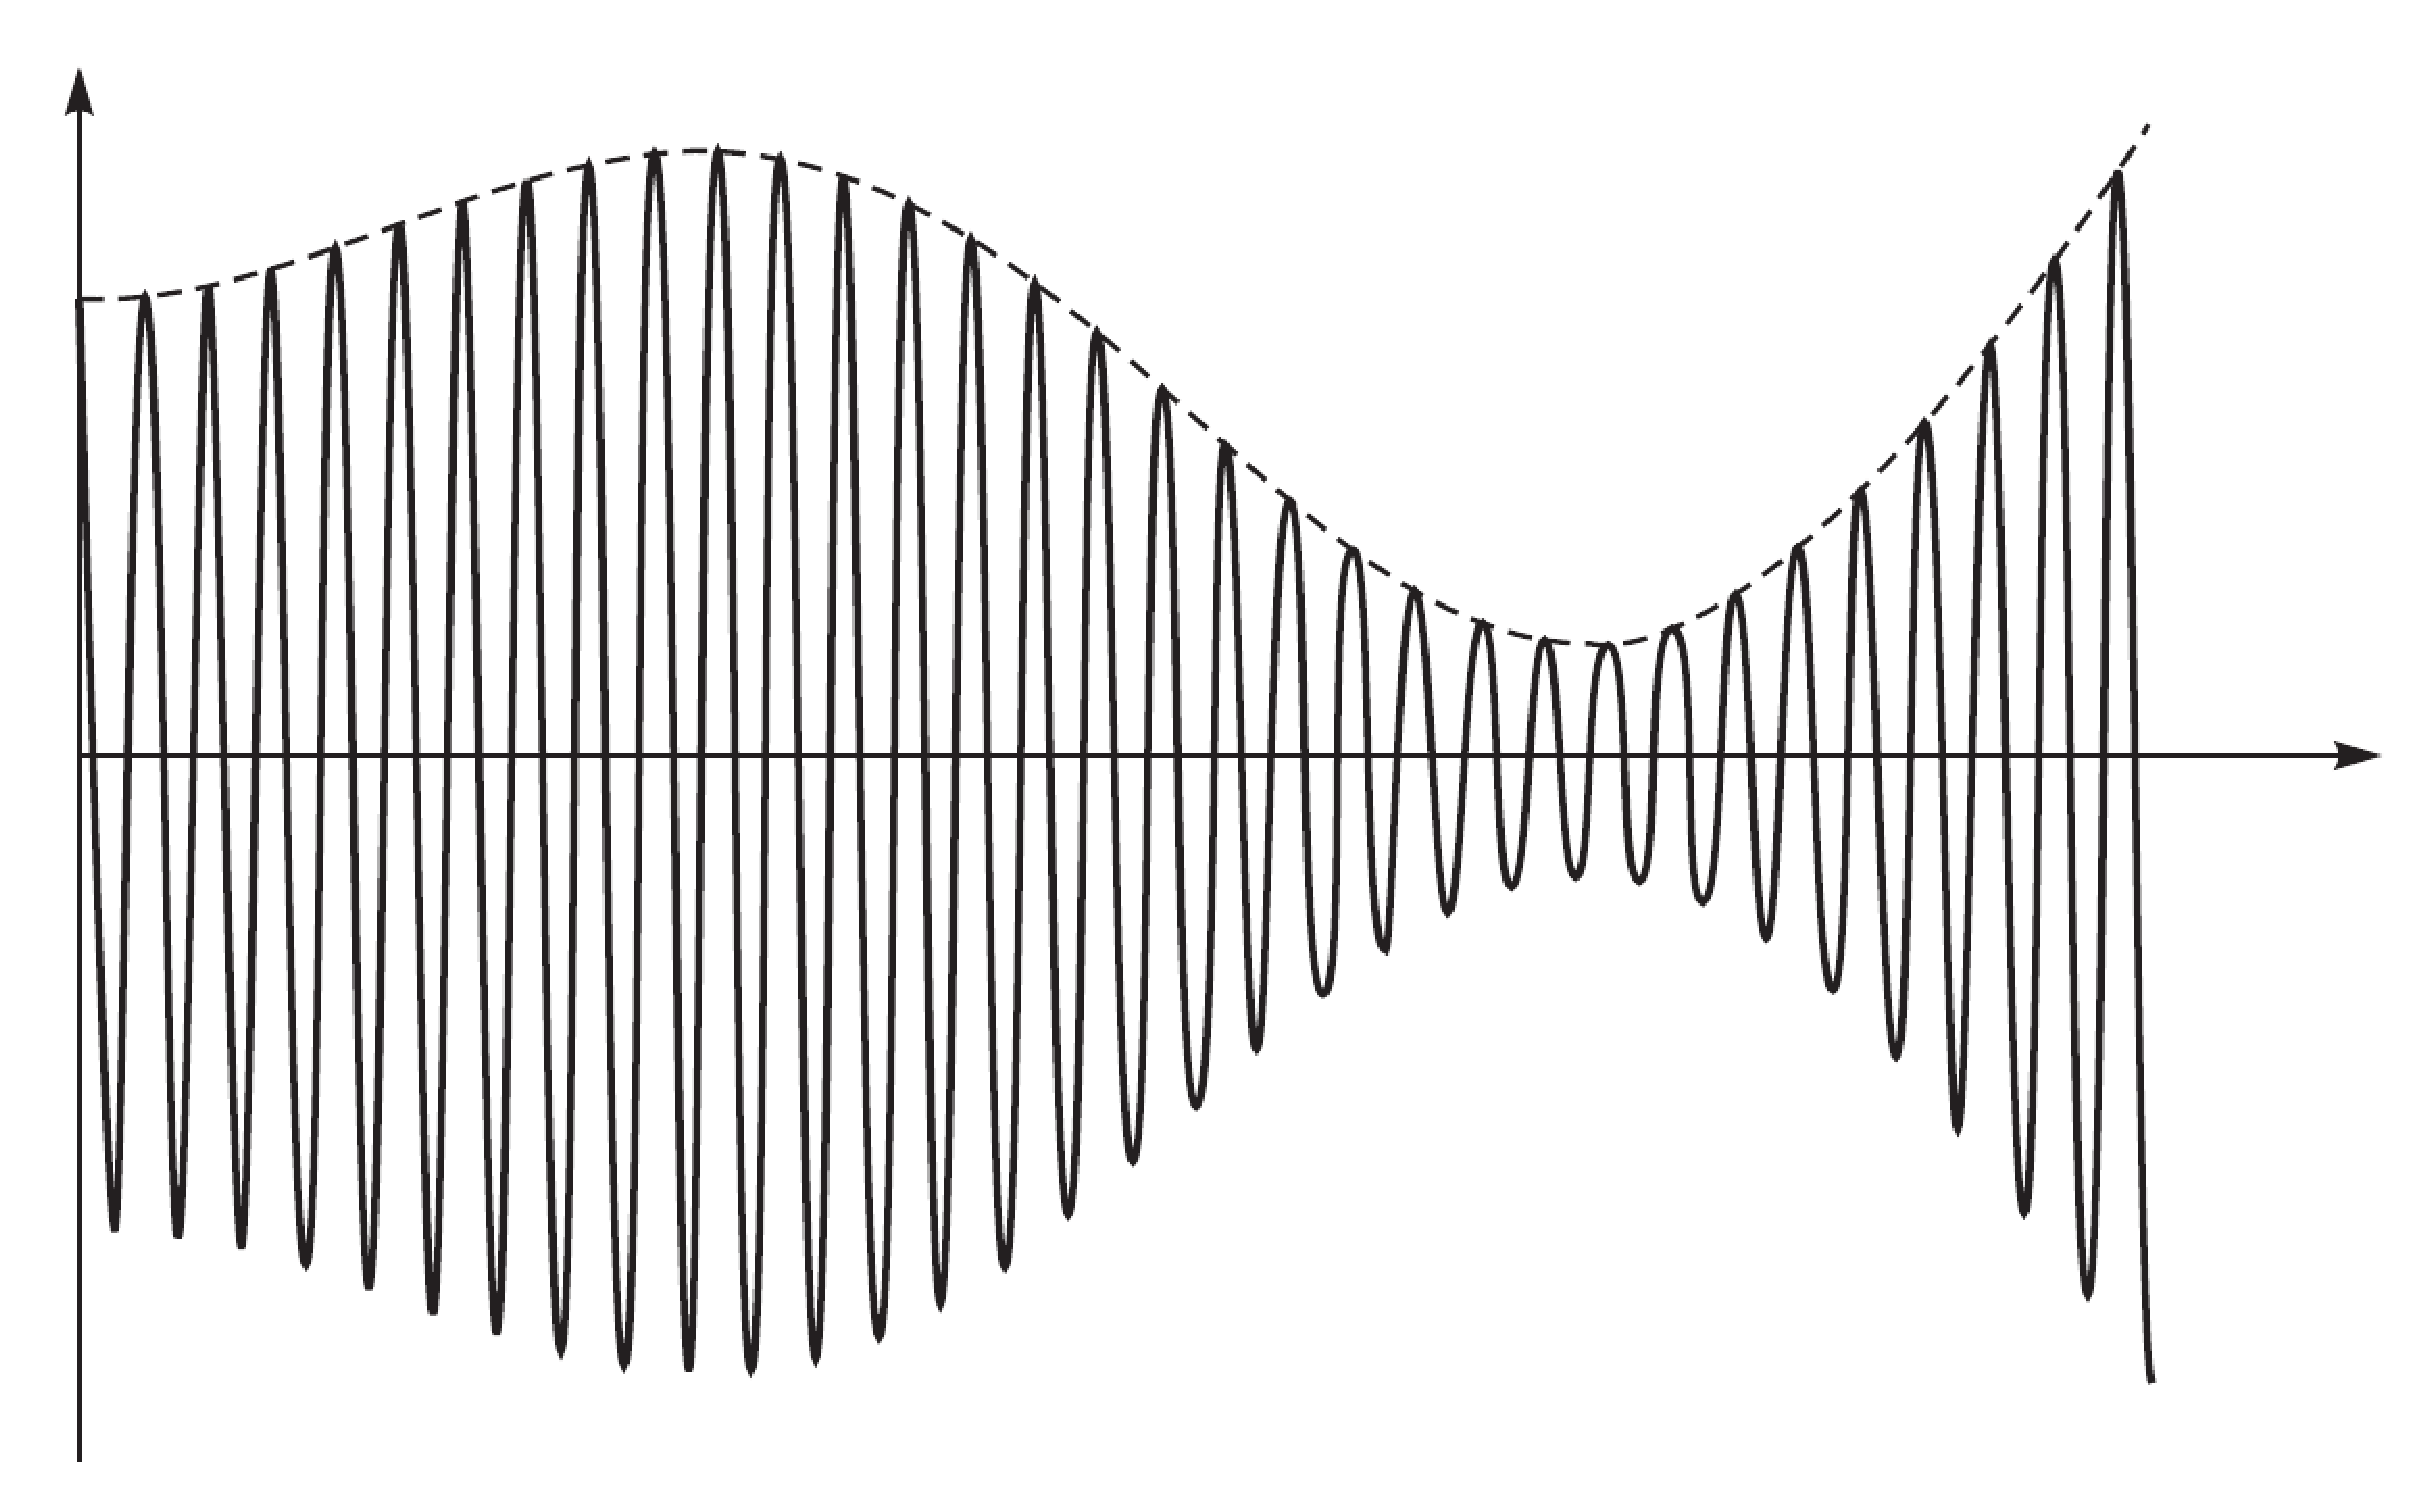
\includegraphics[width=0.5\columnwidth]{figs/fig02-01-04}
	  \end{center}
	\end{figure}

	\begin{itemize}
	  \item Para fins práticos pode-ser afirmar que, a energia do sinal em banda passante $s(t)$, expressa em termos do sinal equivalente passa-baixa $s_l(t)$, é dada por:
	\end{itemize}
	\begin{equation*}
	      \mathcal{E} = \frac{1}{2} \int_{\infty}^{\infty} |s_l(t)|^2 dt
	\end{equation*}


\end{frame}

\begin{frame}
	\frametitle{Representação de um sistema linear em banda passante}

	\begin{itemize}
	  \item Um filtro ou um sistema linear pode ser descrito por $h(t)$ ou $H(f)$.
	  \item Assumindo que $h(t)$ é real:
	  	\begin{equation*}
	      H^*(-f) = H(f)
	\end{equation*}
	  \item Considere que:
	\begin{align*}
	      H_l(f-f_c) &= \begin{cases}
				H(f) , &f > 0 \\
			        0, &f < 0 
	                    \end{cases} \\
	      H_l^*(-f-f_c) &= \begin{cases}
				0, &f > 0 \\
			        H^*(-f), &f < 0 
	                    \end{cases}
	\end{align*}
	 \item Então:
	\begin{equation*}
	    H(f) = H_l(f-f_c) + H_l^*(-f-f_c)
	\end{equation*}
	\end{itemize}


\end{frame}

\begin{frame}
	\frametitle{Resposta de um sistema em banda passante a um sinal em banda passante}

	\begin{itemize}
	  \item A resposta de um sistema em banda passante a um sinal de entrada em banda passante pode ser obtida a partir dos equivalentes passa-baixa do sinal de entrada e da resposta ao impulso do sistema.
	  \begin{figure}[t]
	  \begin{center}
	    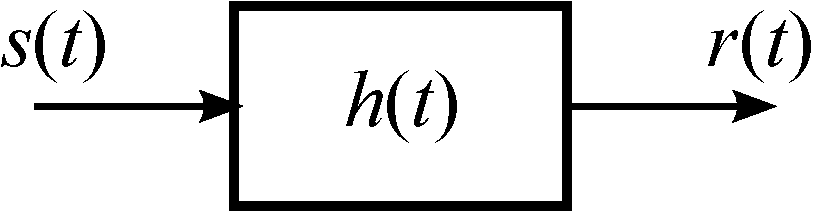
\includegraphics[width=0.3\columnwidth]{figs/system}
	  \end{center}
	\end{figure}
	  \item A saída do sistema também é um sinal em banda passante e pode ser representada por: $r(t) = \mathrm{Re}[r_l(t)e^{j2\pi f_c t}]$
	 \begin{small}\begin{align*}
	      R(f) &= S(f)H(f) \\
	      &= \frac{1}{2}[S_l(f-f_c) + S_l^*(-f-f_c)][H_l(f-f_c) + H_l^*(-f-f_c)] \\
	      &= \frac{1}{2}[S_l(f-f_c)H_l(f-f_c) + S_l^*(-f-f_c)H_l^*(-f-f_c)] \\
	      &= \frac{1}{2}[R_l(f-f_c) + R_l^*(-f-f_c)]
	\end{align*}	            \end{small}
	\end{itemize}


\end{frame}

\begin{frame}
	\frametitle{Representação de processos estocásticos estacionários em banda passante}

	\begin{itemize}
	  \item Representação é extendida para funções amostra de um processo estocástico estacionário em banda passante.
	  \item Derivação das relações entre as funções de correlação e o espectro de potência dos sinais em banda passante e do equivalente passa-baixa.
	  \item Processo estocástico do ruído
	  \begin{itemize}
	   \item $n(t)$: função amostra de um processo WSS com média zero e DEP $\Phi_{nn}(f)$
	   \item DEP limitada a um intervalo de frequências em torno de $f_c$
	   \item Processo em banda passante de banda estreita: largura da DEP $\gg f_c$
	   \item Representação do ruído:
	   \begin{align*}
		n(t) &= a(t)\cos[2\pi f_c t + \theta(t)] \\
		&= x(t)\cos 2\pi f_c t - y(t) \sin 2\pi f_c t \\
		&= \mathrm{Re}[z(t)e^{j2\pi f_c t}]
	   \end{align*}

	  \end{itemize}

	\end{itemize}

\end{frame}

\begin{frame}
	\frametitle{Representação de processos estocásticos estacionários em banda passante}

	\begin{itemize}
		\item Se $n(t)$ possui média zero, então $x(t)$ e $y(t)$ também têm média zero.
		\item A estacionariedade de $n(t)$ implica nas seguintes propriedades:
		\begin{align*}
			\phi_{xx}(\tau) &= \phi_{yy}(\tau) \\
			\phi_{xy}(\tau) &= -\phi_{yx}(\tau) 
		\end{align*}
		\item Função de autocorrelação do processo $n(t)$:
		\begin{equation*}
			\phi_{nn}(\tau) = \phi_{xx}(\tau)\cos 2\pi f_c \tau - \phi_{yx}(\tau)\sin 2\pi f_c \tau
		\end{equation*}
		\item Função de autocorrelação do processo equivalente passa-baixa $z(t) = x(t) + jy(t)$:
		\begin{align*}
			\phi_{zz}(\tau) &= \frac{1}{2} \expec[z^*(t) z(t+\tau)] = \phi_{xx}(\tau) + j\phi_{yx}(\tau) \\
			\phi_{nn}(\tau) &= \mathrm{Re}[\phi_{zz}(\tau)e^{j2\pi f_c \tau}]
		\end{align*}
	\end{itemize}

\end{frame}

\begin{frame}
	\frametitle{Representação de processos estocásticos estacionários em banda passante}

	\begin{itemize}
		\item Densidade espectral de potência do processo $n(t)$:
		\begin{small}\begin{equation*}
			\Phi_{nn}(f) = \int_{-\infty}^{\infty}\{\mathrm{Re}[\phi_{zz}(\tau)e^{j2\pi f_c \tau}]\}e^{-j2\pi f \tau} d\tau = \frac{1}{2}[\Phi_{zz}(f-f_c)+\Phi_{zz}(-f-f_c)]
		\end{equation*}		               \end{small}
 		\item Uma vez que $\phi_{zz}(\tau) = \phi_{zz}^*(-\tau)$,  então $\Phi_{zz}(f)$ é real.
		\item A partir das relações:
		\vspace{-0.1cm}\begin{align*}
			\phi_{xy}(\tau) &= -\phi_{yx}(\tau) \\
			\phi_{yx}(\tau) &= \phi_{xy}(-\tau)
		\end{align*}
 		\item Temos que $\phi_{xy}(\tau) = -\phi_{xy}(-\tau)$,  ou seja, $\phi_{xy}(\tau)$ é uma função ímpar.
		\item Consequentemente, $\phi_{xy}(0) = 0$, o que significa que $x(t)$ e $y(t)$ são descorrelacionados para $\tau=0$.
		\item Caso $\phi_{xy}(\tau) = 0$ para todo $\tau$,  então $\phi_{zz}(\tau)$ é real e $\Phi_{zz}(f) = \Phi_{zz}(-f)$.
	\end{itemize}

\end{frame}

\begin{frame}
	\frametitle{Representação de processos estocásticos estacionários em banda passante}

	\begin{itemize}
		\item Caso em que $n(t)$ é um processo Gaussiano:
		\begin{itemize}
			\item Componentes em quadratura $x(t)$ e $y(t+\tau)$ são conjuntamente Gaussianas.
			\item Para $\tau=0$ são independentes e possuem densidade conjunta:
			\begin{equation*}
				p(x,y) = \frac{1}{2\pi \sigma^2}e^{-(x^2+y^2)/2\sigma^2}
			\end{equation*}
			\item Onde $\sigma^2 = \phi_{xx}(0) = \phi_{yy}(0) = \phi_{nn}(0)$.
		\end{itemize}
	\end{itemize}

\end{frame}

\begin{frame}
	\frametitle{Representação de processos estocásticos estacionários em banda passante}

	\begin{itemize}
		\item Representação do ruído branco:
		\begin{itemize}
			\item DEP constante sobre todo o espectro de frequência.
			\item Ruído branco de banda estreita: assume-se que o ruído passou por um filtro e está limitado à banda do sinal.
			\item DEP e autocorrelação do equivalente passa-baixa $z(t)$:
			\begin{align*}
				\Phi_{zz}(f) &= \begin{cases}
							N_0 &\quad (|f| \leq B/2) \\
							0 &\quad (|f| > B/2)
				               \end{cases} \\
				\phi_{zz}(\tau) &= N_0 \frac{\sin \pi B \tau}{\pi\tau} \; ; \quad \lim_{B \to \infty} \phi_{zz}(\tau) = N_0\delta(\tau)
			\end{align*}
			\item Como a DEP é simétrica em torno de $f=0$, então $\phi_{yx}=0$ para todo $\tau$ e $\phi_{zz}(\tau)=\phi_{xx}(\tau)=\phi_{yy}(\tau)$.
			\item Ou seja, $x(t)$ e $y(t)$ são sempre descorrelacionados e as autocorrelações de $z(t)$,  $x(t)$ e $y(t)$ são iguais.
		\end{itemize}

	\end{itemize}

\end{frame}


%--------------------

\section{Representação em espaço de sinais}

\begin{frame}
	\frametitle{Conceitos de espaço vetorial}

	\begin{itemize}
	 \item Um vetor $\vv$ em um espaço $n$-dimensional é caracterizado por suas $n$ componentes $[v_1 \; v_2 \; \ldots \; v_n]$
	  \item Também pode ser representado como uma combinação linear de vetores unitários: $\vv = \sum\limits_{i=1}^n v_i \, \ve_i$, para $1 \leq i \leq n$
	  \item Onde $v_i$ é a projeção de $\vv$ em $\ve_i$
	  \item O produto interno de dois vetores $n$-dimensionais é dado por: $\vv_1 \cdot \vv_2 = \sum\limits_{i=1}^n v_{1i} \, v_{2i}$
	  \item Condição de ortogonalidade entre dois vetores: $\vv_1 \cdot \vv_2 = 0$
	  \item Um conjunto de $m$ vetores $\vv_k$, $1\leq k \leq m$, é ortogonal se: $\vv_i \cdot \vv_j = 0$ para todo $(i,j) \in \{1, \ldots, m\}$ e $i \neq j$
	\end{itemize}

\end{frame}


\begin{frame}
	\frametitle{Conceitos de espaço vetorial}

	\begin{itemize}
	 \item Norma de um vetor: $||\vv|| = (\vv \cdot \vv)^{1/2} = \sqrt{\sum\limits_{i=1}^n v_i^2}$
	  \item Conjunto de vetores ortonormais: conjunto de vetores ortogonais onde cada vetor possui norma unitária
	  \item Conjunto de vetores LI: nenhum vetor do conjunto pode ser expresso como uma combinação linear dos outros vetores
	  \item Desigualdade triangular: $||\vv_1 + \vv_2|| \leq ||\vv_1|| + ||\vv_2||$. Igualdade somente para $\vv_1$ e $\vv_2$ colineares, ou seja, $\vv_1 = a\vv_2$
	  \item Desigualdade de Cauchy-Schwarz: $|\vv_1 \cdot \vv_2| \leq ||\vv_1 || \; ||\vv_2 ||$. Igualdade somente para $\vv_1 = a\vv_2$
	  \item Norma ao quadrado da soma de vetores: $||\vv_1 + \vv_2||^2 = ||\vv_1||^2 + ||\vv_2||^2 + 2 \vv_1 \cdot \vv_2$
	  \item Se $\vv_1$ e $\vv_2$ são ortogonais, então $||\vv_1 + \vv_2||^2 = ||\vv_1||^2 + ||\vv_2||^2$
	\end{itemize}

\end{frame}

\begin{frame}
	\frametitle{Conceitos de espaço vetorial}

	\begin{itemize}
	 \item Transformação linear em um espaço $n$-dimensional: $\vv' = \mA \vv$
	  \item Caso particular em que $\vv' = \lambda \vv$ temos que: $\mA \vv = \lambda \vv$
 	  \item $\vv$ é chamado de autovetor da transformação e $\lambda$ é o autovalor correspondente
	  \item Procedimento de Gram-Schmidt: construção de um conjunto de vetores ortonormais a partir de um conjunto de vetores $n$-dimensionais $\vv_i$
	\end{itemize} \vspace{-0.4cm}
	\begin{align*}
	      \vu_1 &= \vv_1 / ||\vv_1|| \\
	      \vu_2' &= \vv_2 - (\vv_2 \cdot \vu_1)\vu_1 \quad , \qquad \vu_2 = \vu_2' / ||\vu_2'|| \\
	      \vu_3' &= \vv_3 - (\vv_3 \cdot \vu_1)\vu_1 - (\vv_3 \cdot \vu_2)\vu_2 \quad , \qquad \vu_3 = \vu_3' / ||\vu_3'|| \\
	      \ldots
	\end{align*} \vspace{-0.5cm}
	\begin{itemize} 
	 \item Obtém-se um conjunto de $n_1$ vetores onde, em geral, $n_1 \leq n$
	\end{itemize}

\end{frame}

\begin{frame}
	\frametitle{Conceitos de espaço de sinais}

	\begin{itemize}
	  \item Analogia entre vetores e conjunto de sinais definidos em intervalo $[a,b]$
	  \item Sejam os sinais complexos $x_1(t)$ e $x_2(t)$, o seu produto interno é: $<x_1(t),x_2(t)> = \int_a^b x_1(t) x_2^*(t) dt$
	  \item A norma de um sinal é definida como: $||x(t)|| = \left( \int_a^b |x(t)|^2 dt \right)^{1/2}$
	  \item Definições de conjunto ortonormal e independência linear análogas ao caso vetorial
	  \item Desigualdade triangular: $||x_1(t) + x_2(t)|| \leq ||x_1(t)|| + ||x_2(t)||$
	  \item Desigualdade de Cauchy-Schwarz: 
	  \begin{equation*}
		    \left|\int_a^b x_1(t) x_2^*(t) dt \right| \leq \left|\int_a^b |x_1(t)|^2 dt \right|^{1/2} \left|\int_a^b |x_2(t)|^2 dt\right|^{1/2}
	  \end{equation*}
	\end{itemize}

\end{frame}

\begin{frame}
	\frametitle{Expansão ortogonal de sinais}

	\begin{itemize}
		\item Sinal $s(t)$ determinístico, real e de energia finita: $\mathcal{E}_s = \int_{-\infty}^{\infty}[s(t)]^2 dt$
		\item Conjunto de funções ortonormais $\{ f_n(t), n=1, 2, \ldots, N\}$ tal que
		\begin{equation*}
			\int_{-\infty}^{\infty} f_n(t)f_m(t) dt = \begin{cases}
									0 &\quad (m\neq n) \\
									1 &\quad (m=n)
			                                          \end{cases}
		\end{equation*}
		\item O sinal $s(t)$ pode ser aproximado por uma combinação linear destas funções:
		\begin{equation*}
			\hat{s}(t) = \sum_{k=1}^{K} s_k f_k(t)
		\end{equation*}
		\item Onde $\{s_k, 1\leq k \leq K\}$ são os coeficientes na aproximação de $s(t)$, sendo o erro de aproximação dado por:
		\begin{equation*}
			e(t) = s(t) - \hat{s}(t)
		\end{equation*}
	\end{itemize}

\end{frame}

\begin{frame}
	\frametitle{Expansão ortogonal de sinais}

	\begin{itemize}
		\item Energia do erro de aproximação:
		\begin{small}\begin{equation*}
			\mathcal{E}_e = \int_{-\infty}^{\infty}[s(t)-\hat{s}(t)]^2 dt = \int_{-\infty}^{\infty}\left[ s(t) - \sum_{k=1}^{K} s_k f_k(t) \right]^2 dt
		\end{equation*}		               \end{small}
		\item Coeficientes ótimos que minimizam a energia do erro podem ser obtidos ao resolver o problema de otimização.
		\item Forma alternativa de encontrar a solução: resultado da teoria da estimação baseado no critério do erro médio quadrático.
		\item O mínimo de $\mathcal{E}_e$ com respeito a $\{s_k\}$ é obtido quando o erro é ortogonal a cada uma das funções da expansão em série, ou seja,
		\begin{small}\begin{equation*}
			\int_{-\infty}^{\infty}\left[ s(t) - \sum_{k=1}^{K} s_k f_k(t) \right]f_n(t) dt = 0,  \quad n=1, 2, \ldots, K
		\end{equation*}		               \end{small}
		\item Como as funções $\{f_n(t)\}$ são ortonormais então temos que:
		\begin{small}\begin{equation*}
			s_n = \int_{-\infty}^{\infty} s(t) f_n(t) dt,  \quad n=1, 2, \ldots, K
		\end{equation*}		               \end{small}
	\end{itemize}
\end{frame}

\begin{frame}
	\frametitle{Expansão ortogonal de sinais}

	\begin{itemize}
		\item Os coeficientes são obtidos ao se projetar $s(t)$ em cada função $\{f_n(t)\}$.
		\item $\hat{s}(t)$ é a projeção de $s(t)$ sobre o espaço de sinal $K$-dimensional definido pelas funções $\{f_n(t)\}$.
		\item O erro quadrático médio de aproximação é dado por:
		\begin{small}\begin{equation*}
			\mathcal{E}_{\text{min}} = \int_{-\infty}^{\infty} e(t) s(t) dt = \int_{-\infty}^{\infty} [s(t)]^2 dt - \int_{-\infty}^{\infty} \sum_{k=1}^{K} s_k f_k(t) s(t) dt = \mathcal{E}_s - \sum_{k=1}^{K} s_k^2
		\end{equation*}		\end{small}
		\item No caso em que $\mathcal{E}_{\text{min}}=0$:
		\begin{equation*}
			\mathcal{E}_s = \sum_{k=1}^{K} s_k^2 = \int_{-\infty}^{\infty} [s(t)]^2 dt \Longrightarrow s(t) = \sum_{k=1}^{K} s_kf_k(t)
		\end{equation*}
		\item O conjunto $\{f_n(t) \}$ é dito \textit{completo} quando todo sinal de energia finito puder ser representado por uma expansão em série para a qual $\mathcal{E}_{\text{min}}=0$.
	\end{itemize}
\end{frame}

\begin{frame}
	\frametitle{Expansão ortogonal de sinais}

	\begin{itemize}
	  \item Procedimento de Gram-Schmidt
	  \begin{itemize}
	   \item Construção de um conjunto de ondas ortonormais a partir de um conjunto finito de sinais de energia $\{s_i(t), i=1,\ldots,M\}$.
	    \end{itemize}
	  \begin{align*}
		    f_1(t) &= \frac{s_1(t)}{||s_1(t)|} \\
		    c_{12} = \int_{-\infty}^{\infty} s_2 f_1(t) dt \, , \qquad f_2(t) &= \frac{s_2(t) - c_{12}f_1(t)}{|| s_2(t) - c_{12}f_1(t) ||} \\
		    &\vdots \\
		    c_{ik} = \int_{-\infty}^{\infty} s_k f_i(t) dt \, , \qquad f_k(t) &= \frac{s_k(t) - \sum_{i=1}^{k-1} c_{ik}f_i(t)}{|| s_k(t) - \sum_{i=1}^{k-1} c_{ik}f_i(t) ||}
	  \end{align*}
	    \item O processo continua até que as $M$ formas de onda tenham sido processadas e $N\leq M$ ondas ortonormais tenham sido construídas.
	    \item Para o caso em que os sinais $s_i(t)$ são LI, temos que $N=M$.
	\end{itemize}

\end{frame}

\begin{frame}
	\frametitle{Expansão ortogonal de sinais}

	\begin{itemize}
	  \item Os $M$ sinais $\{ s_n(t) \}$ podem ser expressos como combinações lineares das funções ortonormais $\{ f_n(t) \}$:
	  \begin{equation*}
		s_k(t) = \sum_{n=1}^{N} s_{kn} f_n(t) , \qquad k=1,\ldots,M 
	  \end{equation*}
	  \item E com relação à energia temos que:
	  \begin{equation*}
	       \mathcal{E}_k = \int_{-\infty}^{\infty} s_k^2(t) dt = \sum_{n=1}^{N} s_{kn}^2 = || \vs_k ||^2
	  \end{equation*}
	  \item Um sinal temporal pode ser representado como um vetor $N$-dimensional:
	  \begin{equation*}
		\vs_k = [ s_{k1} \; s_{k2} \; \ldots \; s_{kN} ]
	  \end{equation*}
	  \item Qualquer sinal pode ser representado geometricamente como um ponto no espaço de sinais definido pelas funções ortonormais $\{ f_n(t) \}$
	\end{itemize}

\end{frame}

\begin{frame}
	\frametitle{Expansão ortogonal de sinais}

	\begin{itemize}
	  \item Caso em que os sinais são definidos em banda passante:
	  \begin{align*}
	      s_m(t) &= \re[s_{lm} e^{j2\pi f_c t}] , \quad m=1,\ldots,M \\
	      \mathcal{E} &= \int_{-\infty}^{\infty} s_m^2(t) dt = \frac{1}{2} \int_{-\infty}^{\infty} |s_{lm}(t)|^2 dt
	  \end{align*}
	  \item Correlação cruzada normalizada:
	   \begin{equation*}
		\frac{1}{\sqrt{\energy_m\energy_k}} \int_{-\infty}^{\infty} s_m(t) s_k(t) dt = \re\left\{ \underbrace{\frac{1}{2\sqrt{\energy_m\energy_k}} \int_{-\infty}^{\infty} s_{lm}(t) s_{lk}^*(t) dt}_{\rho_{km}} \right\}
	   \end{equation*}
	  \item O coeficiente de correlação cruzada real pode ser definido como:
	  \begin{equation*}
		\re(\rho_{km}) = \frac{1}{\sqrt{\energy_m\energy_k}} \int_{-\infty}^{\infty} s_m(t) s_k(t) dt = \frac{\vs_m \cdot \vs_k}{||\vs_m|| ||\vs_k||} = \frac{\vs_m \cdot \vs_k}{\sqrt{\energy_m\energy_k}}
	  \end{equation*}

	\end{itemize}

\end{frame}

\begin{frame}
	\frametitle{Expansão ortogonal de sinais}

	\begin{itemize}
	  \item Distância Euclidiana entre um par de sinais:
	   \begin{align*}
		d_{km}^{(e)} &= ||\vs_m - \vs_k || = \left\{ \int_{-\infty}^{\infty} [ s_m(t) - s_k(t) ]^2 dt \right\}^{1/2} = \\
			     &= \{ \energy_m + \energy_k - 2\sqrt{\energy_m\energy_k} \re(\rho_{km}) \}^{1/2}
	   \end{align*}
	   \item Para o caso em que $\energy_m = \energy_k = \energy$ para todo $m$ e $k$, temos que:
	    \begin{equation*}
		d_{km}^{(e)} = \{2\energy[ 1 - \re(\rho_{km}) ] \}^{1/2}
	    \end{equation*}
	    \item A distância Euclidiana é uma forma alternativa de medir a similaridade dos sinais ou dos vetores correspondentes.
	    \item Exemplo de funções ortonormais em sistemas modulados digitalmente:
	    \begin{equation*}
		f_1(t) = \sqrt{\frac{2}{T}}\cos 2\pi f_c t \qquad f_2(t) = -\sqrt{\frac{2}{T}}\sin 2\pi f_c t
	    \end{equation*}

	\end{itemize}

\end{frame}

\section{Representação de sinais modulados digitalmente}

\begin{frame}
	\frametitle{Representação de sinais modulados digitalmente}

	\begin{itemize}
	  \item Modulador em comunicações digitais:
	  \begin{itemize}
	   \item Mapeia a informação digital em formas de onda analógicas
	   \item Blocos de $k=\log_2 M$ bits são tirados da sequência de informação $\{ a_n \}$
	   \item E são mapeados em uma das $M = 2^k$ formas de onda disponíveis $\{ s_m(t), \; m=1,2,\ldots, M \}$
	  \end{itemize}
	  \item Tipos de mapeamento:
	  \begin{itemize}
	   \item Com memória ou sem memória (dependência de mapeamentos anteriores)
	   \item Linear ou não-linear (princípio da superposição)
	  \end{itemize}
	  \item Formas de onda podem diferir em termos da amplitude, fase, frequência, ou combinação de um ou mais parâmetros.
	  \item Consideração: taxa de dados na entrada do modulador de $R$ bit/s.
	\end{itemize}

\end{frame}

\begin{frame}
	\frametitle{Representação de sinais modulados digitalmente}

	\begin{itemize}
		\item Diagrama de bloco de um esquema de modulação digital sem memória.
	\end{itemize}

	\begin{figure}[t]
	  \begin{center}
	    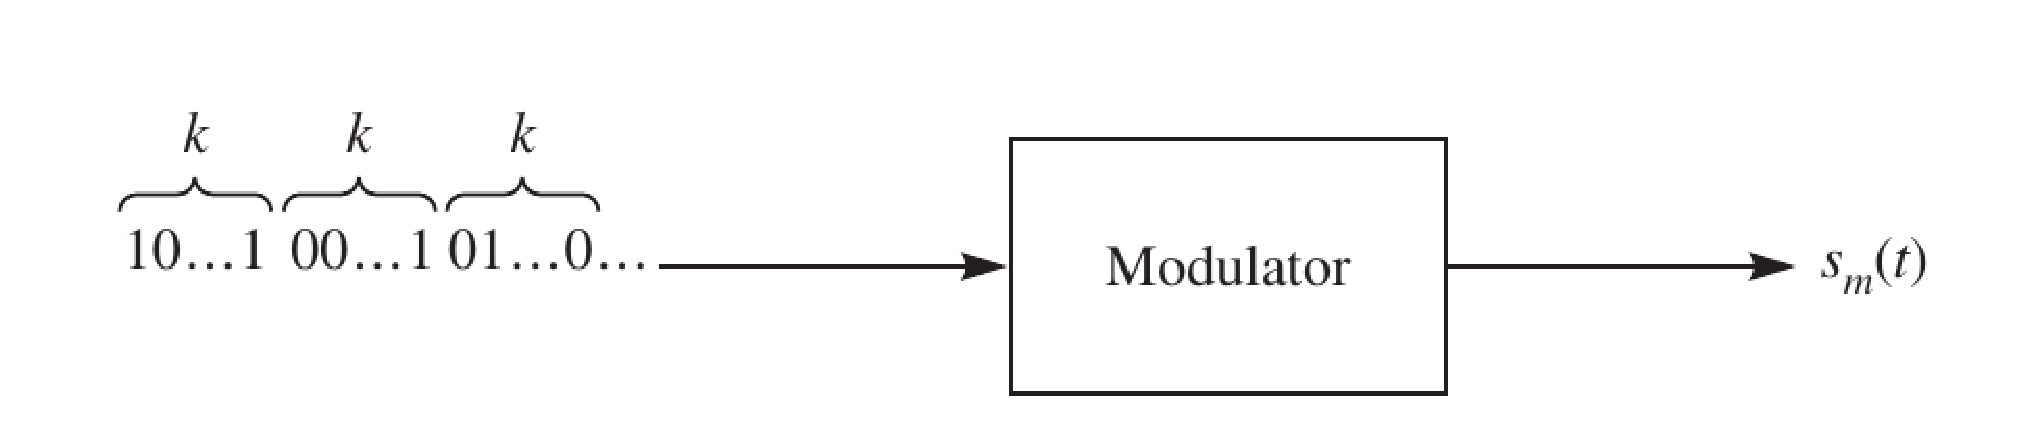
\includegraphics[width=0.7\columnwidth]{figs/mapping}
	  \end{center}
	\end{figure}

\end{frame}

\begin{frame}
	\frametitle{Modulação por amplitude de pulso (PAM)}

	
	   \begin{itemize}
	    \item Amplitude diferencia as formas de onda.
	    \item Formas de onda podem ser representadas como:
	    \begin{align*}
		  s_m(t) &= \re[A_m g(t) e^{j2\pi f_c t}] \\
		  &= A_m g(t) \cos 2\pi f_c t , \quad m=1,2,\ldots, M, \quad 0 \leq t \leq T
	    \end{align*}
	    \item Onde $\{A_m, 1 \leq m \leq M \}$ denota o conjunto de $M=2^k$ possíveis amplitudes, associadas aos blocos de $k$ bits ou \textit{símbolos}.
	    \item Possíveis valores de $A_m$:
	    \begin{equation*}
		A_m = (2m-1-M)d, \quad m=1,2,\ldots,M
	    \end{equation*}
	      \item Onde $2d$ é a distância entre amplitudes de sinais adjacentes.
	      \item O pulso de sinal $g(t)$ é real e sua forma afeta o espectro do sinal transmitido
	   \end{itemize}
	

\end{frame}

\begin{frame}
	\frametitle{Modulação por amplitude de pulso (PAM)}

	\begin{itemize}
	  \item Taxa de símbolos: $R/k$
	  \item Intervalo de bit: $T_b = 1/R$
	  \item Intervalo de símbolo: $T = k/R = kT_b$
	  \item Energia de sinal PAM:
	  \begin{equation*}
	      \mathcal{E}_m = \int_0^T s_m^2(t) dt = \frac{1}{2}A_m^2\int_0^T g^2(t) dt = \frac{1}{2}A_m^2 \mathcal{E}_g
	  \end{equation*}
	   \item Sinais PAM são unidimensionais ($N=1$) e possuem forma geral:
	  \begin{equation*}
	      s_m(t) = s_m f(t)
	  \end{equation*}
	  \item Onde
	      \begin{align*}
		  f(t) &= \sqrt{\frac{2}{\mathcal{E}_g}} g(t) \cos 2\pi f_c t \\
		  s_m &= A_m \sqrt{\energy_g / 2}
	      \end{align*}

	\end{itemize}

\end{frame}

\begin{frame}
	\frametitle{Modulação por amplitude de pulso (PAM)}

	\begin{itemize}
		\item Diagrama de espaço de sinais para sinais digitais PAM.
	\end{itemize}
	
	\begin{figure}[t]
	  \begin{center}
	    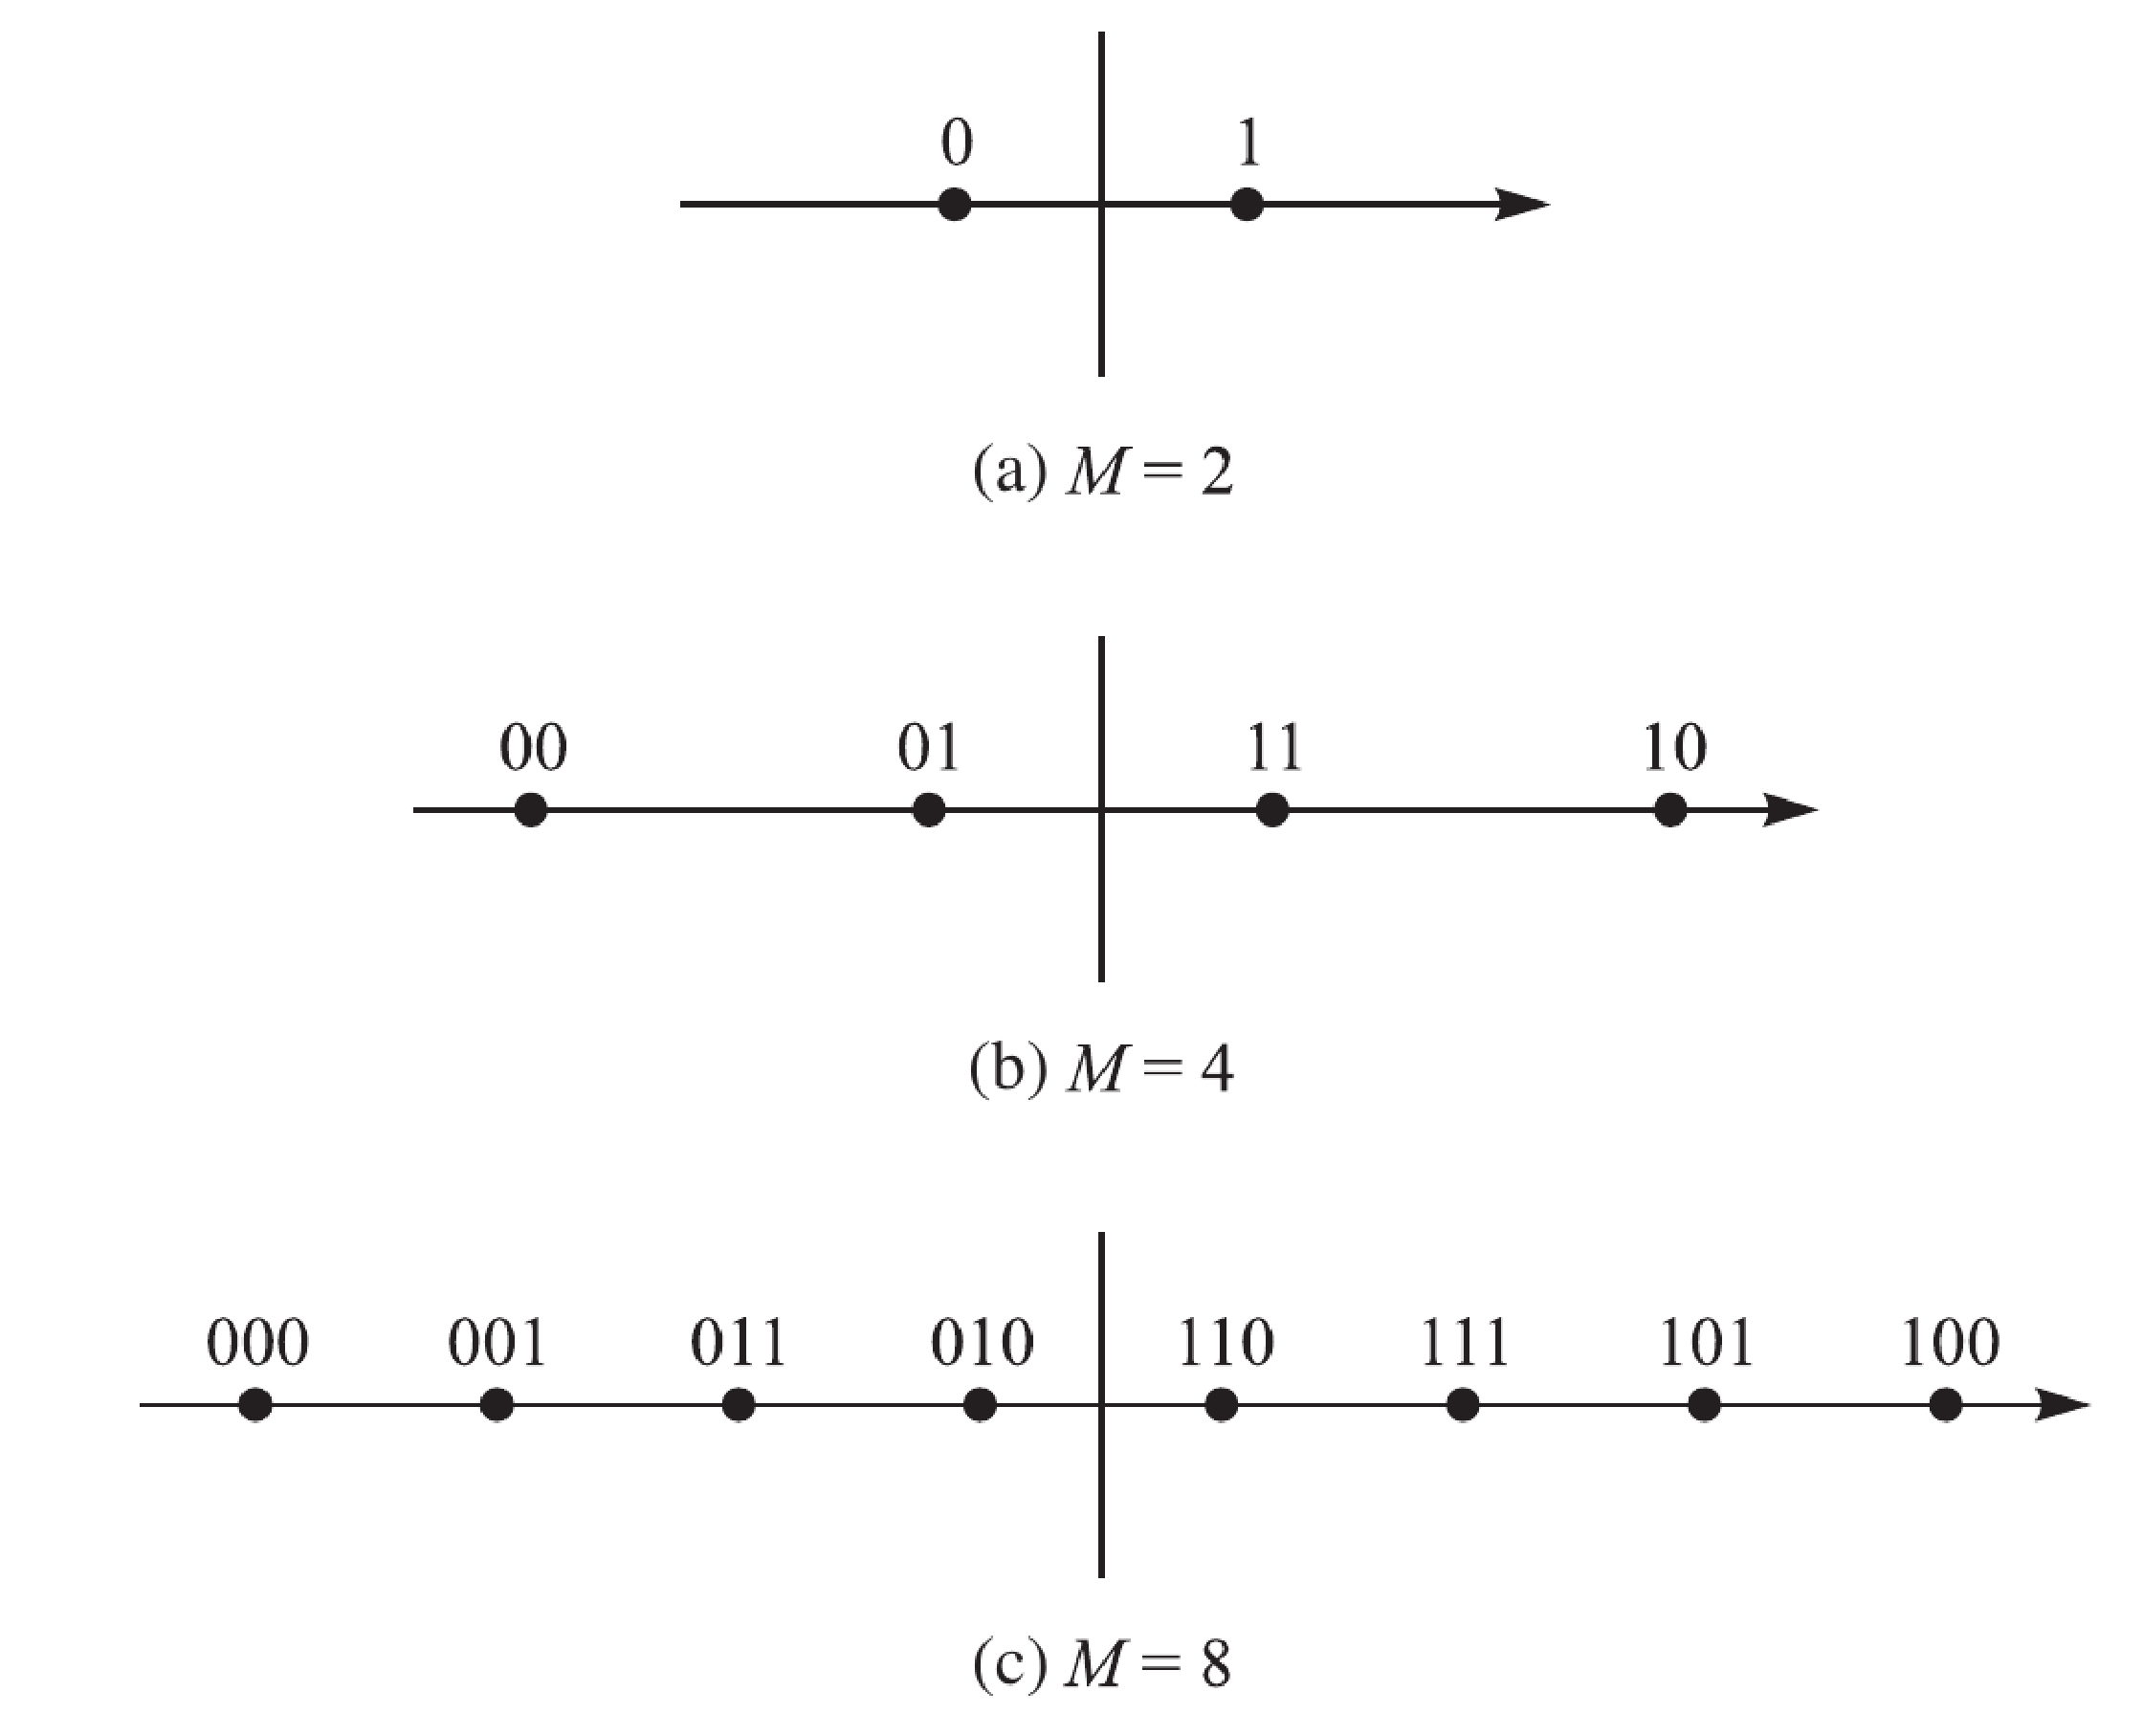
\includegraphics[width=0.6\columnwidth]{figs/4-3-1}
	  \end{center}
	\end{figure}

\end{frame}

\begin{frame}
	\frametitle{Modulação por amplitude de pulso (PAM)}

	\begin{itemize}
		\item PAM também é conhecido como Chaveamento por deslocamento de amplitude (ASK - Amplitude Shift Keying).
		\item Mapeamento dos grupos de bits (símbolos) em amplitudes de sinal:
		\begin{itemize}
			\item Pode ser feito de diversas maneiras.
			\item Mapeamento mais comum: codificação Gray, na qual sinais de amplitudes adjacentes diferem de 1 dígito binário.
			\item Motivação: erros mais prováveis causados por ruído ocorrem quando amplitudes adjacentes são incorretamente selecionadas.
			\item Na codificação Gray esse tipo de erro leva a somente 1 erro de bit na sequência de $k$ bits.
		\end{itemize}
		\item Caso particular em que $M=2$:
		\begin{itemize}
			\item Propriedade: $s_1(t) = s_2(t)$.
			\item Possuem mesma energia e coeficiente de correlação cruzada igual a -1.
			\item Sinais antipodais. 
		\end{itemize}

	\end{itemize}

\end{frame}

\begin{frame}
	\frametitle{Modulação por amplitude de pulso (PAM)}

	\begin{itemize}
		\item Distância Euclidiana entre qualquer par de pontos de sinal:
		\begin{equation*}
			d_{mn}^{(e)} = \sqrt{(s_m-s_n)^2} = \sqrt{\mathcal{E}_g/2}\, \Bigl|A_m - A_n\Bigr| = d\sqrt{2\mathcal{E}_g}\, \Bigl|m-n\Bigr|
		\end{equation*}
		\item A distância entre um par de pontos adjacentes (distância mínima) é:
		\begin{equation*}
			d_{\text{min}}^{(e)} = d\sqrt{2\mathcal{E}_g}
		\end{equation*}
		\item Sinal PAM $s_m(t)$,  para $m=1, \ldots, M$,  pode ser implementado de forma Double Side Band (DSB) ou Single Side Band (SSB):
		\begin{align*}
			s_{m, \text{DSB}}(t) &= \re\{A_m g(t) e^{j2\pi f_c t}\} \\
			s_{m, \text{SSB}}(t) &= \re\{A_m [g(t) \pm j\hat{g}(t) ] e^{j2\pi f_c t}\}
		\end{align*}
		\item Onde $\hat{g}(t)$ é a transformada de Hilbert de $g(t)$.
		\item PAM também pode ser implementado em canal sem modulação de portadora,  ou seja,  em banda base:
		\begin{equation*}
			s_m(t) = A_m g(t)
		\end{equation*}

	\end{itemize}

\end{frame}

\begin{frame}
	\frametitle{Modulação por amplitude de pulso (PAM)}

	\begin{itemize}
	 \item Sinais PAM em banda base e em banda passante:
	\end{itemize}

	
	\begin{figure}[t]
	  \begin{center}
	    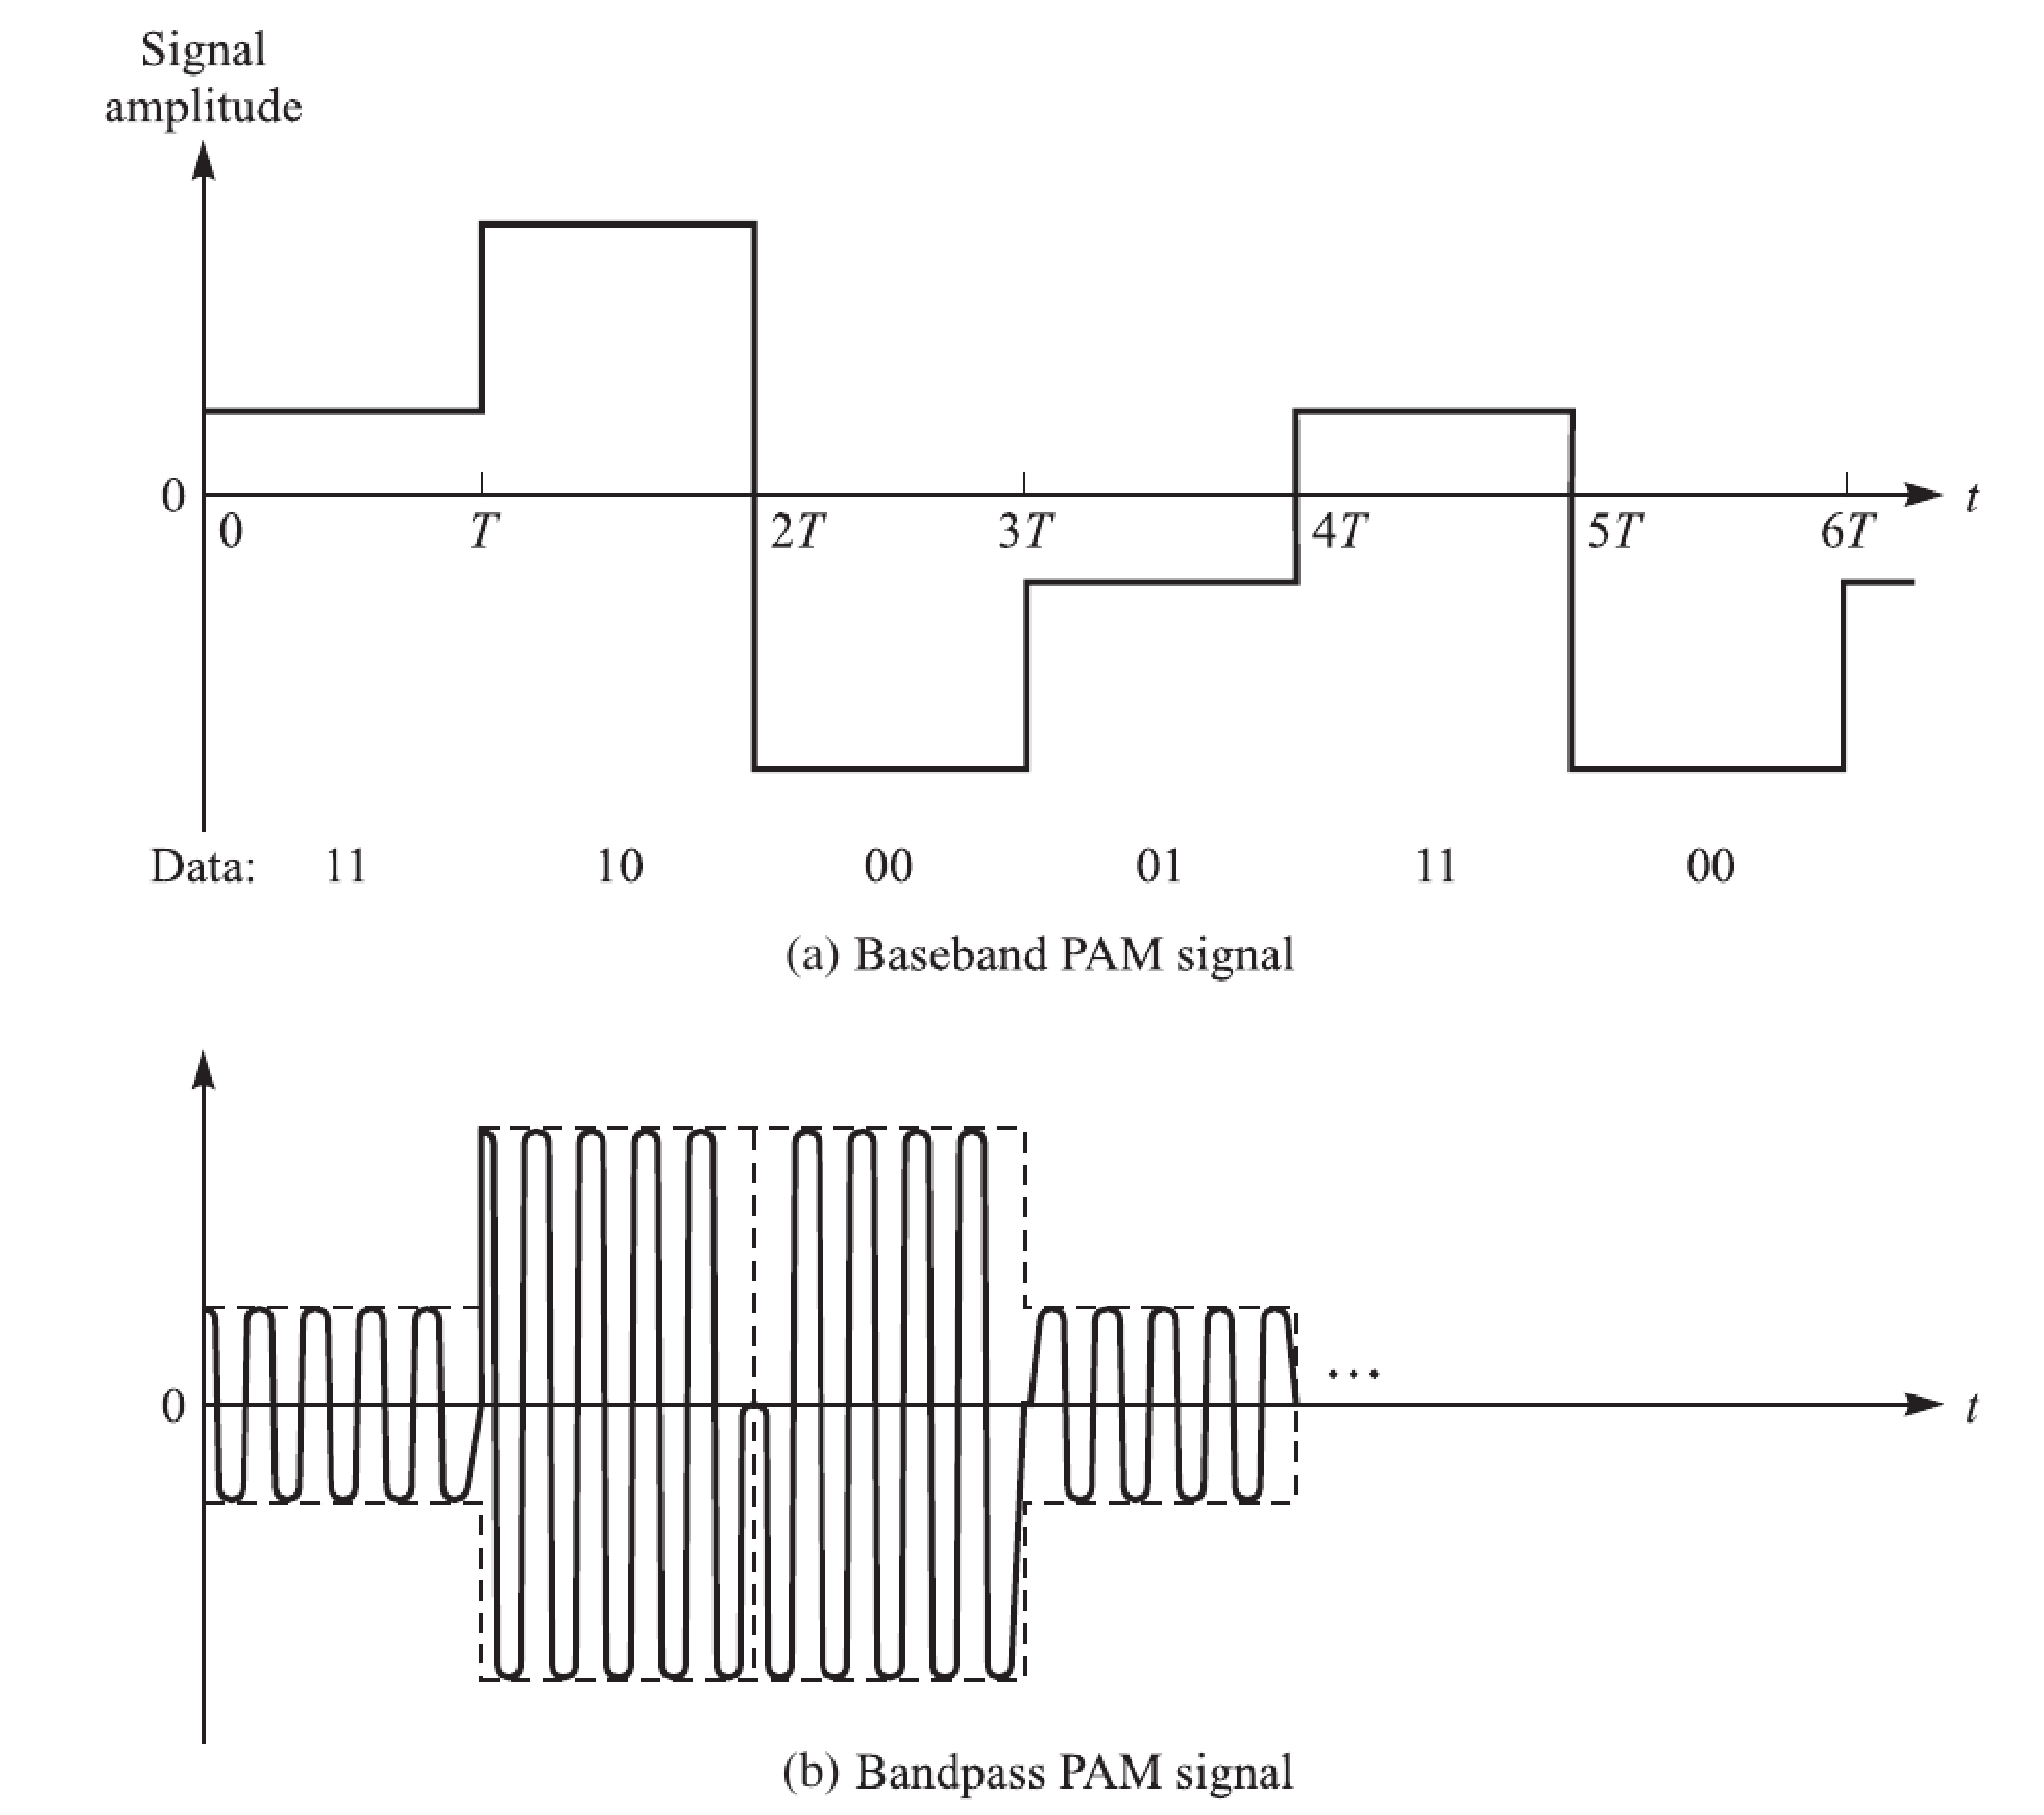
\includegraphics[width=0.6\columnwidth]{figs/4-3-2}
	  \end{center}
	\end{figure}

\end{frame}





% \part{Modulação por amplitude de pulso - PAM}
% \lecture{Modulação por amplitude de pulso - PAM}{lec_pam}

\begin{frame}
	\begin{block}{\centering\large\bfseries Parte 3}
		\centering\large\insertpart
	\end{block}
\end{frame}


\section{PAM em banda base}

\begin{frame}
	\frametitle{PAM em banda base}

	\begin{itemize}
	    \item A escolha da modulação depende das características do meio.
	    \item Os canais podem ser classificados como: banda base (\textit{baseband}) ou banda passante (\textit{bandpass}).	\vspace{-0.3cm}  
	\end{itemize}	
	\begin{figure}[t]	
	  \begin{center}
	    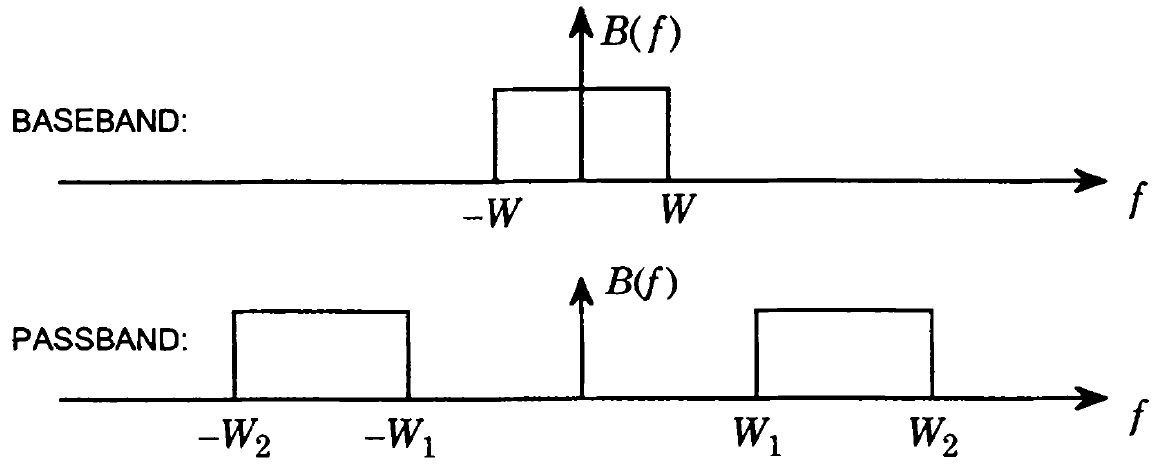
\includegraphics[width=0.5\columnwidth]{figs/pam_01}
	  \end{center}
	\end{figure}
	\vspace{-0.3cm}
	\begin{itemize}
	    \item Sinal PAM em banda base:\vspace{-0.3cm}
	\end{itemize}
	\begin{columns}
		\begin{column}{0.5\textwidth}
		    \begin{equation*}
			s(t) = \sum\limits_{m=-\infty}^{\infty} a_k g(t-kT)
		    \end{equation*}
		\end{column}
		\begin{column}{0.5\textwidth}
		    \begin{itemize}
			\item Taxa de símbolo: $1/T$
			\item Pulso de transmissão: $g(t)$
			\item Símbolos: $\{a_k\}$
		    \end{itemize}
		\end{column}
	\end{columns}	
\end{frame}

\begin{frame}
	\frametitle{PAM em banda base}

	\begin{figure}[t]	
	  \begin{center}
	    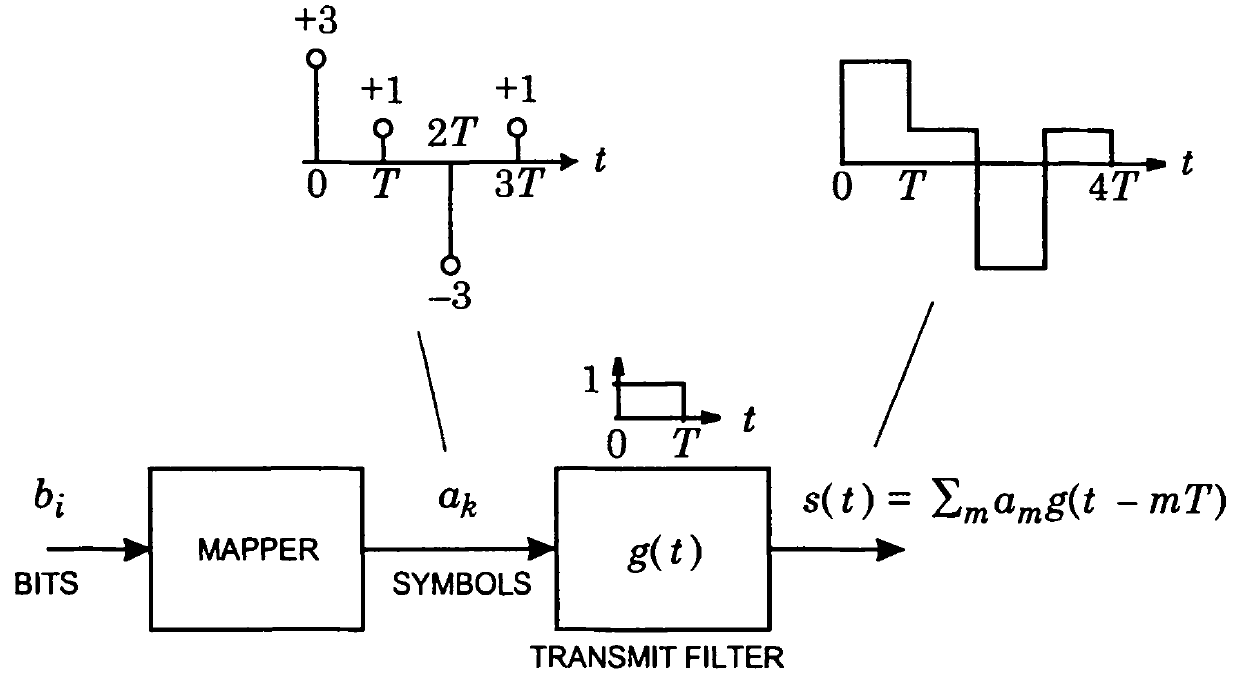
\includegraphics[width=0.5\columnwidth]{figs/pam_02}
	  \end{center}
	\end{figure}	
	\begin{itemize}
	    \item O sinal PAM pode ser interpretado como uma sequência de pulsos superpostos com a amplitude do $k$-ésimo pulso determinada pelo $k$-ésimo símbolo.
	    \item Sequência de bits de entrada é mapeada em uma sequência de símbolos $\{a_k\}$ por um \textit{mapeador}.
	    \item Os símbolos são restritos a um alfabeto finito $\mathcal{A}$, de forma que $a_k \in \mathcal{A}$ e $|\mathcal{A}| = 2^b$, para um inteiro $b$.
	\end{itemize}			
\end{frame}

\begin{frame}
	\frametitle{PAM em banda base}

	\begin{figure}[t]	
	  \begin{center}
	    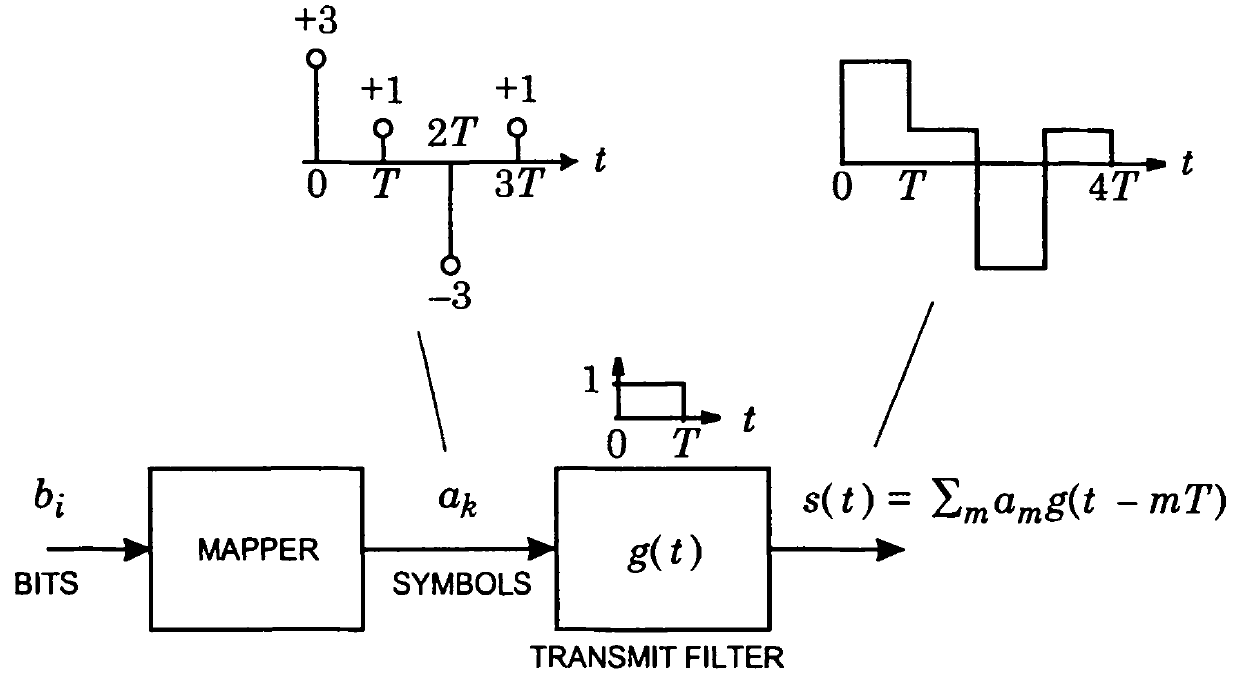
\includegraphics[width=0.5\columnwidth]{figs/pam_02}
	  \end{center}
	\end{figure}	
	\begin{itemize}
	    \item A taxa de símbolos $1/T$ também é chamada de \textit{baud rate}.
	    \item O mapeamento pode ser precedido por uma etapa de codificação de canal, na qual é adicionada redundância à sequência de bits, de forma a reduzir os erros.
	    \item Nesta disciplina vamos assumir que os símbolos que resultam do mapeamento são \textit{iid} (independentes e identicamente distribuídos).
	\end{itemize}			
\end{frame}

\begin{frame}
	\frametitle{Formatação de pulso}

	\begin{itemize}
	    \item Vamos considerar nessa seção o caso sem ruído, tendo como objetivo determinar a relação entre a largura de banda e a taxa de símbolos.
	    \item Considere a amostragem de $s(t)$ em múltiplos inteiros do tempo de símbolo:
	    \begin{align*}
		s(kT) &= \sum\limits_{m=-\infty}^{\infty} a_m g(kT-mT) = a_k * g(kT) \\
		&= \underbrace{a_k g(0)}_{\text{\textcolor{blue}{Termo desejado}}} + \underbrace{\sum\limits_{m\neq k} a_m g(kT-mT)}_{\text{\textcolor{red}{Interferência Inter-simbólica (ISI)}}}
	    \end{align*}
	    \item Condição para que a ISI seja anulada:
	    \begin{equation*}
		    g(kT) = \delta_k
	    \end{equation*}
	\end{itemize}			
\end{frame}

\begin{frame}
	\frametitle{Formatação de pulso}

	\begin{itemize}
	    \item Aplicando a transformada de Fourier obtemos:
	    \begin{equation*}
		    g(kT) = \delta_k \quad \xrightarrow{\mathcal{F}} \quad \frac{1}{T}\sum\limits_{m=-\infty}^{\infty} G\left(f-\frac{m}{T} \right) = 1
	    \end{equation*}
	    \item Obtemos portanto o \textcolor{blue}{\textit{critério de Nyquist}}.
	    \item Um pulso que satisfaz esse critério é chamado de \textit{pulso de Nyquist}.
	    \item Este critério implica que existe uma banda mínima a ser respeitada para se transmitir a uma certa taxa sem ISI.
	\end{itemize}			
	\begin{figure}[t]	
	  \begin{center}
	    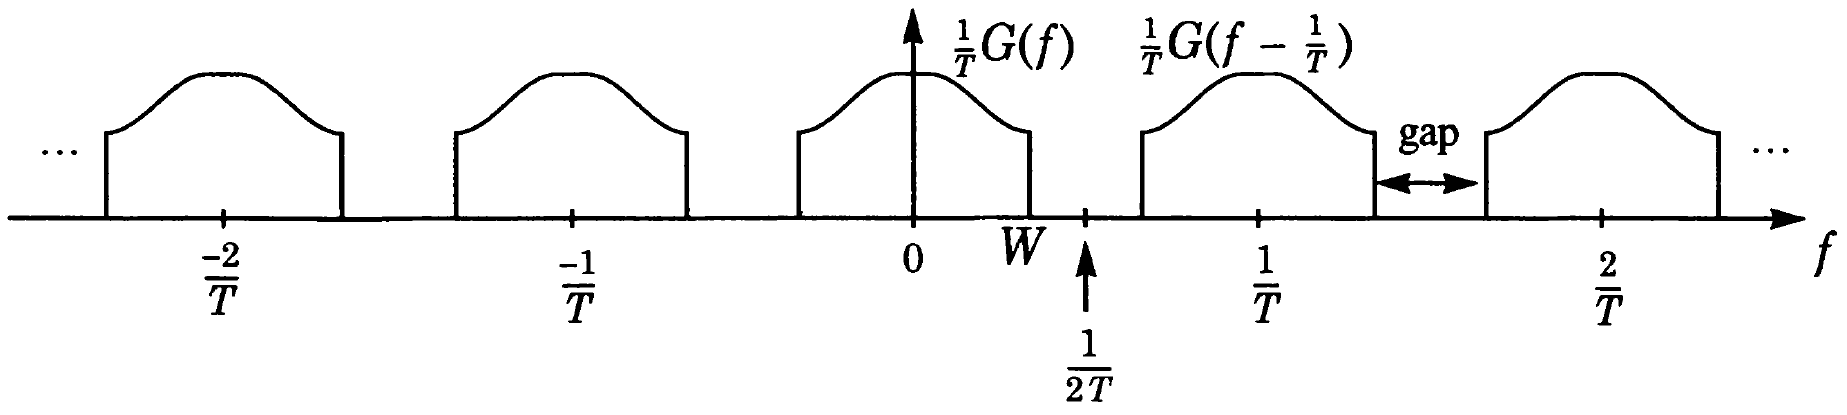
\includegraphics[width=\columnwidth]{figs/pam_03}
	  \end{center}
	\end{figure}
\end{frame}

\begin{frame}
	\frametitle{Formatação de pulso}

	\begin{itemize}
	    \item Largura de banda mínima para evitar ISI: $W \geq 1/(2T)$
	    \item Máxima taxa de símbolos correspondente: $1/T \leq 2W$
	    \item Mas não é qualquer pulso que satisfaz o critério de Nyquist: o espectro resultante deve ser uma constante.
	    \item Exemplo de pulso que satisfaz o critério:
	\end{itemize}			
	\begin{figure}[t]	
	  \begin{center}
	    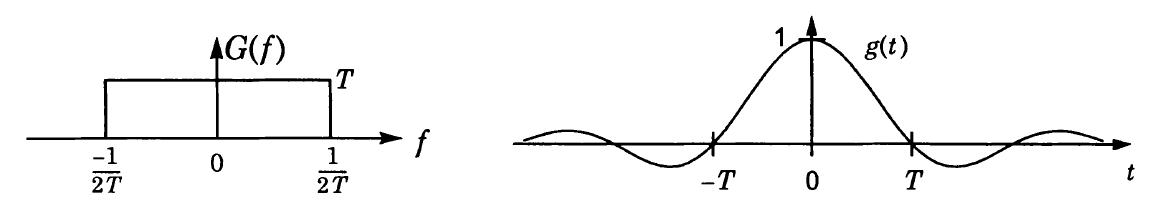
\includegraphics[width=\columnwidth]{figs/pam_04}
	  \end{center}
	\end{figure}
	\small
	$G(f) = \begin{cases}
		    T , \quad -1/(2T) \leq f \leq 1/(2T) \\
		    0, \quad \text{c.c.}
		\end{cases}  \xrightarrow{\mathcal{F}^{-1}} \quad g(t) = \frac{\sin(\pi t/T)}{\pi t/T}$

\end{frame}


\begin{frame}
	\frametitle{Formatação de pulso}

	\begin{itemize}
	    \item Ilustração de uso do pulso de Nyquist.
	    \item Considere símbolos sucessivos com valores $a_0=1$ e $a_1=2$.
	    \item Contribuição dos símbolos ao sinal:
	\end{itemize}			
	\begin{figure}[t]	
	  \begin{center}
	    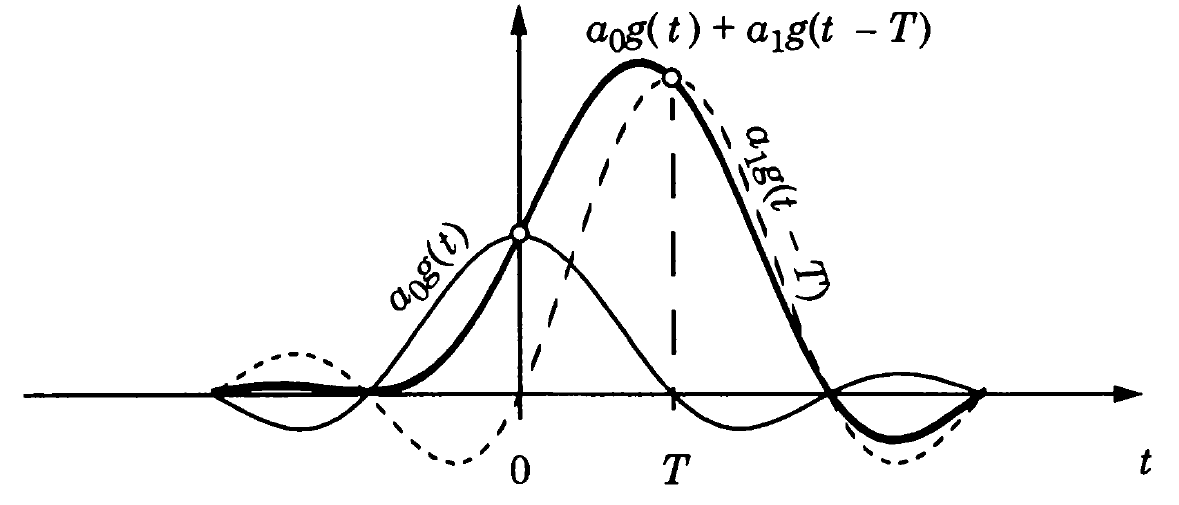
\includegraphics[width=0.7\columnwidth]{figs/pam_05}
	  \end{center}
	\end{figure}
\end{frame}


\begin{frame}
	\frametitle{Formatação de pulso}

	\begin{itemize}
	    \item O pulso ideal retangular (na frequência) possui a propriedade desejável de mínima banda, mas apresenta problemas de realização prática.
	    \item Um pulso prático deve apresentar um fator de excesso de banda $\alpha$, de forma que:
	    \begin{equation*}
		W = \frac{1+\alpha}{2T}
	    \end{equation*}
	    \item Pulso ideal ocorre para $\alpha=0$;
	    \item Valores práticos de excesso de banda: 10\% a 100\%.
	    \item Custo-benefício entre aumento de banda e simplicidade de implementação.
	    \item $\alpha$ também é chamado de fator de \textit{roll-off}.
	    \item Existem múltiplas soluções de pulsos que satisfazem o critério de Nyquist para $\alpha >0$.
	\end{itemize}			
\end{frame}

\begin{frame}
	\frametitle{Formatação de pulso}

	\begin{itemize}
	    \item Pulso cosseno levantado
	\end{itemize}
	\begin{small}
	\begin{align*}
	    g(t) &= \left( \frac{\sin(\pi t/T)}{\pi t/T} \right) \left( \frac{\cos(\alpha \pi t/T)}{1-(2\alpha t/T)^2} \right) \\
	    G(f) &= \begin{cases}
			T, & |f| \leq \frac{1-\alpha}{2T} \\
			T\cos^2\left[ \frac{\pi T}{2\alpha} \left(|f| - \frac{1-\alpha}{2T} \right) \right], & \frac{1-\alpha}{2T} < |f| \leq \frac{1+\alpha}{2T} \\
			0, & \frac{1+\alpha}{2T} < |f|
	            \end{cases}
	\end{align*}
	\end{small}
	\begin{figure}[t]	
	  \begin{center}
	    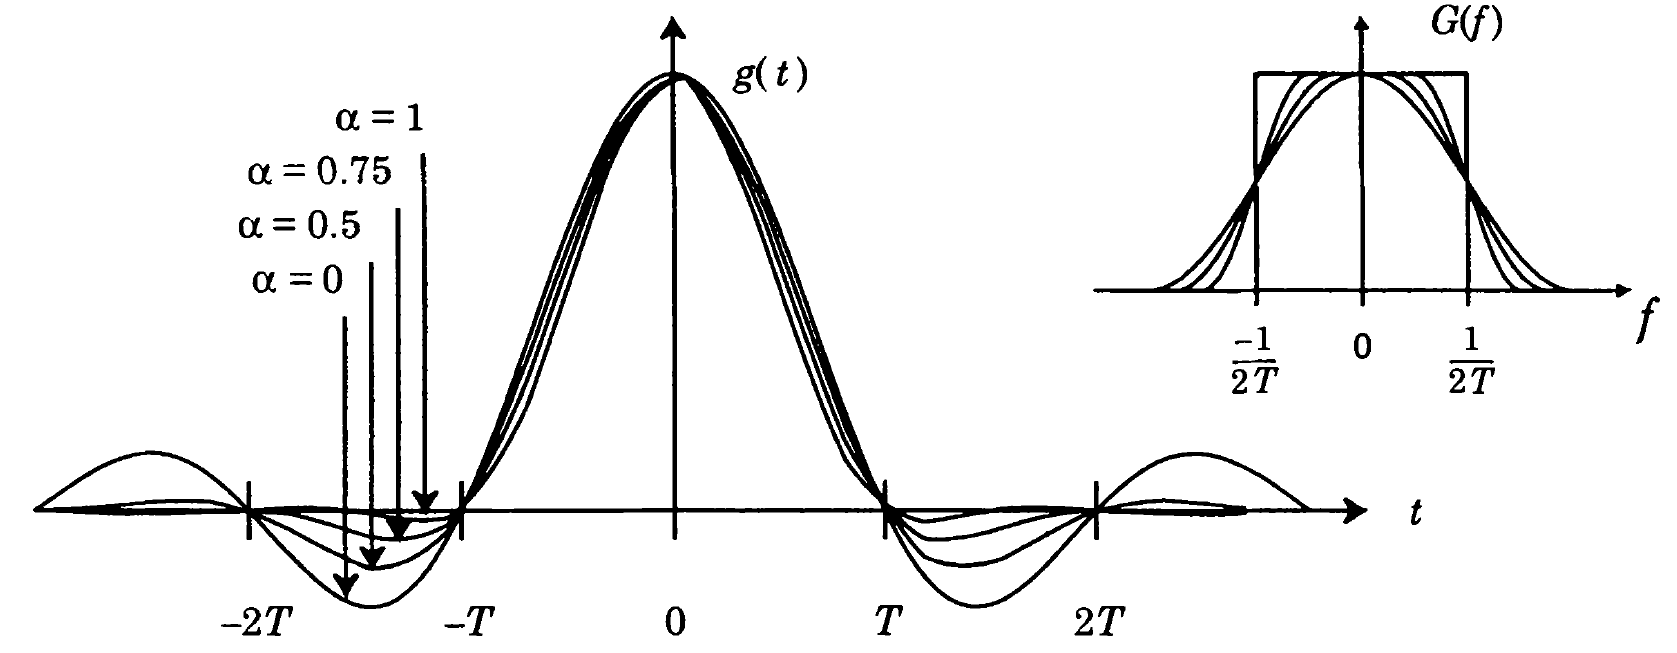
\includegraphics[width=0.8\columnwidth]{figs/pam_06}
	  \end{center}
	\end{figure}
\end{frame}

\begin{frame}
	\frametitle{Formatação de pulso}

	\begin{itemize}
	    \item Existe um número infinito de pulsos que satisfazem o critério de Nyquist.
	    \item Seguem alguns exemplos adicionais:
	\end{itemize}	
	\begin{figure}[t]	
	  \begin{center}
	    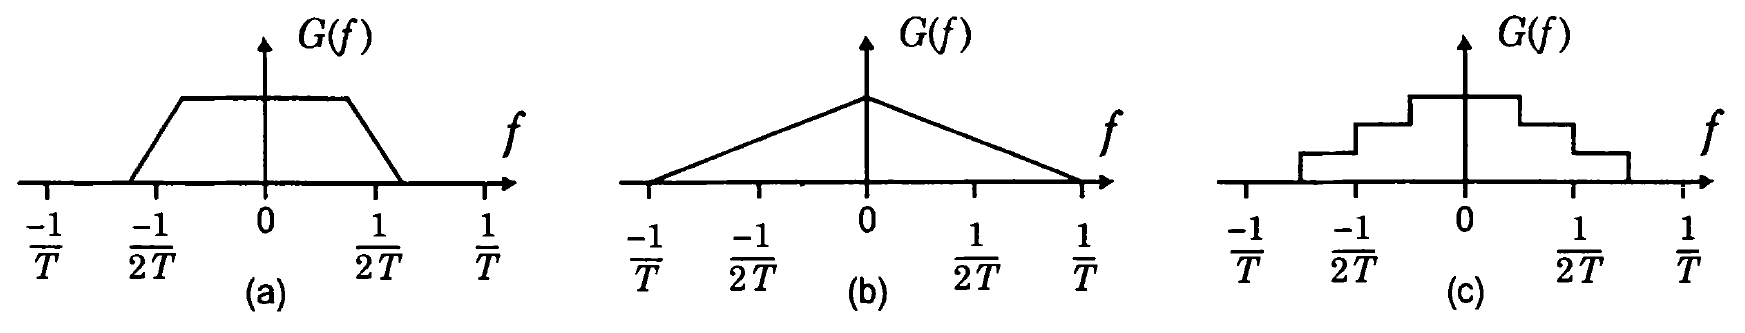
\includegraphics[width=0.8\columnwidth]{figs/pam_07}
	  \end{center}
	\end{figure}
\end{frame}

\begin{frame}
	\frametitle{Impacto da filtragem sobre o PAM}

	\begin{itemize}
	    \item Consideremos agora o impacto do canal, modelado como um filtro linear invariante no tempo com resposta ao impulso $b(t)$ e ruído aditivo $n(t)$.
	\end{itemize}	
	\begin{figure}[t]	
	  \begin{center}
	    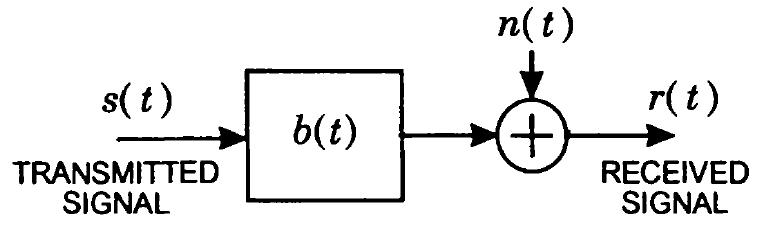
\includegraphics[width=0.4\columnwidth]{figs/pam_08}
	  \end{center}
	\end{figure}
	\begin{itemize}
	    \item Aplicando o sinal PAM nesse modelo obtemos:
	    \begin{align*}
		r(t) = \int_{-\infty}^{\infty}b(\tau)\sum\limits_{m=-\infty}^{\infty} a_m g(t-mT-\tau)d\tau + n(t)
	    \end{align*}
	    \item Para $h(t) = b(t)*g(t)$, chamado de pulso recebido, obtemos
	    \begin{equation*}
		r(t) = \sum\limits_{m=-\infty}^{\infty} a_m h(t-mT) + n(t)
	    \end{equation*}
	\end{itemize}	
\end{frame}

\begin{frame}
	\frametitle{Impacto da filtragem sobre o PAM}

	\begin{itemize}
	    \item Se o sinal transmitido é PAM, o sinal recebido também é PAM, mas com um diferente formato de pulso e com a adição de ruído.
	    \item Filtro de recepção:
	    \begin{itemize}
		\item Compensação da distorção do canal.
		\item Diminuição do efeito do ruído aditivo.
		\item Condicionamento do sinal recebido antes da amostragem.
		\item Pode ser projetado para evitar ISI após amostragem.
	    \end{itemize}
	\end{itemize}		
	\begin{figure}[t]	
	  \begin{center}
	    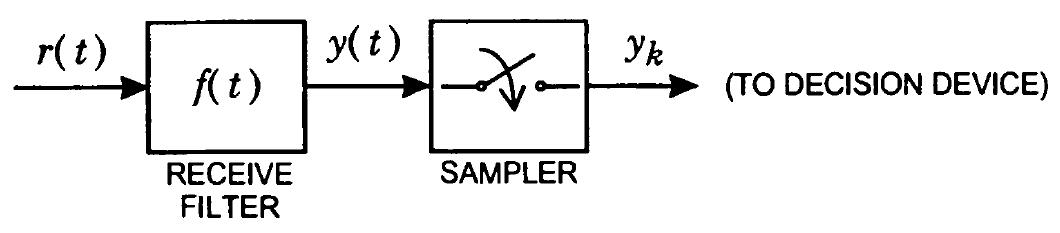
\includegraphics[width=0.6\columnwidth]{figs/pam_09}
	  \end{center}
	\end{figure}
\end{frame}

\begin{frame}
	\frametitle{Impacto da filtragem sobre o PAM}

	\begin{itemize}
	    \item Saída do filtro de recepção antes da amostragem:
	    \begin{equation*}
		y(t) = \sum\limits_{\infty}^{\infty} a_m p(t-mT) + n'(t)
	    \end{equation*}
	    \item Onde $p(t)$ é o formato de pulso resultante, dado por:
	    \begin{equation*}
		p(t) = g(t) * b(t) * f(t) \quad \xrightarrow{\mathcal{F}} \quad P(f) = G(f)B(f)F(f)
	    \end{equation*}
	    \item Para evitar ISI, o pulso resultante deve ser Nyquist, e não somente $g(t)$, portanto:
	    \begin{equation*}
		    p(kt) = \delta_k \quad \xrightarrow{\mathcal{F}} \quad \sum\limits_{m=-\infty}^{\infty} P\left(f-\frac{m}{T} \right) = T
	    \end{equation*}
	\end{itemize}		
\end{frame}

\begin{frame}
	\frametitle{ISI e Diagramas de olho}

	\begin{itemize}
	    \item Cancelamento perfeito da ISI é difícil de ser alcançado:
	    \begin{itemize}
		\item Imperfeições na estimativa de canal.
		\item Limitações práticas de implementação do pulso de transmissão.
	    \end{itemize}
	    \item Diagrama de olho:
	    \begin{itemize}
		\item Ilustra a degradação do sinal.
		\item Pode ser gerado em osciloscópio.
		\item Ferramenta de auxílio na etapa de projeto do sistema.
		\item Consiste da superposição de várias pequenas partes de um sinal.
	    \end{itemize}
	    \item A presença de ISI tende a fechar o olho verticalmente.
	    \item Instante ideal de amostragem é o ponto de máxima abertura.
	    \item Abertura horizontal é importante para reduzir o impacto de erros de temporização.
	\end{itemize}		
\end{frame}

\begin{frame}
	\frametitle{ISI e Diagramas de olho}

	\begin{itemize}
	 \item PAM binário com 50\% de banda excedente.
	\end{itemize}	
	\begin{figure}[t]	
	  \begin{center}
	    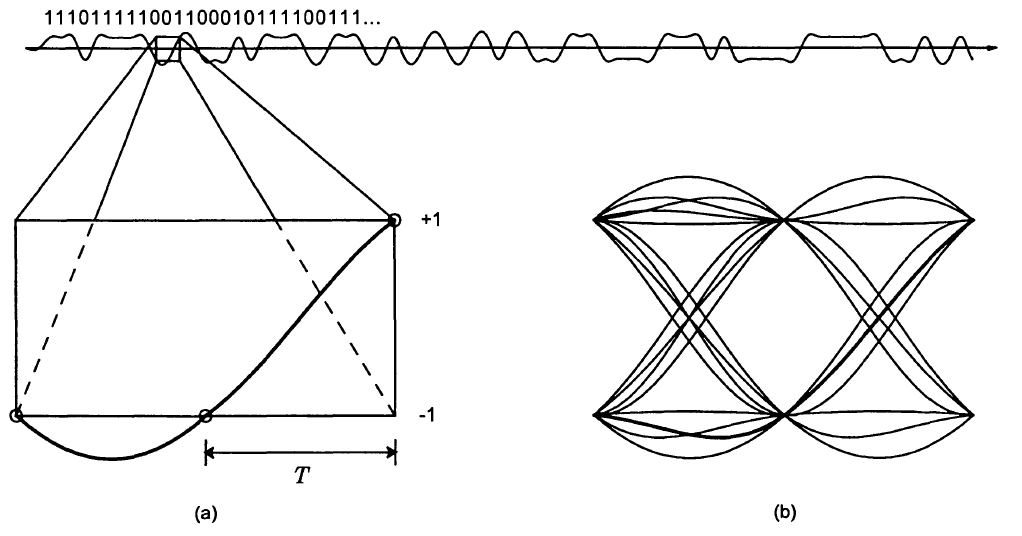
\includegraphics[width=0.9\columnwidth]{figs/pam_10}
	  \end{center}
	\end{figure}
\end{frame}

\begin{frame}
	\frametitle{ISI e Diagramas de olho}

	\begin{columns}	
	    \begin{column}{0.5\textwidth}
		\begin{figure}[t]	
		    \begin{center}
			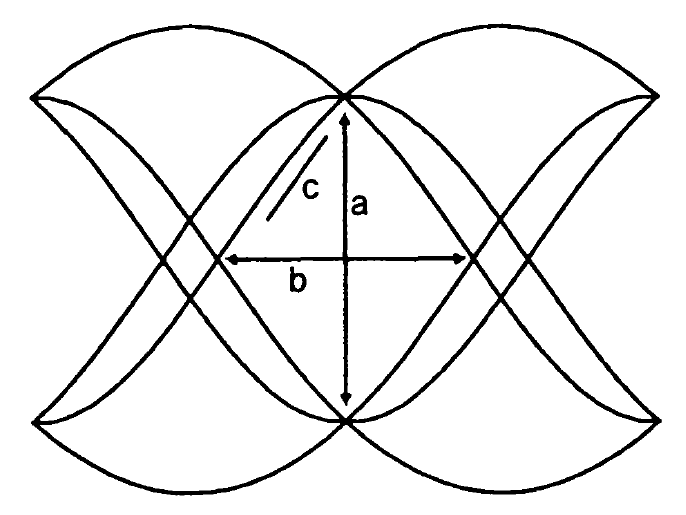
\includegraphics[width=0.8\columnwidth]{figs/pam_11}
		    \end{center}
		\end{figure}
	    \end{column}

	    \begin{column}{0.5\textwidth}
		\begin{enumerate}[a)]
		    \item Abertura vertical indica imunidade a ruído
		    \item Abertura horizontal indica imunidade a erros de temporização.
		    \item Inclinação da pálpebra interna indica a sensibilidade a \textit{jitter} de temporização.
		\end{enumerate}		 
	    \end{column}	
	\end{columns}

\end{frame}

\begin{frame}
	\frametitle{ISI e Diagramas de olho}

	\begin{itemize}
	 \item Diagramas de olho para (a) 25\% e (b) 100\% de banda excedente.
	\end{itemize}	
	
	\begin{figure}[t]	
	  \begin{center}
	    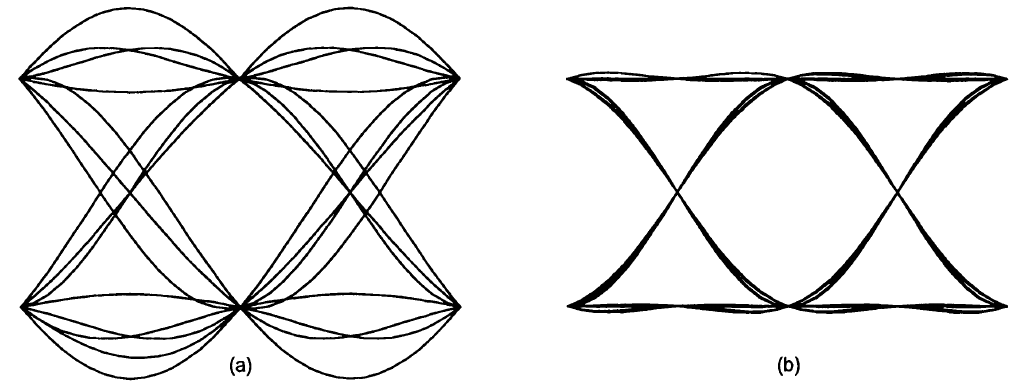
\includegraphics[width=0.9\columnwidth]{figs/pam_12}
	  \end{center}
	\end{figure}
\end{frame}

\begin{frame}
	\frametitle{Taxa de bits e eficiência espectral}

	\begin{itemize}
	  \item Os símbolos são escolhidos, de forma independente e uniforme, do alfabeto $\mathcal{A}$, de tamanho $|\mathcal{A}|$.
	  \item Cada símbolo carrega $\log_2 |\mathcal{A}|$ bits de informação.
	  \item Taxa de bits do PAM:
	  \begin{equation*}
	    R_b = \frac{\log_2 |\mathcal{A}|}{T} \quad \text{ bit/s}
	  \end{equation*}
	  \item Formas de aumentar a taxa:
	  \begin{itemize}
	    \item Aumentar a ordem da modulação (limitação de potência e impacto do ruído)
	    \item Aumentar a taxa de símbolos $1/T$ (limitação de banda e impacto da ISI)
	  \end{itemize}
	  \item Eficiência espectral:
	  \begin{equation*}
	      \nu = \frac{\text{taxa de bits}}{\text{banda}} = \frac{R_b}{W} \quad \text{bit/s/Hz}
	  \end{equation*}
	\end{itemize}	
\end{frame}

\begin{frame}
	\frametitle{Taxa de bits e eficiência espectral}

	\begin{itemize}
	  \item Para o PAM temos: $W=(1+\alpha)/(2T)$
	  \item A eficiência espectral pode ser simplificada para:
	  \begin{equation*}
	      \nu = \frac{R_b}{W} = \frac{\log_2 |\mathcal{A}| / T}{(1+\alpha)/(2T)} = \frac{2\log_2 |\mathcal{A}|}{1+\alpha}
	  \end{equation*}
	  \item Também podemos isolar o tamanho do alfabeto:
	  \begin{equation*}
	      |\mathcal{A}| = 2^{(1+\alpha)\nu / 2}
	  \end{equation*}
	  \item Para o caso do filtro ideal com $\alpha=0$, temos:
	  \begin{equation*}
	      \nu_{\text{max}} = 2 \log_2 |\mathcal{A}| \quad \text{e} \quad |\mathcal{A}| =  2^{\nu_{\text{max}} / 2}
	  \end{equation*}  

	\end{itemize}	
\end{frame}


\section{PAM em banda passante}

\begin{frame}
	\frametitle{Representação em banda passante do PAM}

	\begin{itemize}
	  \item Comunicações práticas normalmente ocorrem em banda passante.
	  \begin{figure}[t]	
	    \begin{center}
	      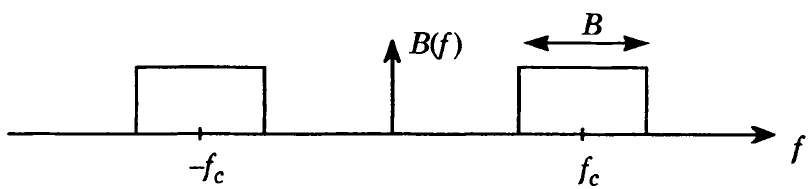
\includegraphics[width=0.6\columnwidth]{figs/pam_13}
	    \end{center}
	  \end{figure}
	  \item Representações em banda passante do PAM:
	  \begin{itemize}
	    \item PAM \textit{double-sideband} (PAM-DSB)
	    \item PAM \textit{single-sideband} (PAM-SSB)
	    \item PAM \textit{em banda passante}
	  \end{itemize}
	\end{itemize}
\end{frame}

\begin{frame}
	\frametitle{PAM-DSB}

	\begin{itemize}
	  \item PAM-DSB modula diretamente o sinal PAM aplicando oscilador local:
	  \begin{equation*}
	      s(t) = \sqrt{2} \cos(2\pi f_c t) \sum_k a_k g(t-kT)
	  \end{equation*}
	  \item Sinal PAM de banda $B/2$ passa a ocupar $B$ em banda passante.
	  \item Aplicando o critério de Nyquist:
	  \begin{equation*}
	      \frac{1}{2T} \leq (B/2) \quad \Longrightarrow \quad \frac{1}{T} \leq B
	  \end{equation*}
	  \item Desta forma a eficiência espectral cai para a metade da eficiência do PAM em banda base:
	  \begin{equation*}
	      \nu_{\text{max}}^{\text{DSB}} = \frac{R_b}{B} = \frac{\log_2 |\mathcal{A}|/T}{1/T} = \log_2 |\mathcal{A}|
	  \end{equation*}
	\end{itemize}
\end{frame}

\begin{frame}
	\frametitle{PAM-SSB}

	\begin{itemize}
	  \item PAM-SSB evita a redundância das faixas laterais, transmitindo somente uma das faixas.
	  \item Pode ser implementado usando um divisor de fase:
	  \begin{figure}[t]	
	    \begin{center}
	      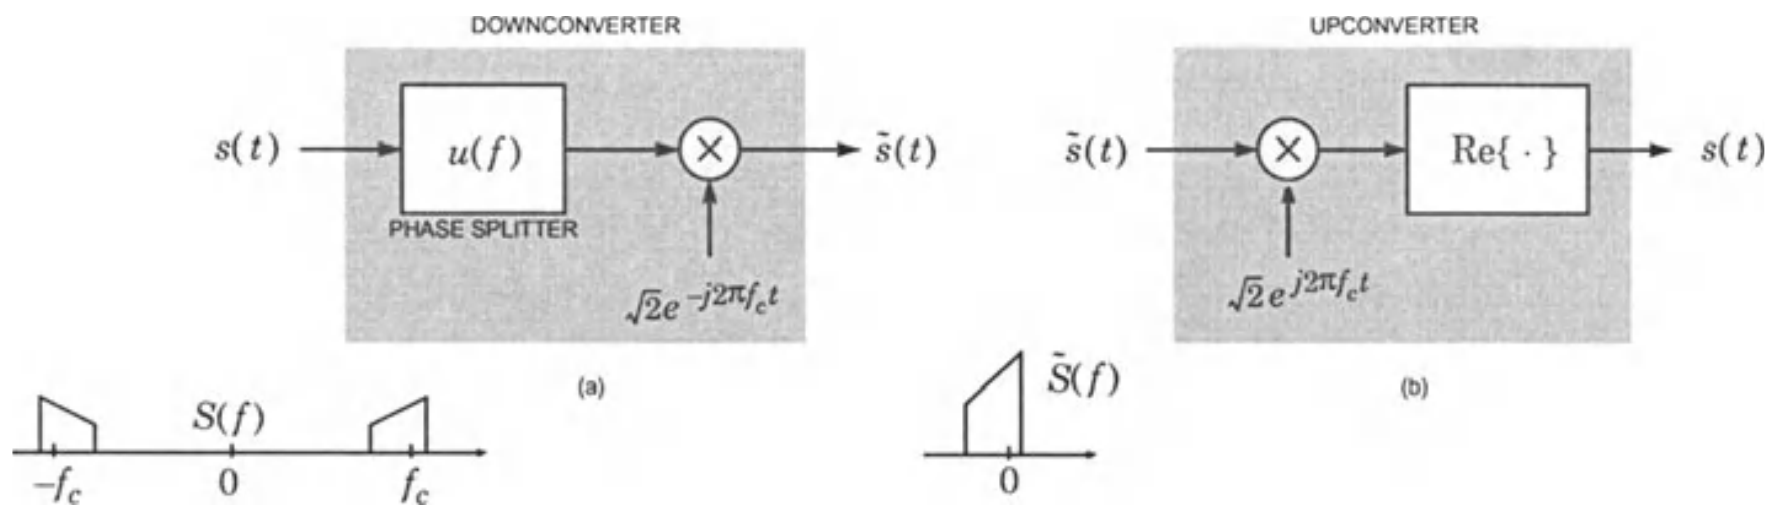
\includegraphics[width=0.9\columnwidth]{figs/pam_22}
	    \end{center}
	  \end{figure}
	  \item Mesma eficiência do PAM em banda base.
	  \item Dificuldade prática de implementação.
	\end{itemize}
	
\end{frame}

\begin{frame}
	\frametitle{PAM em banda passante}

	\begin{itemize}
	  \item Modificação do PAM-DSB para aumentar sua eficiência.
	  \item Definição de componentes em fase $\{ a_k^I \}$ e quadratura $\{ a_k^Q \}$.
	  \begin{equation*}
	      s(t) = \sqrt{2} \cos(2\pi f_c t) \sum_k a_k^I g(t-kT) - \sqrt{2} \sin(2\pi f_c t) \sum_k a_k^Q g(t-kT)
	  \end{equation*}
	  \item O componente em quadratura representa um recurso extra.
	  \item Mesma banda do PAM-DSB, mas com o dobro da eficiência espectral, pois transporta o dobro de informação.
	  \item Classificação com relação à escolha das sequências $\{ a_k^I \}$ e $\{ a_k^Q \}$:
	  \begin{itemize}
	    \item Escolha independente: QAM (modulação em amplitude e quadratura)
	    \item Escolha conjunta: PAM \textit{em banda passante}.
	  \end{itemize}

	\end{itemize}	
\end{frame}

\begin{frame}
	\frametitle{PAM em banda passante}

	\begin{itemize}
	  \item Diagrama de um transmissor PAM em banda passante:
	    \begin{figure}[t]	
	      \begin{center}
		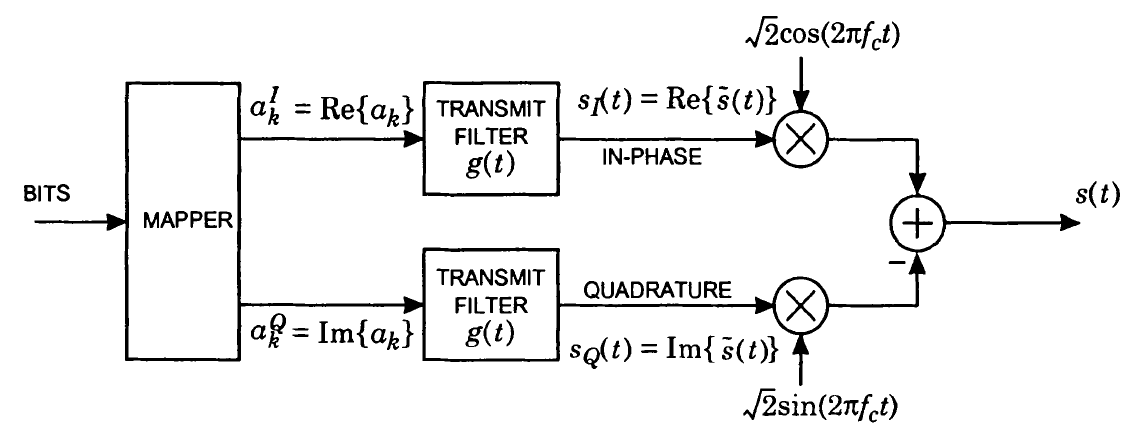
\includegraphics[width=0.9\columnwidth]{figs/pam_14}
	      \end{center}
	    \end{figure}
	\end{itemize}	
\end{frame}

\begin{frame}
	\frametitle{PAM em banda passante}

	\begin{itemize}
	  \item Representação em termos da envoltória complexa:
	  \begin{equation*}
	      s(t) = \sqrt{2} \mathrm{Re}\{ \tilde{s}(t)e^{j2\pi f_c t} \}
	  \end{equation*}
	  \item Onde $\tilde{s}(t)$ corresponde ao equivalente passa-baixa:
	  \begin{equation*}
	      \tilde{s}(t) = \sum_k a_k g(t-kT) \; \text{, com} \quad a_k = a_k^I + j a_k^Q
	  \end{equation*}
	  \item Sinal semelhante ao PAM em banda base, mas com símbolos complexos e pulso real.
	\end{itemize}	
\end{frame}

\begin{frame}
	\frametitle{PAM em banda passante}

	\begin{itemize}
	  \item Implementação alternativa do transmissor PAM baseada na representação complexa:
	    \begin{figure}[t]	
	      \begin{center}
		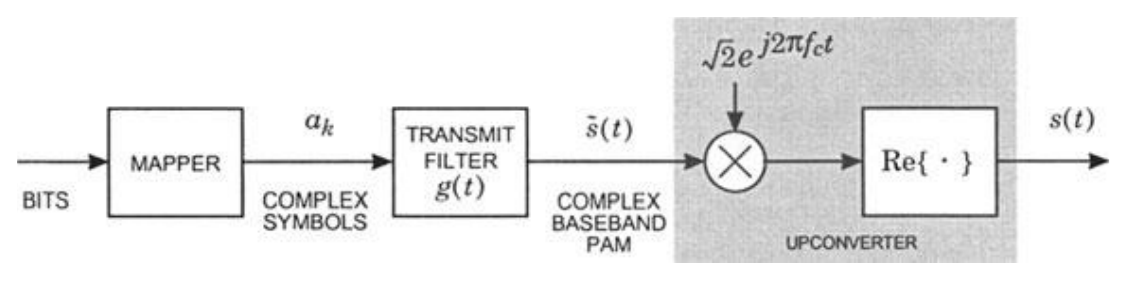
\includegraphics[width=0.75\columnwidth]{figs/pam_15}
	      \end{center}
	    \end{figure}
	   \item Essa implementação é menos eficiente (parte imaginária é computada e descartada), mas a representação complexa é mais compacta e concisa.
	   \item PAM \textit{em banda passante} e SSB duplicam a eficiência do PAM-DSB.
	  \begin{itemize}
	    \item SSB fixa a taxa de bits e corta a banda pela metade.
	    \item PAM \textit{em banda passante} duplica a taxa de bits e mantém a banda.
	  \end{itemize}
	\end{itemize}	
\end{frame}

\begin{frame}
	\frametitle{PAM em banda passante}

	\begin{itemize}
	  \item Representações em: a) fase e quadratura; b) envoltória complexa.
	  \item Terceira representação baseada em coordenadas polares:
	  \begin{align*}
	      a_m &= c_m e^{j \theta_m} \\
	      s(t) &= \sqrt{2} \mathrm{Re} \left\{ \sum_{m=-\infty}^{\infty} c_m e^{j(2\pi f_c t + \theta_m)} g(t-mT) \right\} \\
 	      &= \sqrt{2} \sum_{m=-\infty}^{\infty} c_m \cos(2\pi f_c t + \theta_m) g(t-mT)
	  \end{align*}
	  \item Amplitude e fase da portadora são determinadas por $a_m$.
	  \item Também chamado de AM/PM.
	  \item Indica que o PSK (chaveamento por deslocamento de fase) é um caso particular do PAM em banda passante.
	\end{itemize}	
\end{frame}

\begin{frame}
	\frametitle{Constelações}

	\begin{itemize}
	  \item O alfabeto é o conjunto $\mathcal{A}$ de símbolos disponíveis para transmissão.
	  \item Exemplos:
	  \begin{itemize}
		\item Alfabeto real: $\mathcal{A} = \{ -3. -1, +1, +3 \}$
		\item Alfabeto complexo: $\mathcal{A} = \{ -1. -j, +1, +j \}$
	  \end{itemize}
	    \item Constelação de sinais: conjunto de pontos do alfabeto dispostos em um plano complexo.
	\end{itemize}	
	\begin{figure}[t]	
	      \begin{center}
		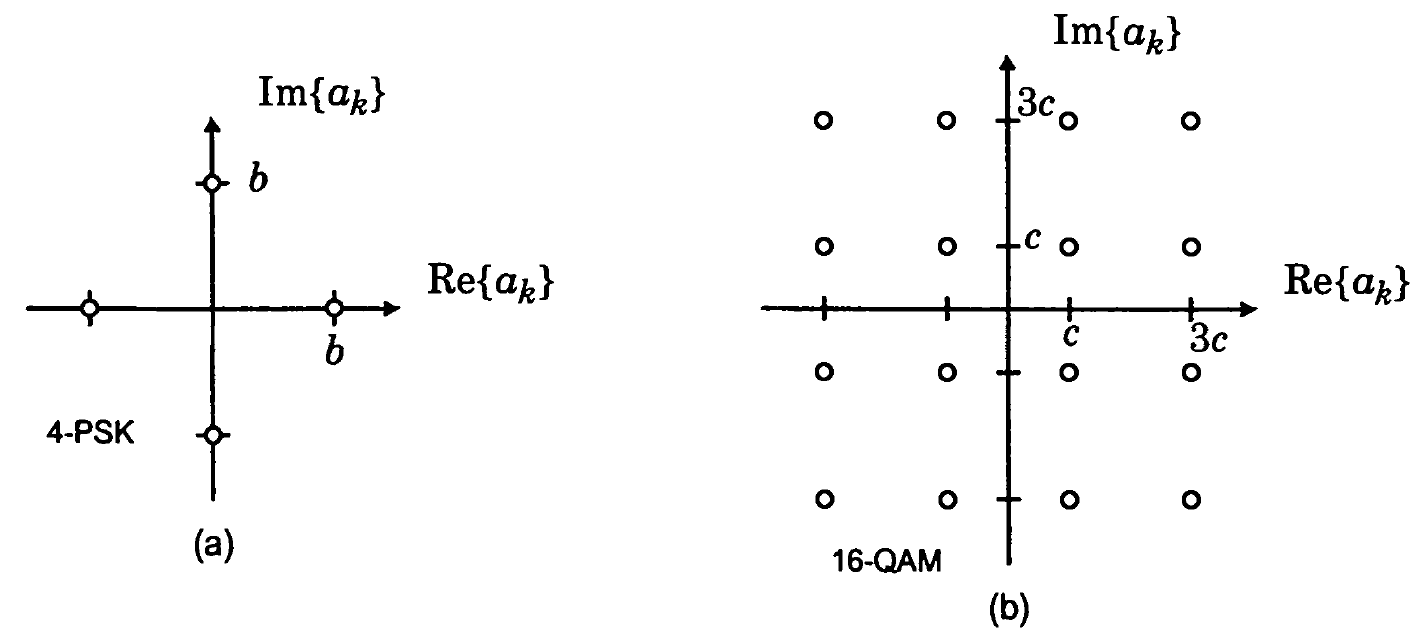
\includegraphics[width=0.7\columnwidth]{figs/pam_17}
	      \end{center}
	    \end{figure}
\end{frame}

\begin{frame}
	\frametitle{Constelações}

	\begin{itemize}
	    \item Cálculo da energia média de um pulso PAM em banda passante.
	    \item Considerações:
	    \begin{itemize}
		\item Símbolos equiprováveis.
		\item Pulso de transmissão $g(t)$ com energia $\mathcal{E}_g$.
		\item Pulso transmitido de forma \textbf{isolada}, por exemplo considerando pulso ideal de Nyquist com zero ISI. Neste caso pode-se omitir o subíndice $k$ relativo ao $k$-ésimo tempo de símbolo, ou seja, $\tilde{s}(t) = a g(t)$.
	    \end{itemize}
	    \item Sinal e seu equivalente passa-baixa: $s(t) = \sqrt{2} \mathrm{Re}\{ \tilde{s}(t) e^{j2\pi f_c t} \}$
	    \item Cálculo da energia média $\mathcal{E}$:
	    \begin{align*}
		\mathcal{E} &= \mathrm{E}\left[ \int_{-\infty}^{\infty} s^2(t) dt \right] = \mathrm{E} \left[ \int_{-\infty}^{\infty} |\tilde{s}(t)|^2 dt \right] = \mathrm{E}[|a|^2]\int_{-\infty}^{\infty} g^2(t) dt \\
		&= \left( \frac{1}{|\mathcal{A}|} \sum_{a \in \mathcal{A}} |a|^2 \right) \int_{-\infty}^{\infty} g^2(t) dt  =  \mathcal{E}_a \mathcal{E}_g
	    \end{align*}
	\end{itemize}	
\end{frame}

\begin{frame}
	\frametitle{Constelações}

	\begin{itemize}
	    \item Considerando a envoltória complexa $\tilde{s}(t)$ do sinal PAM, podemos calcular sua densidade espectral de potência (DEP) $S_{\tilde{s}}(f)$:
	    \begin{equation*}
		S_{\tilde{s}}(f) = \frac{1}{T}|G(f)|^2 S_{a}(f)
	    \end{equation*}
	    \item Onde $G(f)$ é a transformada de Fourier do pulso e $S_a(f)$ é a DEP da sequência de informação.
	    \item Para o caso em que a sequência é branca, a sua DEP é constante, dada por $S_a(f) = \mathcal{E}_a.$
	    \item A potência $P$ pode ser calculada ao integrar a DEP na frequência, obtendo portanto:
	    \begin{equation*}
		P = \int_{-\infty}^{\infty} \frac{1}{T} |G(f)|^2 S_a(f) df = \frac{\mathcal{E}_a}{T}\int_{-\infty}^{\infty} |G(f)|^2 df = \frac{\mathcal{E}_a\mathcal{E}_g}{T} = \frac{\mathcal{E}}{T}
	    \end{equation*}

	\end{itemize}	
\end{frame}

\begin{frame}
	\frametitle{Projeto da constelação}

	\begin{itemize}
	    \item A distância mínima $d_{\text{min}}$ é um parâmetro importante.
	    \item Quanto maior a distância mínima maior a imunidade ao ruído.
	    \item Relação custo-benefício entre potência de transmissão, tamanho da constelação e imunidade ao ruído.
	    \item Projeto da constelação:
	    \begin{itemize}
	      \item Objetivo: maximizar a distância entre símbolos evitando exceder a restrição de potência de transmissão.
	      \item Constelações ótimas podem ser difíceis de derivar e de alto custo.
	      \item Seu \textbf{desempenho} é invariante à translação.
	      \item Qual translação resulta em mínima potência?
	      \begin{equation*}
		\mathrm{E}[|a-m|^2] = \sum_{i=1}^M p_a(a_i) |a_i-m|^2
	      \end{equation*}
	      \item Melhor escolha para translação: $m = \mathrm{E}[a]$.
	      \item Constelação com média zero gasta menos energia que outras translações.
	    \end{itemize}	    	    
	\end{itemize}	
\end{frame}

\begin{frame}
	\frametitle{Projeto da constelação}

	\begin{itemize}
	    \item Exemplos de constelações QAM quadradas ($M=L^2$):
	    \begin{figure}[t]	
	    \begin{center}
	      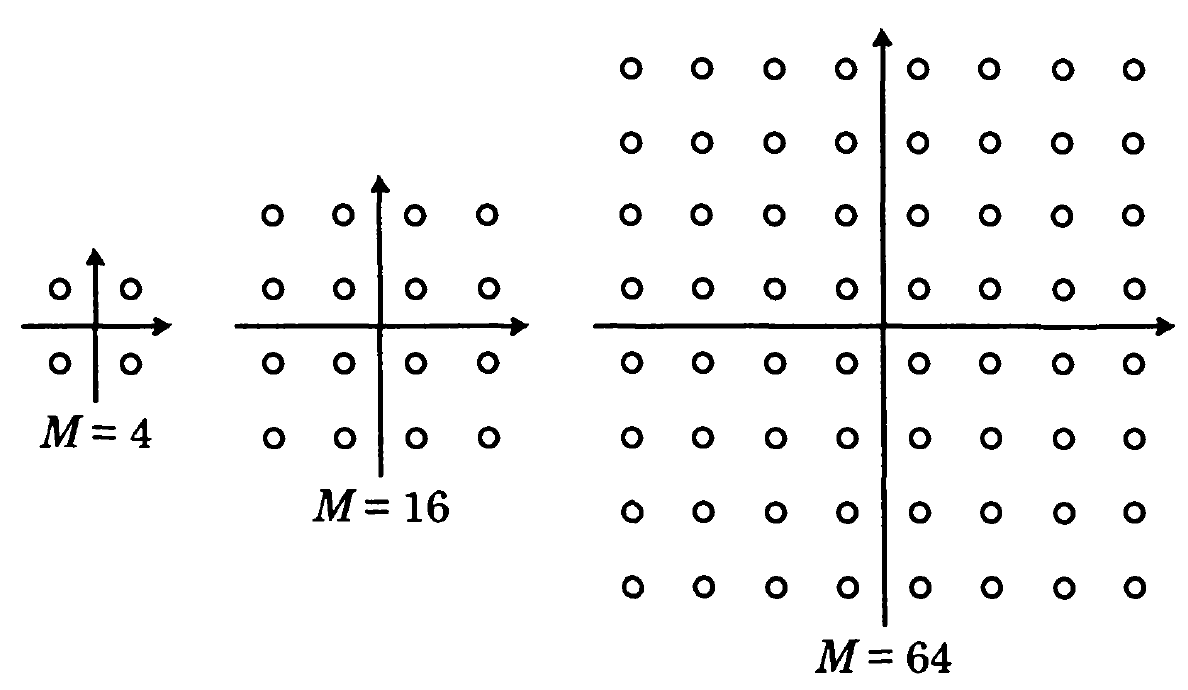
\includegraphics[width=0.45\columnwidth]{figs/pam_18}
	    \end{center}
	  \end{figure}
	    \item Componentes $a_I$ e $a_Q$ são escolhidas de um alfabeto PAM $L$-ário $\{ \pm c, \pm 3c, \ldots, \pm (L-1)c \}$, com $m$-ésimo elemento $c(-L+1+2m)$.
	    \item Energia média de uma constelação $M$-QAM:
	    \small
	    \begin{align*}
		  \mathcal{E}_a &= \mathrm{E}[|a|^2] = \mathrm{E}[a_I^2] + \mathrm{E}[a_I^2] = 2 \mathrm{E}[a_I^2] \\
		  &= \frac{2}{L}\sum_{m=0}^{L-1} c^2(-L+1+2m)^2 = \frac{2}{3}c^2(L^2-1) = \frac{2}{3}c^2(M-1)
	    \end{align*}
	\end{itemize}	
\end{frame}

\begin{frame}
	\frametitle{Projeto da constelação}

	\begin{itemize}
	    \item Exemplos de constelações QAM retangulares ($M\neq L^2$):
	    \begin{figure}[t]	
	    \begin{center}
	      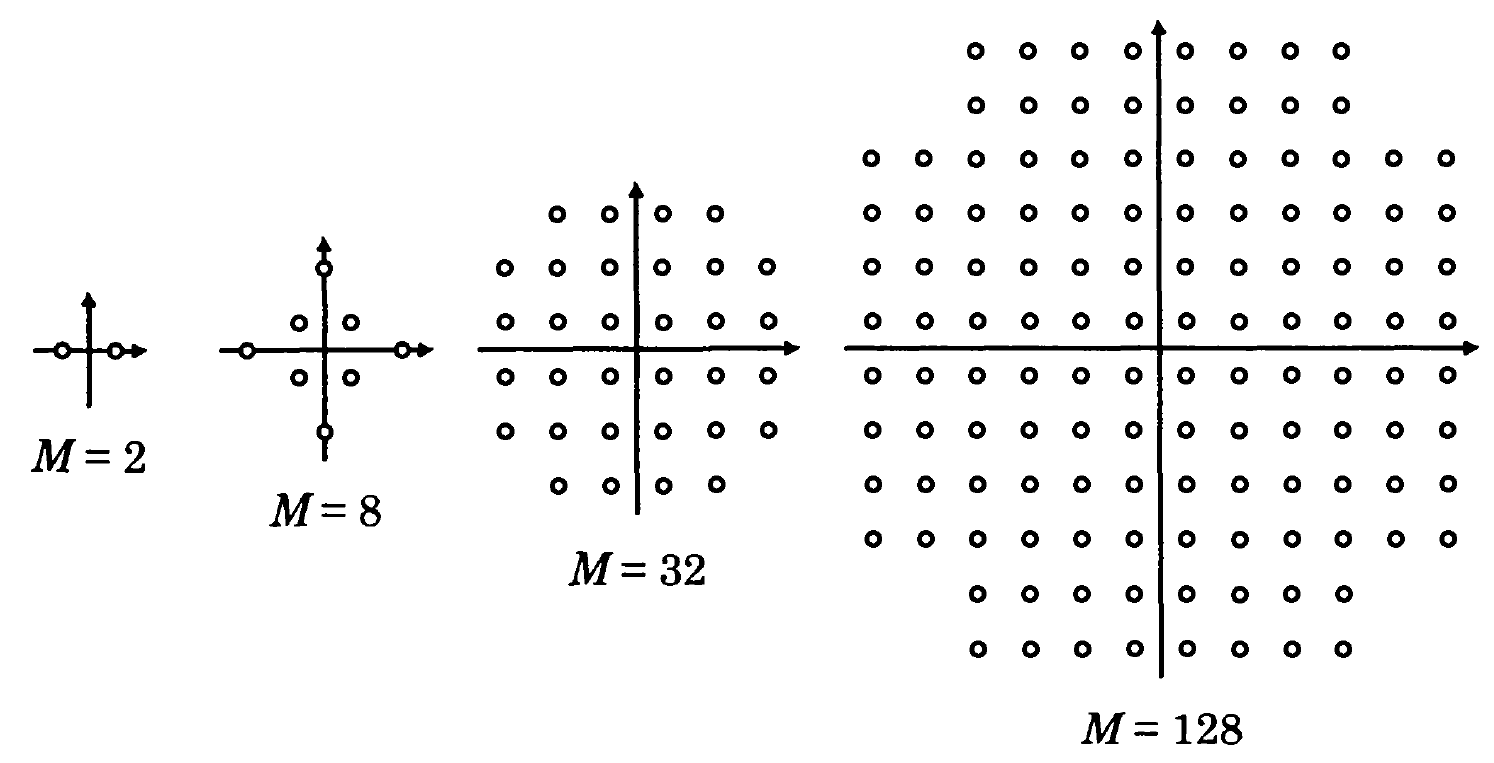
\includegraphics[width=0.55\columnwidth]{figs/pam_19}
	    \end{center}
	  \end{figure}
	    \item Mapeamento ligeiramente mais complicado.
	    \item Aplicações em combinação com códigos em treliça.
	\end{itemize}	
\end{frame}

\begin{frame}
	\frametitle{Projeto da constelação}

	\begin{itemize}
	    \item Exemplos de constelações PSK e AM-PM:
	    \begin{figure}[t]	
	    \begin{center}
	      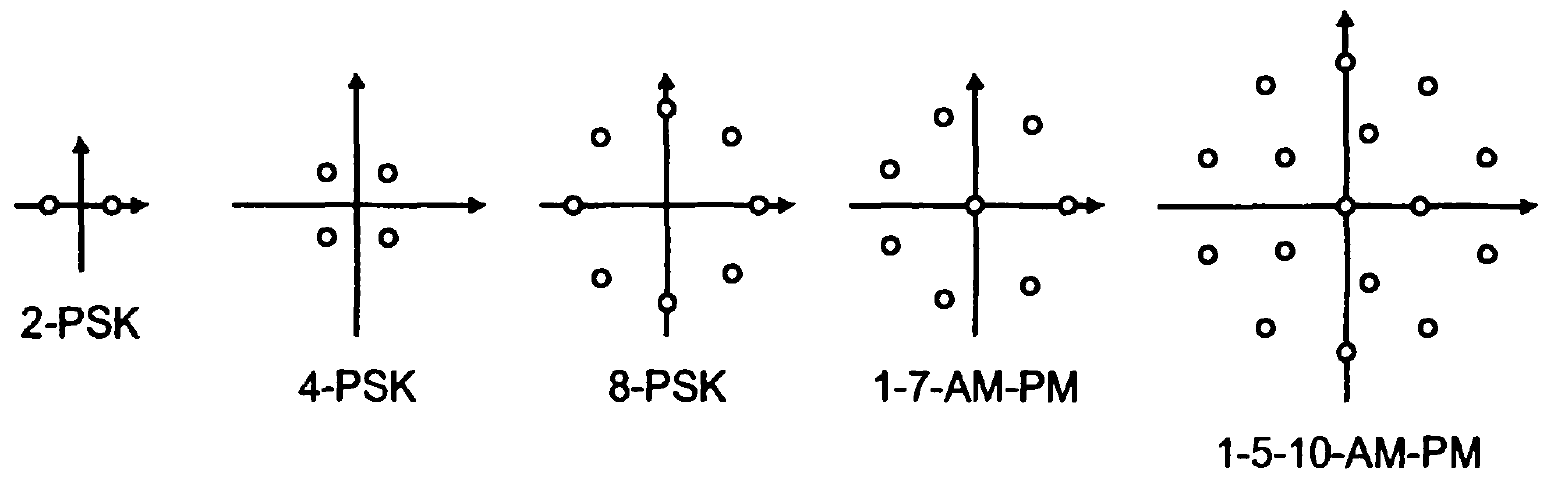
\includegraphics[width=0.7\columnwidth]{figs/pam_20}
	    \end{center}
	  \end{figure}
	    \item Elementos do alfabeto PSK: $a = \sqrt{\mathcal{E}} e^{j2\pi m/M}$
	    \item Envoltória constante e pontos com mesma energia.
	    \item Implementação de receptor de baixo custo.
	\end{itemize}	
\end{frame}

\begin{frame}
	\frametitle{Projeto da constelação}

	\begin{itemize}
	    \item Exemplos de constelações hexagonais:
	    \begin{figure}[t]	
	    \begin{center}
	      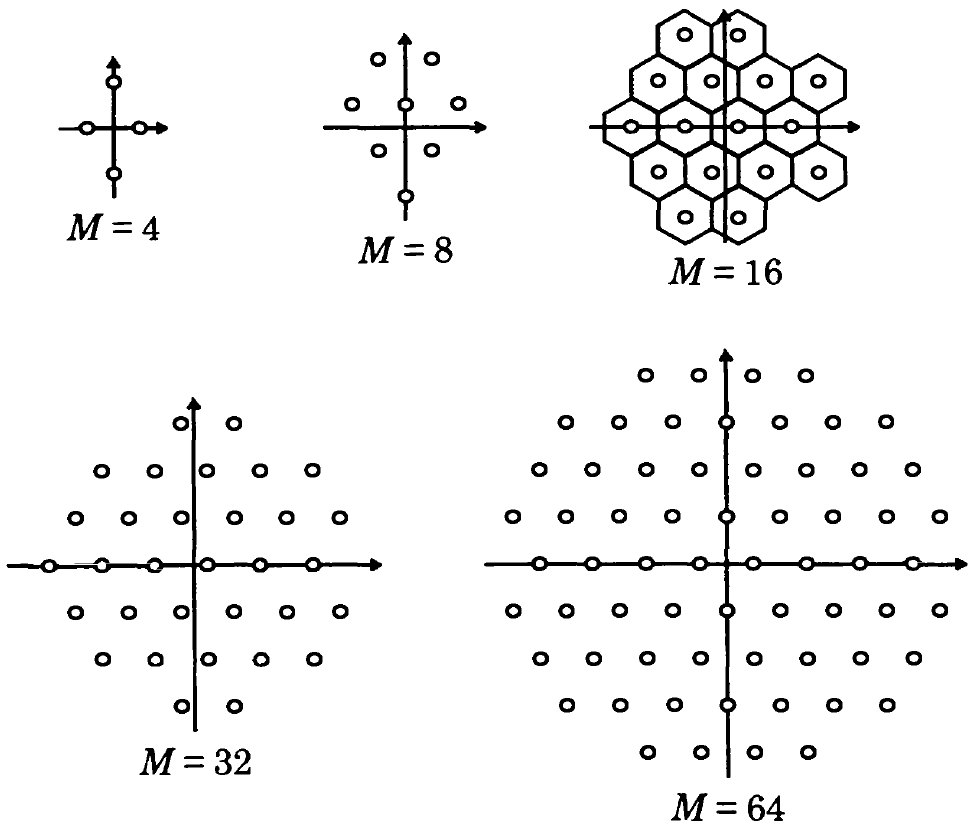
\includegraphics[width=0.45\columnwidth]{figs/pam_21}
	    \end{center}
	  \end{figure}
	    \item Símbolos localizados nos vértices de triângulos equiláteros.
	    \item Regiões de decisão hexagonais.
	    \item Desempenho ligeiramente superior a constelações retangulares, mas com complexidade elevada.
	\end{itemize}	
\end{frame}

\section{Receptor de distância mínima}

\begin{frame}
	\frametitle{Critério de distância mínima}

	\begin{itemize}
	    \item Mudamos agora o foco para o projeto do receptor.
	    \item Vamos considerar inicialmente a ausência de ISI, ou seja, assumindo que somente um pulso  é transmitido.
	    \item Projeto baseado em distância mínima e estrutura do filtro casado.
	    \item Expressão do sinal recebido considerando a transmissão de um único símbolo $a \in \mathcal{A}$:
	    \begin{equation*}
		r(t) = ah(t) + n(t)
	    \end{equation*}
	    \item Onde $h(t)$ é o pulso recebido e $n(t)$ é o ruído.
	    \item Modelo aplicável ao PAM em banda base ou em banda passante (foco no último caso, que é mais geral).
	    \item \textcolor{red}{Problema}: determinar a partir de $r(t)$ qual símbolo foi transmitido.
	\end{itemize}	
\end{frame}

\begin{frame}
	\frametitle{Critério de distância mínima}

	\begin{itemize}
	    \item Exemplo considerando sinalização binária antipodal, $\mathcal{A} = \{ -1, +1 \}$. 
	    \item Sina recebido sem ruído: $h(t)$ ou $-h(t)$
	\end{itemize}	
	\begin{columns}
		\begin{column}{0.5\textwidth}
		    \begin{figure}[t]	
		      \begin{center}
			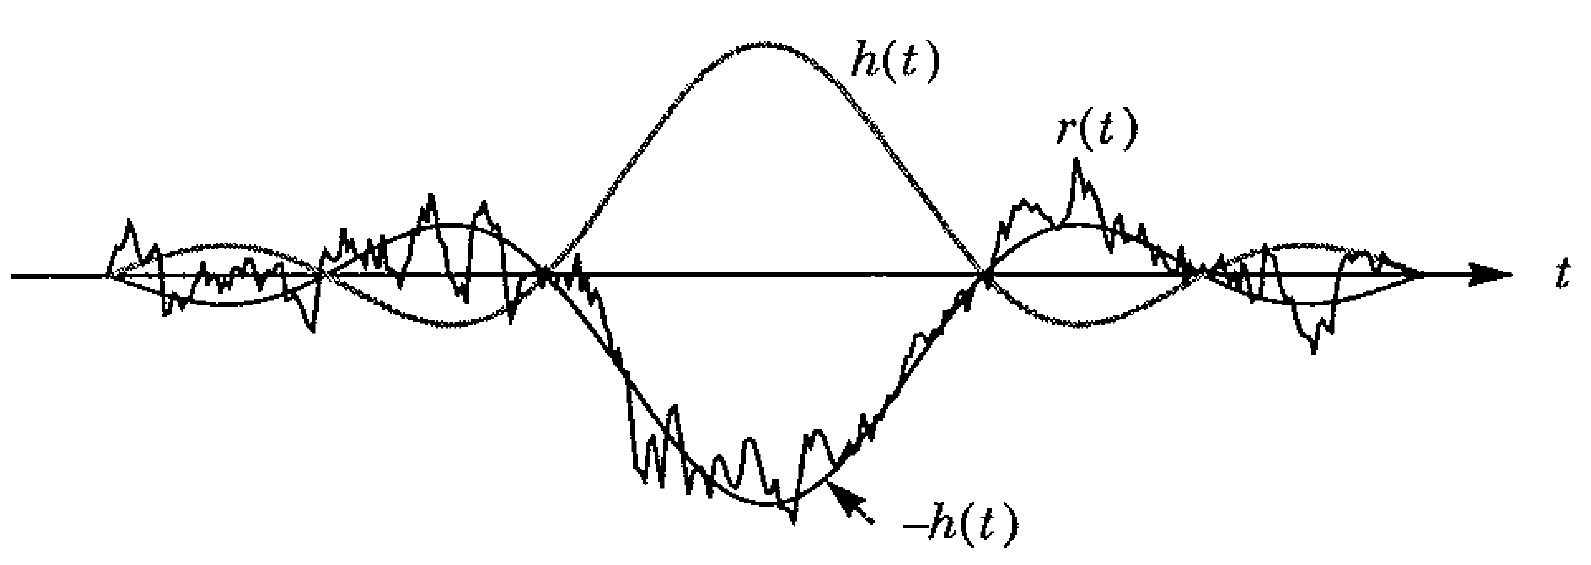
\includegraphics[width=\columnwidth]{figs/pam_23}
		      \end{center}\vspace{0.5cm}
		      \caption{Sinais antipodais e sinal recebido, dado que $-1$ foi transmitido.}
		    \end{figure}
		\end{column}
		\begin{column}{0.5\textwidth}
		     \begin{figure}[t]	
		      \begin{center}
			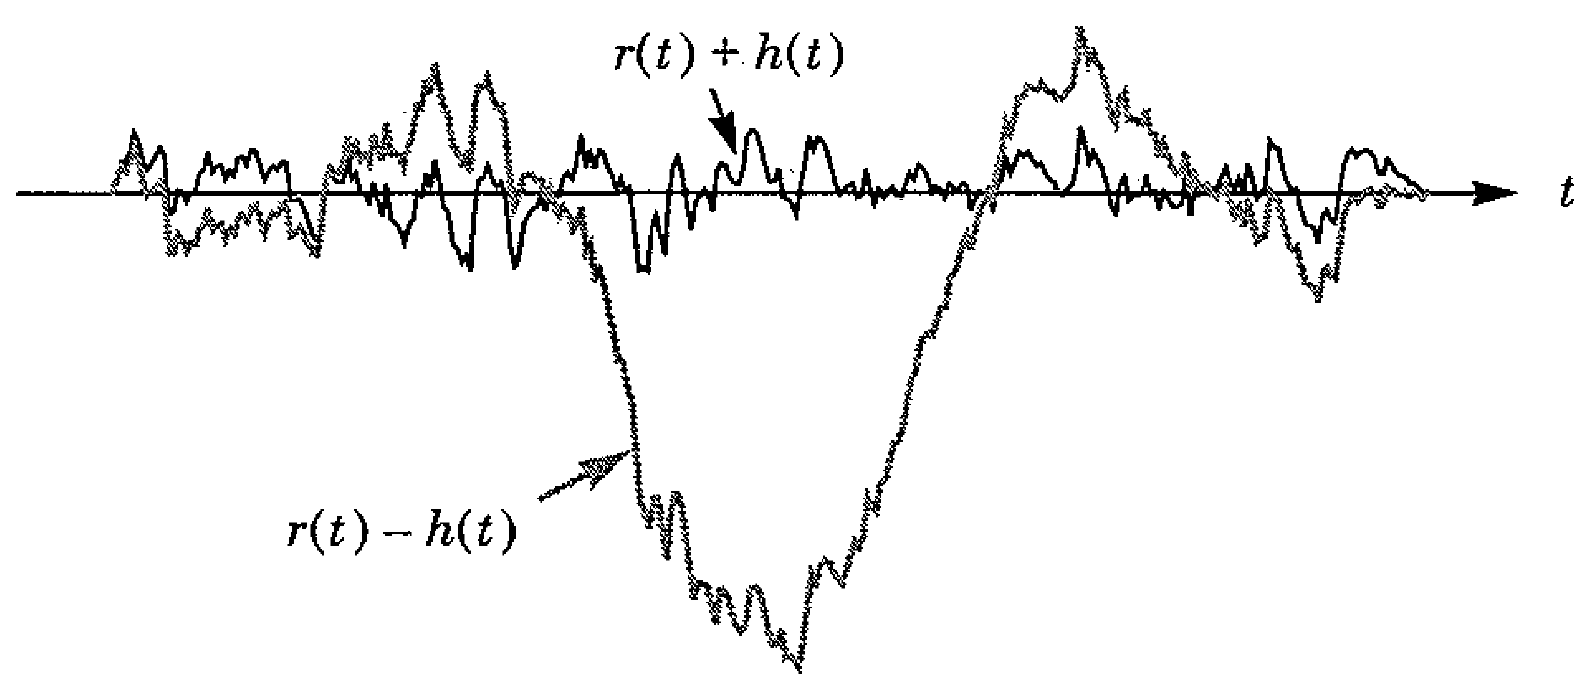
\includegraphics[width=\columnwidth]{figs/pam_24}
		      \end{center}
		      \caption{Diferença entre o sinal recebido e cada um dos sinais da constelação.}
		    \end{figure}
		\end{column}
	\end{columns}
	
\end{frame}

\begin{frame}
	\frametitle{Critério de distância mínima}

	\begin{itemize}
	    \item Quanto menor a diferença entre o sinal recebido e uma dada forma de onda, mais provável que esta tenha sido transmitida.
	    \item Essa métrica pode ser expressa como a energia do sinal da diferença:
	    \begin{equation*}
		\int_{-\infty}^{\infty} |r(t) -h(t)|^2 dt \quad \text{e} \quad \int_{-\infty}^{\infty} |r(t) +h(t)|^2 dt
	    \end{equation*}
	    \item O resultado é comparado e decide por $\hat{a}=1$ se a primeira energia for menor, ou por  $\hat{a}=-1$ se a segunda for menor.
	    \item De forma geral o \textbf{receptor de mínima distância} resolve o problema:
	    \begin{equation*}
		\hat{a} = \arg\min_{a\in \mathcal{A}} \int_{-\infty}^{\infty} |r(t) - ah(t)|^2 dt
	    \end{equation*}

	\end{itemize}			
\end{frame}

\begin{frame}
	\frametitle{Critério de distância mínima}

	\begin{itemize}
	    \item Análise da função custo $J$:
	    \begin{align*}
		J &= \int_{-\infty}^{\infty} |r(t) - ah(t)|^2 dt \\ &= \underbrace{\int_{-\infty}^{\infty} |r(t)|^2 dt}_{\mathcal{E}_r} - 2\mathrm{Re}\biggl\{ a^* \underbrace{\int_{-\infty}^{\infty} r(t)h^*(t) dt}_{y \, (\text{correlação})} \biggr\} + |a|^2 \underbrace{\int_{-\infty}^{\infty} |h(t)|^2 dt}_{\mathcal{E}_h}
% 		&=  - 2\mathrm{Re}\{ a^* y \} + |a|^2 \mathcal{E}_h
	    \end{align*}
	    \item Minimizar a distância equivale portanto a maximizar a correlação:
	    \begin{equation*}
		\hat{a} = \arg\max_{a\in \mathcal{A}} \, 2\mathrm{Re}\left\{ a^* \int_{-\infty}^{\infty} r(t) h^*(t) dt \right\} - |a|^2 \mathcal{E}_h
	    \end{equation*}
	    \item Implementação é simplificada, pois basta calcular uma vez a integral.
	\end{itemize}			
\end{frame}

\begin{frame}
	\frametitle{Critério de distância mínima}

	\begin{itemize}
	    \item Possíveis implementações da integral de correlação:
	\end{itemize}	
	\begin{columns}
		\begin{column}{0.45\textwidth}
		    \begin{figure}[t]	
		      \begin{center}
			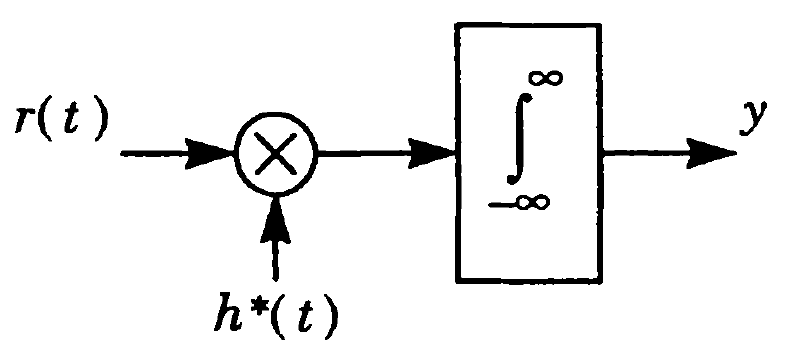
\includegraphics[width=0.75\columnwidth]{figs/pam_25}
		      \end{center}\vspace{-0.1cm}
		      \caption{Correlator.}
		    \end{figure}
		\end{column}
		\begin{column}{0.45\textwidth}
		     \begin{figure}[t]	
		      \begin{center}
			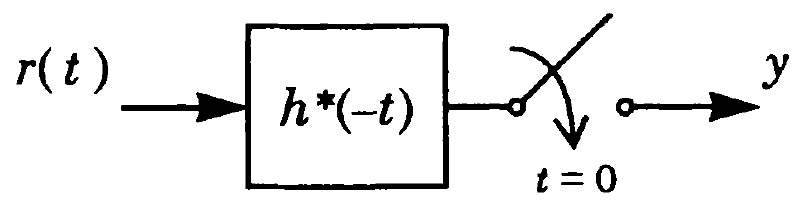
\includegraphics[width=0.85\columnwidth]{figs/pam_26}
		      \end{center}\vspace{0.5cm}
		      \caption{Filtro casado (MF).}
		    \end{figure}
		\end{column}
	\end{columns}
	\begin{itemize}
	    \item O MF é preferível ao correlator, pois permite compensar erros de sincronismo ao ajustar o instante de amostragem.
	\end{itemize}
\end{frame}

\begin{frame}
	\frametitle{Critério de distância mínima}

	\begin{itemize}
	    \item A função custo também pode ser reescrita como:
	    \begin{align*}
		J &= \mathcal{E}_h \left( \frac{\mathcal{E}_r}{\mathcal{E}_h} -2\mathrm{Re} \left\{ a^* \frac{y}{\mathcal{E}_h} \right\} + |a|^2 \right) = \mathcal{E}_h \left| \frac{y}{\mathcal{E}_h} - a  \right|^2 - \frac{|y|^2}{\mathcal{E}_h} + \mathcal{E}_r
	    \end{align*}
	    \item O que leva ao problema equivalente de distância mínima:
	    \begin{equation*}
		\hat{a} = \arg\min_{a \in \mathcal{A}} \left| \frac{y}{\mathcal{E}_h} - a \right|^2
	    \end{equation*}
	    \item Correlação normalizada $z = y / \mathcal{E}_h$
	    \item Decisão: quantização de $z$ para o símbolo mais próximo do alfabeto, também chamado de \textit{slicer}.
	    \begin{figure}[t]	
	    \begin{center}
	      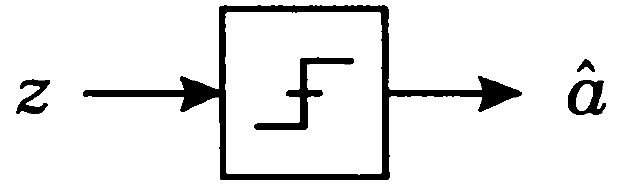
\includegraphics[width=0.25\columnwidth]{figs/pam_27}
	    \end{center} 
	  \end{figure}
	\end{itemize}		
\end{frame}

\begin{frame}
	\frametitle{Critério de distância mínima}

	\begin{itemize}
	    \item Resumo do esquema de recepção do PAM em banda passante:
	    \begin{figure}[t]	
	    \begin{center}
	      \includegraphics[width=0.8\columnwidth]{figs/pam_28}
	    \end{center} 
	  \end{figure}
	    \item Elementos: translação de frequência, filtro casado, amostragem, quantização (\textit{slicer}).
	    \item Para o PAM em banda base não é necessária a translação de frequência.
	\end{itemize}		
\end{frame}

\begin{frame}
	\frametitle{Propriedades do filtro casado}

	\begin{itemize}
	    \item O filtro casado representa uma forma de implementar o receptor de distância mínima.
	    \item Também pode ser demonstrado que \textcolor{blue}{o MF maximiza a SNR de recepção}.
	    \item Considere um filtro de recepção com resposta ao impulso $f(t)$. Segue a saída do filtro e sua posterior amostragem.
	    \begin{equation*}
		y(t) = \int_{-\infty}^{\infty} r(\tau)f(t-\tau)d\tau \; \xrightarrow{\text{amost. em } \; t=0} y(0) = \int_{-\infty}^{\infty} r(\tau)f(-\tau)d\tau
	    \end{equation*}
	    \item Substituindo $r(t)$ obtemos:
	    \begin{equation*}
		y = \underbrace{a \int_{-\infty}^{\infty} h(t) f(-t) dt}_{\textcolor{blue}{S}} + \underbrace{\int_{-\infty}^{\infty} n(t) f(-t) dt}_{\textcolor{red}{N}}
	    \end{equation*}

	\end{itemize}		
\end{frame}

\begin{frame}
	\frametitle{Propriedades do filtro casado}

	\begin{itemize}
	    \item Definição da relação sinal-ruído (SNR) no receptor:
	    \begin{equation*}
		SNR = \frac{\mathrm{E}[|S|^2]}{\mathrm{E}[|N|^2]} = \frac{\mathrm{E}[|a|^2]\left|\int h(t)f(-t)dt \right|^2}{N_0 \int |f(-t)|^2 dt} = \frac{\mathcal{E}_a \left|\int h(t)f(-t)dt \right|^2}{N_0 \mathcal{E}_f}
	    \end{equation*}
	    \item Considere a desigualdade de Schwarz: 
	    \begin{equation*}
		 \left| \int_{-\infty}^{\infty} u(t) v^*(t) dt \right|^2 \leq \int_{-\infty}^{\infty} |u(t)|^2 dt \int_{-\infty}^{\infty} |v(t)|^2 dt
	    \end{equation*}
	    \item O valor máximo é obtido para $v(t) = K u(t)$, onde $K$ é uma constante.
	    \item Aplicando a desigualdade para o numerador da SNR, obtemos o valor máximo para $f(t) = h^*(-t)$, resultando em
	    \begin{equation*}
		    SNR_{\text{max}} = \frac{\mathcal{E}_a \int |h(t)|^2 dt \int |f(t)|^2dt}{N_0 \mathcal{E}_f} = \frac{\mathcal{E}_a \mathcal{E}_h }{ N_0 }
	    \end{equation*}

	\end{itemize}
\end{frame}

\begin{frame}
	\frametitle{Filtro casado e ISI}

	\begin{itemize}
	    \item A otimização anterior desconsiderou o efeito da ISI.
	    \item A transmissão de uma sequência de pulsos geralmente introduz ISI.
	    \item Excessão para o caso em que o formato do pulso resultante obedece o critério de Nyquist.
	    \item A saída do filtro casado $h^*(-t)$ possui resposta em frequência $|H(f)|^2$.
	    \item O critério de Nyquist pode portanto ser expresso como:
	    \begin{equation*}
		    S_h(f) = \frac{1}{T} \sum_{m=-\infty}^{\infty} \left| H\left(f - \frac{m}{T} \right) \right|^2 = 1
	    \end{equation*}
	    \item O termo $S_h(f)$ é chamado de espectro dobrado (\textit{folded spectrum}) do pulso recebido.
	    \item Para cancelar a ISI pode ser aplicado um filtro de recepção raiz do cosseno levantado:
	    \begin{equation*}
		    H(f) = F(f) = P(f)^{1/2}
	    \end{equation*}

	\end{itemize}
\end{frame}

\begin{frame}
	\frametitle{Receptores PAM em banda passante}

	\begin{itemize}
	    \item Formas alternativas de implementação do PAM em banda passante:
	\end{itemize}
	\begin{figure}[t]	
	    \begin{center}
	    \includegraphics[width=0.5\columnwidth]{figs/pam_29}
	    \end{center} 
	\end{figure}
\end{frame}

\begin{frame}
	\frametitle{Receptores PAM em banda passante}

	\begin{itemize}
	    \item Receptores PAM mais elaborados:
	\end{itemize}
	\begin{figure}[t]	
	    \begin{center}
	    \includegraphics[width=0.9\columnwidth]{figs/pam_30}
	    \end{center} 
	\end{figure}
\end{frame}

\section{Detecção de sequência de distância mínima}

\begin{frame}
	\frametitle{Detecção de sequência de distância mínima}

	\begin{itemize}
	    \item Extensão do conceito de distância mínima para o caso ISI.
	    \item Sequência de $L$ símbolos: $ \mathcal{S} = \{ a_0, a_1, \ldots, a_{L-1} \}$, com $a_i \in \mathcal{A}$ e $M=|\mathcal{A}|$.
	    \item Expressão do sinal recebido:
	    \begin{equation*}
		r(t) = \sum_{k=0}^{L-1} a_k h(t-kT) + n(t)
	    \end{equation*}
	    \item Projeto do detector de sequência de distância mínima:
	    \begin{equation*}
		\hat{\mathcal{S}}_k = \arg \min_{\mathcal{S} \in \mathcal{A}^L} \int_{-\infty}^{\infty} \left| r(t) - \sum_{k=0}^{L-1} a_k h(t-kT) \right|^2 dt
	    \end{equation*}
	    \item Dentre as $M^L$ possíveis sequências, o receptor escolhe aquela que mais se aproxima do sinal observado $r(t)$.
	\end{itemize}	
\end{frame}

\begin{frame}
	\frametitle{Detecção de sequência de distância mínima}

	\begin{itemize}
	    \item A decisão é feita sobre toda a sequência, e não símbolo a símbolo.
	    \item Decisor deve esperar a chegada de todos os símbolos da sequência para tomar a decisão.
	    \item \textcolor{red}{Atraso} na decodificação é proporcional ao tamanho $L$ da sequência.
	    \item Conceito simples, mas \textcolor{red}{complexidade exponencial} em $L$.
	    \item Como tornar a implementação prática?
	\end{itemize}	
\end{frame}

\begin{frame}
	\frametitle{Detecção de sequência de distância mínima}

	\begin{itemize}
	    \item Reescrevendo a função custo:
	\end{itemize}	
	\begin{footnotesize}
	\begin{align*}
	    &J = \int_{-\infty}^{\infty} \left| r(t) - \sum_{k=0}^{L-1} a_k h(t-kT) \right|^2 dt \\
	    &= \mathcal{E}_r - 2\mathrm{Re}\Biggl\{ \sum_{k=0}^{L-1} a_k^* \underbrace{\int_{-\infty}^{\infty} \hspace{-0.15cm} r(t)h^*(t-kT) dt}_{y_k} \Biggr\} + \sum_{k=0}^{L-1} \sum_{j=0}^{L-1} a_k a_j^* \underbrace{\int_{-\infty}^{\infty} \hspace{-0.15cm} h(t-kT)h^*(t-jT) dt}_{\rho_h(j-k)} \\
	    &= \mathcal{E}_r - 2\mathrm{Re}\Biggl\{ \sum_{k=0}^{L-1} a_k^* y_k \Biggr\} + \sum_{k=0}^{L-1} \sum_{j=0}^{L-1} a_k a_j^* \rho_h(j-k)
	\end{align*}
	\end{footnotesize}
	\begin{itemize}
	    \item Problema equivalente a maximizar a correlação:
	    \begin{footnotesize}
	    \begin{equation*}
		\hat{\mathcal{S}}_k = \arg \max_{\mathcal{S} \in \mathcal{A}^L} \; 2\mathrm{Re}\Biggl\{ \sum_{k=0}^{L-1} a_k^* y_k \Biggr\} - \sum_{k=0}^{L-1} \sum_{j=0}^{L-1} a_k a_j^* \rho_h(j-k)
	    \end{equation*}
	    \end{footnotesize}
	\end{itemize}	
\end{frame}

\begin{frame}
	\frametitle{Detecção de sequência de distância mínima}

	\begin{itemize}
	    \item Correlações podem ser calculadas pelo filtro casado amostrado:
	    \begin{figure}[t]	
		\begin{center}
		\includegraphics[width=0.35\columnwidth]{figs/pam_31}
		\end{center} 
	    \end{figure}
	    \item Na presença de ISI o filtro casado acentua as distorções de canal.
	    \item Impacto do filtro casado e de equalizador sobre um pulso de recepção que não satisfaz o critério de Nyquist:
	    \begin{figure}[t]	
		\begin{center}
		\includegraphics[width=0.5\columnwidth]{figs/pam_32}
		\end{center} 
	    \end{figure}
	    \item Critério da distância mínima maximiza a SNR, mas não evita a ISI.
	\end{itemize}
\end{frame}

\begin{frame}
	\frametitle{Detecção de sequência de distância mínima}

	\begin{itemize}
	    \item Auto-correlação amostrada do pulso recebido: $\rho_h(k) = \langle h(t), h(t-kT) \rangle$
	    \item Propriedades de $\rho_h(k)$:
	    \begin{itemize}
		\item Valor em $k=0$ dado por $\rho_h(0) = \mathcal{E}_h$
		\item Simetria Hermitiana: $\rho_h(-k) = \rho_h^*(k)$
		\item Valor máximo em $\rho_h(0)$, ou seja, $|\rho_h(k)| \leq \rho_h(0) \, , \; \forall k$
		\item Auto-correlação amostrada pode ser vista como a saída de um filtro casado amostrado quando o pulso recebido é a entrada:
	    \end{itemize}
	    \begin{figure}[t]	
		\begin{center}
		\includegraphics[width=0.4\columnwidth]{figs/pam_33}
		\end{center} 
	    \end{figure}
	    \item Transformada discreta de Fourier da auto-correlação amostrada:
	    \begin{equation*}
		S_h(e^{j2\pi fT}) = \frac{1}{T} \sum_{m=-\infty}^{\infty} | H(f-m/T) |^2
	    \end{equation*}
	    \item Critério de Nyquist: $S_h(e^{j2\pi fT}) = \mathcal{E}_h$ e $\rho_h(k) = \mathcal{E}_h \delta_k$
	\end{itemize}
\end{frame}

\begin{frame}
	\frametitle{Estudo de caso: sinal NRZI}

	\begin{itemize}
	    \item Sinal com memória NRZI: \textit{non-return-to-zero, inverted}
	    \item Codificação diferencial, transições ocorrem quando $1$ é transmistido.
	    \item Sequência codificada de saída $\{b_k \}$, sequência de entrada $\{a_k \}$.	
	    \item Operação de codificação baseada em adição binária módulo 2.	    
	    \begin{equation*}
		b_k = a_k \oplus b_{k-1}
	    \end{equation*}
	    \begin{figure}[t]	
		\begin{center}
		\includegraphics[width=0.4\columnwidth]{figs/pam_35}
		\end{center} 
	    \end{figure}
	\end{itemize}
\end{frame}

\begin{frame}
	\frametitle{Estudo de caso: sinal NRZI}

	\begin{itemize}
	    \item Modelagem como cadeia de Markov de dois estados.
	    \item De forma geral, para o caso binário: $P[a_k=1]=1-P[a_k=0]=p$.
	    \item Matriz de transição de estados e diagrama correspondente:
	    \begin{columns}
		\begin{column}{0.35\textwidth}
		    \begin{equation*}
			\mathbf{P} = \left[ \begin{array}{cc} 1-p & p \\ p & 1-p \end{array} \right]
		    \end{equation*}
		\end{column}
		\begin{column}{0.65\textwidth}
		     \begin{figure}[t]	
		      \begin{center}
			\includegraphics[width=0.85\columnwidth]{figs/pam_36}
		      \end{center}
		    \end{figure}
		\end{column}
	    \end{columns}	 
	    \item Diagrama de treliça (evolução temporal):
	    \begin{figure}[t]	
	      \begin{center}
		\includegraphics[width=0.5\columnwidth]{figs/pam_37}
	      \end{center}
	    \end{figure}
	\end{itemize}
\end{frame}

\begin{frame}
	\frametitle{Algoritmo de Viterbi}

	\begin{itemize}
	    \item Considere um sinal PAM binário NRZI, com $s_1 = -s_2 = \sqrt{\mathcal{E}_b}$.
	    \item Número total de possíveis sequências $2^L$.
	    \item Algoritmo de Viterbi reduz a complexidade eliminando sequências de forma iterativa: algoritmo de busca em treliça.
	    \item Diagrama em treliça supondo estado inicial $S_0$.	    
	\end{itemize}
	\begin{figure}[t]	
	  \begin{center}
	    \includegraphics[width=0.5\columnwidth]{figs/pam_38}
	  \end{center}
	\end{figure}
\end{frame}

\begin{frame}
	\frametitle{Algoritmo de Viterbi}

	\vspace{-0.3cm}
	\begin{figure}[t]	
	  \begin{center}
	    \includegraphics[width=0.5\columnwidth]{figs/pam_38}
	  \end{center}\vspace{-0.5cm}
	\end{figure}
	\begin{itemize}
	    \item Memória de 1 bit, treliça atinge estado permanente após 2 transições.
	    \item Em $t=2T$ há dois caminhos entrando em cada nó.
	    \item Métricas de decisão para o nó $S_0$ baseadas em distância Euclidiana:
	    \begin{align*}
		D_0(0,0) &= (r_1 + \sqrt{\mathcal{E}_b})^2 + (r_2 + \sqrt{\mathcal{E}_b})^2 \\
		D_0(1,1) &= (r_1 - \sqrt{\mathcal{E}_b})^2 + (r_2 + \sqrt{\mathcal{E}_b})^2
	    \end{align*}
	    \item Caminho de menor métrica é escolhido e o outro é descartado.
	\end{itemize}
\end{frame}

\begin{frame}
	\frametitle{Algoritmo de Viterbi}

	\vspace{-0.3cm}
	\begin{figure}[t]	
	  \begin{center}
	    \includegraphics[width=0.5\columnwidth]{figs/pam_38}
	  \end{center}\vspace{-0.5cm}
	\end{figure}
	\begin{itemize}
	    \item Mesmo procedimento para o nó $S_1$ ainda em $t=2T$
	    \begin{align*}
		D_1(0,1) &= (r_1 + \sqrt{\mathcal{E}_b})^2 + (r_2 - \sqrt{\mathcal{E}_b})^2 \\
		D_1(1,0) &= (r_1 - \sqrt{\mathcal{E}_b})^2 + (r_2 - \sqrt{\mathcal{E}_b})^2
	    \end{align*}
	    \item Em $t=2T$ ficamos portanto com um caminho sobrevivente chegando em cada nó.
	\end{itemize}
\end{frame}

\begin{frame}
	\frametitle{Algoritmo de Viterbi}

	\vspace{-0.3cm}
	\begin{figure}[t]	
	  \begin{center}
	    \includegraphics[width=0.5\columnwidth]{figs/pam_38}
	  \end{center}\vspace{-0.5cm}
	\end{figure}
	\begin{itemize}
	    \item Supondo que os caminhos sobreviventes em $t=2T$ sejam $(0,0)$ em $S_0$ e $(0,1)$ em $S_1$.
	    \item As métricas em $t=3T$ são calculadas como:
	    \begin{small}
	    \begin{align*}
		D_0(0,0,0) &= D_0(0,0) + (r_3 + \sqrt{\mathcal{E}_b})^2 \qquad D_1(0,0,1) = D_0(0,0) + (r_3 - \sqrt{\mathcal{E}_b})^2 \\
		D_0(0,1,1) &= D_1(0,1) + (r_3 + \sqrt{\mathcal{E}_b})^2 \qquad D_1(0,1,0) = D_1(0,1) + (r_3 - \sqrt{\mathcal{E}_b})^2
	    \end{align*}
	    \end{small}
	    \item Novamente é escolhido o caminho de menor métrica em cada nó.
	\end{itemize}
\end{frame}

\begin{frame}
	\frametitle{Algoritmo de Viterbi}

	\begin{figure}[t]	
	  \begin{center}
	    \includegraphics[width=0.58\columnwidth]{figs/pam_40}
	  \end{center}
	\end{figure}
\end{frame}

\begin{frame}
	\frametitle{Algoritmo de Viterbi}

	\begin{itemize}
	    \item O processo continua a cada tempo de símbolo.
	    \item O número de caminhos na treliça é reduzido pela metade a cada estágio.
	    \item Pode ser generalizado para modulação $M$-ária.
	    \item A escolha do tamanho da sequência para realizar a decisão depende da memória (e.g., número de multi-percursos em canal rádio móvel).
	    \item Supondo que a memória tem comprimento $L_m$, uma implementação prática do algoritmo geralmente considera sequências de tamanho $L=5L_m$.
	    \item Desta forma é possível compensar o efeito da memória e evitar um atraso muito grande na entrega dos símbolos no receptor.
	\end{itemize}
\end{frame}

\begin{frame}
	\frametitle{Algoritmo de Viterbi}

	\begin{itemize}
	    \item Exemplo para 4-PSK, canal com memória de tamanho 2.
	\end{itemize}
	\begin{figure}[t]	
	  \begin{center}
	    \includegraphics[width=0.76\columnwidth]{figs/pam_39}
	  \end{center}
	\end{figure}
\end{frame}

% \begin{frame}
% 	\frametitle{Minimização da distância para tempo discreto}
% 
% 	\begin{itemize}
% 	    \item Cálculo direto do custo $J$ não é prático: 
% 	    \begin{itemize}
% 	     \item Para uma sequência requer por volta de $L^2$ operações e o número de sequências cresce exponencialmente com $L$.
% 	    \end{itemize}
% 	    \item Conversão do critério de distância mínima de tempo contínuo para tempo discreto:
% 	    \begin{figure}[t]	
% 		\begin{center}
% 		\includegraphics[width=0.75\columnwidth]{figs/pam_34}
% 		\end{center} 
% 	    \end{figure}
% 	    \item Problema equivalente:
% 	    \begin{equation*}
% 		\hat{\mathcal{S}}_k = \arg \max_{\mathcal{S} \in \mathcal{A}^L} \; \sum_{k=0}^{\infty} \left| z_k - \sum_{l=0}^{L-1} a_l m_{k-l} \right|^2
% 	    \end{equation*}
% 	\end{itemize}
% \end{frame}
% 
% \begin{frame}
% 	\frametitle{Minimização da distância para tempo discreto}
% 
% 	\begin{itemize}
% 	    \item Fatorização espectral
% 	    \begin{align*}
% 		&S_h(z) = \gamma^2 M(z) M^*(1/z^*) \\
% 		&\rho_h(k) = \gamma^2 m_k * m_{-k}^* \\
% 		&\text{Função de transferência do equalizador precursor: } \frac{1}{\gamma^2 M^*(1/z^*)} \\
% 		&y_k = \gamma^2 z_k * m_{-k}^* = \gamma^2 \sum_{l=k}^{\infty} z_l m_{l-k}^* \\
% 		
% 	    \end{align*}    
% 	\end{itemize}
% \end{frame}

\section{Análise de Desempenho em canais AWGN}

\begin{frame}
	\frametitle{Probabilidade de erro de símbolo}

	\begin{itemize}
	    \item Análise de desempenho do PAM em banda passante na presença de ruído aditivo Gaussiano branco (AWGN).
	    \item Considere um pulso PAM isolado (ou uma sequência de pulsos que satisfazem o critério de Nyquist).
	    \item Cadeia de transmissão e recepção:
	    \begin{figure}[t]	
	      \begin{center}
		\includegraphics[width=0.85\columnwidth]{figs/pam_41}
	      \end{center}
	    \end{figure}
	    \item Sinal recebido:
	    \begin{equation*}
		  r(t) = ah(t) + n(t)
	    \end{equation*}
	    \item Onde $a\in \mathcal{A}$, $h(t)$ é o pulso recebido e $n(t)$ o ruído recebido.
	\end{itemize}	
\end{frame}

\begin{frame}
	\frametitle{Probabilidade de erro de símbolo}

	\begin{itemize}
	    \item Caracterização estatística do ruído.
	    \item Considere que $n'(t)$ é o ruído antes da translação de frequência: real, Gaussiano, branco e com DEP $N_0/2$.
	    \begin{figure}[t]	
	      \begin{center}
		\includegraphics[width=0.45\columnwidth]{figs/pam_42}
	      \end{center}
	    \end{figure}
	    \item Cálculo da DEP do ruído filtrado em $v(t)$ e $n(t)$:
	    \begin{equation*}
		S_v(f) = (N_0/2)u(f) \qquad \text{e} \qquad S_n(f) = N_0u(f+f_c)
	    \end{equation*}
	    \item Considerando um receptor com filtro casado a saída terá DEP igual a $N_0 |H(f)|^2$.
	\end{itemize}	
\end{frame}

\begin{frame}
	\frametitle{Probabilidade de erro de símbolo}

	\begin{itemize}
	    \item Considerando o filtro casado, o sinal recebido normalizado é dado por:
	    \begin{align*}
		   z &= \mathcal{E}_h^{-1}\int_{-\infty}^{\infty} r(t) h^*(t) dt =  \mathcal{E}_h^{-1}\int_{-\infty}^{\infty} (ah(t) + n(t)) h^*(t) dt \\ &= a\mathcal{E}_h^{-1}\underbrace{\int_{-\infty}^{\infty} h(t) h^*(t) dt}_{\mathcal{E}_h} + \underbrace{\mathcal{E}_h^{-1}\int_{-\infty}^{\infty} n(t) h^*(t) dt}_{n} = a + n
	    \end{align*}
	    \item A variável complexa $n$ possui distribuição $\mathcal{CN}(0,N_0/\mathcal{E}_h)$
	    \item Processo similar pode ser aplicado para o PAM em banda base.
	\end{itemize}	
\end{frame}

\begin{frame}
	\frametitle{Probabilidade de erro de símbolo}

	\begin{itemize}
	    \item Relação sinal-ruído:
	    \begin{equation*}
		    \mathrm{SNR} = \frac{\mathrm{E}[|a|^2]}{\mathrm{E}[|n|^2]} = \frac{\mathcal{E}_a}{N_0/\mathcal{E}_h} = \frac{\mathcal{E}_a\mathcal{E}_h}{N_0}
	    \end{equation*}
	    \item Detecção: $z$ é aplicado a um \textit{slicer}, o qual escolher o símbolo $a \in \mathcal{A}$ que minimiza $|z-a|^2$.
	    \item Um \textbf{erro de símbolo} ocorre quando o \textit{slicer} escolhe um símbolo diferente daquele que foi de fato transmitido.
	    \item Vamos determinar a probabilidade de que o receptor de distância mínima cometa um erro de decisão em cenário AWGN.
	\end{itemize}	
\end{frame}

\begin{frame}
	\frametitle{Probabilidade de erro de símbolo}

	\begin{itemize}
	    \item Exemplo de detecção do \textcolor{blue}{BPSK}, para $\mathcal{A}=\{\pm \sqrt{\mathcal{E}_a} \}$
	    \item Supondo que o símbolo negativo foi transmitido, obtemos a PDF de $z$:
	    \begin{figure}[t]	
	      \begin{center}
		\includegraphics[width=0.6\columnwidth]{figs/pam_43}
	      \end{center}
	    \end{figure}
	    \item Distribuição de $z$: $\mathcal{N}(-\sqrt{\mathcal{E}_a},\sigma^2)$
	    \item Variância do ruído por dimensão: $\sigma^2 = N_0/(2\mathcal{E}_h)$
	    \item Distância entre símbolos: $d=2\sqrt{\mathcal{E}_a}$
	    \item Probabilidade de erro de símbolo:
	    \begin{equation*}
		    \mathrm{Pr[erro]} = Q(d/2\sigma) = Q(\sqrt{2\mathcal{E}/N_0})
	    \end{equation*}
	    \item Neste caso a probabilidade de erro de símbolo é igual à de erro de bit.
	\end{itemize}	
\end{frame}

\begin{frame}
	\frametitle{Probabilidade de erro de símbolo}

	\begin{itemize}
	    \item Exemplo de detecção do \textcolor{blue}{4-PAM}, para $\mathcal{A}=\{\pm c, \pm 3c \}$ e $c=\sqrt{\mathcal{E}_a/5}$
	    \item Supondo que o símbolo $-c$ foi transmitido, obtemos a PDF de $z$:
	    \begin{figure}[t]	
	      \begin{center}
		\includegraphics[width=0.43\columnwidth]{figs/pam_44}
	      \end{center}
	    \end{figure}
	    \item Cálculo da probabilidade de erro de símbolo:
	    \begin{footnotesize}
	    \begin{align*}
		    \text{Pr[erro}|a=\pm c] &= 2Q(d/2\sigma) \\
		    \text{Pr[erro}|a=\pm 3c] &= Q(d/2\sigma) \\
		    \mathrm{Pr}\text{[erro]} &= \frac{3}{2}Q(d/2\sigma) = \frac{3}{2}Q\left(\sqrt{\frac{2}{5}\mathcal{E}/N_0}\right)
	    \end{align*}
	    \end{footnotesize}
	    \item De forma geral, para o \textcolor{blue}{$M$-PAM} temos:
	    \begin{footnotesize}
	    \begin{align*}
		    \mathrm{Pr}\text{[erro]} &= \frac{2(M-1)}{M}Q\left(\sqrt{\frac{6}{(M^2-1)}\mathcal{E}/N_0}\right)
	    \end{align*}
	    \end{footnotesize}
	\end{itemize}	
\end{frame}

\begin{frame}
	\frametitle{Probabilidade de erro de símbolo}

	\begin{itemize}
	    \item Exemplo de detecção do \textcolor{blue}{4-QAM}, para $\mathcal{A}=\{\pm c \pm jc \}$ e $c=\sqrt{\mathcal{E}_a/2}$
	    \item Supondo que o símbolo $-c-jc$ foi transmitido:
	    \begin{figure}[t]	
	      \begin{center}
		\includegraphics[width=0.3\columnwidth]{figs/pam_45}
	      \end{center}
	    \end{figure}
	    \item Cálculo da probabilidade de erro de símbolo:
	    \begin{footnotesize}
	    \begin{align*}
		    &\text{Pr[acerto}|a=-c-jc] = \mathrm{Pr}[\mathrm{Re}\{z\}<0, \mathrm{Im}\{z\}<0] = (1-Q(d/2\sigma))^2 \\
		    &\text{Pr[erro]} = 1 - \text{Pr[acerto]} = 2Q(d/2\sigma) - Q^2(d/2\sigma) = 2Q(\sqrt{\mathcal{E}/N_0}) - Q^2(\sqrt{\mathcal{E}/N_0}) \\
		    &\text{Aproximação para altos valores de SNR: } \text{Pr[erro]}\approx 2Q(\sqrt{\mathcal{E}/N_0})
	    \end{align*}
	    \end{footnotesize}
	    \item O \textcolor{blue}{4-PSK}, para $\mathcal{A}=\{\pm b, \pm jb \}$ e $b=\sqrt{\mathcal{E}_a}$, corresponde a uma rotação de $45^o$ do 4-QAM, possuindo o mesmo desempenho.
	\end{itemize}	
\end{frame}

\begin{frame}
	\frametitle{Probabilidade de erro de símbolo}

	\begin{columns}
		\begin{column}{0.6\textwidth}
		    \begin{itemize}
			\item Exemplo de detecção do \textcolor{blue}{16-QAM}, para:
			\begin{footnotesize}
			\begin{align*}
			    \mathcal{A} &=\{\pm c \pm jc, \pm c \pm j3c, \pm 3c \pm jc, \pm 3c \pm j3c  \} \\ 
			    c &=\sqrt{\mathcal{E}_a/10}
			\end{align*}		
			\end{footnotesize}
			\item Definição de regiões: \begin{footnotesize}interna, canto, borda.\end{footnotesize}
		    \end{itemize}
		\end{column}
		\begin{column}{0.4\textwidth}
		    \begin{figure}[t]	
		    \begin{center}
			\includegraphics[width=0.8\columnwidth]{figs/pam_46}
		    \end{center}
		    \end{figure}
		\end{column}
	\end{columns}	
	\begin{itemize}
	    \item Cálculo da probabilidade de erro de símbolo:	    
	\end{itemize}	
	\begin{footnotesize}
	\begin{align*}
		&\text{Pr[acerto}|a \text{ interno}] = [1 - 2Q(d/2\sigma)]^2 &\Rightarrow \text{Pr[erro}|a \text{ interno}] \approx 4Q(d/2\sigma) \\
		&\text{Pr[acerto}|a \text{ canto}] = [1 - Q(d/2\sigma)]^2 &\Rightarrow \text{Pr[erro}|a \text{ canto}] \approx 2Q(d/2\sigma) \\
		&\text{Pr[acerto}|a \text{ borda}] = [1 - 2Q(d/2\sigma)][1 - Q(d/2\sigma)] &\Rightarrow \text{Pr[erro}|a \text{ borda}] \approx 3Q(d/2\sigma)
	\end{align*}
	\begin{align*}
		&\text{Pr[erro]} \approx \frac{4}{16}  4Q(d/2\sigma) + \frac{8}{16} 3Q(d/2\sigma) + \frac{4}{16} 2Q(d/2\sigma) = 3Q(d/2\sigma) = 3Q\left(\sqrt{\frac{\mathcal{E}}{5N_0}} \right)
	\end{align*}
	\end{footnotesize}	    
\end{frame}

\begin{frame}
	\frametitle{Probabilidade de erro de símbolo}

	\begin{itemize}
	    \item É possível derivar a expressão \textbf{exata} da probabilidade de erro de símbolo para constelações \textcolor{blue}{$M$-QAM} quadradas, nas quais $M=2^b$ para $b$ par.
	    \item Probabilidade de erro de símbolo do \textcolor{blue}{$\sqrt{M}$-PAM}, com metade da potência alocada em cada dimensão:
	    \begin{small}
	    \begin{equation*}
		\text{Pr[erro]}_{\sqrt{M}} = 2\left(1 - \frac{1}{\sqrt{M}} \right) Q\left(\sqrt{\frac{3\mathcal{E}/N_0}{M-1}} \right)
	    \end{equation*}
	    \item Probabilidade de erro de símbolo do \textcolor{blue}{$M$-QAM}:
	    \end{small}
	    \begin{small}
	    \begin{align*}
		\text{Pr[erro]}_M &= 1 - (1-\text{Pr[erro]}_{\sqrt{M}})^2 \\
		&= 4\left(1 - \frac{1}{\sqrt{M}} \right) Q\left(\sqrt{\frac{3\mathcal{E}/N_0}{M-1}} \right) - 4\left(1 - \frac{1}{\sqrt{M}} \right)^2 Q^2\left(\sqrt{\frac{3\mathcal{E}/N_0}{M-1}} \right) \\
		&\approx 4\left(1 - \frac{1}{\sqrt{M}} \right) Q\left(\sqrt{\frac{3\mathcal{E}/N_0}{M-1}} \right) \quad \text{(para altos valores de SNR)}
	    \end{align*}
	    \end{small}
	\end{itemize}		
\end{frame}

\begin{frame}
	\frametitle{Probabilidade de erro de símbolo}

	\begin{itemize}
	    \item Exemplo de detecção do \textcolor{blue}{$M$-PSK}, para $\mathcal{A}=\{c, ce^{j2\pi/M}, ce^{j4\pi/M}, \ldots, ce^{j2\pi(M-1)/M} \}$ e $c=\sqrt{\mathcal{E}_a}$
	\end{itemize}
	\begin{columns}
		\begin{column}{0.55\textwidth}
		    \begin{itemize}
			\item Região de decisão do símbolo $c$ entre $-\pi/M$ e $\pi/M$.
			\item Expressão fechada não pode ser encontrada.
			\item Cálculo da probabilidade de erro de símbolo:			
			\begin{align*}
			    &P_1 = \text{Pr}[\mathrm{Im}\{n'\} > d/2] = Q(d/2\sigma) \\
			    &n' = ne^{-j\pi/M}			    
			\end{align*}
		    \end{itemize}		    
		\end{column}
		\begin{column}{0.45\textwidth}
		    \begin{figure}[t]	
			\begin{center}\vspace{-0.5cm}
			    \includegraphics[width=\columnwidth]{figs/pam_47}
			\end{center}
			\end{figure}
		\end{column}
	\end{columns}	    	
	\begin{equation*}\hspace{-1.5cm}
	    \text{Pr[erro]} = 2P_1 - P_2 \approx 2Q(d/2\sigma) \approx2Q\left( \sqrt{2\mathcal{E}/N_0} \sin\frac{\pi}{M} \right)
	\end{equation*}	
\end{frame}


\begin{frame}
	\frametitle{Requisitos de banda e SNR do PAM em banda passante}

	\vspace{-0.3cm}
	\begin{itemize}
	    \item Probabilidade de erro de símbolo foi calculada como função da SNR = $\mathcal{E}/N_0$ para diferentes esquemas de modulação.
	    \item Para permitir a comparação entre esquemas de diferente ordens, é necessário normalizar a energia por bit:
	    \begin{equation*}
		\mathcal{E}_b = \mathcal{E}/\log_2 |\mathcal{A}| = \mathcal{E}/b
	    \end{equation*}
	    \item Razão entre a energia por bit e o ruído: $\mathcal{E}_b / N_0$
	    \item Mapeamento \textit{Gray} reduz a diferença entre símbolos adjacentes.
	\end{itemize}	
	\begin{columns}
		\begin{column}{0.5\textwidth}
		    \begin{itemize}			
			\item Aproximação:
			\begin{small}
			\begin{equation*}
			    \text{Pr[erro de bit]} \approx \frac{1}{b}\text{Pr[erro de símbolo]}
			\end{equation*}
			\end{small}
		    \end{itemize}		    
		\end{column}
		\begin{column}{0.5\textwidth}
		    \begin{figure}[t]	
			\begin{center}\vspace{-0.5cm}
			    \includegraphics[width=\columnwidth]{figs/pam_48}
			\end{center}
		    \end{figure}
		\end{column}
	\end{columns}	
\end{frame}

\begin{frame}
	\frametitle{Requisitos de banda e SNR do PAM em banda passante}

	\begin{itemize}
	    \item Expressões de probabilidade de erro de bit:
	    \begin{alignat*}{2}
		&P_b^{\text{BPSK}} &&= Q(\sqrt{2\mathcal{E}_b/N_0}) \\
		&P_b^{M-\text{QAM}} &&\approx \frac{4}{b} (1-2^{-b/2}) Q\left(\sqrt{\frac{3b\mathcal{E}_b/N_0}{2^b-1}} \right) \\
		&P_b^{M-\text{PSK}} &&\approx \frac{2}{b} Q\left(\sqrt{2b\mathcal{E}_b/N_0} \sin\frac{\pi}{M} \right)
	    \end{alignat*}

	\end{itemize}	
\end{frame}

\begin{frame}[t,fragile]
	\frametitle{Probabilidade de erro de símbolo}

	\begin{itemize}
	    \item Desempenho dos esquemas de modulação (QAM):
	\end{itemize}
	\begin{figure}\vspace{-0.4cm}
  \centering
    \begin{tikzpicture}
     \begin{axis}[
	    xlabel=$E_b/N_0$ em dB,
	    ylabel=Taxa de erro de bit,
	    ymode=log,
	    yminorticks=true,
 	    grid=major,
	    xmin=0, xmax=20, ymin=1e-4, ymax=1e0,
%   	    ytick={1-6,1e-5,...,1},
	    legend pos=outer north east,
	    legend cell align=left, font=\small,
	    height=6.7cm, width=0.8\columnwidth]
    \addplot[color=blue,mark=*, mark size=1.1pt, line width=1pt] table {
	     0.00000       7.8650e-02
	     2.00000       3.7506e-02
	     4.00000       1.2501e-02
	     6.00000       2.3883e-03
	     8.00000       1.9091e-04
	    10.00000       3.8721e-06
	    12.00000       9.0060e-09
	    14.00000       6.8102e-13
	    16.00000       2.2674e-19
	    18.00000       1.3960e-29
	    20.00000       1.0442e-45
    };
    \addplot[color=blue,mark=*, mark size=1.1pt, line width=1pt] table {
	     0.00000       7.8650e-02
	     2.00000       3.7506e-02
	     4.00000       1.2501e-02
	     6.00000       2.3883e-03
	     8.00000       1.9091e-04
	    10.00000       3.8721e-06
	    12.00000       9.0060e-09
	    14.00000       6.8102e-13
	    16.00000       2.2674e-19
	    18.00000       1.3960e-29
	    20.00000       1.0442e-45
    };
    \addplot[color=red,mark=*, mark size=1.1pt, line width=1pt] table {
	     0.00000       1.3916e-01
	     2.00000       9.7559e-02
	     4.00000       5.8618e-02
	     6.00000       2.7871e-02
 	     8.00000       9.2472e-03
	    10.00000       1.7542e-03
	    12.00000       1.3866e-04
	    14.00000       2.7632e-06
	    16.00000       6.2502e-09
	    18.00000       4.5223e-13
	    20.00000       1.4040e-19
    };
    \addplot[color=black,mark=*, mark size=1.1pt, line width=1pt] table {
	     0.00000       1.7295e-01
	     2.00000       1.4612e-01
	     4.00000       1.1576e-01
 	     6.00000       8.3473e-02
 	     8.00000       5.2320e-02
	    10.00000       2.6533e-02
	    12.00000       9.7240e-03
	    14.00000       2.1540e-03
	    16.00000       2.1717e-04
	    18.00000       6.3511e-06
	    20.00000       2.6339e-08
    };
    \addplot[color=green!60!black,mark=*, mark size=1.1pt, line width=1pt] table {
	     0.00000          1.7789e-01
	     2.00000          1.6391e-01
	     4.00000          1.4691e-01
 	     6.00000          1.2667e-01
 	     8.00000          1.0334e-01
	    10.00000          7.7807e-02
	    12.00000          5.2022e-02
	    14.00000          2.9098e-02
	    16.00000          1.2400e-02
	    18.00000          3.4721e-03
	    20.00000          5.0531e-04
    };    
    \legend{2-QAM, 4-QAM, 16-QAM, 64-QAM, 256-QAM};
     \end{axis}
     \end{tikzpicture}
     \end{figure}
\end{frame}

\begin{frame}[t,fragile]
	\frametitle{Probabilidade de erro de símbolo}

	\begin{itemize}
	    \item Desempenho dos esquemas de modulação (PSK):
	\end{itemize}
	\begin{figure}\vspace{-0.4cm}
  \centering
    \begin{tikzpicture}
     \begin{axis}[
	    xlabel=$E_b/N_0$ em dB,
	    ylabel=Taxa de erro de bit,
	    ymode=log,
	    yminorticks=true,
 	    grid=major,
	    xmin=0, xmax=20, ymin=1e-4, ymax=1e0,
%   	    ytick={1-6,1e-5,...,1},
	    legend pos=outer north east,
	    legend cell align=left, font=\small,
	    height=6.7cm, width=0.8\columnwidth]
    \addplot[color=blue,mark=*, mark size=1.1pt, line width=1pt] table {
	     0.00000       7.8650e-02
	     2.00000       3.7506e-02
	     4.00000       1.2501e-02
	     6.00000       2.3883e-03
	     8.00000       1.9091e-04
	    10.00000       3.8721e-06
	    12.00000       9.0060e-09
	    14.00000       6.8102e-13
	    16.00000       2.2674e-19
	    18.00000       1.3960e-29
	    20.00000       1.0442e-45
    };
    \addplot[color=blue,mark=*, mark size=1.1pt, line width=1pt] table {
	     0.00000       7.8650e-02
	     2.00000       3.7506e-02
	     4.00000       1.2501e-02
	     6.00000       2.3883e-03
	     8.00000       1.9091e-04
	    10.00000       3.8721e-06
	    12.00000       9.0060e-09
	    14.00000       6.8102e-13
	    16.00000       2.2674e-19
	    18.00000       1.3960e-29
	    20.00000       1.0442e-45
    };
    \addplot[color=green!60!black,mark=*, mark size=1.1pt, line width=1pt] table {
	     0.00000          1.1619e-01      
	     2.00000          7.9321e-02      
	     4.00000          4.5791e-02      
 	     6.00000          2.0480e-02      
 	     8.00000          6.1811e-03      
	    10.00000          1.0114e-03      
	    12.00000          6.3379e-05      
	    14.00000          8.7563e-07      
	    16.00000          1.1099e-09      
	    18.00000          3.2103e-14      
	    20.00000          2.3324e-21      
    }; 
    \addplot[color=red,mark=*, mark size=1.1pt, line width=1pt] table {
	     0.00000          1.4527e-01
	     2.00000          1.2181e-01
	     4.00000          9.5456e-02
	     6.00000          6.7726e-02
 	     8.00000          4.1432e-02
	    10.00000          2.0249e-02
	    12.00000          7.0096e-03
	    14.00000          1.4207e-03
	    16.00000          1.2460e-04
	    18.00000          2.9251e-06
	    20.00000          8.5726e-09
    };
    \addplot[color=black,mark=*, mark size=1.1pt, line width=1pt] table {
	     0.00000          0.144172
	     2.00000          0.138426
	     4.00000          0.131271
 	     6.00000          0.122417
 	     8.00000          0.111568
	    10.00000          0.098486
	    12.00000          0.083101
	    14.00000          0.065712
	    16.00000          0.047251
	    18.00000          0.029494
	    20.00000          0.014863
    };
    \legend{2-PSK, 4-PSK, 8-PSK, 16-PSK, 64-PSK};
     \end{axis}
     \end{tikzpicture}
     \end{figure}
\end{frame}

\begin{frame}
	\frametitle{Requisitos de banda e SNR do PAM em banda passante}

	\begin{itemize}
	    \item A SNR por bit necessária para alcançar um determinado valor de probabilidade de erro de bit pode ser encontrada ao rearranjar as equações anteriores:
	    \begin{align*}
		&(\text{QAM}): \mathcal{E}_b/N_0 = \underbrace{\frac{1}{3}\left(Q^{-1}\left( \frac{bP_b}{4(1-2^{-b/2})} \right) \right)^2}_{\Gamma \text{ (SNR gap)}} \underbrace{\left(\frac{2^b-1}{b}\right)}_{\text{Lim. de Shannon}}  \\ \\
		&(\text{PSK}): \mathcal{E}_b/N_0 = \frac{(Q^{-1}(bP_b/2))^2}{2b\sin^2\frac{\pi}{M}}
	    \end{align*}
	    \item Essas expressões quantificam os requisitos de potência, mas não de banda.
	\end{itemize}	
\end{frame}

\begin{frame}
	\frametitle{Requisitos de banda e SNR do PAM em banda passante}

	\begin{itemize}
	    \item Para o PAM em banda passante, considerando zero de banda de excesso, o requisito de banda é igual à taxa de símbolo. 
	    \item Requisito de banda normalizada: $1/b$
	    \item Comparação entre os esquemas de modulação ($P_b=10^{-6}$):
	    \begin{figure}[t]	
		\begin{center}
		    \includegraphics[width=0.95\columnwidth]{figs/pam_49}
		\end{center}
	    \end{figure}
	\end{itemize}	
\end{frame}

% \part{Modulações avançadas}
% \lecture{Modulações avançadas}{lec_advmod}

\begin{frame}
	\begin{block}{\centering\large\bfseries Parte 4}
		\centering\large\insertpart
	\end{block}
\end{frame}


\section{Modulação $M$-ária}

\begin{frame}
	\frametitle{Modulação $M$-ária}

	\begin{itemize}
	    \item Sinal modulado com PAM em banda base:
	    \begin{equation*}
		  s(t) = \sum_{k=-\infty}^{\infty} a_k g(t-kT)
	    \end{equation*}
	    \item Um único pulso $g(t)$ é utilizado e sua amplitude é modulada pelo símbolo de dados $a_k$.
	    \item O PAM pode ser generalizado para o caso de modulação $M$-ária considerando que o formato do pulso pode ser escolhido dentre $\{g_i(t) ; 0 \leq i \leq M-1 \}$. O sinal modulado é dado por:
	    \begin{equation*}
		  s(t) = \sum_{k=-\infty}^{\infty} g_{a_k}(t-kT)
	    \end{equation*}
	    \item Onde $a_k \in \{0, 1, \ldots, M-1 \}$. O símbolo de dados portanto indexa qual pulso é transmitido no $k$-ésimo intervalo de símbolo.
	\end{itemize}			
\end{frame}

\begin{frame}
	\frametitle{Modulação $M$-ária}

	\begin{itemize}
	    \item Exemplo para o 8-PAM.
	    \item Definição convencional: $\{ag(t) : a \in \mathcal{A} \}$ com $\mathcal{A} = \{\pm 1, \pm 3, \pm 5, \pm7 \}$.
	    \item Notação alternativa: $g_0(t)=-7g(t), g_1(t)=-5g(t),\ldots, g_7(t)=7g(t)$
	    \item Ilustração para um pulso retangular $g(t)$:
	    \begin{figure}[t]	
	      \begin{center}
		\includegraphics[width=0.75\columnwidth]{figs/adv_01}
	      \end{center}
	    \end{figure}
	\end{itemize}			
\end{frame}

\begin{frame}
	\frametitle{Modelo equivalente em banda base}

	\begin{itemize}
	    \item Relação entre sinal em banda passante $x(t)$ e sinal em banda base $s(t)$:
	    \begin{equation*}
		x(t) = \sqrt{2} \mathrm{Re}\{e^{j2\pi f_c t} s(t) \}
	    \end{equation*}
	    \item Similarmente para os pulsos em banda passante $\hat{g}(t)$ e banda base $g(t)$:
	    \begin{equation*}
		\hat{g}_i(t) = \sqrt{2} \mathrm{Re}\{e^{j2\pi f_c t} g_i(t) \}
	    \end{equation*}
	    \item Resultando no sinal em banda passante:
	     \begin{equation*}
		  x(t) = \sum_{k=-\infty}^{\infty} \hat{g}_{a_k}(t-kT)
	    \end{equation*}
	\end{itemize}			
\end{frame}

\begin{frame}
	\frametitle{Detecção de distância mínima}

	\begin{itemize}
	    \item Vamos considerar inicialmente a ausência de ISI, ou seja, assumindo que somente um pulso  é transmitido.
	    \item Um transmissor $M$-ário seleciona o sinal de $\{g_0(t), \ldots, g_{M-1}(t) \}$.
	    \item Supondo que $g_n(t)$ foi transmitido, o sinal recebido é dado por:
	    \begin{equation*}
		r(t) = h_n(t) + n(t)
	    \end{equation*}
	    \item Onde $h_n(t)$ é o $n$-ésimo pulso recebido e $n(t)$ é o ruído. Considerando que $b(t)$ é a resposta ao impulso do canal, temos:
	    \begin{equation*}
		H_n(f) = G_n(f)B(f+f_c)
	    \end{equation*}
	    \item Essa abordagem é válida para os casos em banda base e banda passante.
	\end{itemize}
\end{frame}

\begin{frame}
	\frametitle{Detecção de distância mínima}

	\begin{itemize}
	    \item Detector de distância mínima: escolhe o símbolo que melhor se aproxima ao sinal recebido.
	    \item Pode ser generalizado para o caso de modulação $M$-ária.
	    \item Função custo a ser \textcolor{blue}{minimizada}:
	    \begin{footnotesize}
	    \begin{equation*}
		J = \int_{-\infty}^{\infty} |r(t) - h_i(t)|^2 dt = \underbrace{\int_{-\infty}^{\infty} |r(t)|^2 dt}_{\mathcal{E}_r} - 2 \underbrace{\mathrm{Re}\left\{\int_{-\infty}^{\infty} r(t)h_i^*(t) dt \right\}}_{y_i} + \underbrace{\int_{-\infty}^{\infty} |h_i(t)|^2 dt}_{\mathcal{E}_i}
	    \end{equation*}
	    \end{footnotesize}
	    \item De forma análoga, o problema é equivalente a \textcolor{blue}{maximizar}:
	    \begin{equation*}
		 J_i = y_i - \frac{1}{2}\mathcal{E}_i
	    \end{equation*}
	    \item O que corresponde ao receptor de correlação.
	\end{itemize}
\end{frame}

\begin{frame}
	\frametitle{Detecção de distância mínima}

	\begin{itemize}
	    \item Ilustração do receptor de correlação:
	    \begin{figure}[t]	
	      \begin{center}
		\includegraphics[width=0.85\columnwidth]{figs/adv_02}
	      \end{center}
	    \end{figure}
	    \item O sinal recebido é correlacionado com os $M$ possíveis pulsos utilizando um banco de filtros casados amostrados.
	\end{itemize}
\end{frame}

\begin{frame}
	\frametitle{Detecção de distância mínima}

	\begin{itemize}
	    \item Variação do receptor de correlação utilizando correlatores no lugar de filtros casados.
	    \begin{figure}[t]	
	      \begin{center}
		\includegraphics[width=0.7\columnwidth]{figs/adv_03}
	      \end{center}
	    \end{figure}
	    \item Adequado para cenário em banda base.
	\end{itemize}
\end{frame}

\begin{frame}
	\frametitle{Detecção de distância mínima}

	\begin{itemize}
	    \item Complexidade do receptor de correlação é dominada pelas $M$ correlações que devem ser computadas.
	    \item Motivação para se desenvolver um método de menor complexidade.
	    \item Seja $\mathcal{S} = \mathrm{span}\{h_0(t),\ldots,h_{M-1}(t) \}$ o \textcolor{blue}{espaço de sinal} e seja $\hat{r}(t)$ a projeção de $r(t)$ em $\mathcal{S}$.
	    \item Como o erro de projeção $r(t)-\hat{r}(t)$ é ortogonal a $\mathcal{S}$, temos:
	    \begin{align*}
		J &= \int_{-\infty}^{\infty}|r(t) - \hat{r}(t) + \hat{r}(t) - h_i(t)|^2 dt \\
		&= \int_{-\infty}^{\infty}|r(t) - \hat{r}(t)|^2 dt + \int_{-\infty}^{\infty}|\hat{r}(t) - h_i(t)|^2 dt
	    \end{align*}
	    \item O problema de otimização se reduz a minimizar:
	    \begin{equation*}
		J' = \int_{-\infty}^{\infty} |\hat{r}(t) - h_i(t)|^2 dt
	    \end{equation*}

	\end{itemize}
\end{frame}

\begin{frame}
	\frametitle{Detecção de distância mínima}

	\begin{itemize}
	    \item Seja $\{\phi_1(t),\ldots,\phi_N(t) \}$ uma base ortonormal para $\mathcal{S}$.
	    \item Pode-se utilizar o método de Gram-Schmidt sobre $\{h_0(t),\ldots,h_{M-1}(t) \}$.
	    \item Seja $\mathbf{h}_i = [h_{i,1}, h_{i,2},\ldots,h_{i,N}]^T$ o vetor de coeficientes da projeção de $h_i(t)$, onde:
	    \begin{equation*}
		h_{i,j} = \int_{-\infty}^{\infty} h_i(t)\phi_j^*(t) dt
	    \end{equation*}
	    \item O custo de distância mínima se reduz a:
	    \begin{equation*}
		J' = || \mathbf{r} - \mathbf{h}_i ||^2
	    \end{equation*}
	    \item Onde $\mathbf{r} = [r_1,\ldots,r_N]^T$ é o vetor projeção de $r(t)$, com:
	    \begin{equation*}
		r_j = \int_{-\infty}^{\infty} r(t)\phi_j^*(t) dt
	    \end{equation*}
	\end{itemize}
\end{frame}

\begin{frame}
	\frametitle{Detecção de distância mínima}

	\begin{itemize}
	    \item Forma alternativa de implementar o receptor de distância mínima: \textbf{Receptor de projeção}.    
	    \begin{figure}[t]	
	      \begin{center}
		\includegraphics[width=0.75\columnwidth]{figs/adv_04}
	      \end{center}
	    \end{figure}
	    \item Complexidade reduzida de $M$ (tamanho da constelação) para $N$ (tamanho do espaço de sinal).
	\end{itemize}
\end{frame}

\section{Probabilidade de erro}

\begin{frame}
	\frametitle{Desempenho em cenário AWGN}

	\begin{itemize}
	    \item A $i$-ésima componente da projeção do sinal recebido é dada por:
	    \begin{equation*}
		    r_j = \underbrace{\int_{-\infty}^{\infty} h_i(t)\phi_j^*(t) dt}_{h_{i,j}} + \underbrace{\int_{-\infty}^{\infty} n(t)\phi_j^*(t) dt}_{n_j}
	    \end{equation*}
	    \item Considerando o vetor do ruído projetado $\mathbf{n}=[n_1,\ldots,n_N]^T$, temos:
	    \begin{equation*}
		    \mathbf{r} = \mathbf{h}_i + \mathbf{n}
	    \end{equation*}
	    \item $n(t)$ é a envoltória complexa do ruído Gaussiano branco em banda passante $\hat{n}(t)$. A DEP de $\hat{n}(t)$ é $N_0/2$ e a DEP de $n(t)$ é $N_0$.
	    \item Os $M$ vetores $\{\mathbf{h}_1,\ldots,\mathbf{h}_M \}$ são chamados de \textcolor{blue}{vetores de sinal}.
	\end{itemize}
\end{frame}

\begin{frame}
	\frametitle{Desempenho em cenário AWGN}

	\begin{itemize}
	    \item Podemos mostrar que as componentes do vetor $\mathbf{n}$ são i.i.d. com distribuição $\mathcal{CN}(0,N_0)$.
	    \item As componentes possuem média zero e a autocorrelação é dada por:
	    \begin{align*}
		\mathrm{E}[n_i n_j^*] = \mathrm{E}\left[\int_{-\infty}^{\infty} n(t)\phi_i^*(t) dt  \int_{-\infty}^{\infty} n^*(\tau)\phi_j(\tau) d\tau \right] = N_0 \delta_{i,j}
	    \end{align*}
	    \item Foram usadas as propriedades: linearidade da esperança, autocorrelação de $n(t)$ dada por $N_0\delta(t-\tau)$, e funções $\phi$ ortogonais entre si.
	    \item A matriz de autocorrelação de $\mathbf{n}$ é portanto diagonal.
	\end{itemize}
\end{frame}

\begin{frame}
	\frametitle{Desempenho em cenário AWGN}

	\begin{itemize}
	    \item Propriedades do vetor de ruído $\mathbf{n}$:
	    \begin{itemize}
		\item As $2N$ V.A.s reais $\{\mathrm{Re}\{n_1\},\ldots,\mathrm{Re}\{n_N\},\mathrm{Im}\{n_1\},\ldots,\mathrm{Im}\{n_N\} \}$ são mutuamente independentes, com média zero e variância $N_0/2$.
		\item O vetor $\mathbf{n}$ é circularmente simétrico e Gaussiano, com média zero e $\mathrm{E}[\mathbf{nn}^*] = N_0 \mathbf{I}$.
		\item Os componentes de $\mathbf{n}$ são descorrelacionados, $\mathrm{E}[n_in_j^*]=0$ para $i\neq j$.
		\item Os componentes de $\mathbf{n}$ são circularmente simétricos, $\mathrm{E}[n_in_j]=0$ para $1 \leq i, \; j\leq N$.
		\item Seja a variável aleatória $X = \langle \mathbf{n}, \mathbf{e} \rangle = \mathbf{e}^* \mathbf{n}$, ela será $\mathcal{CN}(0,N_0)$ para qualquer vetor $\mathbf{e}$ de norma unitária.
	    \end{itemize}
	\end{itemize}
\end{frame}

\begin{frame}
	\frametitle{Desempenho em cenário AWGN}

	\begin{itemize}
	    \item Normalmente não é possível encontrar o valor exato da probabilidade de erro do receptor de distância mínima.
	    \item Limitantes podem ser calculados para a probabilidade de erro.
	    \item \textcolor{blue}{Probabilidade de erro em pares} ($P_{i\rightarrow j}$):
	    \begin{itemize}
		\item Probabilidade de que o sinal recebido esteja mais próximo de $\mathbf{h}_j$ do que de $\mathbf{h}_i$, dado que $\mathbf{h}_i$ foi transmitido, para $j\neq i$.
	    \end{itemize}
	    \begin{align*}
		P_{i\rightarrow j} &= \mathrm{Pr}\left[ || \mathbf{r} - \mathbf{h}_j ||^2 < || \mathbf{r} - \mathbf{h}_i ||^2 \mid \mathbf{h}_i \text{ foi transmitido} \right] \\
		&= \mathrm{Pr}\left[ || \mathbf{n} - (\mathbf{h}_j - \mathbf{h}_i) ||^2 < || \mathbf{n} ||^2 \right] \\
		&= \mathrm{Pr}\Bigl[ || \mathbf{n} ||^2 + \underbrace{|| \mathbf{h}_j - \mathbf{h}_i ||^2}_{d_{i,j}^2} - 2\mathrm{Re}\{ \langle \mathbf{n}, \mathbf{h}_j - \mathbf{h}_i \rangle \} < || \mathbf{n} ||^2 \Bigr] \\
		&= \mathrm{Pr}\left[ \mathrm{Re}\{ \langle \mathbf{n}, (\mathbf{h}_j - \mathbf{h}_i)/d_{i,j} \rangle \} > d_{i,j}/2 \right] = Q\left(\frac{d_{i,j}}{2\sigma} \right)
	    \end{align*}
	\end{itemize}
\end{frame}

\begin{frame}
	\frametitle{Desempenho em cenário AWGN}

	\begin{itemize}
	    \item Comparação entre diferentes esquemas de modulação binária com mesma energia média $\mathcal{E}$.
	    \begin{figure}[t]	
	      \begin{center}
		\includegraphics[width=0.65\columnwidth]{figs/adv_05}
	      \end{center}
	    \end{figure}
	    \item Sinalização antipodal: $d=2\sqrt{\mathcal{E}}$ e $P_e = Q(\sqrt{2\mathcal{E}/N_0})$
	    \item Sinalização OOK e ortogonal: $d=\sqrt{2\mathcal{E}}$ e $P_e = Q(\sqrt{\mathcal{E}/N_0})$
	    \item Vantagem de 3dB para a sinalização antipodal.
	\end{itemize}
\end{frame}

\begin{frame}
	\frametitle{Desempenho em cenário AWGN}

	\begin{itemize}
	    \item \textcolor{blue}{Limitante da união}: limitante superior para a probabilidade de erro.
	    \item De forma geral, para $N$ eventos de erro $\{ \mathpzc{E}_n, 1 \leq n \leq N \}$ temos
	    \begin{equation*}
		\mathrm{Pr}\left[ \bigcup_{n=1}^N \mathpzc{E}_n \right] \leq \sum_{n=1}^N \mathrm{Pr}[\mathpzc{E}_n] 
	    \end{equation*}
	    \item Considerando que $\mathbf{h}_0$ foi transmitido, podemos definir $\mathpzc{E}_j$ como o evento de erro no qual $\mathbf{h}_j$ é escolhido no lugar de $\mathbf{h}_0$, ou seja, $P_{0\rightarrow j} = \mathrm{Pr}[\mathpzc{E}_j]$.
	    \item Podemos então calcular o limitante superior:
	    \begin{align*}
		\mathrm{Pr}[\text{erro} \mid \mathbf{h}_0 \text{ foi transmitido}] &=  \mathrm{Pr}\left[ \bigcup_{j=1}^{M-1} \mathpzc{E}_j \right] \leq \sum_{j=1}^{M-1} \mathrm{Pr}[\mathpzc{E}_j] \\
		\mathrm{Pr}[\text{erro} \mid \mathbf{h}_0 \text{ foi transmitido}] &\leq \sum_{j=1}^{M-1} Q\left(\frac{d_{0,j}}{2\sigma} \right)
	    \end{align*}	    
	\end{itemize}
\end{frame}

\begin{frame}
	\frametitle{Desempenho em cenário AWGN}

	\begin{itemize}
	    \item O limitante inferior pode ser obtido considerando a probabilidade de um único evento $\mathpzc{E}_m$, para $1\leq m \leq M-1$.
	    \item Para que o limitante seja mais representativo, podemos considerar um evento de erro que tenha a mínima distância para o sinal transmitido.
	    \begin{equation*}
		 \mathrm{Pr}\left[ \bigcup_{j=1}^{M-1} \mathpzc{E}_j \right] \geq \mathrm{Pr}[\mathpzc{E}_{\min}] = Q\left(\frac{d_{0,\min}}{2\sigma} \right)
	    \end{equation*}
	    \item Chegamos portanto aos limitantes:
	    \begin{equation*}
		Q\left(\frac{d_{0,\min}}{2\sigma}\right) \leq \mathrm{Pr}[\text{erro} \mid \mathbf{h}_0 \text{ foi transmitido}] \leq  \sum_{j=1}^{M-1} Q\left(\frac{d_{0,j}}{2\sigma}\right)
	    \end{equation*}    
	\end{itemize}
\end{frame}

\begin{frame}
	\frametitle{Desempenho em cenário AWGN}

	\begin{itemize}
	    \item O limitante superior pode ser simplificado ao considerar somente os $K_0$ sinais que estão a uma distância $d_{0,\min}$ de $\mathbf{h}_0$.
	    \begin{equation*}
		\mathrm{Pr}[\text{erro} \mid \mathbf{h}_0 \text{ foi transmitido}] \approx K_0 Q\left(\frac{d_{0,\min}}{2\sigma}\right)
	    \end{equation*}
	    \item Neste caso deixa de ser um limitante superior, mas aproxima bem o valor da probabilidade para pequenos valores de $\sigma$.
	    \item Considerando $p_i$ como a probabilidade (\textit{a priori}) de um sinal ser transmitido, podemos calcular a probabilidade média de erro:
	    \begin{small}
	    \begin{equation*}
		P_e = \sum_{i=0}^{M-1} p_i \cdot \mathrm{Pr}[\mathbf{h}_i \text{ não escolhido} \mid \mathbf{h}_i \text{ transmitido}] \approx \sum_{i=0}^{M-1} p_i K_i Q\left(\frac{d_{i,\min}}{2\sigma}\right)
	    \end{equation*}
	    \end{small}
	\end{itemize}
\end{frame}

\begin{frame}
	\frametitle{Desempenho em cenário AWGN}

	\begin{itemize}
	    \item A expressão de $P_e$ pode ser simplificada considerando que o somatório será dominado pelos termos com menor argumento em $Q(\cdot)$.
	    \begin{equation*}
		P_e \approx K Q\left(\frac{d_{\min}}{2\sigma} \right)
	    \end{equation*}
	    \item Onde $d_{\min}$ é a distância mínima entre qualquer par de sinais.
	    \item $K$ é chamado de \textcolor{blue}{coeficiente de erro} e representa o número médio de sinais a uma distância mínima.
	\end{itemize}
\end{frame}

\section{Modulação ortogonal}

\begin{frame}
	\frametitle{Modulação ortogonal}

	\begin{itemize}
	    \item A \textcolor{blue}{modulação ortogonal} é um caso especial da modulação $M$-ária, na qual os sinais são ortogonais e possuem mesma energia.
	    \begin{equation*}
		\int_{-\infty}^{\infty} g_i(t)g_j^*(t) dt = \mathcal{E}_g \delta_{i-j}
	    \end{equation*}
	    \item Vamos assumir o caso sem ISI (e.g., pulsos satisfazendo o critério de Nyquist) e com canal benigno (e.g., resposta em frequência plana), desta forma a ortogonalidade dos pulsos recebidos se mantém.
	    \begin{equation*}
		\int_{-\infty}^{\infty} h_i(t)h_j^*(t) dt = \mathcal{E} \delta_{i-j}
	    \end{equation*}
	    \item Os sinais ortogonais possuem \textcolor{red}{baixa eficiência espectral}, pois o aumento da ordem da modulação requer recursos adicionais para garantir a ortogonalidade.
	\end{itemize}
\end{frame}

\begin{frame}
	\frametitle{Receptor de distância mínima para modulação ortogonal}

	\begin{itemize}
	    \item Os receptores mencionados anteriormente podem ser adaptados para a modulação ortogonal.
	    \item Como os pulsos são ortogonais, o processo de Gram-Schmidt resulta em um espaço de sinal com $N=M$.    
	    \item O receptor de projeção possui, portanto, a mesma complexidade que o receptor de correlação.
	\end{itemize}
	\begin{figure}[t]	
	    \begin{center}
	    \includegraphics[width=0.7\columnwidth]{figs/adv_07}
	    \end{center}
	\end{figure}
\end{frame}

\begin{frame}
	\frametitle{Probabilidade de erro para modulação ortogonal}

	\begin{itemize}
	    \item Vetor projeção do sinal recebido na modulação ortogonal:
	    \begin{equation*}
		\mathbf{h}_i = [0, 0, \ldots, 0, \sqrt{\mathcal{E}}, 0, \ldots, 0]^T
	    \end{equation*}
	    \item Termo não-nulo está na $i$-ésima posição e $d=d_{\min}= \sqrt{2E}$.
	\end{itemize}
	\begin{columns}
	    \begin{column}{0.5\textwidth}
		\begin{itemize}
		    \item Probabilidade de erro aproximada:
		    \begin{align*}
			P_e &\approx (M-1) Q\left(\frac{d_{\min}}{2\sigma} \right) \\
			&\approx (M-1)Q\left(\sqrt{\frac{\mathcal{E}}{N_0}} \right)
		    \end{align*}
		    \item Aumento de $M$ impacta a banda, mas não o argumento de $Q(\cdot)$
		\end{itemize}		
	    \end{column}
	    \begin{column}{0.5\textwidth}
% 		\begin{itemize}
% 		    \item 
% 		\end{itemize}
		\begin{figure}[t]	
		    \begin{center}
		    \includegraphics[width=0.6\columnwidth]{figs/adv_06}
		    \end{center}
		\end{figure}\vspace{-0.3cm}
		\centering \begin{small}Exemplo para $M$=3:\end{small}
	    \end{column}	    
	\end{columns}	
\end{frame}

\begin{frame}
	\frametitle{Probabilidade de erro para modulação ortogonal}

	\begin{itemize}
	    \item Probabilidade de erro não depende do sinal transmitido.
	    \item Cálculo da probabilidade exata de erro da modulação ortogonal:
	    \begin{alignat*}{2}
		&\mathrm{Pr}[\text{acerto}&& \mid \mathbf{h}_0 \text{ transmitido},y_0=y] = \left(1 - Q\left( \frac{y}{\sigma} \right) \right)^{M-1} \\
		&\mathrm{Pr}[\text{erro}] &&= \mathrm{Pr}[\text{erro} \mid \mathbf{h}_0 \text{ transmitido}] = 1 - \mathrm{Pr}[\text{acerto} \mid \mathbf{h}_0 \text{ transmitido}] \\
		& &&= 1 - \int_{-\infty}^{\infty} f_{y_0}(y) \left( 1 - Q\left(\frac{y}{\sigma} \right) \right)^{M-1} dy
	    \end{alignat*}
	    \item Onde $f_{y_0}(y)$ é a PDF Gaussiana, com média $\sqrt{\mathcal{E}}$ e variância $\sigma^2$
	\end{itemize}	
\end{frame}

\begin{frame}
	\frametitle{Probabilidade de erro para modulação ortogonal}

	\begin{itemize}
	    \item Curvas de probabilidade de erro:
	\end{itemize}	
	\begin{figure}[t]	
	    \begin{center}
	    \includegraphics[width=0.5\columnwidth]{figs/adv_08}
	    \end{center}
	\end{figure}
\end{frame}

\begin{frame}
	\frametitle{Exemplos de modulação ortogonal}

	\begin{itemize}
	    \item Formas canônicas:
	    \begin{itemize}
	     \item Chaveamento de frequência: Frequency Shift Keying (FSK)
	     \item Modulação por posição de pulso: Pulse Position Modulation (PPM)
	    \end{itemize}
	    \item Exemplo de um sinal FSK binário e esquema de detecção:
	    \begin{figure}[t]	
		\begin{center}
		\includegraphics[width=0.75\columnwidth]{figs/adv_09}
		\end{center}
	    \end{figure}
	    \begin{figure}[t]	
		\begin{center}
		\includegraphics[width=0.75\columnwidth]{figs/adv_10}
		\end{center}
	    \end{figure}	    
	    \item Vantagens do FSK: incoerência (não é necessária detecção de fase), facilidade de implementação, imunidade a certas não-linearidades.
	    \item Desvantagens do FSK: baixa eficiência espectral, penalidade de 3 dB em relação ao PAM antipodal, dificuldade em compensar distorções.
	\end{itemize}	
\end{frame}

\begin{frame}
	\frametitle{Exemplos de modulação ortogonal}

	\begin{itemize}
	    \item Exemplo de modulação FSK usando pulso em formato sinc:
	    \begin{equation*}
		h_n(t) = \sqrt{\frac{\mathcal{E}}{T}}\left( \frac{\sin(\pi t / (2T))}{\pi t/(2T)} \right) \cos \left( (n+ 1/2) \frac{\pi t}{T} \right)
	    \end{equation*}
	    \item Pulsos no tempo e frequência, para $n=1,\ldots,4$
	    \begin{figure}[t]	
		\begin{center}
		\includegraphics[width=0.85\columnwidth]{figs/adv_11}
		\end{center}
	    \end{figure}
	    \item Pulso ortogonal com energia $\mathcal{E}$ e banda $1/(2T)$.
	\end{itemize}	
\end{frame}

\begin{frame}
	\frametitle{Exemplos de modulação ortogonal}

	\begin{itemize}
	    \item Modulação por posição de pulso (PPM) divide o intervalo de sinalização em $M$ \textit{slots} de largura $T/M$.
	    \item Envia o pulso em um dos \textit{slots}, carregando $\log_2 M$ bits de informação.
	    \item Conjunto PPM $M$-ário: $\{g(t), g(t-T/M), \ldots, g(t-(M-1)T/M) \}$.
	    \item Exemplos do 4-PPM com pulso: (a) retangular e (b) de banda mínima.
	    \begin{figure}[t]	
		\begin{center}
		\includegraphics[width=0.8\columnwidth]{figs/adv_12}
		\end{center}
	    \end{figure}
	    \item Pulso de banda mínima: $g(t) = \sqrt{\mathcal{E}M/T}\sin(M\pi t)/(M\pi t/T)$
	    \item Pulso ortogonal com energia $\mathcal{E}$ e banda $1/(2T)$.
	\end{itemize}	
\end{frame}

\begin{frame}
	\frametitle{Critério de Nyquist generalizado}

	\begin{itemize}
	    \item Para o PAM com tempo de símbolo $T$, a banda mínima é $1/(2T)$.
	    \item O critério de Nyquist pode ser generalizado para modulações ortogonais.
	    \item Dado um conjunto de $M$ sinais ortogonais, o critério de banda mínima é dado por $M/(2T)$ Hz para o conjunto de sinais.
	    \item O requisito de banda aumenta com o tamanho da constelação.
	    \item Considerando um receptor com filtro casado amostrado, dado um sinal de entrada $h_i(t)$, as amostras na saída do filtro devem satisfazer o critério de Nyquist para evitar ISI:	    
	    \begin{equation*}
		h_i(t) * h_i^*(-t) \mid_{t=kT} = \delta_k \, , \qquad 0 \leq i \leq M-1
	    \end{equation*}
	    \item Critério adicional para evitar interferência entre os diferentes pulsos:
	    \begin{equation*}
		h_i(t) * h_j^*(-t) \mid_{t=kT} = 0 \, , \quad j\neq i \qquad -\infty \leq k \leq \infty
	    \end{equation*}
	\end{itemize}	
\end{frame}

\begin{frame}
	\frametitle{Critério de Nyquist generalizado}

	\begin{itemize}
	    \item Combinação das duas condições:
	    \begin{equation*}
		h_i(t) * h_j^*(-t) \mid_{t=kT} = \delta_k\delta_{j-i}
	    \end{equation*}
	    \item Seja $H_i(f)$ a transformada de Fourier de $h_i(t)$, podemos expressar o \textcolor{blue}{critério generalizado de Nyquist}:
	    \begin{equation*}
		\frac{1}{T}\sum_{m=-\infty}^{\infty} H_i\left(f-\frac{m}{T} \right) H_j^*\left(f-\frac{m}{T} \right) = \delta_{j-i}
	    \end{equation*}
	    \item Uma banda de $M/(2T)$ é condição necessária e suficiente para satisfazer o critério, como ilustrado nos casos do FSK e PPM.
	\end{itemize}	
\end{frame}

\begin{frame}
	\frametitle{Critério de Nyquist generalizado}

	\begin{itemize}
	    \item O pulso ideal possui problemas de realizabilidade: necessário projeto de pulsos práticos que possuam banda próxima da mínima.
	    \item Seja $w(t)$ um pulso tal que $w(t)*w(-t)$ (saída do filtro casado) satisfaz o critério de Nyquist para uma taxa $1/(2T)$.
	    \begin{equation*}
		\int_{-\infty}^{\infty} w(t) w(t-2kT)dt = \delta_k \qquad \text{(\textcolor{blue}{C1})}
	    \end{equation*}
	    \item A banda mínima de $w(t)$ é $1/(4T)$, mas para permitir um decaimento suave vamos assumir o dobro da banda mínima, $1/(2T)$.
	    \item Obtenção de um conjunto de $M$ pulsos ortogonais a partir de $w(t)$, para $n\in \{0,\ldots, M-1 \}$:
	    \begin{equation*}
		h_n(t) = w(t) \cos \left( (n+3/2) \frac{\pi t}{T} \right) 
	    \end{equation*}
	\end{itemize}	
\end{frame}

\begin{frame}
	\frametitle{Critério de Nyquist generalizado}

	\begin{itemize}
	    \item Exemplo de pulso cuja magnitude $|W(f)|^2$ satisfaz o critério de Nyquist:
	    \begin{figure}[t]	
		\begin{center}
		\includegraphics[width=0.8\columnwidth]{figs/adv_13}
		\end{center}
	    \end{figure}
	    \item O conjunto $h_n(t)$ satisfaz o critério de Nyquist generalizado se:
	    \begin{equation*}
		\mathrm{Re}\{W(f) W(1/(2T)-f) \} = 0 \, , \qquad 0 \leq f \leq 1/(4T) \qquad \text{(\textcolor{blue}{C2})}
	    \end{equation*}
	    \item Essa condição pode ser satisfeita se a fase de $W(f)$ apresentar uma simetria específica em torno de $1/(4T)$.
	\end{itemize}	
\end{frame}

\begin{frame}
	\frametitle{Critério de Nyquist generalizado}

	\begin{itemize}
	    \item O projeto de $W(f)$ pode ser feito satisfazendo as condições (\textcolor{blue}{C1}) para a magnitude e (\textcolor{blue}{C2}) para a fase.
	    \item Considerando $W(f) = A(f) e^{j\theta(f)}$, temos que:
	    \begin{small}
	    \begin{equation*}
		  \mathrm{Re}\{W(f) W(1/(2T)-f) \} = A(f)A(1/(2T)-f)\cos\left(\theta(f)+\theta(1/(2T)-f) \right)
	    \end{equation*}
	    \end{small}
	    \item Essa função se anula para todo $0\leq f \leq 1/(4T)$ se
	    \begin{equation*}
		  \theta(f) + \theta(1/(2T)-f) = \pm \pi/2
	    \end{equation*}
	    \item Exemplo de função que satisfaz essa restrição:
	    \begin{equation*}
		  \theta(f) = -\pi fT + \gamma(f)
	    \end{equation*}
	    \item Onde $\gamma(f)$ possui simetria ímpar em torno de $1/(4T)$.
	\end{itemize}	
\end{frame}

\begin{frame}
	\frametitle{Critério de Nyquist generalizado}

	\begin{itemize}
	    \item Foi definido um conjunto de pulsos que satisfaz o critério generalizado de Nyquist.
	    \item Magnitude de $W(f)$: escolhida de forma que $w(t)*w(-t)$ satisfaça o critério convencional de Nyquist a uma taxa $1/(2T)$.
	    \item Fase de $W(f)$: escolhida de forma a forçar a ortogonalidade dos pulsos.
	    \item Os pulsos $\{h_0(t),\ldots,h_{M-1}(t) \}$ cobrem o intervalo de frequências $[1/(4T), (2M+3)/(4T)]$
	    \item Banda total de $(M+1)/(2T)$, ligeiramente superior ao mínimo $M/(2T)$.
	\end{itemize}	
\end{frame}

\begin{frame}
	\frametitle{Imunidade ao ruído e eficiência espectral}

	\begin{itemize}
	    \item O mapeamento Gray não se aplica à modulação ortogonal, pois todos os símbolos estão à mesma distância uns dos outros.
	    \item Qualquer mapeamento resultará na mesma probabilidade de erro de bit.
	    \item Suponha que um dado sinal é transmitido e considere os $M-1$ vizinhos, cada um com uma combinação de bits de tamanho $b=\log_2 M$ bits.
	    \item Os símbolos adjacentes não diferem somente em um bit.
	    \item Diferenças de $k$ bits: $\binom{b}{k}$	    
	    \item Assumindo sinais equiprováveis, a probabilidade de um erro específico de símbolo é $P_e/(M-1)$.
	    \item Calculando a média em $k\in \{1,\ldots,b \}$ obtemos a probabilidade média de erro de bit:
	    \begin{equation*}
		P_b = \frac{\sum\limits_{k=1}^b \binom{b}{k}\frac{P_e}{M-1}}{b} = \frac{M/2}{M-1}P_e
	    \end{equation*}	
	\end{itemize}	
\end{frame}

\begin{frame}
	\frametitle{Imunidade ao ruído e eficiência espectral}

	\begin{itemize}
	    \item Energia por bit: $\mathcal{E}_b = \mathcal{E} / (\log_2 M)$.
	    \item Aproximação da probabilidade de erro de bit:
	    \begin{equation*}
		  P_b \approx \frac{M}{2}Q\left(\sqrt{\log_2 M \frac{\mathcal{E}_b}{N_0} } \right)
	    \end{equation*}
	    \item Requisito de SNR por bit:
	    \begin{equation*}
		  \mathcal{E}_b/N_0 = \frac{\left( Q^{-1}\left( \frac{P_b}{M/2} \right) \right)^2}{\log_2 M}
	    \end{equation*}
	    \item Como a banda mínima é dada por $M/(2T)$, a melhor eficiência espectral é dada por:
	    \begin{equation*}
		    \nu = \frac{\log_2 M}{T(M/2T)} = \frac{2\log_2 M}{M}
	    \end{equation*}
	\end{itemize}
\end{frame}

\begin{frame}
	\frametitle{Imunidade ao ruído e eficiência espectral}

	\begin{itemize}
	    \item Diferenciando $\nu$ com relação a $M$, encontramos que o máximo é alcançado para $M=e$.
	    \item Desempenho da modulação ortogonal.
	\end{itemize}
	\begin{figure}[t]	
	    \begin{center}
	    \includegraphics[width=0.51\columnwidth]{figs/adv_14}
	    \end{center}
	\end{figure}
\end{frame}

\begin{frame}
	\frametitle{Questões práticas do FSK}

	\begin{itemize}
	    \item O FSK pode ter fase contínua ou descontínua:
	    \begin{figure}[t]	
		\begin{center}
		\includegraphics[width=0.65\columnwidth]{figs/adv_15}
		\end{center}
	    \end{figure}
	    \item Fase contínua é desejável, pois reduz os componentes de alta frequência.
	    \item Condição de fase contínua: cada pulso deve percorrer um número inteiro $M_i$ de ciclos.
	    \begin{equation*}
		f_iT = M_i
	    \end{equation*}
	    \item Separação mínima entre as frequências também é desejável.
	    \item Para que seja mantida a continuidade de fase e a ortogonalidade, a separação mínima é dada por:
	    \begin{equation*}
		f_i - f_{i-1} = 1/T \, , \qquad 1 \leq i \leq M-1
	    \end{equation*}
	\end{itemize}	
\end{frame}

\begin{frame}
	\frametitle{Questões práticas do FSK}

	\begin{itemize}
	    \item O filtro casado e receptor de correlação exigem conhecimento exato da frequência e fase (receptores coerentes).
	    \item FSK permite usar de forma prática um receptor não-coerente.
	\end{itemize}	
	\begin{figure}[t]	
	    \begin{center}
	    \includegraphics[width=0.8\columnwidth]{figs/adv_18}
	    \end{center}
	\end{figure}
\end{frame}

% \section{PAM ortogonal (OPAM)}
% 
% \begin{frame}
% 	\frametitle{PAM ortogonal (OPAM)}
% 
% 	\begin{itemize}
% 	    \item 
% 	\end{itemize}	

% \end{frame}

\section{Modulação com memória}

\begin{frame}
	\frametitle{Modulação com memória}

	\begin{itemize}
	    \item Até agora consideramos esquemas sem memória, ou seja, o sinal transmitido durante o $k$-ésimo intervalo de sinalização não depende de símbolos anteriores.
	    \item Vamos generalizar o modulador para também levar em conta símbolos anteriores na determinação do sinal transmitido.
	    \item Tipos comuns de modulação com memória:
	    \begin{itemize}
		\item Modulação de fase contínua (CPM)
		\item Chaveamento de mínimo deslocamento (MSK)
		\item Modulação diferencial
	    \end{itemize}
	\end{itemize}	
\end{frame}

\begin{frame}
	\frametitle{Modulação de fase contínua}

	\begin{itemize}
	    \item Um modulador FSK de fase contínua pode ser implementado utilizando um oscilador de fase controlado por tensão (VCO):
	    \begin{figure}[t]	
		\begin{center}
		\includegraphics[width=0.7\columnwidth]{figs/adv_23}
		\end{center}
	    \end{figure}
	    \item A frequência do VCO varia em torno de $f_c$, mantendo automaticamente a continuidade da fase.
	    \item Sinal modulado de fase contínua (CPM), antes e após o VCO:
	    \begin{align*}
		 s(t) &= \sum_{k=-\infty}^{\infty} a_k g(t-kT) \\
		 x(t) &= K \cos\left[2\pi \left( f_c t + f_d \int_{-\infty}^t s(\tau) d\tau \right) \right]
	    \end{align*}
	\end{itemize}	
\end{frame}

\begin{frame}
	\frametitle{Modulação de fase contínua}

	\begin{itemize}
	    \item Quando o sinal $s(t)$ é normalizado para $|s(t)|\leq 1$, o fator $f_d$ corresponde ao valor de pico do desvio de frequência.
	    \item Para $g(t)$ retangular, o CPM se torna: FSK de fase contínua (CPFSK).
	    \item A largura de banda do FSK normalmente é maior que a do PAM para uma mesma taxa de símbolo.
	    \item O chaveamento de mínimo deslocamento (MSK) permite reduzir o requisito de banda.
	    \item O MSK obtém um desvio de frequência $f_d$ de metade do valor do FSK convencional.
	\end{itemize}	
\end{frame}

\begin{frame}
	\frametitle{Chaveamento de mínimo deslocamento (MSK)}

	\begin{itemize}
	    \item Para o FSK a separação em frequência deve ser igual à taxa de símbolo $1/T$, para o MSK a separação cai para a metade:
	    \begin{equation*}
		f_i - f_{i-1} = 1/(2T) \, , \qquad 1 \leq i \leq M-1
	    \end{equation*}
	    \item Exemplo de modulação MSK binária com $f_d = 1/(4T)$:
	    \begin{figure}[t]	
		\begin{center}
		\includegraphics[width=0.6\columnwidth]{figs/adv_25}
		\end{center}
	    \end{figure}
	\end{itemize}	
\end{frame}

\begin{frame}
	\frametitle{Chaveamento de mínimo deslocamento (MSK)}

	\begin{itemize}
	    \item Cada símbolo possui dois possíveis valores de pulso, sendo um o negativo do outro.
	    \begin{equation*}
		g_i(t) = \pm \sin(2\pi f_i t) w(t)
	    \end{equation*}
	    \item Exemplo de receptor subótimo para sinal MSK:
	    \begin{figure}[t]	
		\begin{center}
		\includegraphics[width=0.75\columnwidth]{figs/adv_26}
		\end{center}
	    \end{figure}
	\end{itemize}	
\end{frame}

\begin{frame}
	\frametitle{Chaveamento de mínimo deslocamento (MSK)}

	\begin{itemize}	   
	    \item Como os sinais de polaridade reversa carregam a mesma informação, o filtro casado no receptor deve comparar o valor absoluto das amostras.
	    \item Esse receptor descarta informações relevantes: baseado no histórico de recepção é possível inferir qual das polaridades seria esperada.
	    \item O uso dessa informação (memória) pode reduzir a probabilidade de erro.
	    \item Os pulsos podem ser reescritos como:
	    \begin{equation*}
		g_i(t) = \sin[2\pi f_c t + \pi bt/(2T) + \phi]w(t)
	    \end{equation*}
	    \item Onde $b \in \{\pm 1 \}$ determina a frequência e $\phi \in \{0, \pi\}$ depende da fase.
	    \item Representação do sinal MSK transmitido:
	    \begin{equation*}
		x(t) = \sum_{k=-\infty}^{\infty} \sin[2\pi f_c t + \pi b_k t/(2T) + \phi_k]w(t-kT)
	    \end{equation*}

	\end{itemize}	
\end{frame}

\begin{frame}
	\frametitle{Chaveamento de mínimo deslocamento (MSK)}

	\begin{itemize}	   
	    \item Para manter a continuidade da fase é necessário que:
	    \begin{equation*}
		\phi_k = \phi_{k-1} + (b_{k-1} - b_k)\pi k/2 \; \mod 2\pi
	    \end{equation*}
	    \item Esta expressão mostra a dependência explícita da fase sobre os dados.
	    \item O desempenho do filtro casado para o MSK binário é semelhante ao do FSK binário.
	    \item É possível reduzir o erro e a banda ao se utilizar informação sobre a memória, levando o desempenho do MSK a ficar equivalente ao do PSK.
	    \item O MSK também pode ser interpretado como sinais PAM de banda passante cuja componente em quadratura é atrasada de meio símbolo com relação à componente em fase.
	    \item Tais sinais são chamados de \textit{offset keyed}: OQAM (OK-QAM) ou OPSK (OK-PSK).
	\end{itemize}	 
\end{frame}

\begin{frame}
	\frametitle{Detecção do CPM}

	\begin{itemize}	   
	    \item Exemplo de diagrama de fase para o MSK:
	    \begin{figure}[t]	
		\begin{center}
		\includegraphics[width=0.65\columnwidth]{figs/adv_27}
		\end{center}
	    \end{figure}
	    \item Algoritmo de Viterbi pode ser empregado na detecção.
	\end{itemize}	 
\end{frame}

\begin{frame}
	\frametitle{Codificação diferencial}

	\begin{itemize}	   
	    \item Várias constelações possuem invariância rotacional para alguns ângulos de rotação.
	    \item Se a constelação for rotacionada de tal ângulo, não há como distinguí-la de uma constelação válida.
	    \item Codificação diferencial evita esses problemas: a informação é codificada pela mudança na posição da constelação, e não pela posição absoluta.
	    \item Aplicação em cenários com desvanecimento rápido.
	    \item Considerando símbolos $a_k = e^{j\phi_k}$, modulação PSK diferencial (DPSK):
	    \begin{equation*}
		   \phi_k = \phi_{k-1} + \Delta_k
	    \end{equation*}
	    \item Informação contida na diferença de fase $\Delta_k$ e não na fase absoluta $\phi_k$.
	\end{itemize}	 

\end{frame}

\begin{frame}
	\frametitle{Codificação diferencial}

	\begin{itemize}	   
	    \item Técnicas de detecção do DPSK: coerente ou diferencial.
	    \item Detecção coerente:
	    \begin{itemize}
	      \item Procura aprender e rastrear a fase absoluta dos sinais recebidos.
	      \item Apropriada quanto a codificação diferencial é utilizada somente para mitigar o efeito da invariância rotacional.
	    \end{itemize}
	    \item Detecção diferencial:
	    \begin{itemize}
	      \item Se baseia somente na diferença de fase entre um símbolo e outro.
	      \item Evita ter que rastrear a fase em ambiente com desvanecimento rápido
	      \item Penalidade de aumento do ruído de aproximadamente 3 dB.
	    \end{itemize}

	    \begin{figure}[t]	
		\begin{center}
		\includegraphics[width=0.8\columnwidth]{figs/adv_28}
		\end{center}
	    \end{figure}
	\end{itemize}	 
\end{frame}

\section{Largura de banda e dimensionalidade do sinal}

\begin{frame}
	\frametitle{Teorema de Landau-Pollak}

	\begin{itemize}	   
	    \item Nenhum sinal pode ser limitado simultaneamente no tempo e na banda.
	    \item No entanto, é possível que sinais limitados em banda sejam \textit{aproximadamente} limitados no tempo. 
	    \item De forma análoga, sinais limitados no tempo podem ser \textit{aproximadamente} limitados na frequência. 
	    \item Seja $f(t)$ causal, limitada a uma banda $W$ Hz e com energia finita $\mathcal{E}_f$.
	    \item Essa função não chegará precisamente a zero em um tempo $t_0$, mas devido à energia finita decairá gradualmente a zero.
 	    \item Seja $\epsilon(t_0)$ a fração da energia de $f(t)$ fora do intervalo $[0,t_0]$, então:
 	    \begin{equation*}
		\int_0^{t_0} |f(t)|^2 dt = \mathcal{E}_f (1-\epsilon(t_0))
 	    \end{equation*}
	    \item É possível portanto definir um intervalo de tempo dentro do qual somente uma fração da energia do sinal está fora do intervalo.
	\end{itemize}	 
\end{frame}

\begin{frame}
	\frametitle{Teorema de Landau-Pollak}

	\begin{block}{Teorema}
	    Existe um conjunto ortonormal de $2Wt_0+1$ formas de onda $\phi_i(t)$, tal que para qualquer forma de onda de energia finita $f(t)$ com energia $\mathcal{E}_f$, limitada em banda a $|f| \leq W$, para qualquer constante $0 < \epsilon < 1$ e para qualquer $t_0$ suficientemente grande e que satisfaça $\int_0^{t_0} |f(t)|^2 dt > \mathcal{E}_f (1-\epsilon(t_0))$, existe também um conjunto de $2Wt_0+1$ coeficientes $f_i$ que satisfaz:
	    \begin{equation*}
		\int_{-\infty}^{\infty} \left| f(t) - \sum_{i=0}^{2Wt_0} f_i \phi_i(t) \right|^2 dt < 12\mathcal{E}_f \epsilon
	    \end{equation*}
	\end{block}
\end{frame}


\begin{frame}
	\frametitle{Teorema de Landau-Pollak}

	\begin{itemize}	   
	    \item O espaço de sinal de sinais de energia finita possui infinitas dimensões.
	    \item No entanto, sinais de banda limitada a $W$ Hz e aproximadamente limitados no tempo em $[0,t_0]$, possuem aproximadamente um número finito de dimensões: $2Wt_0+1$ (Teorema de Landau-Poloak).
	    \item Neste caso somente uma pequena fração da energia do sinal está fora do subespaço de dimensão $2Wt_0+1$.
	    \item À medida em que $t_0$ aumenta, essa fração de energia se reduz.
	\end{itemize}	 
\end{frame}


\begin{frame}
	\frametitle{Relação com o critério generalizado de Nyquist}

	\begin{itemize}
	    \item No critério generalizado de Nyquist não foi feita nenhuma tentativa de limitar os pulsos no tempo.
	    \item No entanto, pode-se demonstrar que o teorema de Landau-Pollak e o critério generalizado de Nyquist são consistentes entre si.
	    \item Considere um sinal ortogonal consistindo de $L$ intervalos de sinalização.
	    \item Em geral, tal sinal é aproximadamente limitado ao intervalo $[0,LT]$.
	    \item A partir do teorema de Landau-Pollak temos que:
	    \begin{equation*}
		2WLT + 1 \geq NL \quad \Longrightarrow \quad W \geq \frac{NL-1}{2LT} \quad \underset{\scriptscriptstyle L\rightarrow \infty}{\Longrightarrow} \quad W \geq N/(2T)
	    \end{equation*}
	    \item Resultado consistente com o critério generalizado de Nyquist.
	\end{itemize}
\end{frame}

\section{Capacidade e modulação}

\begin{frame}
	\frametitle{Capacidade e modulação}

	\begin{itemize}
	    \item Métricas para comparação entre esquemas de modulação:
	    \begin{itemize}
		\item Potência média de transmissão, potência de pico e imunidade ao ruído.
		\item Probabilidade de erro de símbolo (SER), bit (BER) e bloco (BLER).
		\item Eficiência espectral.
		\item Ganho de codificação: redução no nível de potência para atingir uma certa probabilidade de erro (através de técnicas de codificação de canal).
		\item Custo de implementação.
	    \end{itemize}\vspace{0.3cm}
	    \item Considerações para as comparações:
	    \begin{itemize}
		\item Canal ideal com banda $W$ e ruído aditivo Gaussiano branco com DEP $N_0/2$.
		\item Restrição de potência média de transmissão $P$, sem restrição de pico.
		\item SER reflete adequadamente o desempenho do sistema. Limitante da união pode ser usado para obter a BER.
	    \end{itemize}
	\end{itemize}
\end{frame}


\begin{frame}
	\frametitle{Probabilidade de erro do PAM}

	\begin{itemize}
	    \item Expressão da SER como função dos parâmetros relevantes:
	    \begin{equation*}
		P_e \approx K \cdot Q\left(\frac{d_{\min}}{2\sigma} \right) \approx K \cdot Q\left(\sqrt{2WT \cdot \eta_A \cdot \text{SNR}} \right)
	    \end{equation*}
	    \item Considerando $K$ como o número médio de vizinhos com distância mínima $d_{\min}$, $\sigma^2 = N_0/2$, banda $W$, energia média do sinal $\mathcal{E}$, intervalo de símbolos $T$, $P=E/T$, $\text{SNR} = P/(N_0 W)$ e $\eta_A = d_{\min}^2 / (4\mathcal{E}_a)$
	    \item O valor de $\eta_A$ pode ser calculado para diferentes esquemas de modulação.
	    \item Expressão da eficiência espectral:
	    \begin{equation*}
		\nu = \frac{\log_2 M}{WT}
	    \end{equation*}	    
	\end{itemize}
\end{frame}

\begin{frame}
	\frametitle{Probabilidade de erro do PAM}

	\begin{itemize}
	    \item Cálculo da probabilidade de erro considerando a máxima taxa possível pelo critério de Nyquist.
	    \item Para banda base temos $1/T = 2W$ e para banda passante temos $1/T = W$.
	    \item Expressão geral para PAM em banda base, banda passante e constelações QAM quadradas:
	    \begin{equation*}
		P_e \approx K \cdot Q \left(\sqrt{3\cdot \frac{\text{SNR}}{2^{\nu}-1}} \right)
	    \end{equation*}
	    \item SNR normalizada pela taxa:
	    \begin{equation*}
		\text{SNR}_{\text{norm}} = \frac{\text{SNR}}{2^{\nu}-1}
	    \end{equation*}

	\end{itemize}
\end{frame}

\begin{frame}
	\frametitle{Capacidade do canal Gaussiano ideal}

	\begin{itemize}
	    \item Capacidade:
	    \begin{align*}
		C_T &= WT \cdot \log_2(1+\text{SNR}) \\
		C &= C_T/T = W \cdot \log_2(1+\text{SNR})
	    \end{align*}
	    \begin{figure}[t]	
		\begin{center}
		\includegraphics[width=0.55\columnwidth]{figs/adv_29}
		\end{center}
	    \end{figure}
	\end{itemize}
\end{frame}

\begin{frame}
	\frametitle{Capacidade do canal Gaussiano ideal}

	\begin{itemize}
	    \item Diferença entre SNR e seu valor normalizado: $\Delta \text{SNR}_{\text{dB}} = \text{SNR}_{\text{dB}} - \text{SNR}_{\text{norm,dB}}$
	    \begin{figure}[t]	
		\begin{center}
		\includegraphics[width=0.6\columnwidth]{figs/adv_30}
		\end{center}
	    \end{figure}
	\end{itemize}
\end{frame}



% \part{Detecção Probabilística}
% \lecture{Detecção probabilística}{lec_eqz}

\begin{frame}
	\begin{block}{\centering\large\bfseries Parte 5}
		\centering\large\insertpart
	\end{block}
\end{frame}

\section{Detecção probabilística}

\begin{frame}
	\frametitle{Detecção probabilística}

	\begin{itemize}
	    \item Projeto do receptor baseado em distância mínima:
	    \begin{itemize}
	      \item Robusto na presença de ruído.
	      \item Questões: quando o receptor é ótimo? o que fazer quando não é ótimo?
	    \end{itemize}
	    \item Teoria da detecção ótima:
	    \begin{itemize}
	      \item Identificação das circunstâncias nas quais o receptor de distância mínima é ótimo.
	      \item Aplicação para canais discretos e contínuos no tempo.
	      \item Caracterização probabilística.
	    \end{itemize}
	    \item Notação: variáveis aleatórias com letras maiúsculas (como $X$) e valores determinísticos com letras minúsculas (como $x$).
	    \item Processamento determinístico (geração de sinal) e processamento estatístico (geração de ruído).
	    \begin{figure}[t]	
	      \begin{center}
		\includegraphics[width=0.65\columnwidth]{figs/detec_01}
	      \end{center}
	    \end{figure}
	\end{itemize}			
\end{frame}


\section{Detecção de um sinal real}

\begin{frame}
	\frametitle{Detecção de um sinal real}

	\begin{itemize}
	    \item Caso simplificado:
	    \begin{itemize}
	      \item A entrada é uma variável aleatória $X \in \mathcal{A}$.
	      \item O gerador de sinal repassa esse símbolo diretamente para o gerador de ruído.
	      \item A saída pode ser uma observação com valores $Y$ discretos ou contínuos.
	    \end{itemize}
	    \item Observação de valores discretos:
	    \begin{itemize}
	      \item Para projetar o detector, devemos conhecer a distribuição $p_{Y|A}(y|\hat{a})$.
	      \item \textbf{Detector de Máxima Verossimilhança} (ML - \textit{Maximum Likelihood}).
	      \item Detector ML escolhe o $\hat{a}\in \mathcal{A}$ que maximiza $p_{Y|A}(y|\hat{a})$.
	      \item Vantagem da detecção ML: a verossimilhança pode ser calculada facilmente para cada $\hat{a}$, conhecendo apenas as estatísticas do gerador de ruído.
	    \end{itemize}
	\end{itemize}			
\end{frame}

\begin{frame}
	\frametitle{Observações discretas}

	\begin{itemize}
	    \item Exemplo de detector ML:
	    \begin{itemize}
	      \item Considere $Y= A + N$, onde $A$ e $N$ são independentes e assumem valores 0 ou 1 (lançamento de moeda não-viciada).
	      \item Possíveis observações: $y=$ 0, 1 ou 2.
	      \item Cálculo da verossimilhança:
	    \end{itemize}
	    \begin{align*}
		p_{Y|A}(0|\hat{a}) &= \begin{cases}
					0,5  \quad &\text{para } \hat{a}=0 \\
					0 \quad &\text{para } \hat{a}=1
		                      \end{cases} \\
		p_{Y|A}(1|\hat{a}) &= \begin{cases}
					0,5  \quad &\text{para } \hat{a}=0 \\
					0,5 \quad &\text{para } \hat{a}=1
		                      \end{cases} \\
		p_{Y|A}(2|\hat{a}) &= \begin{cases}
					0  \quad &\text{para } \hat{a}=0 \\
					0,5 \quad &\text{para } \hat{a}=1
		                      \end{cases}
	    \end{align*}


	\end{itemize}			
\end{frame}

\begin{frame}
	\frametitle{Observações discretas}

	\begin{itemize}
	    \item Detector de máxima probabilidade a posteriori (MAP):
	    \begin{itemize}
	      \item Maximiza a probabilidade posterior $p_{A|Y}(\hat{a}|y)$.
	      \item O receptor MAP minimiza a probabilidade de erro.
	      \item Também chamada de detecção Bayesiana.
	      \item Regra de Bayes:
	      \begin{equation*}
		  p_{A|Y}(\hat{a}|y) = \frac{p_{Y|A}(y|\hat{a}) p_A(\hat{a})}{p_Y(y)}
	      \end{equation*}
	      \item É necessário o conhecimento das probabilidades a priori $p_A(\hat{a})$.
	      \item Para o caso em que as probabilidades a priori assumem o mesmo valor, o critério MAP recai no critério ML.
	    \end{itemize}
	    \item Canal binário simétrico (BSC):
	    \begin{figure}[t]	
	      \begin{center}
		\includegraphics[width=0.35\columnwidth]{figs/detec_02}
	      \end{center}
	    \end{figure}
	\end{itemize}			
\end{frame}

\begin{frame}
	\frametitle{Observações contínuas}

	\begin{itemize}
	    \item O modelo mais comum de ruído $N$ corrompe os símbolos de entrada com valores contínuos.
	    \item A observação $Y=A+N$ é portanto uma variável aleatória contínua.
	    \item Critério MAP utilizando a forma mista de Bayes:
	    \begin{equation*}
		  p_{A|Y}(\hat{a}|y) = \frac{f_{Y|A}(y|\hat{a}) p_A(\hat{a})}{f_Y(y)}
	      \end{equation*}
	      \item Exemplos:
	    \begin{figure}[t]	
	      \begin{center}
		\includegraphics[width=0.8\columnwidth]{figs/detec_03}
	      \end{center}
	    \end{figure}
	\end{itemize}			
\end{frame}

\section{Detecção de um vetor de sinal}

\begin{frame}
	\frametitle{Detecção de um vetor de sinal}

	\begin{itemize}
	    \item Modelo de comunicação vetorial:
	    \begin{figure}[t]	
	      \begin{center}
		\includegraphics[width=0.8\columnwidth]{figs/detec_04}
	      \end{center}
	    \end{figure}
	    \item O gerador de sinal aceita uma entrada $X$, a qual é mapeada em um vetor de sinal $\mathbf{S}$ com dimensão $N$.
	    \item A observação é um vetor $\mathbf{Y}$ com mesma dimensão do sinal.
	    \item Distribuição condicional da observação: $f_{\mathbf{Y}|\mathbf{S}}(\mathbf{y}|\mathbf{s})$.
	    \item O detector decide qual o vetor $\hat{\mathbf{s}}$ que foi de fato transmitido.
	    \item Caso em que as componentes do ruído são independentes:
	    \begin{equation*}
		f_{\mathbf{Y}|\mathbf{S}}(\mathbf{y}|\mathbf{s}) = \prod_{k=1}^N f_{Y_k|S_k}(y_k|s_k)
	    \end{equation*}

	\end{itemize}			
\end{frame}

\begin{frame}
	\frametitle{Detecção ML vetorial}

	\begin{itemize}
	    \item Considere o canal AWGN: $\mathbf{Y} = \mathbf{S} + \mathbf{N}$.
	    \item Os elementos de $\mathbf{S}$ são escolhidos dentre $M$ possibilidades.
	    \item E $\mathbf{N}$ é um vetor de ruído complexo Gaussiano circularmente simétrico, com componentes independentes e de variância $2\sigma^2$.
	    \item Expressão para a função densidade de probabilidade:
	    \begin{equation*}
		f_{\mathbf{Y}|\mathbf{S}}(\mathbf{y}|\mathbf{s}) = f_{\mathbf{N}}(\mathbf{y}-\mathbf{s})
	    \end{equation*}
	    \item Componentes do ruído:
	    \begin{equation*}
		f_{\mathbf{N}}(\mathbf{n}) = \prod_{k=1}^N f_{N_k}(n_k) = \prod_{k=1}^N \frac{1}{2\pi \sigma^2} e^{-|n|^2/2\sigma^2} = \frac{1}{(2\pi \sigma^2)^N} e^{-||\mathbf{n}||^2/2\sigma^2}
	    \end{equation*}
	    \item Maximizar $f_{\mathbf{N}}(\mathbf{y}-\hat{\mathbf{s}})$ é equivalente a minimizar $||\mathbf{y} - \hat{\mathbf{s}} ||^2$.
	\end{itemize}			
\end{frame}

\begin{frame}
	\frametitle{Detecção ML vetorial}

	\begin{itemize}
	    \item Para o canal binário simétrico (BSC) temos que:
	    \begin{equation*}
		P_{Y_k | S_k} (y|\hat{s}) = \begin{cases}
						p &\quad y \neq \hat{s} \\
						1-p &\quad y = \hat{s}
		                            \end{cases}
	    \end{equation*}
	    \item Definição da distância de Hamming $d_H(\hat{\mathbf{s}}, \mathbf{y})$: número de componentes distintas entre os vetores binários.
	    \item Distribuição condicional conjunta:
	    \begin{equation*}
		P_{\mathbf{Y} | \mathbf{S}} (\mathbf{y}|\hat{\mathbf{s}}) = p^{d_H(\hat{\mathbf{s}}, \mathbf{y})}(1-p)^{N - d_H(\hat{\mathbf{s}}, \mathbf{y})} = (1-p)^N \left(\frac{p}{1-p} \right)^{d_H(\hat{\mathbf{s}}, \mathbf{y})}
	    \end{equation*}
	    \item Para $p < 1/2$, o detector ML escolhe o $\hat{\mathbf{s}}$ que minimiza a distância de Hamming.
	\end{itemize}			
\end{frame}

\begin{frame}
	\frametitle{Detecção MAP vetorial}

	\begin{itemize}
	    \item O detector MAP é mais complicado e requer conhecimento extra sobre a estatística do ruído.
	    \item Assumindo que as probabilidades a priori $p_{\mathbf{S}}(\hat{\mathbf{s}})$ são conhecidas, temos o critério MAP vetorial:
	    \begin{equation*}
		p_{\mathbf{S}|\mathbf{Y}}(\hat{\mathbf{s}}|\mathbf{y}) = \frac{f_{\mathbf{Y}|\mathbf{S}}(\mathbf{y}|\hat{\mathbf{s}}) p_{\mathbf{S}}(\hat{\mathbf{s}})}{f_{\mathbf{Y}}(\mathbf{y})}
	    \end{equation*}
	    \item Como o denominador é independente de $\hat{\mathbf{s}}$, o critério MAP equivale a maximizar o numerador.
	    \item Recai no ML para o caso em que as probabilidades a priori são iguais.
	\end{itemize}			
\end{frame}

\section{Sinais conhecidos em ruído Gaussiano}

\begin{frame}
	\frametitle{Sinal recebido discreto no tempo}

	\begin{itemize}
	    \item Modelo do sinal recebido:
	    \begin{equation*}
		Y_k = s_k^{(m)} + N_k \, , \qquad 0 \leq k \leq \infty
	    \end{equation*}
	    \item Função custo otimizada pelo detector ML:
	    \begin{equation*}
		J_m = \sum_{k=0}^{\infty} \left|Y_k - s_k^{(m)} \right|^2 = \sum_{k=0}^{\infty} \left|Y_k \right|^2 + \sum_{k=0}^{\infty} \left| s_k^{(m)} \right|^2 - 2 \mathrm{Re} \left\{\sum_{k=0}^{\infty} Y_k s_k^{(m)*} \right\}
	    \end{equation*}
	    \item Escolha do $m$ que minimiza a expressão. O critério ML é equivalente a maximizar:
	    \begin{equation*}
		R_m = \mathrm{Re}\left\{\sum_{k=0}^{\infty} Y_k s_k^{(m)*} \right\} - \frac{1}{2}\mathcal{E}_m
	    \end{equation*}

	\end{itemize}			
\end{frame}

\begin{frame}
	\frametitle{Recepção contínua no tempo}

	\begin{itemize}
	    \item Modelo do sinal recebido:
	    \begin{small}
	    \begin{equation*}
		Y(t) = s_m(t) + N(t) \, , \qquad 0 \leq t < T
	    \end{equation*}
	    \end{small}
	    \item $N(t)$ é um processo Gaussiano estacionário circularmente simétrico, de média zero, com DEP $S_N(f)$ e autocorrelação $R_N(\tau)$.
	    \item Para realizar a detecção, o problema tem que ser tornado equivalente ao caso discreto. Abordagem de expansão do espaço de sinais em termos de funções ortonormais:
	    \begin{small}
	    \begin{align*}
		N(t) &= \sum_{i=1}^{\infty} N_i \phi_i(t) \, , \qquad \text{para } \int_0^T \phi_i(t)\phi_j^*(t)dt = \delta_{i-j} \\
		Y(t) &= \sum_{i=1}^{\infty} Y_i \phi_i(t)
	    \end{align*}
	    \end{small}
	    \item Assumindo que os coeficientes são descorrelacionados: $\mathrm{E}[N_iN_j^*] = \sigma_i^2 \delta_{i-j}$, é possível encontrar um conjunto de funções ortonormais que satisfazem essa condição.
	\end{itemize}			
\end{frame}

\begin{frame}
	\frametitle{Recepção contínua no tempo}

	\begin{itemize}
	    \item Expansão de Karhunen-Loeve:
	    \begin{equation*}
		N_j = \int_0^T N(t) \phi_j^*(t) dt  \, , \qquad s_i^{(m)} = \int_0^T s_m(t) \phi_i^*(t) dt
	    \end{equation*}
	    \item O sinal contínuo pode ser expresso em uma forma equivalente discreta:
	    \begin{equation*}
		\frac{Y_i}{\sigma_i} = \frac{s_i^{(m)}}{\sigma_i} + \frac{N_i}{\sigma_i} \, , \qquad 1 \leq i < \infty
	    \end{equation*}
	    \item A normalização é necessária, pois as componentes de ruído não possuem necessariamente a mesma variância $\mathrm{E}[|N_i|^2] = \sigma_i^2$.
	\end{itemize}			
\end{frame}

\begin{frame}
	\frametitle{Recepção contínua no tempo}

	\begin{itemize}
	    \item O detector ML para essa representação equivalente minimiza:
	    \begin{equation*}
		J_m = \sum_{i=1}^{\infty} \left|\frac{Y_i}{\sigma_i} - \frac{s_i^{(m)}}{\sigma_i}  \right|^2 = \sum_{i=1}^{\infty} \frac{\left|Y_i - s_i^{(m)}\right|^2}{\sigma_i^2}
	    \end{equation*}
	    \item De forma análoga, o detector ML maximiza a correlação:
	    \begin{equation*}
		R_m = \mathrm{Re}\left\{\sum_{i=1}^{\infty} \frac{Y_is_i^{(m)*}}{\sigma_i^2} \right\} - \frac{1}{2}\mathcal{E}_m
	    \end{equation*}
	    \item Foi demonstrado que o sinal recebido contínuo de infinitas dimensões pode ser reduzido a um conjunto de $M$ variáveis de decisão $R_m$.
	\end{itemize}			
\end{frame}

\section{Detecção de máxima verossimilhança}

\begin{frame}
	\frametitle{Detecção de máxima verossimilhança com algoritmo de Viterbi}

	\begin{itemize}
	    \item Demonstramos anteriormente que o algoritmo de Viterbi pode resolver o problema de detecção em sequência de mínima distância.
	    \item Ele também pode ser generalizado para a detecção em sequência de máximo verossimilhança (ML), para qualquer gerador de sinal de Markov e qualquer gerador de ruído com componentes independentes.
	    \item Definições:\vspace{-0.2cm}
	    \begin{align*}
		    Q &\text{ estados, } \{0,\ldots,Q-1 \} \\
		    L &\text { símbolos de entrada, } \{a_0,\ldots, a_{L-1} \} \text{, com } a\in \mathcal{A} \\
		    \mu &\text{ símbolos inativos} \\
		    \Psi &= [ \Psi_0, \ldots, \Psi_{L+\mu} ] \in \{0,\ldots,Q-1 \}^{L+\mu+1} \, : \text{ sequência de estados} \\
		    \mathbf{Y} &= [Y_0, \ldots, Y_{L+\mu-1}] \, : \text{ vetor de observações ruidosas}
	    \end{align*}
	    \item O número de observações é menor que o tamanho da sequência de estados, pois corresponde às \textit{transições} entre estados.
	\end{itemize}			
\end{frame}

\begin{frame}
	\frametitle{Detecção de máxima verossimilhança com algoritmo de Viterbi}

	\begin{itemize}
	    \item Dada uma observação $\mathbf{y}$, o detector em sequência MAP seleciona o vetor $\boldsymbol{\psi}$ que maximiza $p_{\Psi | \mathbf{Y}}(\boldsymbol{\psi}|\mathbf{y}) = p(\boldsymbol{\psi}|\mathbf{y})$.
	    \item O critério MAP pode de forma equivalente maximizar o produto $p(\boldsymbol{\psi}|\mathbf{y})f(y)$ ou $f(\mathbf{y}|\boldsymbol{\psi})p(\boldsymbol{\psi})$.
	    \item Podemos demonstrar que:
	    \begin{equation*}
		f(\mathbf{y}|\boldsymbol{\psi})p(\boldsymbol{\psi}) = \prod_{k=0}^{L+\mu-1} \left[ f(y_k|\psi_k , \psi_{k+1})p(\psi_{k+1}|\psi_k) \right]
	    \end{equation*}
	    \item Essa é uma \textit{métrica de caminho}, igual ao produto das \textit{métricas de ramo}, relativas à transição de $\psi_k$ para $\psi_{k+1}$.
	    \item Semelhante ao algoritmo visto anteriormente, com uma ligeira diferença para tratar uma métrica de ramo multiplicativa.
	\end{itemize}			
\end{frame}




% \part{Introdução a sincronização de sistemas de comunicação digital}
% \lecture{Recuperação de Portadora}{lec_carrier}

\begin{frame}
	\begin{block}{\centering\large\bfseries Parte 6}
		\centering\large\insertpart
	\end{block}
\end{frame}

\section{Introdução}
\begin{frame}[t]
	\frametitle{Introdução}
	
	Em sistemas de comunicações digitais, a saída do demodulador deve ser amostrada periodicamente, a cada intervalo de símbolo, para que a informação transmitida seja recuperada. Em um sistema de comunicação \textbf{síncrono} ou \textbf{coerente}, para que o sistema opere satisfatoriamente, devemos considerar (e corrigir) as seguintes imperfeições que incidem no sistema:
    \begin{itemize}
        \item \textbf{Atraso de símbolo}: como atraso de propagação é usualmente desconhecido, é necessário que o demodulador recupere a temporização de símbolo (\textit{symbol timming}) para que o mesmo seja capaz de escolher o instante ótimo de amostragem, isto é o ínstante que maximize o diagrama de olho. O circuito que realiza essa tarefa é chamada de sincronizador (ou estimador ou recuperação) de temporização (ou relógio ou de tempo de símbolo). Aqui, iremos nos refirir a esse módulo como \textbf{estimador de relógio} \cite{abrantes2010recuperaccao}. Todo sistema de comunicação que transmite informação síncronamente requer um estimador de relógio \cite{mengali2013synchronization}.  % tau
    \end{itemize}
\end{frame}

\begin{frame}[t]
	\frametitle{Introdução}
    \begin{itemize}
        \item \textbf{Desvio de fase}: o atraso da propagação também resulta em um atraso de fase. Adicionalmente, a portadora local desconhece a fase inical da portadora do transmissor, o que gera uma diferença de fase. As imperfeições do oscilador de cristal também contribuem para um desvio de fase, uma vez que ela produz uma pequena diferença de fase (\textit{drifting}) com o passar do tempo. Para que a detecção coerente seja livre de pertubações, tal como o \textit{cross-talk}, faz-se necessário recuperar a fase do sinal transmitido. Chamamos esse circuito lógico de \textbf{estimador de fase}. % theta
    \end{itemize}
\end{frame}

\begin{frame}[t]
	\frametitle{Introdução}
    \begin{itemize}
        \item \textbf{Desvio de frequência}: devido a efeitos durante a progapagação, como o efeito Doppler, existe uma diferença de frequência entre a portadora local e o sinal recebido. Salvo alguns esquemas de modulações que conseguem operar satisfatoriamente sob moderado desvio de frequência, o desvio de frequência também deve ser corrigido. O módulo que realiza essa tarefa é chamado de \textbf{estimador de frequência}. A recuperação da portadora é requerida sempre que o sinal é detectado coerentemente.
    \end{itemize}
\end{frame}

\begin{frame}[t]
	\frametitle{Modelando o nosso sistema}
	\begin{itemize}		
	
		\item Seja \(s_l (t)\) o envelope complexo transmitido, o equivalente passa-baixa do sinal recebido é dado por:
		\begin{align}
            r(t) & = s(t, \boldsymbol{\lambdaup}) + w(t), \nonumber \\
                 & = s_l (t-\tau) e^{j(2\pi \nu t + \theta)} + w(t)
            \label{eq:r_t}
        \end{align}
        em que
        \begin{itemize}
            \item \(s(t, \boldsymbol{\lambdaup}) = s_l (t-\tau) e^{j(2\pi \nu t + \theta)}\) é o sinal recebido considerando as imperfeições de atraso de símbolo e desvios de fase e frequência.
            \item \(\theta\) é o desvio de fase.
            \item \(\nu = f_c - f_{cL}\) é o desvio de frequência, sendo \(f_c\) e \(f_{cL}\) a frequência do sinal recebido e frequência da portadora local, respectivamente.
            \item \(\tau\) é o atraso de símbolo.
            \item \(\boldsymbol{\lambdaup} = (\theta, \nu, \tau)\) é o vetor de parâmetros.
            \item \(w(t)\) é um ruído Gaussiano branco com densidade de potência \(N_0/2\).
        \end{itemize}
	\end{itemize}
	
\end{frame}

\begin{frame}[t]
    \frametitle{Modelando o nosso sistema}

    \begin{itemize}
        \item \alert{Nosso objetivo é obter as estimativas de \(\boldsymbol{\lambdaup}\), i.e., \(\hat{\boldsymbol{\lambdaup}} = (\hat{\theta},\hat{\nu},\hat{\tau})\)}.
        \item Ao longo dessa desciplina, as pertubações que incidem no sistemas são modeladas como segue:
        \begin{itemize}
            \item \(\nu\) é um valor determinístico, mas desconhecido, que está dentro do intervalo \(\pm 1/T\), sendo \(T\) o tempo de símbolo.
            \item \(\theta\) é um valor determinístico, mas desconhecido, que está dentro do intervalo \((0,2\pi]\).
            \item \(\tau\) é um valor determinístico, mas desconhecido, que está dentro do intervalo \((0,T]\).
        \end{itemize}
        \item Devido a complexidade do problema, suporemos que alguns parâmetros são conhecidos, ao passo que outros não.
    \end{itemize}

\end{frame}

\section{Tipos de estimações}
\begin{frame}[t]
	\frametitle{Tipos de estimações}
	\begin{itemize}
		\item Existem diferentes estratégias para a estimação do vetor de parâmetros, e elas podem ser categorizadas a depender das seguintes características:
		\begin{itemize}
            \item \textit{Data-aided} (DA), \textit{decision-directed} (DD), \textit{non-data-aided} (NDA): o método DA faz uso de um preâmbulo para que o demodulador tenha o conhecimento adicional dos dados. Alternativamente, pode-se realizar a estimação dos parâmetros a partir das decisões feitas pelo detector, estratégia comumente chamada de estimação derecionada por decisão. Há ainda uma terceira estratégia, que não depende de dado algum, chamada de NDA. O método DA costumar obter melhor performance de estimação quando comparado com o método NDA \cite{mengali2013synchronization}. Naturalmente, o método DD opera em malha fechada (\textit{feedback loop}).
            \item \textit{Clock-aided} ou \textit{non-clock-aided}: similarmente, quando o estimador possui o conhecimento do reógio, dizemos que é uma estimação ajudada por relógio. Caso contrário, dizemos que a estimação é \textit{non-clock-aided}.
            \item Topologia do estimador: \textit{feedforward} ou \textit{feedback loops}.
            \item Esquema da modulação: apesar de ser algo que independe do estimador utilizado, a presença ou a ausência de um \textit{offset} na modulação interfere na estratégia adotada.
        \end{itemize}
	\end{itemize}
	
\end{frame}

\begin{frame}[t]
	\frametitle{Exemplo do diagrama de blocos de um receptor coerente}
    \begin{figure}
        \includegraphics[width=0.8\columnwidth]{figs/example.png}
    \end{figure}
	\begin{itemize}
        \item Normalmente, a recuperação da portadora (fase e frequência) é feita antes da recuperação do tempo de símolo. Mas axistem diferentes arquiteturas que podem recuperar os parâmetros em outra ordem, inclusive em paralelo ou conjunta (\textit{joint estimation}).
    \end{itemize}
\end{frame}

\section{Estimador ML e MAP}

\begin{frame}
	\frametitle{Estimador ML e MAP}
	\begin{itemize}
		
		\item Existem basicamente dois critério amplamente empregados para a estimação de \(\hat{\boldsymbol{\lambdaup}}\): o criétio de máxima verossimilhança (ML) e o critério de máxima a posteriori (MAP), que originam os estimadores ML e MAP, respectivamente.
		
		\item Realizando a projeção de \(r(t)\) em um espaço de \(N\) funções ortonormais, obtemos, para o \(k\)-ésimo símbolo transmitido, o vetor \(\mathbf{r}_k \in \mathbb{R}^N\).
		
        \item Pelo o teorema de Bayes, tem-se a seguinte relação
        \begin{align}
            p(\hat{\boldsymbol{\lambdaup}}_k | \mathbf{r}_k) = \dfrac{p(\mathbf{r}_k \mid \hat{\boldsymbol{\lambdaup}}_k) p(\hat{\boldsymbol{\lambdaup}}_k)}{p(\mathbf{r}_k)}
        \end{align}

	\end{itemize}
\end{frame}

\begin{frame}[t]
    \frametitle{Estimador ML e MAP}

    \begin{itemize}
        \item \(p(\hat{\boldsymbol{\lambdaup}}_k)\) é a probabilidade a priori.
        \item \(p(\hat{\boldsymbol{\lambdaup}}_k | \mathbf{r}_k)\) é a probabilidade a posteriori.
        \item \(p(\mathbf{r}_k \mid \hat{\boldsymbol{\lambdaup}}_k)\) é a função de verossimilhança.
    \end{itemize}

    \begin{itemize}
        \item Como \(p(\mathbf{r}_k)\) é igual para \(\hat{\boldsymbol{\lambdaup}}_k\), podemos disconsidera-la.
        \item Quando a probabilidade a priori possui uma distribuição uniforme, também podemos disconsidera-la. Neste caso, o método MAP se torna igual ao ML, i.e.,
        \begin{align}
            p(\hat{\boldsymbol{\lambdaup}}_k | \mathbf{r}_k) = p(\mathbf{r}_k \mid \hat{\boldsymbol{\lambdaup}}_k)
        \end{align}
    \end{itemize}
\end{frame}

\begin{frame}[t]
    \frametitle{Estimador ML e MAP}
    \begin{itemize}
        \item Duas perguntas surgem nesse momento:
        \begin{itemize}
            \item Como calcular \(p(\mathbf{r}_k \mid \hat{\boldsymbol{\lambdaup}}_k)\)?
            \item Qual é o intervalo de observação utilizado para decidir \(\hat{\boldsymbol{\lambdaup}}_k\)? Em outras palavras, seja \(\left\{ \mathbf{r}_{k-K+1}, \mathbf{r}_{k-K+2}, \dots, \mathbf{r}_{k} \right\}\) a sequência utilizada para decidir \(\hat{\boldsymbol{\lambdaup}}_k\), qual é o valor de \(K\)?
            \begin{itemize}
                \item \(K=1 \rightarrow\) \textit{one-shot estimates}: Normalmente não utilizada na prática, mas é útil para analisar sua performance.
                \item Update das estimativas \(\rightarrow\) \textit{tracking loop}: solução comumente utilizada na prática.
            \end{itemize}
        \end{itemize}
    \end{itemize}
\end{frame}

\begin{frame}[t]
    \frametitle{Estimador ML e MAP}
    \begin{itemize}
        \item Como \(w(t)\) é um ruído branco e Gaussiano, temos que:
        \begin{align}
            p(\mathbf{r}_k | \hat{\boldsymbol{\lambdaup}}_k) = \left( \frac{1}{\sqrt{2\pi \sigma}} \right)^{N} \text{exp}\left\{ - \sum_{n = 1}^{N} \frac{\left(r_{k,n} - s_{k,n}\right)^{2}}{2\sigma^{2}} \right\}
            \label{eq:p_r_lambda}
        \end{align}
        em que
        \begin{itemize}
            \item \[r_{k,n} = \int_{(k-K)T}^{kT} r(t) \phi_n (t) \]
            \item \[s_{k,n} = \int_{(k-K)T}^{kT} s(t, \hat{\boldsymbol{\lambdaup}}_{k}) \phi_n (t) \]
            \begin{itemize}
                \item \(\phi_n (t)\) é a \(n\)-ésima função ortonormal.
            \end{itemize}
        \end{itemize}
    \end{itemize}
\end{frame}

\begin{frame}[t]
    \frametitle{Estimador ML e MAP}

    \begin{itemize}
        \item Ignorando os termos constantes na Eq.\eqref{eq:p_r_lambda}, obtemos
        \begin{align}
            \Lambda(\hat{\boldsymbol{\lambdaup}}_{k}) & = & \textnormal{exp} \left\{ \sizecorr{\frac{1}{K}}\right. & \left. - \frac{1}{K} \int_{(k-K)T}^{kT} \left( r(t) - s(t, \hat{\boldsymbol{\lambdaup}}_{k}) \right)^{2} \diff{t} \right\} \nonumber \\
            & = & \textnormal{exp}\left\{ \sizecorr{\frac{1}{K}}\right. & - \frac{1}{K} \int_{(k-K)T}^{kT} \abs{r(t)}^{2} \diff{t} + \frac{2}{K} \int_{(k-K)T}^{kT} \textnormal{Re}\left\{r(t)s^*(t, \hat{\boldsymbol{\lambdaup}}_{k})\right\} \diff{t}  \nonumber \\
            &&& \left. - \frac{1}{K} \int_{(k-K)T}^{kT} \abs{s(t, \hat{\boldsymbol{\lambdaup}}_{k})}^{2} \diff{t} \right\}
        \end{align}
    \end{itemize}
\end{frame}

\begin{frame}[t]
    \frametitle{Estimador ML e MAP}
    \begin{itemize}
        \item É comum utilizarmos o log da função de máxima verossimilhança, isto é
        \begin{align}
            \Lambda_L(\hat{\boldsymbol{\lambdaup}}_{k}) & = \log{\Lambda(\hat{\boldsymbol{\lambdaup}}_{k})} \\
            \Lambda_L(\hat{\boldsymbol{\lambdaup}}_{k}) & = - \frac{1}{K} \int_{(k-K)T}^{kT} \abs{r(t)}^{2} \diff{t} + \frac{2}{K} \int_{(k-K)T}^{kT} \textnormal{Re}\left\{r(t)s^*(t, \hat{\boldsymbol{\lambdaup}}_{k})\right\} \diff{t} \nonumber \\
            & - \frac{1}{K} \int_{(k-K)T}^{kT} \abs{s(t, \hat{\boldsymbol{\lambdaup}}_{k})}^{2} \diff{t}
        \end{align}
        \item Discartando o primeiro, obtemos
        \begin{align}
            \boxed{\Lambda_L(\hat{\boldsymbol{\lambdaup}}_{k}) = \int_{(k-K)T}^{kT} \textnormal{Re}\left\{r(t)s^*(t, \hat{\boldsymbol{\lambdaup}}_{k})\right\} \diff{t} - \frac{1}{K} \int_{(k-K)T}^{kT} \abs{s(t, \hat{\boldsymbol{\lambdaup}}_{k})}^{2} \diff{t}}
        \end{align}
    \end{itemize}
\end{frame}

\section{Próxima aula}
\begin{frame}[t]
    \frametitle{Próxima aula}

    \begin{itemize}
        \item Apesentação de algumas arquiteturas de estimadores de fase.
    \end{itemize}
\end{frame}

% \part{Recuperação de Portadora}
% \lecture{Estimador de fase}{lec_carrier}

\begin{frame}
	\begin{block}{\centering\large\bfseries Parte 7}
		\centering\large\insertpart
	\end{block}
\end{frame}

\section{Método \(M\)-power}
\begin{frame}[t]
	\frametitle{Método \(M\)-power}
	
	\begin{itemize}
        \item Suporemos que o demodulador possiu perfeito conhecimento do atraso de símbolo, \(\tau\), e do o desvio de frequência, \(\nu\). Sendo assim, trabalharemos apenas com \(\theta\), i.e.,
        \begin{align}
            s(t, \hat{\theta}_{k}) = s_l (t) e^{j\hat{\theta}_{k}}
            \label{eq:s_t}
        \end{align}
        \item O método \(M\)-\textit{power} consiste em uma técnica de estimação de fase em malha aberta (\textit{feedforward}) para sinais \(M\)-PSK sem offset \footnote{O esquema OQPSK, por exemplo, não se adequa a este método.}.
        \item Este método NDA (\textit{non-data-aided}), pois não depende dos simbolos transmitidos.
    \end{itemize}
\end{frame}

\begin{frame}[t]
	\frametitle{Introdução}
    \begin{itemize}
        \item Do slide anterior, temos que
        \begin{align}
            \Lambda_L(\hat{\theta}_{k}) = \int_{(k-K)T}^{kT} \textnormal{Re}\left\{r(t)s^*(t, \hat{\theta}_{k})\right\} \diff{t} - \frac{1}{K} \int_{(k-K)T}^{kT} \abs{s(t, \hat{\theta}_{k})}^{2} \diff{t}
        \end{align}
        \item Como o envelope complexo possui módulo constante para sinais \(M\)-PSK, podemos ignorar o segundo termo desta equação, sendo assim
        \begin{align}
            \Lambda_L(\hat{\theta}_{k}) = \int_{(k-K)T}^{kT} \textnormal{Re}\left\{r(t)s^*(t, \hat{\theta}_{k})\right\} \diff{t}
            \label{eq:ml}
        \end{align}
        Recorde que
        \begin{align}
            s_l(t) = \sum_k A_k g(t - kT)
            \label{eq:s_l_t}
        \end{align}
        \begin{itemize}
            \item \(A_k \in \mathbb{C}\) é o \(k\)-ésimo símbolo transmitido
            \item \(g(t) \in \mathbb{C}\) é a resposta ao impulso do pulso formatador.
        \end{itemize}
    \end{itemize}
\end{frame}

\begin{frame}[t]
	\frametitle{Introdução}
    \begin{itemize}
        \item Substituindo \eqref{eq:s_l_t} e \eqref{eq:s_t} em \eqref{eq:ml}, obtemos
        \begin{align}
            \Lambda_L(\hat{\theta}_{k}) = \sum_k A^*_k e^{-j\hat{\theta}_{k}} \int_{(k-K)T}^{kT} r(t) g(t - kT) \diff{t}
        \end{align}
        \item Em uma aplicação prática, no entando, \(g(t)\) é limitado\footnote{Recorde a impossibilidade de implementarmos o filtro raiz cosseno levantado, e como solucionamos isso na prática através do truncamento de sua resposta ao impulso.}
    \end{itemize}
\end{frame}

\begin{frame}[t]
	\frametitle{Modelando o nosso sistema}
	\begin{itemize}		
	
		\item Seja \(s_l (t)\) o envelope complexo transmitido, o equivalente passa-baixa do sinal recebido é dado por:
		\begin{align}
            r(t) & = s(t, \boldsymbol{\lambdaup}) + w(t), \nonumber \\
                 & = s_l (t-\tau) e^{j(2\pi \nu t + \theta)} + w(t)
            \label{eq:r_t}
        \end{align}
        em que
        \begin{itemize}
            \item \(s(t, \boldsymbol{\lambdaup}) = s_l (t-\tau) e^{j(2\pi \nu t + \theta)}\) é o sinal recebido considerando as imperfeições de atraso de símbolo e desvios de fase e frequência.
            \item \(\theta\) é o desvio de fase.
            \item \(\nu = f_c - f_{cL}\) é o desvio de frequência, sendo \(f_c\) e \(f_{cL}\) a frequência do sinal recebido e frequência da portadora local, respectivamente.
            \item \(\tau\) é o atraso de símbolo.
            \item \(\boldsymbol{\lambdaup} = (\theta, \nu, \tau)\) é o vetor de parâmetros.
            \item \(w(t)\) é um ruído Gaussiano branco com densidade de potência \(N_0/2\).
        \end{itemize}
	\end{itemize}
	
\end{frame}

\begin{frame}[t]
    \frametitle{Modelando o nosso sistema}

    \begin{itemize}
        \item \alert{Nosso objetivo é obter as estimativas de \(\boldsymbol{\lambdaup}\), i.e., \(\hat{\boldsymbol{\lambdaup}} = (\hat{\theta},\hat{\nu},\hat{\tau})\)}.
        \item Ao longo dessa desciplina, as pertubações que incidem no sistemas são modeladas como segue:
        \begin{itemize}
            \item \(\nu\) é um valor determinístico, mas desconhecido, que está dentro do intervalo \(\pm 1/T\), sendo \(T\) o tempo de símbolo.
            \item \(\theta\) é um valor determinístico, mas desconhecido, que está dentro do intervalo \((0,2\pi]\).
            \item \(\tau\) é um valor determinístico, mas desconhecido, que está dentro do intervalo \((0,T]\).
        \end{itemize}
        \item Devido a complexidade do problema, suporemos que alguns parâmetros são conhecidos, ao passo que outros não.
    \end{itemize}

\end{frame}

\section{Tipos de estimações}
\begin{frame}[t]
	\frametitle{Tipos de estimações}
	\begin{itemize}
		\item Existem diferentes estratégias para a estimação do vetor de parâmetros, e elas podem ser categorizadas a depender das seguintes características:
		\begin{itemize}
            \item \textit{Data-aided} (DA), \textit{decision-directed} (DD), \textit{non-data-aided} (NDA): o método DA faz uso de um preâmbulo para que o demodulador tenha o conhecimento adicional dos dados. Alternativamente, pode-se realizar a estimação dos parâmetros a partir das decisões feitas pelo detector, estratégia comumente chamada de estimação derecionada por decisão. Há ainda uma terceira estratégia, que não depende de dado algum, chamada de NDA. O método DA costumar obter melhor performance de estimação quando comparado com o método NDA \cite{mengali2013synchronization}. Naturalmente, o método DD opera em malha fechada (\textit{feedback loop}).
            \item \textit{Clock-aided} ou \textit{non-clock-aided}: similarmente, quando o estimador possui o conhecimento do reógio, dizemos que é uma estimação ajudada por relógio. Caso contrário, dizemos que a estimação é \textit{non-clock-aided}.
            \item Topologia do estimador: \textit{feedforward} ou \textit{feedback loops}.
            \item Esquema da modulação: apesar de ser algo que independe do estimador utilizado, a presença ou a ausência de um \textit{offset} na modulação interfere na estratégia adotada.
        \end{itemize}
	\end{itemize}
	
\end{frame}

\begin{frame}[t]
	\frametitle{Exemplo do diagrama de blocos de um receptor coerente}
    \begin{figure}
        \includegraphics[width=0.8\columnwidth]{figs/example.png}
    \end{figure}
	\begin{itemize}
        \item Normalmente, a recuperação da portadora (fase e frequência) é feita antes da recuperação do tempo de símolo. Mas axistem diferentes arquiteturas que podem recuperar os parâmetros em outra ordem, inclusive em paralelo ou conjunta (\textit{joint estimation}).
    \end{itemize}
\end{frame}

\section{Estimador ML e MAP}

\begin{frame}
	\frametitle{Estimador ML e MAP}
	\begin{itemize}
		
		\item Existem basicamente dois critério amplamente empregados para a estimação de \(\hat{\boldsymbol{\lambdaup}}\): o criétio de máxima verossimilhança (ML) e o critério de máxima a posteriori (MAP), que originam os estimadores ML e MAP, respectivamente.
		
		\item Realizando a projeção de \(r(t)\) em um espaço de \(N\) funções ortonormais, obtemos, para o \(k\)-ésimo símbolo transmitido, o vetor \(\mathbf{r}_k \in \mathbb{R}^N\).
		
        \item Pelo o teorema de Bayes, tem-se a seguinte relação
        \begin{align}
            p(\hat{\boldsymbol{\lambdaup}}_k | \mathbf{r}_k) = \dfrac{p(\mathbf{r}_k \mid \hat{\boldsymbol{\lambdaup}}_k) p(\hat{\boldsymbol{\lambdaup}}_k)}{p(\mathbf{r}_k)}
        \end{align}

	\end{itemize}
\end{frame}

\begin{frame}[t]
    \frametitle{Estimador ML e MAP}

    \begin{itemize}
        \item \(p(\hat{\boldsymbol{\lambdaup}}_k)\) é a probabilidade a priori.
        \item \(p(\hat{\boldsymbol{\lambdaup}}_k | \mathbf{r}_k)\) é a probabilidade a posteriori.
        \item \(p(\mathbf{r}_k \mid \hat{\boldsymbol{\lambdaup}}_k)\) é a função de verossimilhança.
    \end{itemize}

    \begin{itemize}
        \item Como \(p(\mathbf{r}_k)\) é igual para \(\hat{\boldsymbol{\lambdaup}}_k\), podemos disconsidera-la.
        \item Quando a probabilidade a priori possui uma distribuição uniforme, também podemos disconsidera-la. Neste caso, o método MAP se torna igual ao ML
    \end{itemize}
\end{frame}

\section{Próxima aula}
\begin{frame}[t]
    \frametitle{Estimador ML e MAP}

    \begin{itemize}
        \item Derivação das equações de MAP e ML
        \item Apesentação de algumas arquiteturas de estimadores de fase.
    \end{itemize}
\end{frame}

\part{Recuperação do tempo de símbolo}
\lecture{Estimador de tempo de símbolo}{lec_carrier}

\begin{frame}
	\begin{block}{\centering\large\bfseries Parte 7}
		\centering\large\insertpart
	\end{block}
\end{frame}

\section{Introdução}
\begin{frame}[t]
	\frametitle{Introdução}
	
	\begin{itemize}
        \item Em métodos \textit{clock-aided}, o transmissor envia o relógio do modulador separado do \textit{stream} de dados. Dizemos então que este método de transmissão é \emph{síncrono}.
        \item No entanto, para diversas aplicações, a transmissão de um relógio separado seria ineficiente, uma vez que isso exigiria recursos adicionais (largura de banda, potência, etc...).
        \item Como alternativa, faz-se necessário implementar um circuito adicional que recupere o tempo de símbolo no demodulador.
        \item O requerimento fundamental do estimador de relógio é que instante de símbolo seja recuperado, mesmo que imperfeitamente. Em outras palavras, a partir do envelope complexo do sinal recebido, o demodulador precisa saber qual é o instante de tempo no qual o \(k\)-ésimo símbolo transmitido inicia.
    \end{itemize}
\end{frame}

\section{Tipos de recuperação de relógio}
\begin{frame}[t]
	\frametitle{Tipos de recuperação de relógio}
    \begin{figure}
        \includegraphics[scale=.3]{figs/tipos_de_sinc_de_relogio.png}
    \end{figure}
    \begin{itemize}
        \item A implementação de um detector completamente digital só é possível com a adoção do método de transmissão assíncrono.
    \end{itemize}
\end{frame}

\begin{frame}[t]
    \frametitle{Método de recuperação de relógio completamente digital}
    \begin{itemize}[<+->]
        \item No caso do método de recuperação de relógio completamente digital, como recuperar o relógio?
        \item \emph{Resposta}: através da \emph{interpolação} do sinal discretizado.
        \item Como a correção do instante de símbolo é implementada?
        \item \emph{Resposta}: utiliza-se três módulos funcionais que integram o chamado sincronizador de relógio \cite{abrantes2010recuperaccao}:
            \begin{itemize}
                \item<.-> Interpolador: responsável por corrigir o instante de amostragem do sinal discreto.
                \item Controlador: utiliza o sinal de erro proveniente do estimador para gerar a parte inteira e fracionária do novo instante de símbolo.
                \item Estimador do atraso de símbolo: gera um sinal de erro em relação à estimativa do atraso de símbolo. É aqui onde a estimação propriamente dita acontece.
            \end{itemize}
    \end{itemize}
\end{frame}

\section{Técnicas de estimação de relógio}
\begin{frame}[t]
	\frametitle{Técnicas de estimação de relógio}
    \begin{itemize}
        \item Dentre os métodos re recuperação de temporização assíncronos (\textit{non-clock-aided}), estes ainda podem ser classificados como segue
    \end{itemize}
    \begin{figure}
        \includegraphics[scale=.45]{figs/tecnicas_estimacao.png}
    \end{figure}
\end{frame}

\section{Controlador}
\begin{frame}[t]
	\frametitle{Controlador}
    \begin{itemize}
        \item Precisamos, a partir das amostras vindas do oscilador local operando em \textit{free-running} e do sinal de erro proveniente do estimador, obter novas amostras.
    \end{itemize}
	\begin{figure}
        \includegraphics[scale=.35]{figs/sync_time.png}
    \end{figure}
\end{frame}

\begin{frame}[t]{Controlador}
    \begin{itemize}
        \item \begin{IEEEeqnarray}{rCl}
            \label{eq:tau_k}
            \hat{\tau}_k & = & \hat{\tau}_{k-1} + \gamma_\tau e_{\tau} \left[k\right]
          \end{IEEEeqnarray}
          \begin{itemize}
            \item \(\gamma_\tau\): passo de aprendizagem.
            \item \(e_{\tau} \left[k\right]\): Sinal de erro proveniente do estimador de atraso de símbolo.
          \end{itemize}
        \item Os instantes de interpolação podem ser definidos como
        \begin{IEEEeqnarray}{rCl}
          \label{eq:t_n+1}
          t_{n+1} & = & t_n + T_s + \frac{\gamma_\tau}{N}\dot{e}_\tau \left[n\right],
        \end{IEEEeqnarray}
        em que $t_n$ indica o instante de amostragem do sinal $\dot{r} \left[n\right] \triangleq r \left(t_n\right)$, sendo $r \left(t\right)$ o envelope complexo contínuo do sinal recebido.
    \end{itemize}
\end{frame}

\begin{frame}[t]
    \frametitle{Controlador}

    \begin{itemize}
        \item Note que, se normalizarmos $t_n$ por $T_s$, obteremos uma parte inteira, $l_n$, e uma parte fracionária, $0\leq \mu_n < 1$. Matematicamente, tem-se
        \begin{IEEEeqnarray}{rCl}
          \label{eq:t_n}
          t_n & = & T_s \left( l_n + \mu_n \right).
        \end{IEEEeqnarray}
        \item Tomando as partes inteiras e fracionárias de ambos os lados, tem-se
        \begin{IEEEeqnarray}{rCl}
            \label{eq:l_n+1}
            l_{n+1} & = & l_n + 1 +  \floor*{\mu_n + \frac{\gamma_\tau}{NT_s}\dot{e}_\tau \left[n\right]}
        \end{IEEEeqnarray}
        e
        \begin{IEEEeqnarray}{rCl}
            \label{eq:mu_n+1}
            \mu_{n+1} & = & \mathrm{frac}\left(\mu_n + \frac{\gamma_\tau}{NT_s}\dot{e}_\tau \left[n\right]\right),
        \end{IEEEeqnarray}
        em que $\mathrm{frac}\left(x\right) \triangleq x - \floor*{x}$ indica a parte fracionária de $x$.
    \end{itemize}

\end{frame}

\begin{frame}[t]
	\frametitle{Controlador}
	\begin{figure}
        \includegraphics[scale=.4]{figs/interpolator.png}
    \end{figure}
\end{frame}

\begin{frame}[t]
	\frametitle{Exemplo de sincronismo de tempo}
	\begin{figure}
        \includegraphics[scale=.4]{figs/time_synch.png}
    \end{figure}
\end{frame}

\begin{frame}[t]
	\frametitle{Exemplo de sincronismo de tempo}
	\begin{figure}
        \includegraphics[scale=.4]{figs/time_synch2.png}
    \end{figure}
\end{frame}

\begin{frame}
    \frametitle{Referências}
    \bibliographystyle{apalike}
    \bibliography{refs.bib}
\end{frame}


\end{document}
